\documentclass[11pt]{article}
\usepackage[T1]{fontenc}
\usepackage[utf8]{inputenc}
\usepackage{lmodern}
\usepackage{amsmath,amssymb,amsthm}
\usepackage{enumitem}
\usepackage[a4paper,margin=1in]{geometry}
\usepackage{tikz}
\usetikzlibrary{positioning,arrows.meta,fit,calc}
\usepackage{hyperref}
\newtheorem{thm}{Theorem}[section]
\theoremstyle{definition}
\newtheorem{dfn}[thm]{Definition}
\newtheorem{rk}[thm]{Remark}
\newtheorem{task}[thm]{Task}
\newtheorem{conv}[thm]{Convention}

\title{Instructions to create automata (written both for a human \& AI)}
\author{Catherine Eva Pfaff}
\date{}

\begin{document}
\maketitle

\setcounter{tocdepth}{2}
\tableofcontents
\newpage

Our aim is to construct an automaton, by which we will mean a directed labeled graph. Because the labels on the vertices of the automaton are themselves graphs, to reduce confusion, we will always call the vertices of the automaton ``nodes'' and reserve this terminology for the vertices of the automaton.

\emph{For us, a graph will always be allowed to have single-edge loops and multi-edges. Sometimes it will be directed, and sometimes it will have labels on the vertices and edges.} 

\section*{Admissible ltt structures}
\phantomsection
\addcontentsline{toc}{section}{Admissible ltt structures}

\noindent\emph{The first goal is to write code to list all admissible ltt structures}
(these will give potential nodes of the automaton). The following definitions build up to defining an admissible ltt structure.

We are interested in a specific kind of colored graph that will have single-edge loops and multi-edges. We provide here this definition and henceforth refer to it as a structure graph:

\begin{dfn}[structure graph]\label{d:graph}
By a \emph{structure graph} we mean a graph in which each of (1)--(4) holds:
\begin{enumerate}[label=\arabic*)]
  \item There is exactly one red vertex; all other vertices are purple.
  \item There is exactly one red edge; all other edges are either black or purple.
        Edges colored red or purple are called \emph{colored edges}.
  \item Multi-edges are allowed, but for each pair of vertices there is at most one
        colored edge connecting that pair.
  \item Single-edge loops are allowed, but only black edges can be loops.
\end{enumerate}
\end{dfn}

In practice, a structure graph will have an ``underlying graph'' with 5-edge that a colored graph, as in Definition \ref{d:graph} is obtained from as a ``blow up.'' The edges of the underlying graph become 5 black edges and we label these black edges by $x_1, \dots, x_5$. We further assigned an orientation to the 5 black edges, labeling the initial vertex of the black edge $x_j$ by $x_j$ and the terminal vertex of $x_j$ by $\bar{x_j}$. A bar over an edge name then also indicates a reversal of orientation. With this in mind, the following notation is used to discuss the black edges and vertices:

\begin{dfn}[notation]
For simplicity, we establish notation for this list of vertex labels: 

Define
\[
\mathcal{L}=\{x_1,\bar{x}_1,\ldots,x_5,\bar{x}_5\}.
\]
And we notationally encode that reversing the orientation of an edge twice returns the original edge:
\[
\bar{\bar{x}}_j=x_j.
\]
Finally, in order to make choices about the order in which we perform certain computations, we will need an order on the set of vertex labels $\mathcal{L}$:

Assume
\[
x_1<\bar{x}_1<\cdots<x_5<\bar{x}_5
\]
is the increasing order on $\mathcal{L}$.
\end{dfn}

\begin{dfn}[distinguished admissible ltt structure]
A \emph{distinguished admissible ltt structure} is a connected structure graph $G$ with:
\begin{itemize}
  \item 5 pairs of vertices labeled precisely by the elements of $\mathcal{L}$ (duplicate labels are not allowed);
  \item $x_1$ is red and all remaining vertices are purple;
  \item $x_1$ is connected by a red edge to $x_2$;
  \item $\{\bar{x}_1,x_2,\bar{x}_2,\ldots,x_5,\bar{x}_5\}$ is partitioned into
        three sets of size $3$, and vertices in each partition element are pairwise connected by purple edges;
  \item each pair $\{x_j,\bar{x}_j\}$ is connected by a black edge (this black edge can be viewed as an oriented edge from $\{x_j$ to $\bar{x}_j\}$, and then $\bar{x}_j\}$ would notate this edge with a reverse orientation).
\end{itemize}
\end{dfn}


\begin{dfn}[ep-isomorphic, admissible ltt structure]
Two colored graphs $G_1,G_2$ with vertices labeled by $\mathcal{L}$ are
\emph{ep-isomorphic} via bijection $\varphi$ iff there is a bijection $\varphi:\mathcal{L}\to\mathcal{L}$ such that:
\begin{enumerate}[label=(\roman*)]
  \item for each $x\in\mathcal{L}$, the vertices labeled $x$ and $\varphi(x)$ have
        the same color;
  \item for each distinct pair of elements $x,y\in\mathcal{L}$, the vertices labeled
        $\varphi(x),\varphi(y)$ are connected by an edge of color $C$ iff the vertices
        labeled $x,y$ are connected by an edge of color $C$ (black here is considered to be a color).
\end{enumerate}
An \emph{admissible ltt structure} is any graph ep-isomorphic to a distinguished
admissible ltt structure. The red vertex $\varphi(x_1)$ will sometimes be denoted by $v_r$, the other red edge vertex $\varphi(x_2)$ will sometimes be denoted by $v_p$, and the red edge oriented $(v_r,v_p)$ will sometimes be denoted by $e_r$. The set of purple edges may be denoted by $\mathcal{P}$. 

Place some (any) order on the set of admissible ltt structures. Let $\mathrm{PLTT}$ denote the set of admissible ltt structures endowed with this order.
\end{dfn}


Note that the partition of $\{\bar{x}_1,x_2,\bar{x}_2,\ldots,x_5,\bar{x}_5\}$ induces a partition of the set of purple edges. Recall that there is an ordering on $\mathcal{L}$ - we will use this to order the partition elements. In the partition of both $\mathcal{L}$ and $\mathcal{P}$, we order the partition elements in the increasing order of their minimal element. That is,  we denote the partition elements by $L_1, L_2, L_3$, where $i<j$ when there is an $\ell\in L_i$ such that $\ell<\ell'$ for each $\ell'\in L_j$. The indices of the partition $\mathcal{P}=\{P_1, P_2, P_3\}$ is consistent. That is, the partition elements are ordered by their lowest vertex labels. 

Recall that an admissible ltt structure $G$ has an underlying graph, we denote $\Gamma_G$. In practice, this underlying graph can be obtained by collapsing each colored edge to a point. As such, there is a bijection between the vertex set of $\Gamma_G$ and the partition of $\mathcal{P}$ (and equivalently of $\mathcal{L}$). Denote by $v_j$ the vertex associated to the partition element $P_j$.

\begin{conv}\label{c:ltt_structures}
An admissible ltt structure will be described in the following format:\\
\indent $e_r$: $(v_r,v_p)$
\indent $v_1$: $P_1$
\indent $v_2$: $P_2$
\indent $v_3$: $P_3$
\end{conv}

\begin{task}\label{t:ltt_structure_list}
Write code to list all admissible ltt structures. Print out a representative of each ep-isomorphism class.
\end{task}

Output in the appendix.

\begin{task}\label{t:ltt_structure_depictions}
Create a visual depiction of the admissible ltt structures constructed in Task \ref{t:ltt_structure_list}.
\end{task}

Output in the appendix.

\medskip


\section{Algorithm for constructing automata}

Before constructing the final automaton, we will need to construct a directed labeled graph that we will call preAUT. The nodes of preAUT will be certain elements of PLTT (the set of all nodes will be notated $GRAPHS$ and the directed edges connecting them will have labels that are also determined by the following algorithm. After constructing preAUT, we will take the disjoint union of the maximal strongly connected components, which will give us the automaton (directed labeled graph) AUT. AUT will be the final output of the program that we are constructing.

\subsection{Base Step}

\indent For us the \emph{seed ltt structure} will be that given by:\\
\indent $e_r$:~ $(x_1,\bar{x}_5)$\\
\indent $v_1$:~ $\{\bar{x}_1,~ \bar{x}_2\}$, $\{\bar{x}_2,~ x_3\}$, $\{\bar{x}_1,~ x_3\}$\\
\indent $v_2$:~  $\{x_2,~ x_4\}$, $\{x_4,~ x_5\}$, $\{x_2,~ x_5\}$\\
\indent $v_3$:~  $\{\bar{x}_3,~ \bar{x}_4\}$, $\{\bar{x}_4,~ \bar{x}_5\}$, $\{\bar{x}_3,~ \bar{x}_5\}$

\begin{task}\label{t:seed_ltt_depiction}
Create a visual depiction of the seed ltt structure.
\end{task}

\begin{task}\label{t:seed_ltt_underlying_graph}
Create a visual depiction of the underlying graph of the seed ltt structure.
\end{task}

\begin{center}
\resizebox{\linewidth}{!}{%
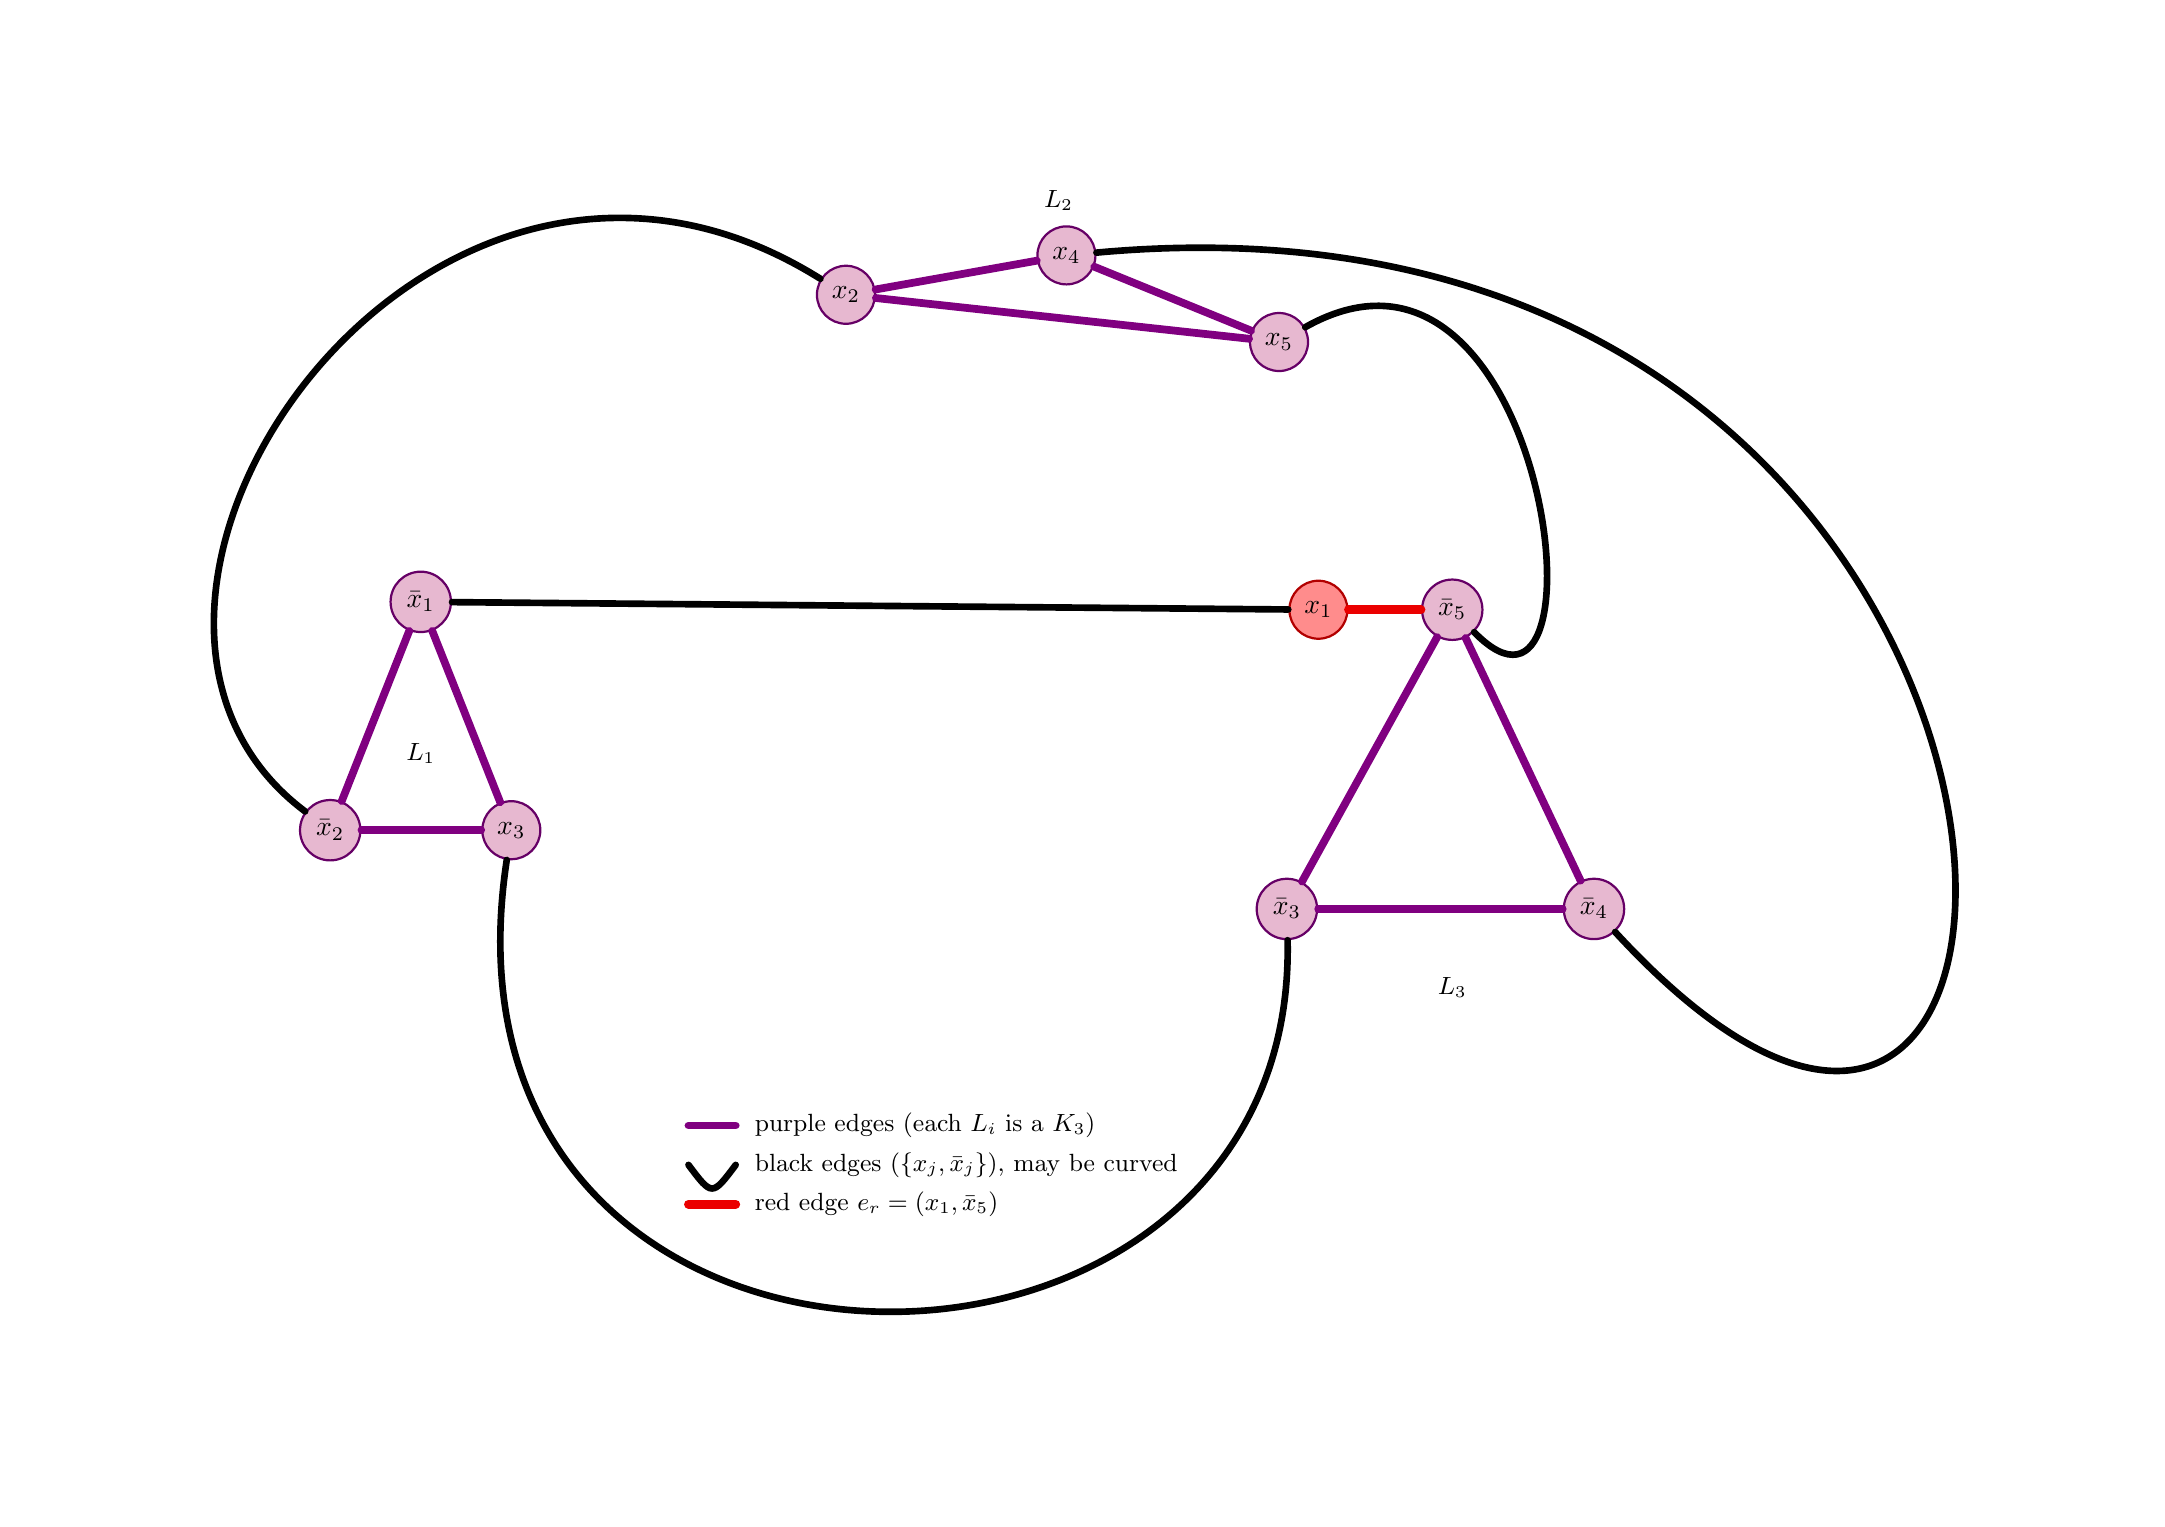
\begin{tikzpicture}[
  lbl/.style={font=\small, inner sep=1pt},
  redv/.style={circle, draw=red!70!black, line width=0.8pt, fill=red!45, minimum size=7mm},
  purpv/.style={circle, draw=violet!80!black, line width=0.8pt, fill=blue!12!purple!28, minimum size=7mm},
  purpleedge/.style={draw=violet, line width=2.8pt, line cap=round, line join=round},
  blackedge/.style={draw=black, line width=2.4pt, line cap=round},
  rededge/.style={draw=red!92!black, line width=3.2pt, line cap=round}
]

% Three clumps: $L_1$ (left), $L_2$ (top), $L_3$ (right) with $x_1$ beside $L_3$.
% Black (curved) drawn first; then nine straight purple edges and red on top.

% --- $L_1 = \{\bar{x}_1,\bar{x}_2,x_3\}$ ---
\node[purpv] (xb1) at (-5.55, 1.55) {$\bar{x}_1$};
\node[purpv] (xb2) at (-6.7, -1.35) {$\bar{x}_2$};
\node[purpv] (x3)  at (-4.4, -1.35) {$x_3$};

% --- $L_2 = \{x_2,x_4,x_5\}$ ---
\node[purpv] (x2) at (-0.15, 5.45) {$x_2$};
\node[purpv] (x4) at (2.65, 5.95) {$x_4$};
\node[purpv] (x5) at (5.35, 4.85) {$x_5$};

% --- $L_3 = \{\bar{x}_3,\bar{x}_4,\bar{x}_5\}$ and red vertex adjacent to $\bar{x}_5$ ---
\node[purpv] (xb3) at (5.45, -2.35) {$\bar{x}_3$};
\node[purpv] (xb4) at (9.35, -2.35) {$\bar{x}_4$};
\node[purpv] (xb5) at (7.55, 1.45) {$\bar{x}_5$};
\node[redv] (x1) at (5.85, 1.45) {$x_1$};

% --- black pair edges (disjoint corridors so arcs do not cross each other) ---
\draw[blackedge] (x1) -- (xb1);
\draw[blackedge] (x3) .. controls (-5.6,-9.2) and (5.6,-9.2) .. (xb3);
\draw[blackedge] (x2) .. controls (-5.5,8.8) and (-10.5,1.5) .. (xb2);
\draw[blackedge] (x4) .. controls (16.2,7.2) and (16.2,-9.8) .. (xb4);
\draw[blackedge] (x5) .. controls (8.8,6.8) and (9.6,-0.65) .. (xb5);

% --- purple: every edge of each $K_3$ (nine straight segments) ---
\draw[purpleedge] (xb1) -- (xb2);
\draw[purpleedge] (xb1) -- (x3);
\draw[purpleedge] (xb2) -- (x3);
\draw[purpleedge] (x2) -- (x4);
\draw[purpleedge] (x2) -- (x5);
\draw[purpleedge] (x4) -- (x5);
\draw[purpleedge] (xb3) -- (xb4);
\draw[purpleedge] (xb3) -- (xb5);
\draw[purpleedge] (xb4) -- (xb5);

\draw[rededge] (x1) -- (xb5);

% --- cluster labels ---
\node[lbl] at (-5.55, -0.38) {$L_1$};
\node[lbl] at (2.55, 6.65) {$L_2$};
\node[lbl] at (7.55, -3.35) {$L_3$};

% --- legend ---
\begin{scope}[shift={(-2.15,-5.1)}, anchor=west]
  \draw[purpleedge] (0,0) -- (6mm,0); \node[lbl, anchor=west] at (8mm,0) {purple edges (each $L_i$ is a $K_3$)};
  \draw[blackedge] (0,-5mm) .. controls +(3mm,-4mm) and +(-3mm,-4mm) .. (6mm,-5mm);
  \node[lbl, anchor=west] at (8mm,-5mm) {black edges ($\{x_j,\bar{x}_j\}$), may be curved};
  \draw[rededge] (0,-10mm) -- (6mm,-10mm);
  \node[lbl, anchor=west] at (8mm,-10mm) {red edge $e_r=(x_1,\bar{x}_5)$};
\end{scope}

\end{tikzpicture}%
}
\end{center}

\noindent Vertices follow Convention~\ref{c:ltt_structures}: $x_1$ is the unique red vertex; $\bar{x}_5$ is the purple endpoint of $e_r$; each triple $L_i$ spans a purple clique; each $\{x_j,\bar{x}_j\}$ is a black edge.

\begin{center}
\resizebox{0.62\linewidth}{!}{%
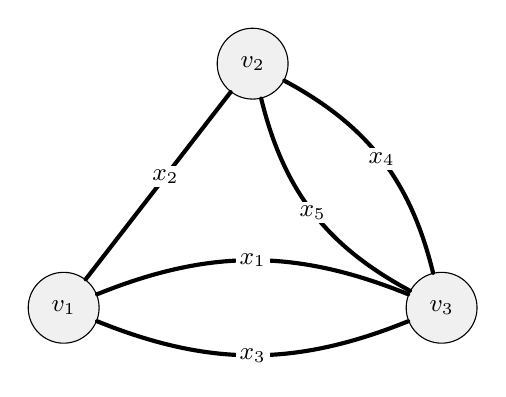
\begin{tikzpicture}[
  uvlbl/.style={font=\small, inner sep=1pt},
  uvedge/.style={line width=1.5pt, line cap=round},
  vtx/.style={circle, draw=black, fill=gray!12, minimum size=9mm, font=\small}
]
\node[vtx] (V1) at (-2.4, 0) {$v_1$};
\node[vtx] (V2) at (0, 3.1) {$v_2$};
\node[vtx] (V3) at (2.4, 0) {$v_3$};

% $x_2$: $L_2$ contains $x_2$, $L_1$ contains $\bar{x}_2$
\draw[uvedge] (V1) -- node[uvlbl, fill=white, inner sep=0.5mm, pos=0.55] {$x_2$} (V2);

% $x_1$, $x_3$: both between $v_1$ and $v_3$
\draw[uvedge] (V1) to[bend left=22]
  node[uvlbl, fill=white, midway, inner sep=0.5mm] {$x_1$} (V3);
\draw[uvedge] (V1) to[bend right=22]
  node[uvlbl, fill=white, midway, inner sep=0.5mm] {$x_3$} (V3);

% $x_4$, $x_5$: both between $v_2$ and $v_3$
\draw[uvedge] (V2) to[bend left=24]
  node[uvlbl, fill=white, midway, inner sep=0.5mm] {$x_4$} (V3);
\draw[uvedge] (V2) to[bend right=24]
  node[uvlbl, fill=white, midway, inner sep=0.5mm] {$x_5$} (V3);

\end{tikzpicture}%
}
\end{center}
\noindent Here $v_i$ corresponds to collapsing the purple clique on the labels in $L_i$, and collapsing the red edge identifies the red vertex $x_1$ with $\bar{x}_5\in L_3$, so the black edge $\{x_1,\bar{x}_1\}$ becomes a strand between $v_3$ and $v_1$ labeled $x_1$; the other black edges are read off from which $L_a$ contains $x_j$ and which contains $\bar{x}_j$.

\paragraph{Step 1.}
Start with a particular ltt structure $G$. Add a node to preAUT that is labeled by $G$.

For the first component of the automaton, we start with the seed ltt structure.
\begin{itemize}
  \item $\mathrm{GRAPHS}=\{G\}$;
  \item $\mathrm{graphs}_1=\{G\}$;
  \item $\mathrm{boxes}=\{\mathrm{graphs}_1\}$;
  \item layer 1 consists only of $G$, i.e. $\mathrm{GRAPHS}_1=\{G\}$.
\end{itemize}


\medskip
\noindent\textbf{Remark.}
$\mathrm{GRAPHS}$ will ultimately be the list of all nodes in the automaton.
\begin{itemize}
  \item each $\mathrm{graphs}_k$ will be a ``box'' of ep-isomorphic nodes;
  \item $\mathrm{boxes}$ will be the collection of these ep-isomorphism classes;
  \item before closing loops, where nodes represent the same ep-isomorphism class of
        ltt structures, the automaton looks like:
{\begin{itemize}
  \item each $\mathrm{GRAPHS}_2$ (layer 2) node is the terminal node of a directed edge from the $\mathrm{GRAPHS}_1$ (layer 1) node
  \item each $\mathrm{GRAPHS}_3$ (layer 3) node is the terminal node of a directed edge from at least one $\mathrm{GRAPHS}_2$ (layer 2) node
  \item in general, each $\mathrm{GRAPHS}_{k+1}$ (layer $k+1$) node is the terminal node of a directed edge from at least one $\mathrm{GRAPHS}_k$ (layer $k$) node\\
\end{itemize}}
\end{itemize}

\subsection{Recursive Step}

Recursively (with respect to $k$), complete in $\mathrm{PLTT}$ order Steps 2--3
for each $G\in \mathrm{GRAPHS}_k$.

\subsubsection{Step 2 (determining outgoing edges \& terminal graphs)}

We find the 4 outgoing edges (terminal ltt structures out of $G$) as follows:
\begin{itemize}
  \item Input the starting ltt structure $G$ (an admissible ltt structure):
        with the vertices labeled by $\mathcal{L}$ and following Convention \ref{c:ltt_structures}, but writing $d_r$ for the label of the red vertex (instead of $v_r$) and $d_p$ be for the label of the purple endpoint of the red edge (instead of $v_p$).
  \item There are exactly two vertices connected to the $d_p$-vertex by purple edges:
        \begin{enumerate}[label=\arabic*)]
          \item let $d_1$ be the label of the first;
          \item let $d_2$ be the label of the second;
        \end{enumerate}
        with order inherited from $\mathcal{L}$.
  \item For each of $d_1,d_2$, there are two potential directed edges out of $G$
        (hence one potential terminal ltt structure for each such edge). The triples 
        $$(\text{initial ltt structure}, \text{edge}, \text{terminal ltt structure})$$ 
        will be written as $(G, E_{jA}, G_{jA})$ for each $j\in\{1,2\}$ and $A\in\{a,b\}$, where the triples are determined as follows:
\end{itemize}

For $j\in\{1,2\}$:
\begin{itemize}
  \item[] $(G, E_{ja}, G_{ja})$:\\ 
  The outgoing edge $E_{ja}$ is labeled by $d_r \to d_j d_r$.\\
  The terminal ltt structure $G_{ja}$ has:
        \begin{itemize}
          \item red vertex $d_r$ and red edge $e_r=(d_r,\bar{d}_j)$;
          \item precisely these purple edges:
                \begin{itemize}
                  \item a purple edge $\{d,d'\}$ whenever $G$ has a purple edge
                        $\{d,d'\}$.
                \end{itemize}
        \end{itemize}
  \item[] $(G, E_{jb}, G_{jb})$:\\
  The outgoing edge $E_{jb}$ is labeled by $d_j \to d_r d_j$.\\
  The terminal ltt structure $G_{jb}$ has:
        \begin{itemize}
          \item red vertex $d_j$ and red edge $e_r=(d_j,\bar{d}_r)$;
          \item precisely these purple edges:
                \begin{itemize}
                  \item a purple edge $\{d_r,d\}$ whenever $G$ has a colored edge
                        $\{d_j,d\}$ and
                  \item a purple edge $\{d,d'\}$ whenever $G$ has a purple edge
                        $\{d,d'\}$ and neither $d=d_r$ nor $d'=d_r$.
                \end{itemize}
        \end{itemize}
\end{itemize}

Let
\[
\mathrm{terminal}(G):=\{G_{1;a},G_{1;b},G_{2;a},G_{2;b}\}
\]
(repetitions allowed).
\begin{itemize}
  \item Remove any graph from $\mathrm{terminal}(G)$ that is not in $\mathrm{PLTT}$.
  \item Each graph in $\mathrm{terminal}(G)$ is considered to be of level $k+1$.
  \item $\mathrm{terminal}(G)$ and level $k+1$ both inherit their order from
        $\mathrm{PLTT}$.
\end{itemize}

\begin{task}\label{t:Step2}
Run Step 2 for the seed ltt structure. Print the outcome.
\end{task}

Output in the appendix.

\subsubsection{Step 3 (Updating preAUT and the sets)}

In $\mathrm{PLTT}$ order, apply the following to each
$G'\in\mathrm{terminal}(G)$.

\begin{itemize}
  \item If $G'$ is ep-isomorphic to some $G''\in\mathrm{GRAPHS}$, but
        $G'\neq G''$:
        \begin{itemize}
          \item $\{G'\}$ is added to $\mathrm{GRAPHS}$, and
          \item $\{G'\}$ is added to $\mathrm{graphs}_j$ where
                $G''\in\mathrm{graphs}_j$, and
          \item add to preAUT a ``permutation edge'' $G'\to G''$ labeled by $\varphi$, where
                $\varphi$ is the permutation of $\mathcal{L}$ from the ep-isomorphism, and
        add to preAUT a directed edge $G\to G''$ with the edge label being that for $G\to G'$ given as in Step 2.
        \end{itemize}

  \item If there exists $G''\in\mathrm{GRAPHS}$ with $G'=G''$:
        add to preAUT a directed edge $G\to G''$ with the edge label being that for $G\to G'$ given as in Step 2.

  \item For the remaining $G'\in\mathrm{terminal}(G)$:
        \begin{itemize}
          \item $\{G'\}$ is added to $\mathrm{GRAPHS}$ and as a node to preAUT, and
          \item $\mathrm{graphs}_{i+1}=\{G'\}$ where $\mathrm{graphs}_i\in\mathrm{boxes}$
                and $\mathrm{graphs}_{i+1}\notin\mathrm{boxes}$, and
          \item $\{G'\}$ is added to $\mathrm{GRAPHS}_{k+1}$, and
          \item add to preAUT a directed edge $G\to G'$ with the edge label being that for $G\to G'$ given as in Step 2.
        \end{itemize}
\end{itemize}


\begin{task}\label{t:Step3}
Having completed running Step 2 for the seed ltt structure, run Step 3 on the output. Print the outcome in a manner that is easily readable by a human mathematician.
\end{task}

Output in the appendix.


\subsubsection{Step 4 (level shift \& program termination)}

After Steps 2--3 are completed for each $G\in\mathrm{GRAPHS}_k$, check whether
$\mathrm{GRAPHS}_{k+1}=\varnothing$.

If $\mathrm{GRAPHS}_{k+1}=\varnothing$, terminate.

If $\mathrm{GRAPHS}_{k+1}\neq\varnothing$, perform a level shift by replacing
$k$ with $k+1$ (equivalently, take the current level to be
$\mathrm{GRAPHS}_{k}:=\mathrm{GRAPHS}_{k+1}$), and then return to Steps 2--3
for each $G\in\mathrm{GRAPHS}_{k}$.

In other words, the recursive loop is: \\
For a fixed $k$:
\[
\ \text{run Steps 2--3 on all }G\in\mathrm{GRAPHS}_k
\ \longrightarrow\ \text{run Step 4}
\ \longrightarrow\ \text{if nonempty, set }k\leftarrow k+1\text{ and repeat.}
\]

\subsubsection{Step 5}


Output the preAUT according to this seed graph as nodes and edges (including ltt structure/map info), leaving out any components with no edges.

\subsubsection{Step 6}

If every ep-isomorphism class of admissible ltt structures is represented by a node in some component of preAUT constructed thus far, then take the disjoint union of these components as preAUT and move onto Step 7. Otherwise, run Step 1- Step 6 using a seed graph from an ep-isomorphism class that is not yet represented by any node.

\subsubsection{Step 7}

Output the disjoint union of the maximal strongly connected components of preAUT as AUT, again leaving out any components with no edges.

\appendix

\section{Figures for Task \ref{t:ltt_structure_list} (ep-isomorphism class representatives)}

The Python code \texttt{list\_admissible\_ltt\_classes.py} lists all $270$ connected distinguished admissible ltt structures; they fall into $14$ ep-isomorphism classes. Below, for each class, one representative is drawn in the same graphic style as the seed ltt structure earlier in this document (purple triangles for the three partition elements $L_1,L_2,L_3$, black edges for pairs $\{x_j,\bar{x}_j\}$, red edge $(x_1,x_2)$). The caption line records the distinguished indices returned by that program for graphs in the class.

\smallskip
\noindent\textit{Regenerating the TikZ blocks.} The file \texttt{ltt\_appendix\_generated.tex} is produced by running \texttt{python generate\_ltt\_appendix\_tex.py} from the repository root.

% Auto-generated by generate_ltt_appendix_tex.py — do not edit by hand (change generate_ltt_appendix_tex.py and re-run ``python generate_ltt_appendix_tex.py``).

\subsection*{Class 1 (II)}
\noindent Representative of this ep-isomorphism class.\\
\noindent Distinguished indices:\\ $\{1, 8, 11, 19, 53, 60, 63, 65, 71, 80, 103, 110, 124, 125, 154, 160, 164, 165, 241, 244, 251, 257, 261, 268\}$, $24$ total.
\begin{center}
\resizebox{\linewidth}{!}{%
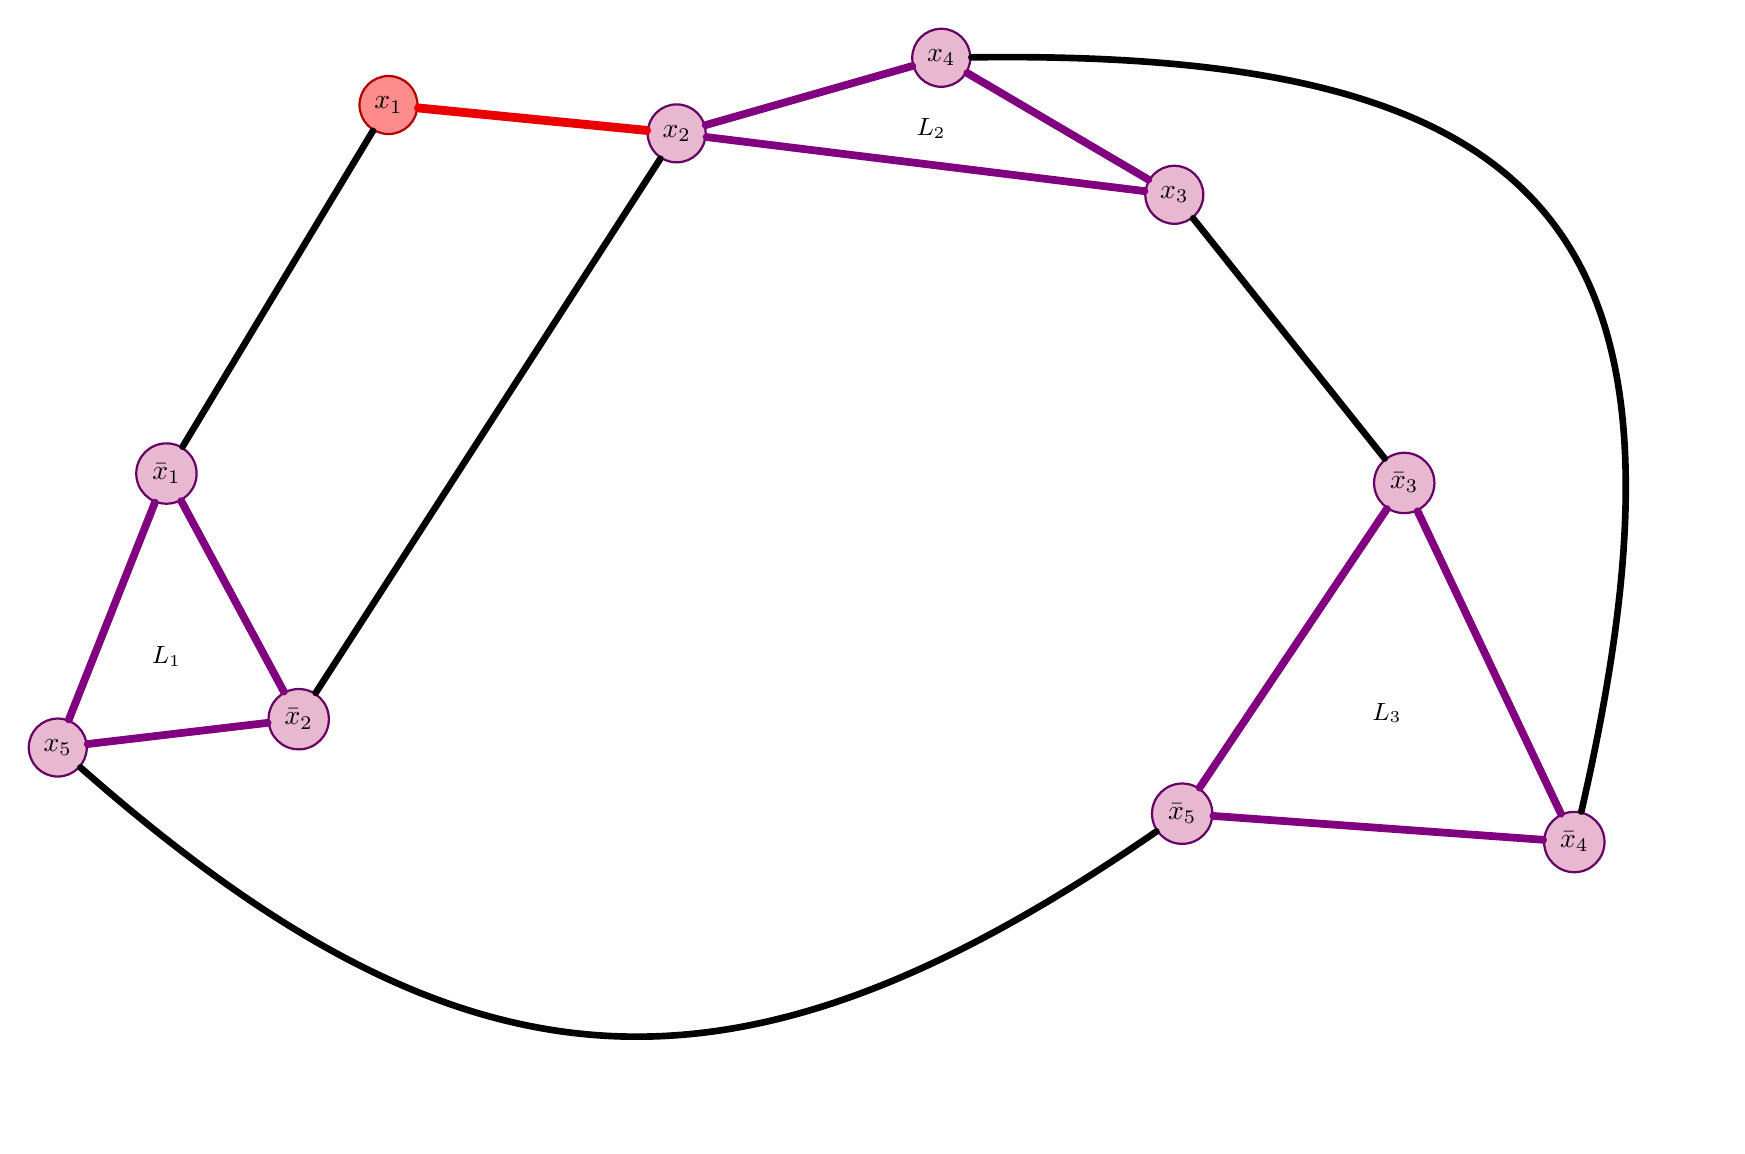
\begin{tikzpicture}[
  lbl/.style={font=\small, inner sep=1pt},
  redv/.style={circle, draw=red!70!black, line width=0.8pt, fill=red!45, minimum size=7mm},
  purpv/.style={circle, draw=violet!80!black, line width=0.8pt, fill=blue!12!purple!28, minimum size=7mm},
  purpleedge/.style={draw=violet, line width=2.8pt, line cap=round, line join=round},
  blackedge/.style={draw=black, line width=2.4pt, line cap=round},
  rededge/.style={draw=red!92!black, line width=3.2pt, line cap=round}
]

\node[redv] (nx1) at (-3.84, 6.54) {$x_{1}$};
\node[purpv] (nb1) at (-6.66, 1.86) {$\bar{x}_{1}$};
\node[purpv] (nx2) at (-0.18, 6.18) {$x_{2}$};
\node[purpv] (nb2) at (-4.98, -1.26) {$\bar{x}_{2}$};
\node[purpv] (nx3) at (6.14, 5.40) {$x_{3}$};
\node[purpv] (nb3) at (9.06, 1.74) {$\bar{x}_{3}$};
\node[purpv] (nx4) at (3.18, 7.14) {$x_{4}$};
\node[purpv] (nb4) at (11.22, -2.82) {$\bar{x}_{4}$};
\node[purpv] (nx5) at (-8.04, -1.62) {$x_{5}$};
\node[purpv] (nb5) at (6.24, -2.46) {$\bar{x}_{5}$};
\draw[purpleedge] (nb1) -- (nb2);
\draw[purpleedge] (nb1) -- (nx5);
\draw[purpleedge] (nb2) -- (nx5);
\draw[purpleedge] (nx2) -- (nx3);
\draw[purpleedge] (nx2) -- (nx4);
\draw[purpleedge] (nx3) -- (nx4);
\draw[purpleedge] (nb3) -- (nb4);
\draw[purpleedge] (nb3) -- (nb5);
\draw[purpleedge] (nb4) -- (nb5);
\draw[blackedge] (nx1) -- (nb1);
\draw[blackedge] (nx2) -- (nb2);
\draw[blackedge] (nx3) -- (nb3);
\draw[blackedge] (nx4) .. controls (11.06,7.25) and (12.99,4.86) .. (nb4);
\draw[blackedge] (nx5) .. controls (-2.86,-6.18) and (0.56,-6.38) .. (nb5);
\draw[rededge] (nx1) -- (nx2);
\node[lbl] at (-6.66, -0.46) {$L_1$};
\node[lbl] at (3.05, 6.24) {$L_2$};
\node[lbl] at (8.84, -1.18) {$L_3$};

\end{tikzpicture}%
}%

\end{center}
\medskip
\subsection*{Class 2 (I)}
\noindent Representative of this ep-isomorphism class.\\
\noindent Distinguished indices:\\ $\{2, 3, 5, 6, 12, 14, 15, 17, 51, 52, 57, 59, 61, 62, 66, 68, 73, 74, 76, 77, 101, 102, 107, 109\\ 121, 122, 127, 129, 151, 152, 156, 158, 161, 162, 167, 169, 245, 246, 249, 250, 252, 253, 259, 260, 262, 263, 265, 266\}$, $48$ total.
\begin{center}
\resizebox{\linewidth}{!}{%
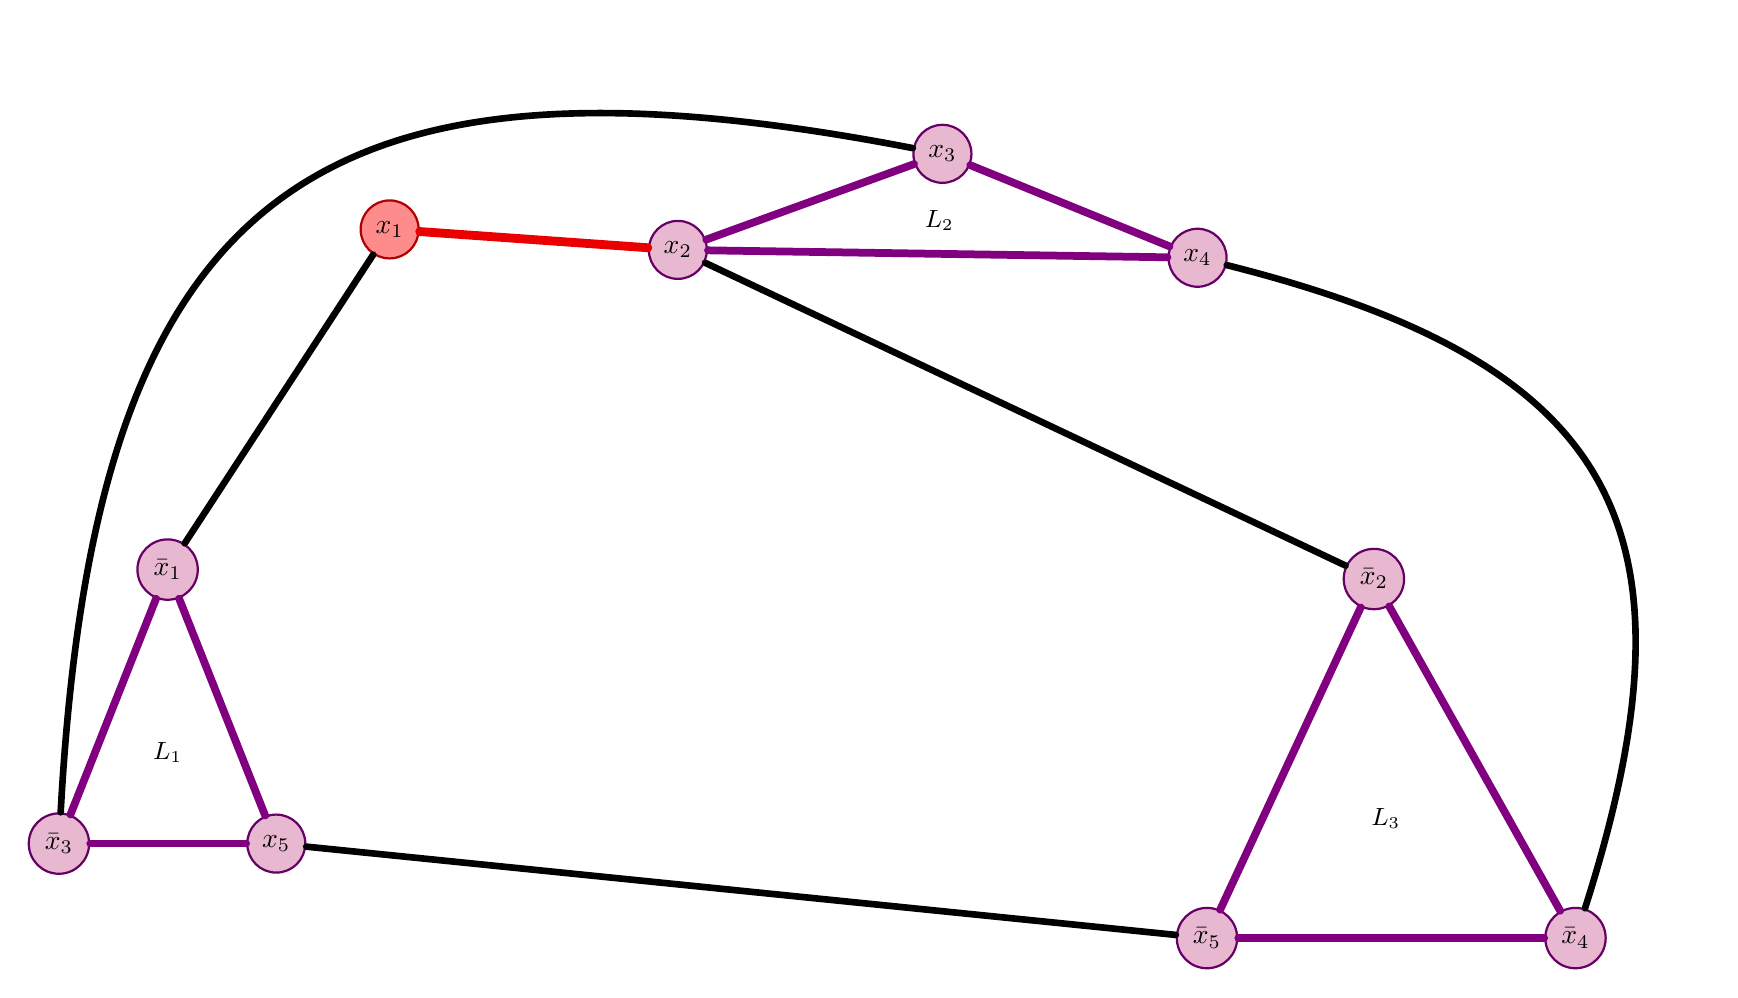
\begin{tikzpicture}[
  lbl/.style={font=\small, inner sep=1pt},
  redv/.style={circle, draw=red!70!black, line width=0.8pt, fill=red!45, minimum size=7mm},
  purpv/.style={circle, draw=violet!80!black, line width=0.8pt, fill=blue!12!purple!28, minimum size=7mm},
  purpleedge/.style={draw=violet, line width=2.8pt, line cap=round, line join=round},
  blackedge/.style={draw=black, line width=2.4pt, line cap=round},
  rededge/.style={draw=red!92!black, line width=3.2pt, line cap=round}
]

\node[redv] (nx1) at (-3.84, 6.18) {$x_{1}$};
\node[purpv] (nb1) at (-6.66, 1.86) {$\bar{x}_{1}$};
\node[purpv] (nx2) at (-0.18, 5.92) {$x_{2}$};
\node[purpv] (nb2) at (8.66, 1.74) {$\bar{x}_{2}$};
\node[purpv] (nx3) at (3.18, 7.14) {$x_{3}$};
\node[purpv] (nb3) at (-8.04, -1.62) {$\bar{x}_{3}$};
\node[purpv] (nx4) at (6.42, 5.82) {$x_{4}$};
\node[purpv] (nb4) at (11.22, -2.82) {$\bar{x}_{4}$};
\node[purpv] (nx5) at (-5.28, -1.62) {$x_{5}$};
\node[purpv] (nb5) at (6.54, -2.82) {$\bar{x}_{5}$};
\draw[purpleedge] (nb1) -- (nb3);
\draw[purpleedge] (nb1) -- (nx5);
\draw[purpleedge] (nb3) -- (nx5);
\draw[purpleedge] (nx2) -- (nx3);
\draw[purpleedge] (nx2) -- (nx4);
\draw[purpleedge] (nx3) -- (nx4);
\draw[purpleedge] (nb2) -- (nb4);
\draw[purpleedge] (nb2) -- (nb5);
\draw[purpleedge] (nb4) -- (nb5);
\draw[blackedge] (nx1) -- (nb1);
\draw[blackedge] (nx2) -- (nb2);
\draw[blackedge] (nx3) .. controls (-4.90,8.70) and (-7.59,6.60) .. (nb3);
\draw[blackedge] (nx4) .. controls (11.74,4.48) and (12.89,2.41) .. (nb4);
\draw[blackedge] (nx5) -- (nb5);
\draw[rededge] (nx1) -- (nx2);
\node[lbl] at (-6.66, -0.46) {$L_1$};
\node[lbl] at (3.14, 6.29) {$L_2$};
\node[lbl] at (8.81, -1.30) {$L_3$};

\end{tikzpicture}%
}%

\end{center}
\medskip
\subsection*{Class 3 (VII)}
\noindent Representative of this ep-isomorphism class.\\
\noindent Distinguished indices: $\{4, 13, 58, 67, 72, 108, 126, 159, 166, 243, 256, 269\}$, $12$ total.
\begin{center}
\resizebox{\linewidth}{!}{%
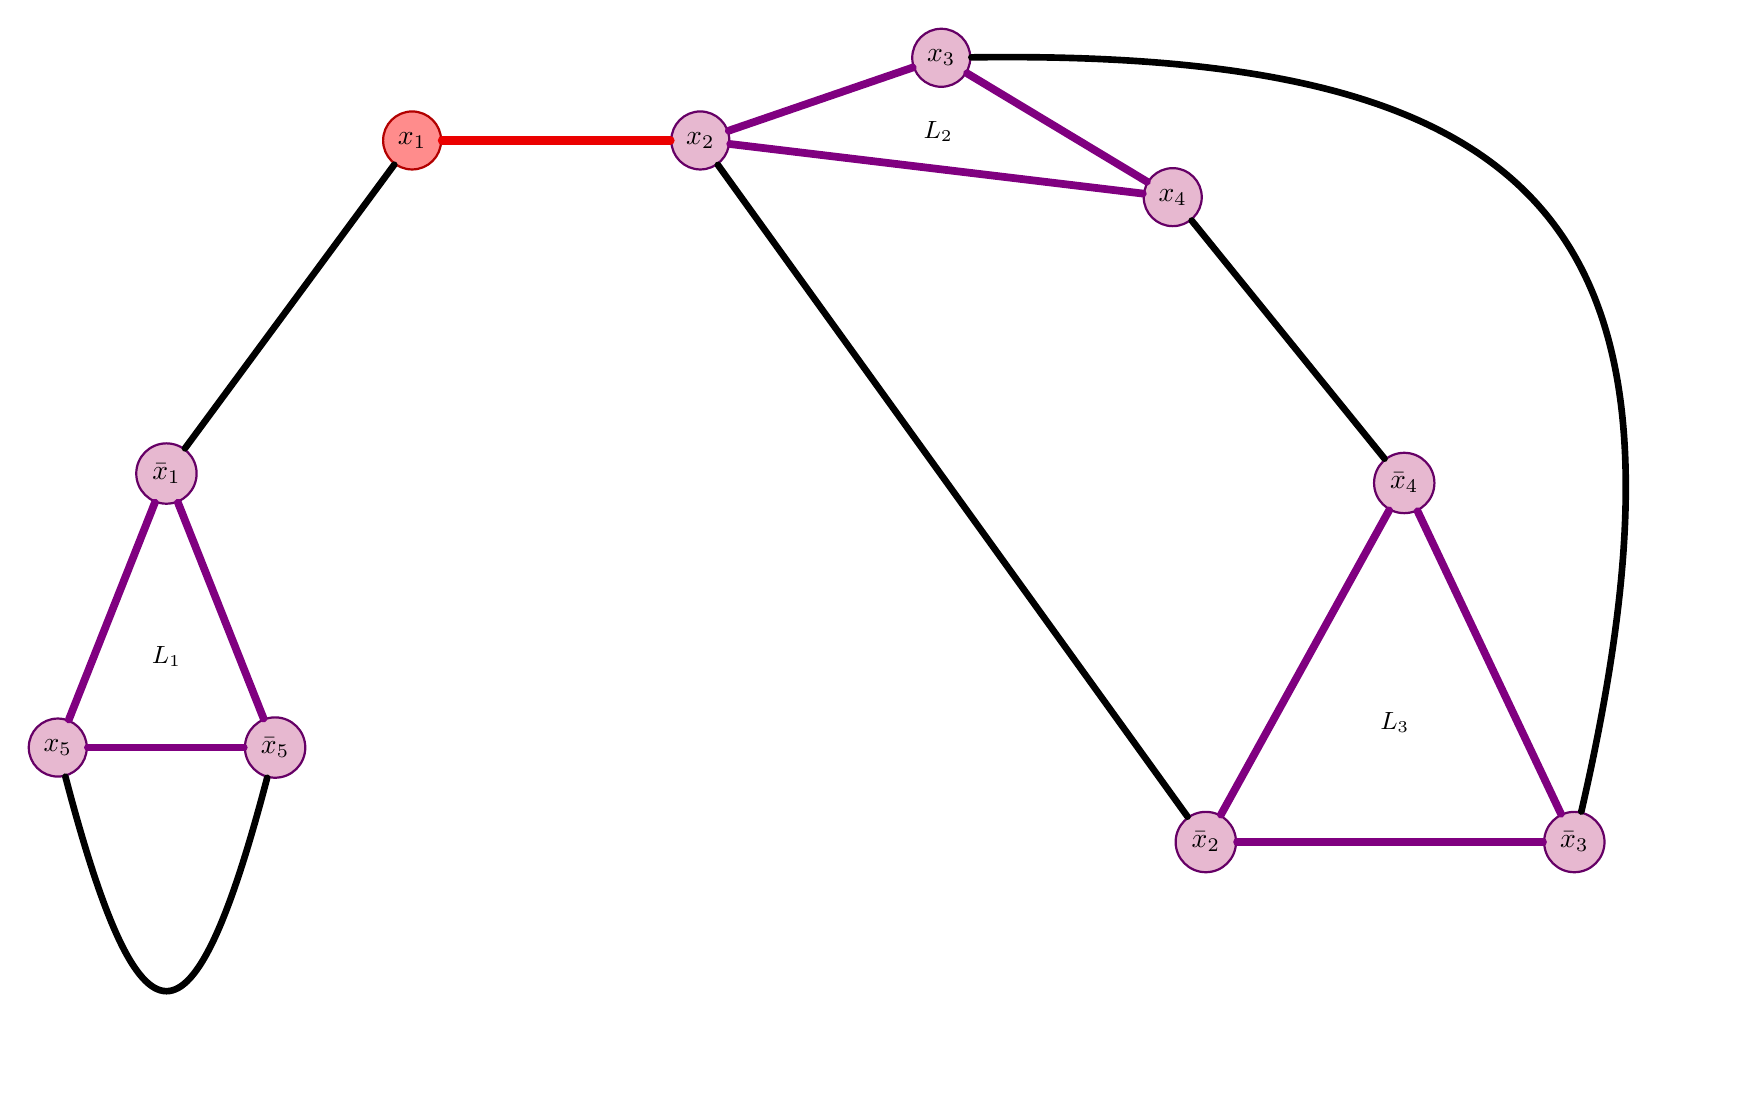
\begin{tikzpicture}[
  lbl/.style={font=\small, inner sep=1pt},
  redv/.style={circle, draw=red!70!black, line width=0.8pt, fill=red!45, minimum size=7mm},
  purpv/.style={circle, draw=violet!80!black, line width=0.8pt, fill=blue!12!purple!28, minimum size=7mm},
  purpleedge/.style={draw=violet, line width=2.8pt, line cap=round, line join=round},
  blackedge/.style={draw=black, line width=2.4pt, line cap=round},
  rededge/.style={draw=red!92!black, line width=3.2pt, line cap=round}
]

\node[redv] (nx1) at (-3.54, 6.09) {$x_{1}$};
\node[purpv] (nb1) at (-6.66, 1.86) {$\bar{x}_{1}$};
\node[purpv] (nx2) at (0.12, 6.09) {$x_{2}$};
\node[purpv] (nb2) at (6.54, -2.82) {$\bar{x}_{2}$};
\node[purpv] (nx3) at (3.18, 7.14) {$x_{3}$};
\node[purpv] (nb3) at (11.22, -2.82) {$\bar{x}_{3}$};
\node[purpv] (nx4) at (6.12, 5.37) {$x_{4}$};
\node[purpv] (nb4) at (9.06, 1.74) {$\bar{x}_{4}$};
\node[purpv] (nx5) at (-8.04, -1.62) {$x_{5}$};
\node[purpv] (nb5) at (-5.28, -1.62) {$\bar{x}_{5}$};
\draw[purpleedge] (nb1) -- (nx5);
\draw[purpleedge] (nb1) -- (nb5);
\draw[purpleedge] (nx5) -- (nb5);
\draw[purpleedge] (nx2) -- (nx3);
\draw[purpleedge] (nx2) -- (nx4);
\draw[purpleedge] (nx3) -- (nx4);
\draw[purpleedge] (nb2) -- (nb3);
\draw[purpleedge] (nb2) -- (nb4);
\draw[purpleedge] (nb3) -- (nb4);
\draw[blackedge] (nx1) -- (nb1);
\draw[blackedge] (nx2) -- (nb2);
\draw[blackedge] (nx3) .. controls (11.06,7.25) and (12.99,4.86) .. (nb3);
\draw[blackedge] (nx4) -- (nb4);
\draw[blackedge] (nx5) .. controls (-6.99,-5.62) and (-6.33,-5.62) .. (nb5);
\draw[rededge] (nx1) -- (nx2);
\node[lbl] at (-6.66, -0.46) {$L_1$};
\node[lbl] at (3.14, 6.20) {$L_2$};
\node[lbl] at (8.94, -1.30) {$L_3$};

\end{tikzpicture}%
}%

\end{center}
\medskip
\subsection*{Class 4 (VIII)}
\noindent Representative of this ep-isomorphism class.\\
\noindent Distinguished indices: $\{7, 16, 56, 69, 75, 106, 128, 157, 168, 242, 255, 270\}$, $12$ total.
\begin{center}
\resizebox{\linewidth}{!}{%
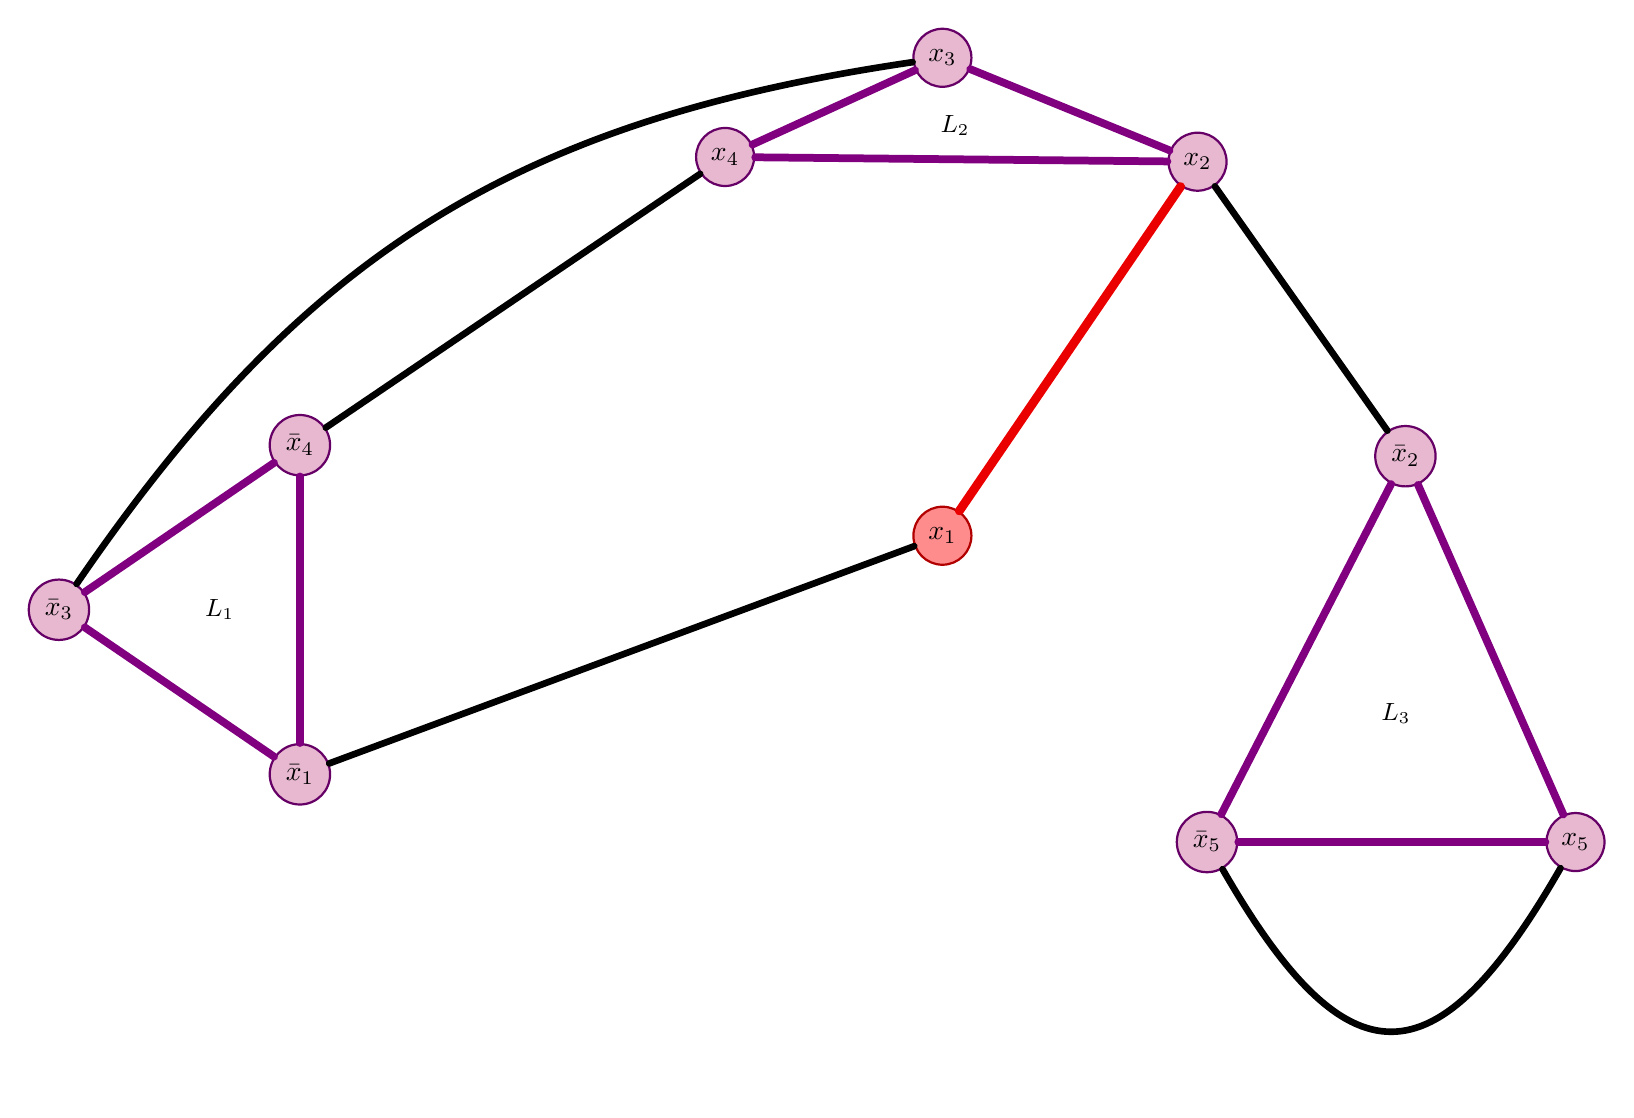
\begin{tikzpicture}[
  lbl/.style={font=\small, inner sep=1pt},
  redv/.style={circle, draw=red!70!black, line width=0.8pt, fill=red!45, minimum size=7mm},
  purpv/.style={circle, draw=violet!80!black, line width=0.8pt, fill=blue!12!purple!28, minimum size=7mm},
  purpleedge/.style={draw=violet, line width=2.8pt, line cap=round, line join=round},
  blackedge/.style={draw=black, line width=2.4pt, line cap=round},
  rededge/.style={draw=red!92!black, line width=3.2pt, line cap=round}
]

\node[redv] (nx1) at (3.18, 1.07) {$x_{1}$};
\node[purpv] (nb1) at (-4.98, -1.96) {$\bar{x}_{1}$};
\node[purpv] (nx2) at (6.42, 5.82) {$x_{2}$};
\node[purpv] (nb2) at (9.06, 2.08) {$\bar{x}_{2}$};
\node[purpv] (nx3) at (3.18, 7.14) {$x_{3}$};
\node[purpv] (nb3) at (-8.04, 0.13) {$\bar{x}_{3}$};
\node[purpv] (nx4) at (0.42, 5.88) {$x_{4}$};
\node[purpv] (nb4) at (-4.98, 2.22) {$\bar{x}_{4}$};
\node[purpv] (nx5) at (11.22, -2.82) {$x_{5}$};
\node[purpv] (nb5) at (6.54, -2.82) {$\bar{x}_{5}$};
\draw[purpleedge] (nb1) -- (nb3);
\draw[purpleedge] (nb1) -- (nb4);
\draw[purpleedge] (nb3) -- (nb4);
\draw[purpleedge] (nx2) -- (nx3);
\draw[purpleedge] (nx2) -- (nx4);
\draw[purpleedge] (nx3) -- (nx4);
\draw[purpleedge] (nb2) -- (nx5);
\draw[purpleedge] (nb2) -- (nb5);
\draw[purpleedge] (nx5) -- (nb5);
\draw[blackedge] (nx1) -- (nb1);
\draw[blackedge] (nx2) -- (nb2);
\draw[blackedge] (nx3) .. controls (-2.25,6.34) and (-4.94,4.66) .. (nb3);
\draw[blackedge] (nx4) -- (nb4);
\draw[blackedge] (nx5) .. controls (9.44,-5.92) and (8.32,-5.92) .. (nb5);
\draw[rededge] (nx1) -- (nx2);
\node[lbl] at (-6.00, 0.13) {$L_1$};
\node[lbl] at (3.34, 6.28) {$L_2$};
\node[lbl] at (8.94, -1.19) {$L_3$};

\end{tikzpicture}%
}%

\end{center}
\medskip
\subsection*{Class 5 (VI)}
\noindent Representative of this ep-isomorphism class.\\
\noindent Distinguished indices:\\ $\{9, 10, 18, 20, 54, 55, 64, 70, 78, 79, 104, 105, 123, 130, 153, 155, 163, 170, 247, 248, 254, 258, 264, 267\}$, $24$ total.
\begin{center}
\resizebox{\linewidth}{!}{%
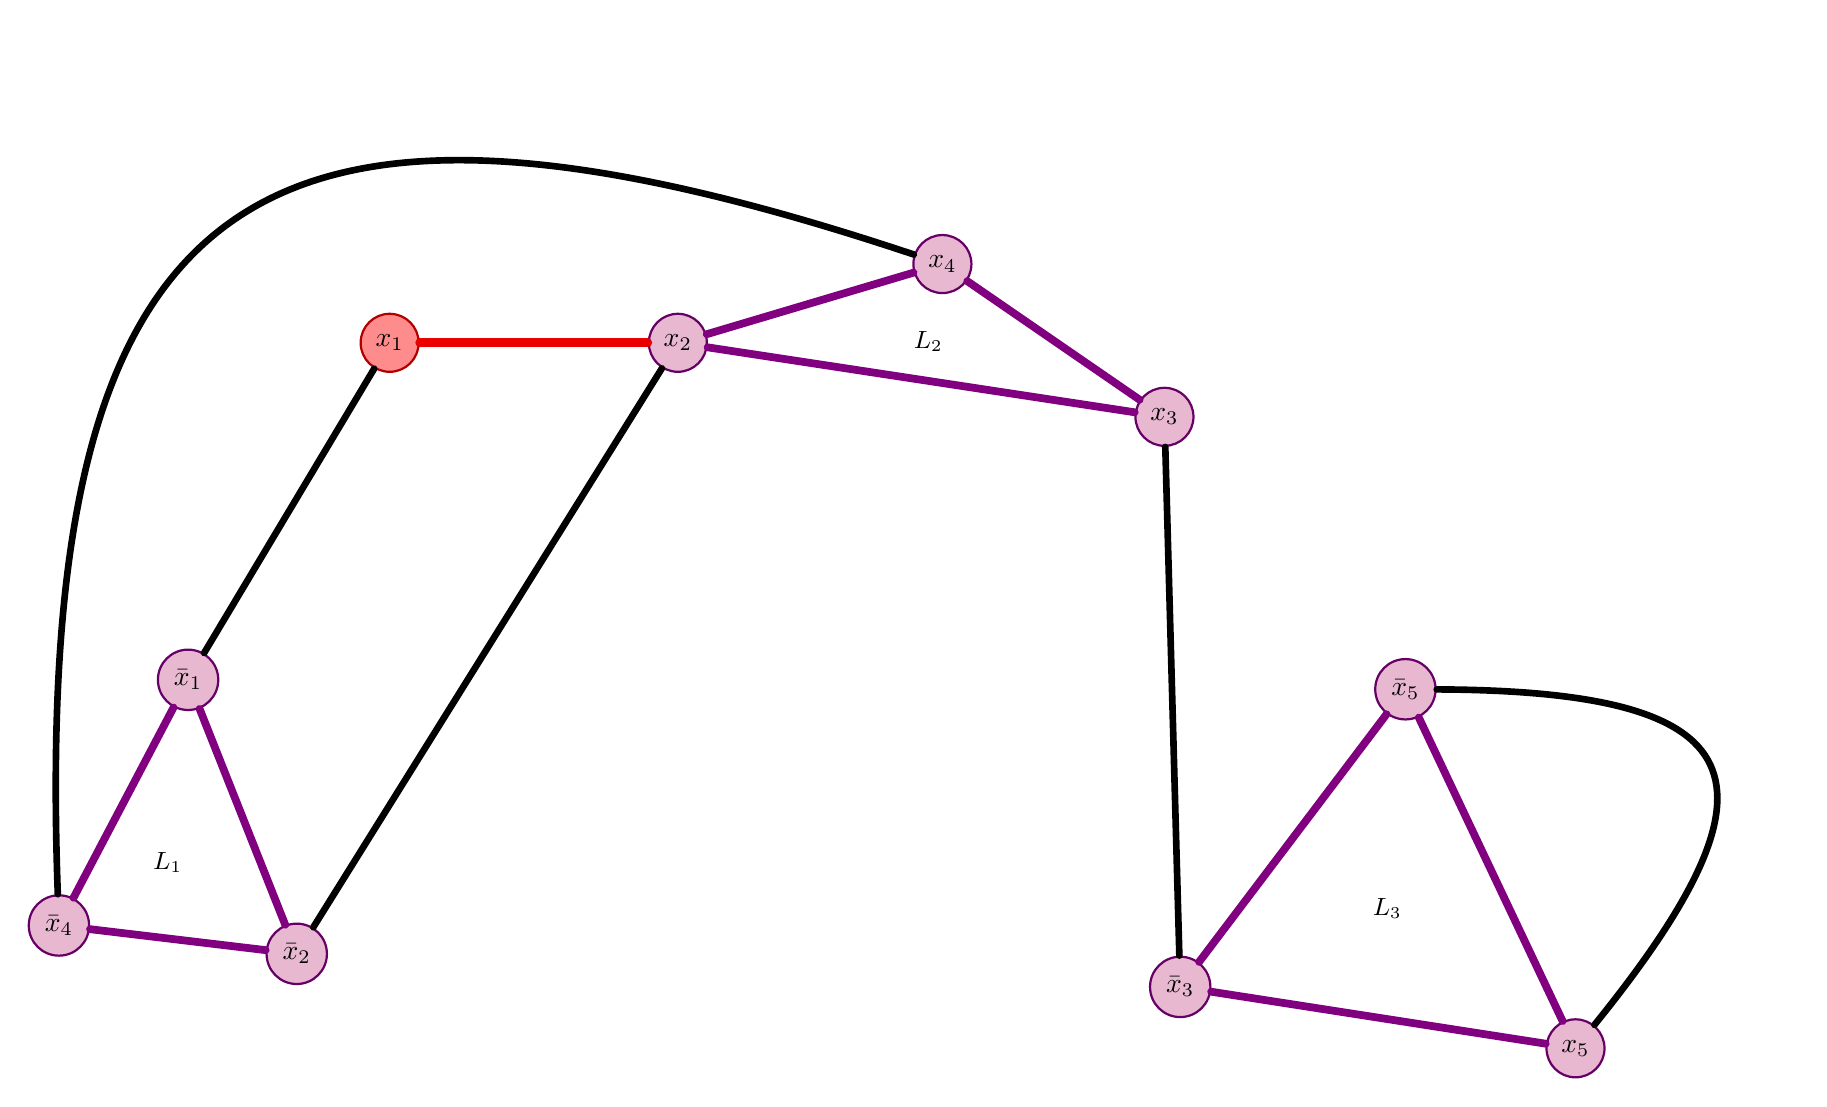
\begin{tikzpicture}[
  lbl/.style={font=\small, inner sep=1pt},
  redv/.style={circle, draw=red!70!black, line width=0.8pt, fill=red!45, minimum size=7mm},
  purpv/.style={circle, draw=violet!80!black, line width=0.8pt, fill=blue!12!purple!28, minimum size=7mm},
  purpleedge/.style={draw=violet, line width=2.8pt, line cap=round, line join=round},
  blackedge/.style={draw=black, line width=2.4pt, line cap=round},
  rededge/.style={draw=red!92!black, line width=3.2pt, line cap=round}
]

\node[redv] (nx1) at (-3.84, 6.14) {$x_{1}$};
\node[purpv] (nb1) at (-6.40, 1.86) {$\bar{x}_{1}$};
\node[purpv] (nx2) at (-0.18, 6.14) {$x_{2}$};
\node[purpv] (nb2) at (-5.02, -1.62) {$\bar{x}_{2}$};
\node[purpv] (nx3) at (6.00, 5.20) {$x_{3}$};
\node[purpv] (nb3) at (6.20, -2.04) {$\bar{x}_{3}$};
\node[purpv] (nx4) at (3.18, 7.14) {$x_{4}$};
\node[purpv] (nb4) at (-8.04, -1.26) {$\bar{x}_{4}$};
\node[purpv] (nx5) at (11.22, -2.82) {$x_{5}$};
\node[purpv] (nb5) at (9.06, 1.74) {$\bar{x}_{5}$};
\draw[purpleedge] (nb1) -- (nb2);
\draw[purpleedge] (nb1) -- (nb4);
\draw[purpleedge] (nb2) -- (nb4);
\draw[purpleedge] (nx2) -- (nx3);
\draw[purpleedge] (nx2) -- (nx4);
\draw[purpleedge] (nx3) -- (nx4);
\draw[purpleedge] (nb3) -- (nx5);
\draw[purpleedge] (nb3) -- (nb5);
\draw[purpleedge] (nx5) -- (nb5);
\draw[blackedge] (nx1) -- (nb1);
\draw[blackedge] (nx2) -- (nb2);
\draw[blackedge] (nx3) -- (nb3);
\draw[blackedge] (nx4) .. controls (-5.69,10.10) and (-8.38,8.09) .. (nb4);
\draw[blackedge] (nx5) .. controls (14.01,0.63) and (13.50,1.72) .. (nb5);
\draw[rededge] (nx1) -- (nx2);
\node[lbl] at (-6.66, -0.46) {$L_1$};
\node[lbl] at (3.00, 6.16) {$L_2$};
\node[lbl] at (8.83, -1.04) {$L_3$};

\end{tikzpicture}%
}%

\end{center}
\medskip
\subsection*{Class 6 (III)}
\noindent Representative of this ep-isomorphism class.\\
\noindent Distinguished indices:\\ $\{21, 22, 27, 29, 81, 83, 87, 90, 131, 134, 136, 140, 181, 184, 186, 190, 191, 194, 195, 199, 201, 202, 207, 209\}$, $24$ total.
\begin{center}
\resizebox{\linewidth}{!}{%
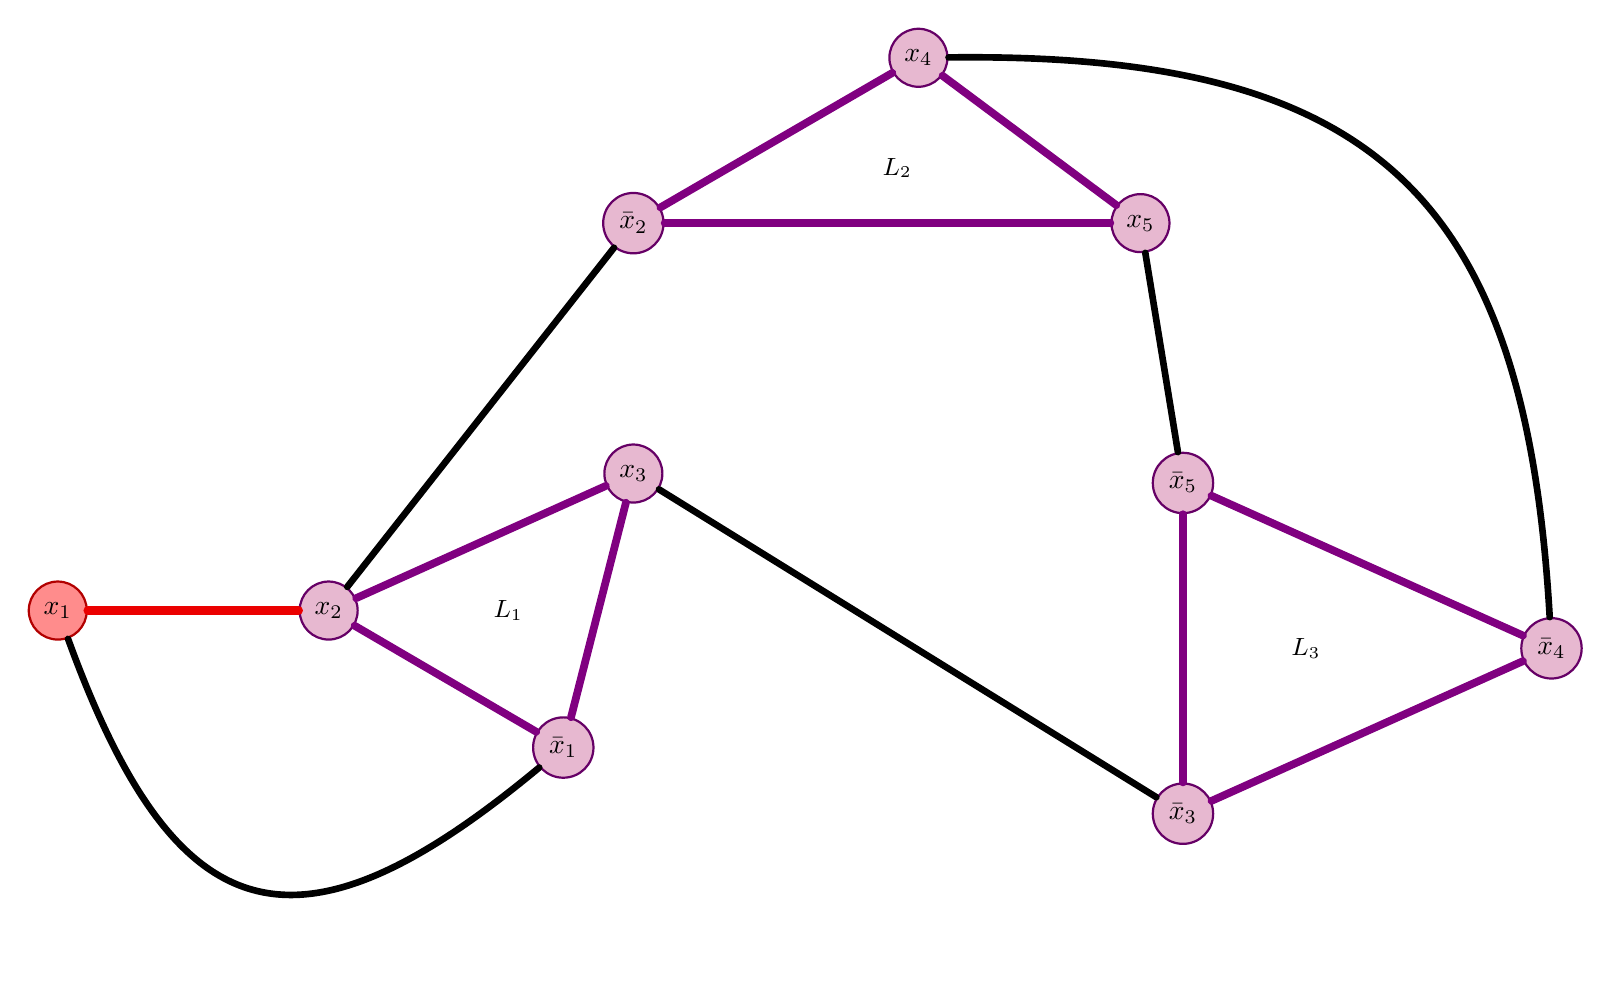
\begin{tikzpicture}[
  lbl/.style={font=\small, inner sep=1pt},
  redv/.style={circle, draw=red!70!black, line width=0.8pt, fill=red!45, minimum size=7mm},
  purpv/.style={circle, draw=violet!80!black, line width=0.8pt, fill=blue!12!purple!28, minimum size=7mm},
  purpleedge/.style={draw=violet, line width=2.8pt, line cap=round, line join=round},
  blackedge/.style={draw=black, line width=2.4pt, line cap=round},
  rededge/.style={draw=red!92!black, line width=3.2pt, line cap=round}
]

\node[redv] (nx1) at (-7.75, 0.12) {$x_{1}$};
\node[purpv] (nb1) at (-1.33, -1.62) {$\bar{x}_{1}$};
\node[purpv] (nx2) at (-4.31, 0.12) {$x_{2}$};
\node[purpv] (nb2) at (-0.44, 5.04) {$\bar{x}_{2}$};
\node[purpv] (nx3) at (-0.44, 1.86) {$x_{3}$};
\node[purpv] (nb3) at (6.54, -2.46) {$\bar{x}_{3}$};
\node[purpv] (nx4) at (3.18, 7.14) {$x_{4}$};
\node[purpv] (nb4) at (11.22, -0.36) {$\bar{x}_{4}$};
\node[purpv] (nx5) at (6.00, 5.04) {$x_{5}$};
\node[purpv] (nb5) at (6.54, 1.74) {$\bar{x}_{5}$};
\draw[purpleedge] (nb1) -- (nx2);
\draw[purpleedge] (nb1) -- (nx3);
\draw[purpleedge] (nx2) -- (nx3);
\draw[purpleedge] (nb2) -- (nx4);
\draw[purpleedge] (nb2) -- (nx5);
\draw[purpleedge] (nx4) -- (nx5);
\draw[purpleedge] (nb3) -- (nb4);
\draw[purpleedge] (nb3) -- (nb5);
\draw[purpleedge] (nb4) -- (nb5);
\draw[blackedge] (nx1) .. controls (-6.25,-4.01) and (-4.71,-4.43) .. (nb1);
\draw[blackedge] (nx2) -- (nb2);
\draw[blackedge] (nx3) -- (nb3);
\draw[blackedge] (nx4) .. controls (8.96,7.21) and (10.89,5.41) .. (nb4);
\draw[blackedge] (nx5) -- (nb5);
\draw[rededge] (nx1) -- (nx2);
\node[lbl] at (-2.03, 0.12) {$L_1$};
\node[lbl] at (2.91, 5.74) {$L_2$};
\node[lbl] at (8.10, -0.36) {$L_3$};

\end{tikzpicture}%
}%

\end{center}
\medskip
\subsection*{Class 7 (X)}
\noindent Representative of this ep-isomorphism class.\\
\noindent Distinguished indices:\\ $\{23, 24, 25, 30, 82, 84, 86, 89, 132, 133, 137, 138, 182, 185, 188, 189, 192, 196, 197, 200, 203, 204, 205, 210\}$, $24$ total.
\begin{center}
\resizebox{\linewidth}{!}{%
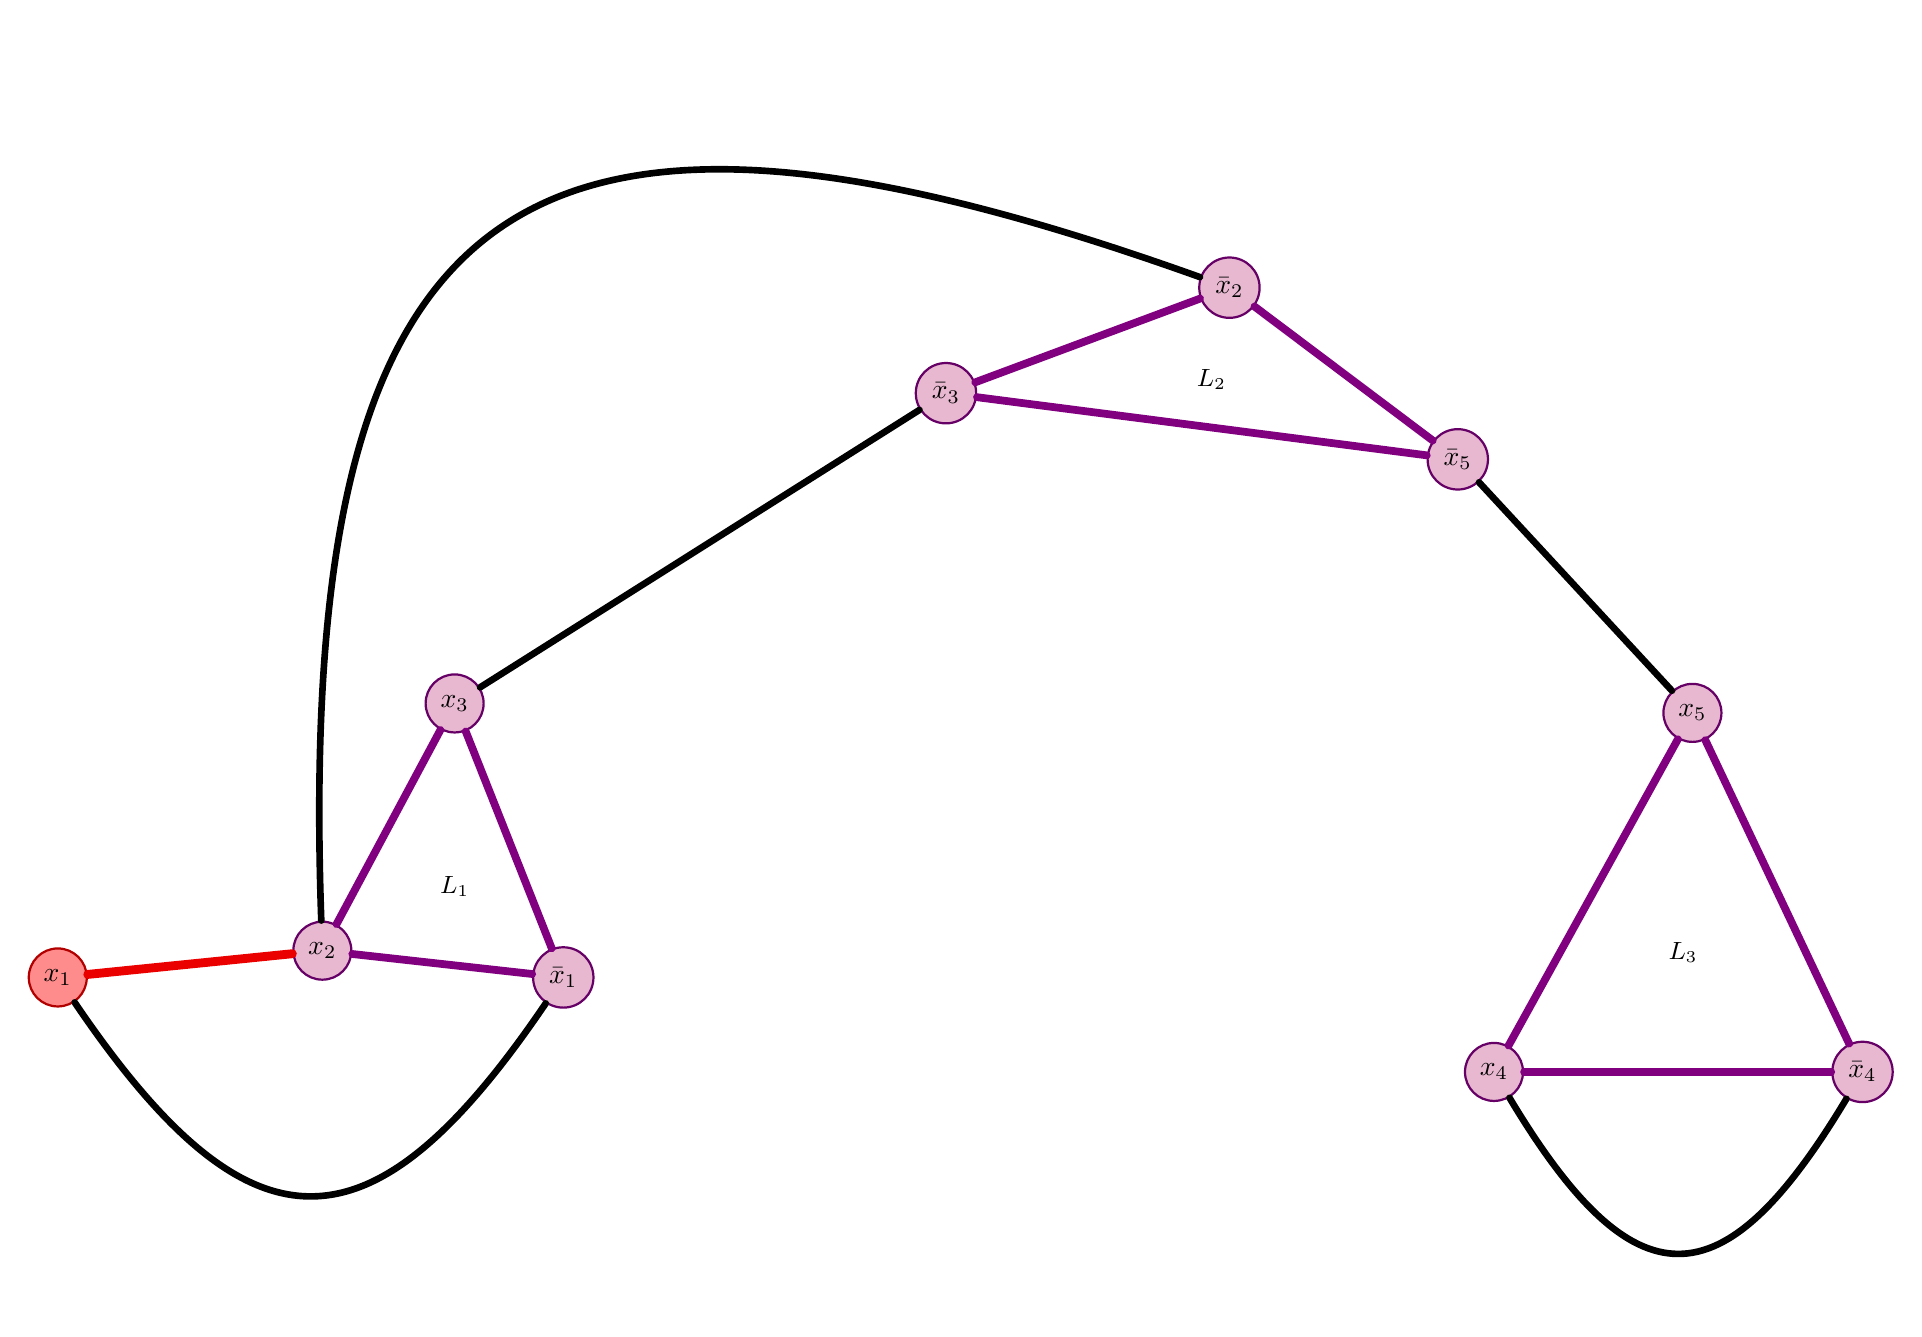
\begin{tikzpicture}[
  lbl/.style={font=\small, inner sep=1pt},
  redv/.style={circle, draw=red!70!black, line width=0.8pt, fill=red!45, minimum size=7mm},
  purpv/.style={circle, draw=violet!80!black, line width=0.8pt, fill=blue!12!purple!28, minimum size=7mm},
  purpleedge/.style={draw=violet, line width=2.8pt, line cap=round, line join=round},
  blackedge/.style={draw=black, line width=2.4pt, line cap=round},
  rededge/.style={draw=red!92!black, line width=3.2pt, line cap=round}
]

\node[redv] (nx1) at (-11.70, -1.62) {$x_{1}$};
\node[purpv] (nb1) at (-5.28, -1.62) {$\bar{x}_{1}$};
\node[purpv] (nx2) at (-8.34, -1.28) {$x_{2}$};
\node[purpv] (nb2) at (3.18, 7.14) {$\bar{x}_{2}$};
\node[purpv] (nx3) at (-6.66, 1.86) {$x_{3}$};
\node[purpv] (nb3) at (-0.42, 5.80) {$\bar{x}_{3}$};
\node[purpv] (nx4) at (6.54, -2.82) {$x_{4}$};
\node[purpv] (nb4) at (11.22, -2.82) {$\bar{x}_{4}$};
\node[purpv] (nx5) at (9.06, 1.74) {$x_{5}$};
\node[purpv] (nb5) at (6.08, 4.96) {$\bar{x}_{5}$};
\draw[purpleedge] (nb1) -- (nx2);
\draw[purpleedge] (nb1) -- (nx3);
\draw[purpleedge] (nx2) -- (nx3);
\draw[purpleedge] (nb2) -- (nb3);
\draw[purpleedge] (nb2) -- (nb5);
\draw[purpleedge] (nb3) -- (nb5);
\draw[purpleedge] (nx4) -- (nb4);
\draw[purpleedge] (nx4) -- (nx5);
\draw[purpleedge] (nb4) -- (nx5);
\draw[blackedge] (nx1) .. controls (-9.26,-5.22) and (-7.72,-5.22) .. (nb1);
\draw[blackedge] (nx2) .. controls (-8.68,8.38) and (-5.92,10.40) .. (nb2);
\draw[blackedge] (nx3) -- (nb3);
\draw[blackedge] (nx4) .. controls (8.32,-5.79) and (9.44,-5.79) .. (nb4);
\draw[blackedge] (nx5) -- (nb5);
\draw[rededge] (nx1) -- (nx2);
\node[lbl] at (-6.66, -0.46) {$L_1$};
\node[lbl] at (2.95, 5.97) {$L_2$};
\node[lbl] at (8.94, -1.30) {$L_3$};

\end{tikzpicture}%
}%

\end{center}
\medskip
\subsection*{Class 8 (XII)}
\noindent Representative of this ep-isomorphism class.\\
\noindent Distinguished indices: $\{26, 28, 85, 88, 135, 139, 183, 187, 193, 198, 206, 208\}$, $12$ total.
\begin{center}
\resizebox{\linewidth}{!}{%
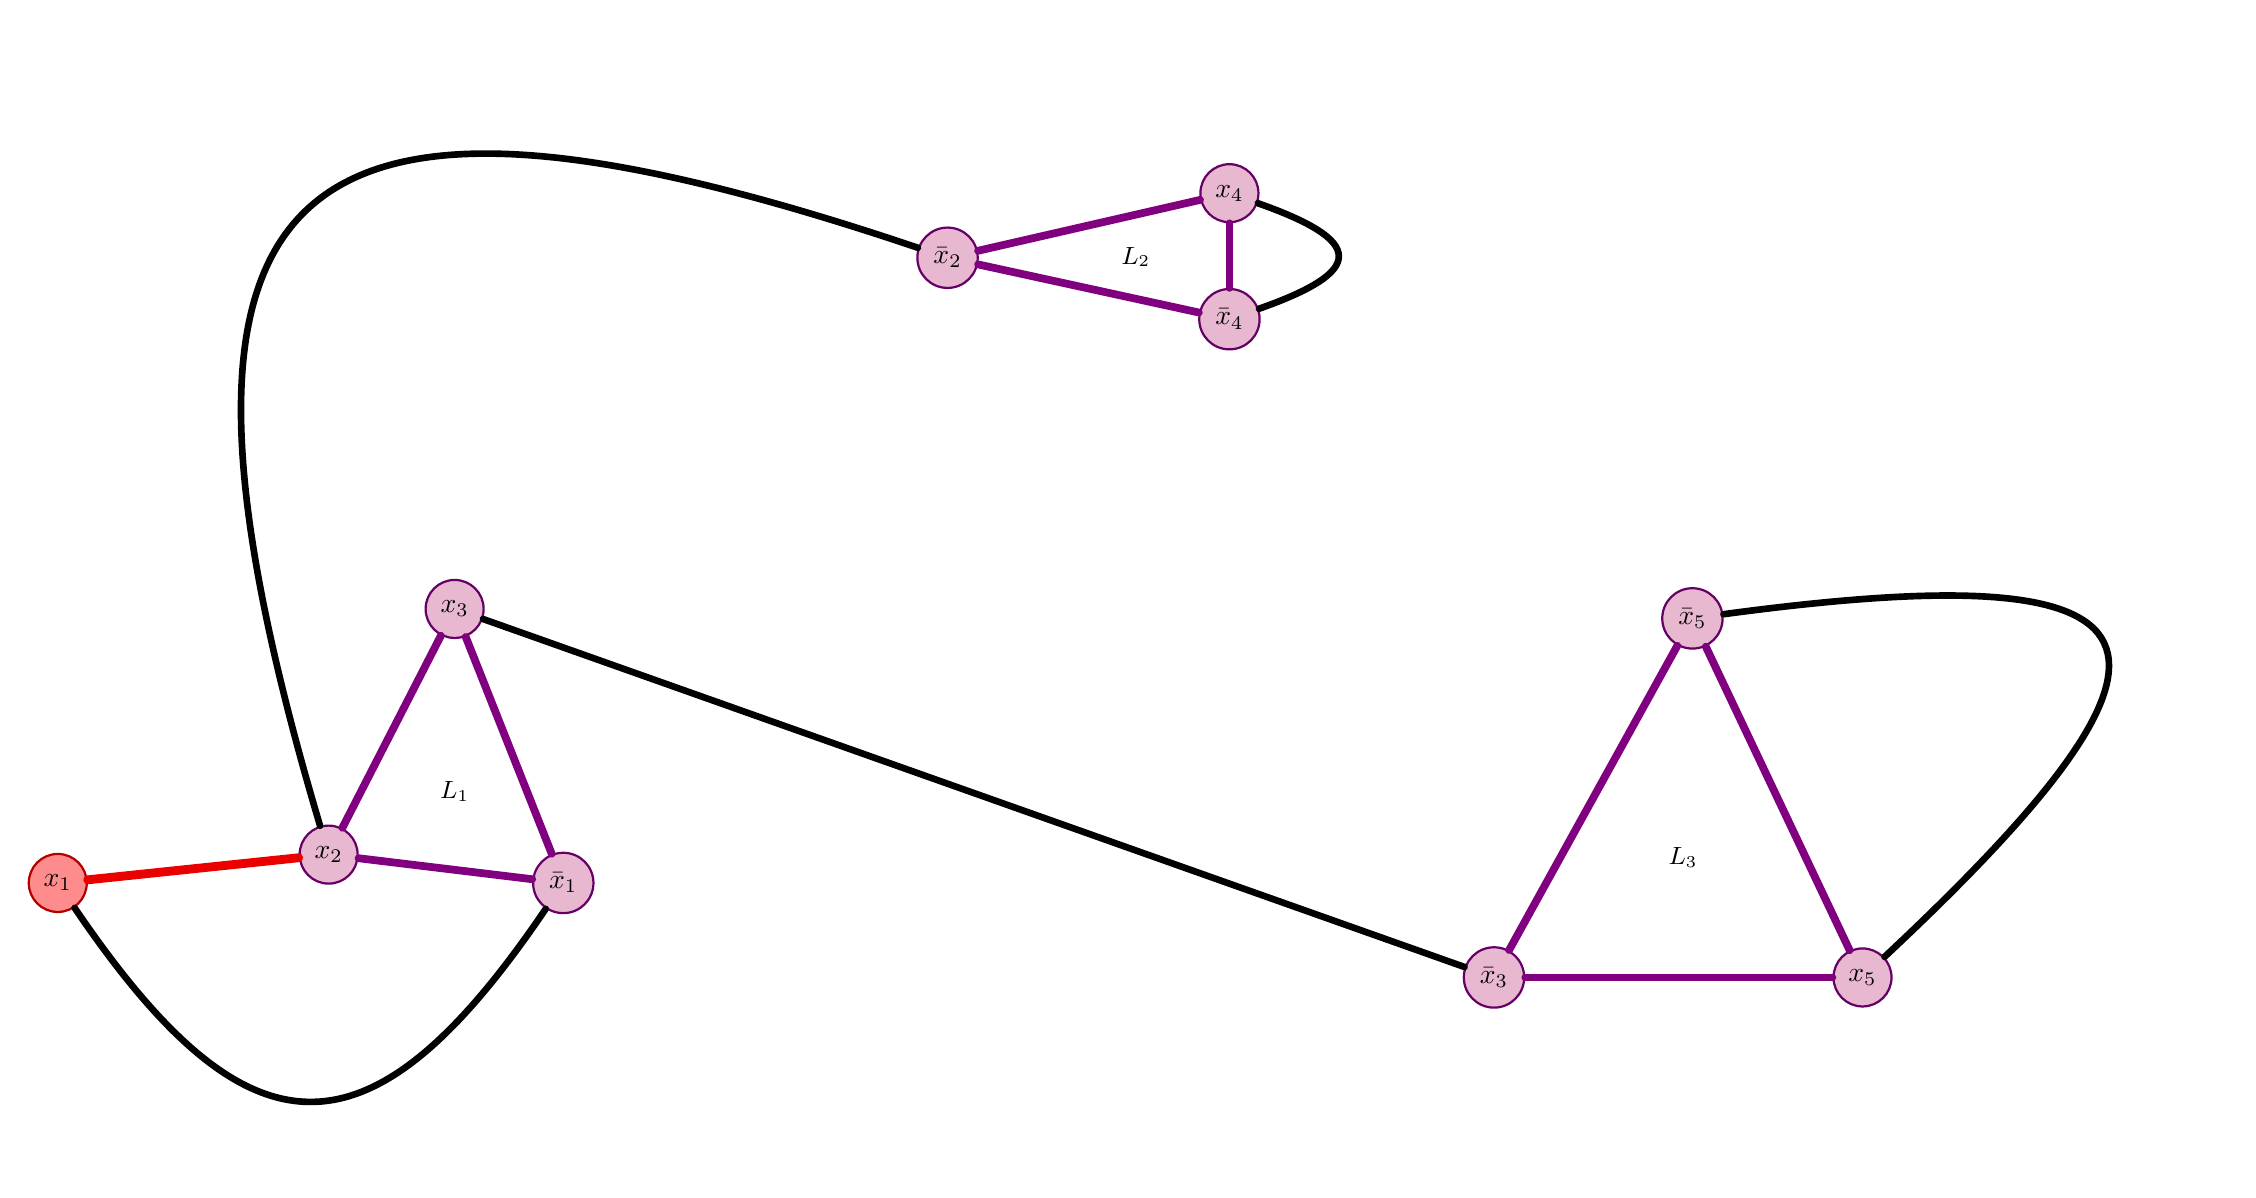
\begin{tikzpicture}[
  lbl/.style={font=\small, inner sep=1pt},
  redv/.style={circle, draw=red!70!black, line width=0.8pt, fill=red!45, minimum size=7mm},
  purpv/.style={circle, draw=violet!80!black, line width=0.8pt, fill=blue!12!purple!28, minimum size=7mm},
  purpleedge/.style={draw=violet, line width=2.8pt, line cap=round, line join=round},
  blackedge/.style={draw=black, line width=2.4pt, line cap=round},
  rededge/.style={draw=red!92!black, line width=3.2pt, line cap=round}
]

\node[redv] (nx1) at (-11.70, -1.62) {$x_{1}$};
\node[purpv] (nb1) at (-5.28, -1.62) {$\bar{x}_{1}$};
\node[purpv] (nx2) at (-8.26, -1.26) {$x_{2}$};
\node[purpv] (nb2) at (-0.40, 6.32) {$\bar{x}_{2}$};
\node[purpv] (nx3) at (-6.66, 1.86) {$x_{3}$};
\node[purpv] (nb3) at (6.54, -2.82) {$\bar{x}_{3}$};
\node[purpv] (nx4) at (3.18, 7.14) {$x_{4}$};
\node[purpv] (nb4) at (3.18, 5.54) {$\bar{x}_{4}$};
\node[purpv] (nx5) at (11.22, -2.82) {$x_{5}$};
\node[purpv] (nb5) at (9.06, 1.74) {$\bar{x}_{5}$};
\draw[purpleedge] (nb1) -- (nx2);
\draw[purpleedge] (nb1) -- (nx3);
\draw[purpleedge] (nx2) -- (nx3);
\draw[purpleedge] (nb2) -- (nx4);
\draw[purpleedge] (nb2) -- (nb4);
\draw[purpleedge] (nx4) -- (nb4);
\draw[purpleedge] (nb3) -- (nx5);
\draw[purpleedge] (nb3) -- (nb5);
\draw[purpleedge] (nx5) -- (nb5);
\draw[blackedge] (nx1) .. controls (-9.26,-5.22) and (-7.72,-5.22) .. (nb1);
\draw[blackedge] (nx2) .. controls (-10.83,7.38) and (-8.94,9.20) .. (nb2);
\draw[blackedge] (nx3) -- (nb3);
\draw[blackedge] (nx4) .. controls (4.91,6.53) and (4.91,6.15) .. (nb4);
\draw[blackedge] (nx5) .. controls (15.82,1.48) and (15.30,2.58) .. (nb5);
\draw[rededge] (nx1) -- (nx2);
\node[lbl] at (-6.66, -0.46) {$L_1$};
\node[lbl] at (1.99, 6.33) {$L_2$};
\node[lbl] at (8.94, -1.30) {$L_3$};

\end{tikzpicture}%
}%

\end{center}
\medskip
\subsection*{Class 9 (IV)}
\noindent Representative of this ep-isomorphism class.\\
\noindent Distinguished indices:\\ $\{31, 32, 37, 39, 91, 93, 97, 100, 141, 144, 146, 150, 211, 214, 216, 220, 221, 224, 225, 229, 231, 232, 237, 239\}$, $24$ total.
\begin{center}
\resizebox{\linewidth}{!}{%
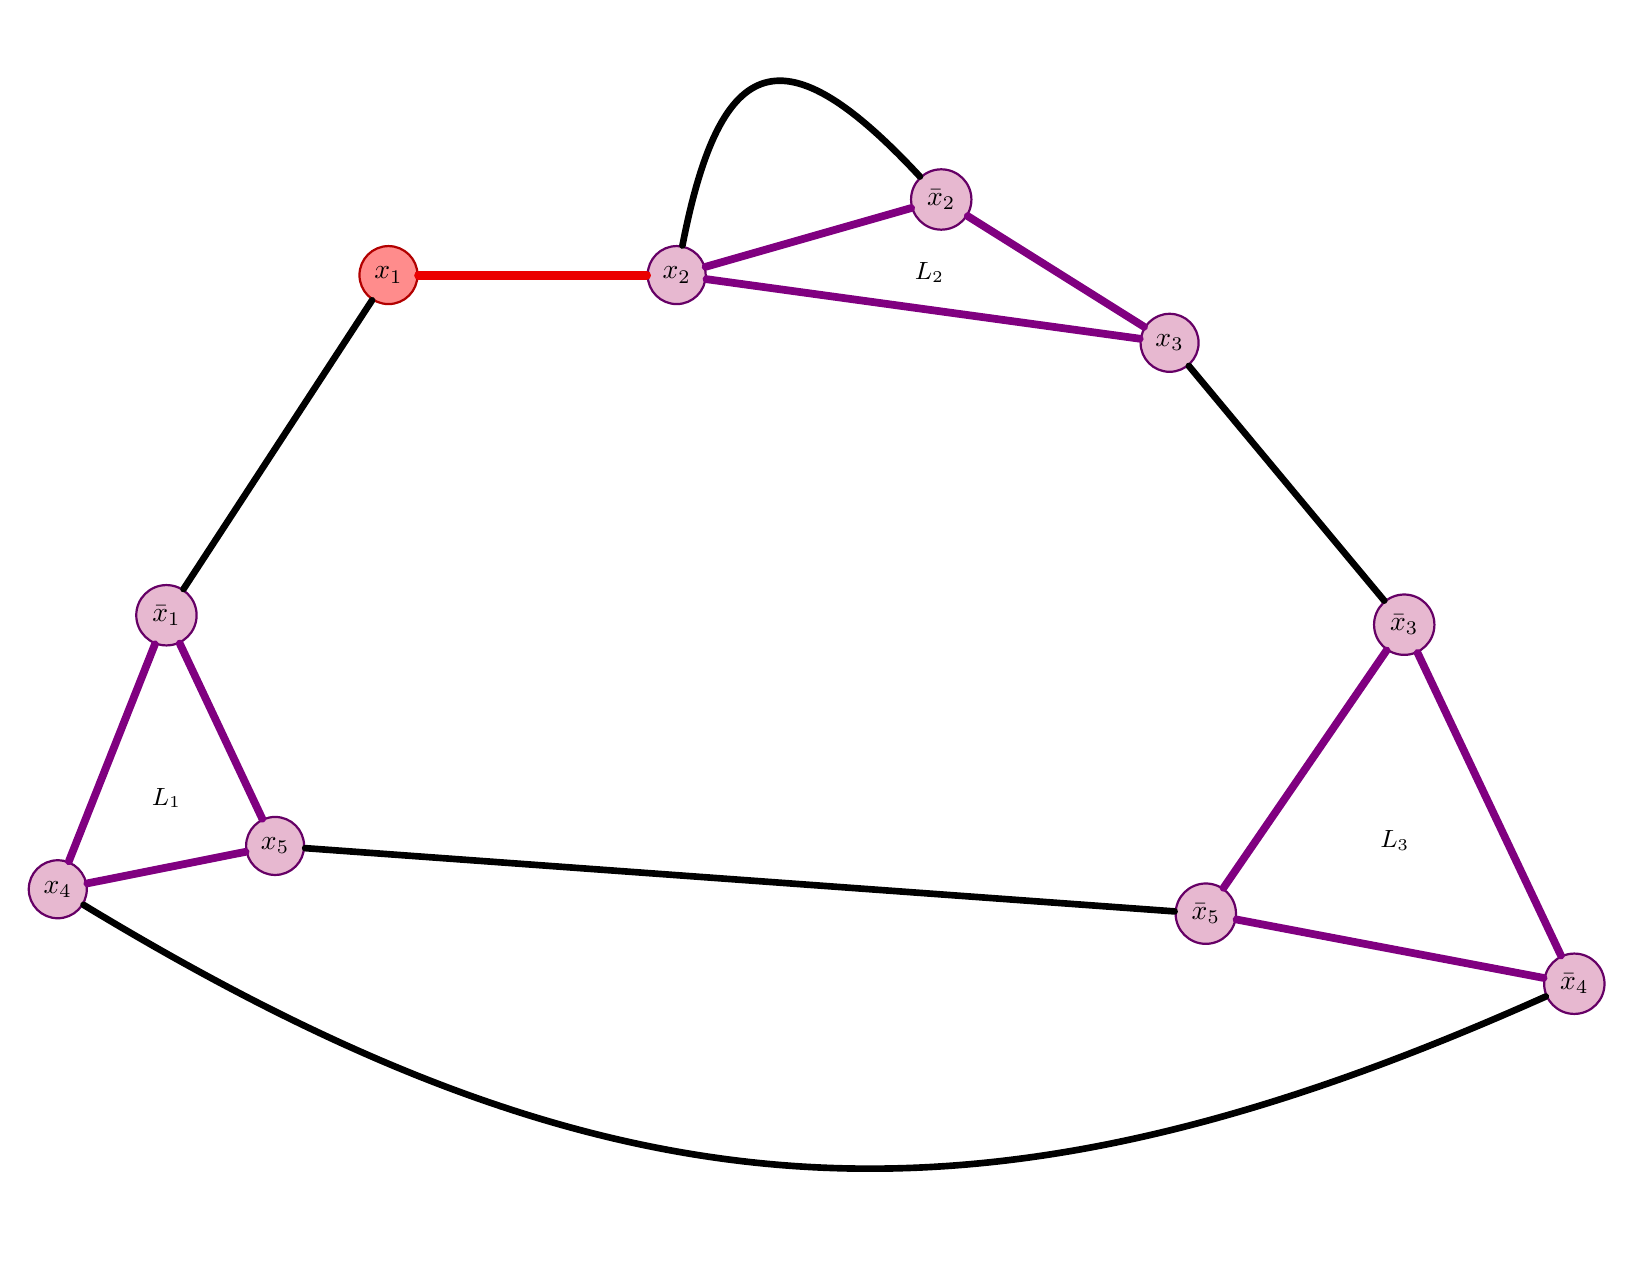
\begin{tikzpicture}[
  lbl/.style={font=\small, inner sep=1pt},
  redv/.style={circle, draw=red!70!black, line width=0.8pt, fill=red!45, minimum size=7mm},
  purpv/.style={circle, draw=violet!80!black, line width=0.8pt, fill=blue!12!purple!28, minimum size=7mm},
  purpleedge/.style={draw=violet, line width=2.8pt, line cap=round, line join=round},
  blackedge/.style={draw=black, line width=2.4pt, line cap=round},
  rededge/.style={draw=red!92!black, line width=3.2pt, line cap=round}
]

\node[redv] (nx1) at (-3.84, 6.18) {$x_{1}$};
\node[purpv] (nb1) at (-6.66, 1.86) {$\bar{x}_{1}$};
\node[purpv] (nx2) at (-0.18, 6.18) {$x_{2}$};
\node[purpv] (nb2) at (3.18, 7.14) {$\bar{x}_{2}$};
\node[purpv] (nx3) at (6.08, 5.32) {$x_{3}$};
\node[purpv] (nb3) at (9.06, 1.74) {$\bar{x}_{3}$};
\node[purpv] (nx4) at (-8.04, -1.62) {$x_{4}$};
\node[purpv] (nb4) at (11.22, -2.82) {$\bar{x}_{4}$};
\node[purpv] (nx5) at (-5.28, -1.07) {$x_{5}$};
\node[purpv] (nb5) at (6.54, -1.93) {$\bar{x}_{5}$};
\draw[purpleedge] (nb1) -- (nx4);
\draw[purpleedge] (nb1) -- (nx5);
\draw[purpleedge] (nx4) -- (nx5);
\draw[purpleedge] (nx2) -- (nb2);
\draw[purpleedge] (nx2) -- (nx3);
\draw[purpleedge] (nb2) -- (nx3);
\draw[purpleedge] (nb3) -- (nb4);
\draw[purpleedge] (nb3) -- (nb5);
\draw[purpleedge] (nb4) -- (nb5);
\draw[blackedge] (nx1) -- (nb1);
\draw[blackedge] (nx2) .. controls (0.38,9.05) and (1.19,9.28) .. (nb2);
\draw[blackedge] (nx3) -- (nb3);
\draw[blackedge] (nx4) .. controls (-0.96,-5.91) and (3.66,-6.20) .. (nb4);
\draw[blackedge] (nx5) -- (nb5);
\draw[rededge] (nx1) -- (nx2);
\node[lbl] at (-6.66, -0.46) {$L_1$};
\node[lbl] at (3.03, 6.21) {$L_2$};
\node[lbl] at (8.94, -1.00) {$L_3$};

\end{tikzpicture}%
}%

\end{center}
\medskip
\subsection*{Class 10 (IX)}
\noindent Representative of this ep-isomorphism class.\\
\noindent Distinguished indices:\\ $\{33, 34, 35, 40, 92, 94, 96, 99, 142, 143, 147, 148, 212, 215, 218, 219, 222, 226, 227, 230, 233, 234, 235, 240\}$, $24$ total.
\begin{center}
\resizebox{\linewidth}{!}{%
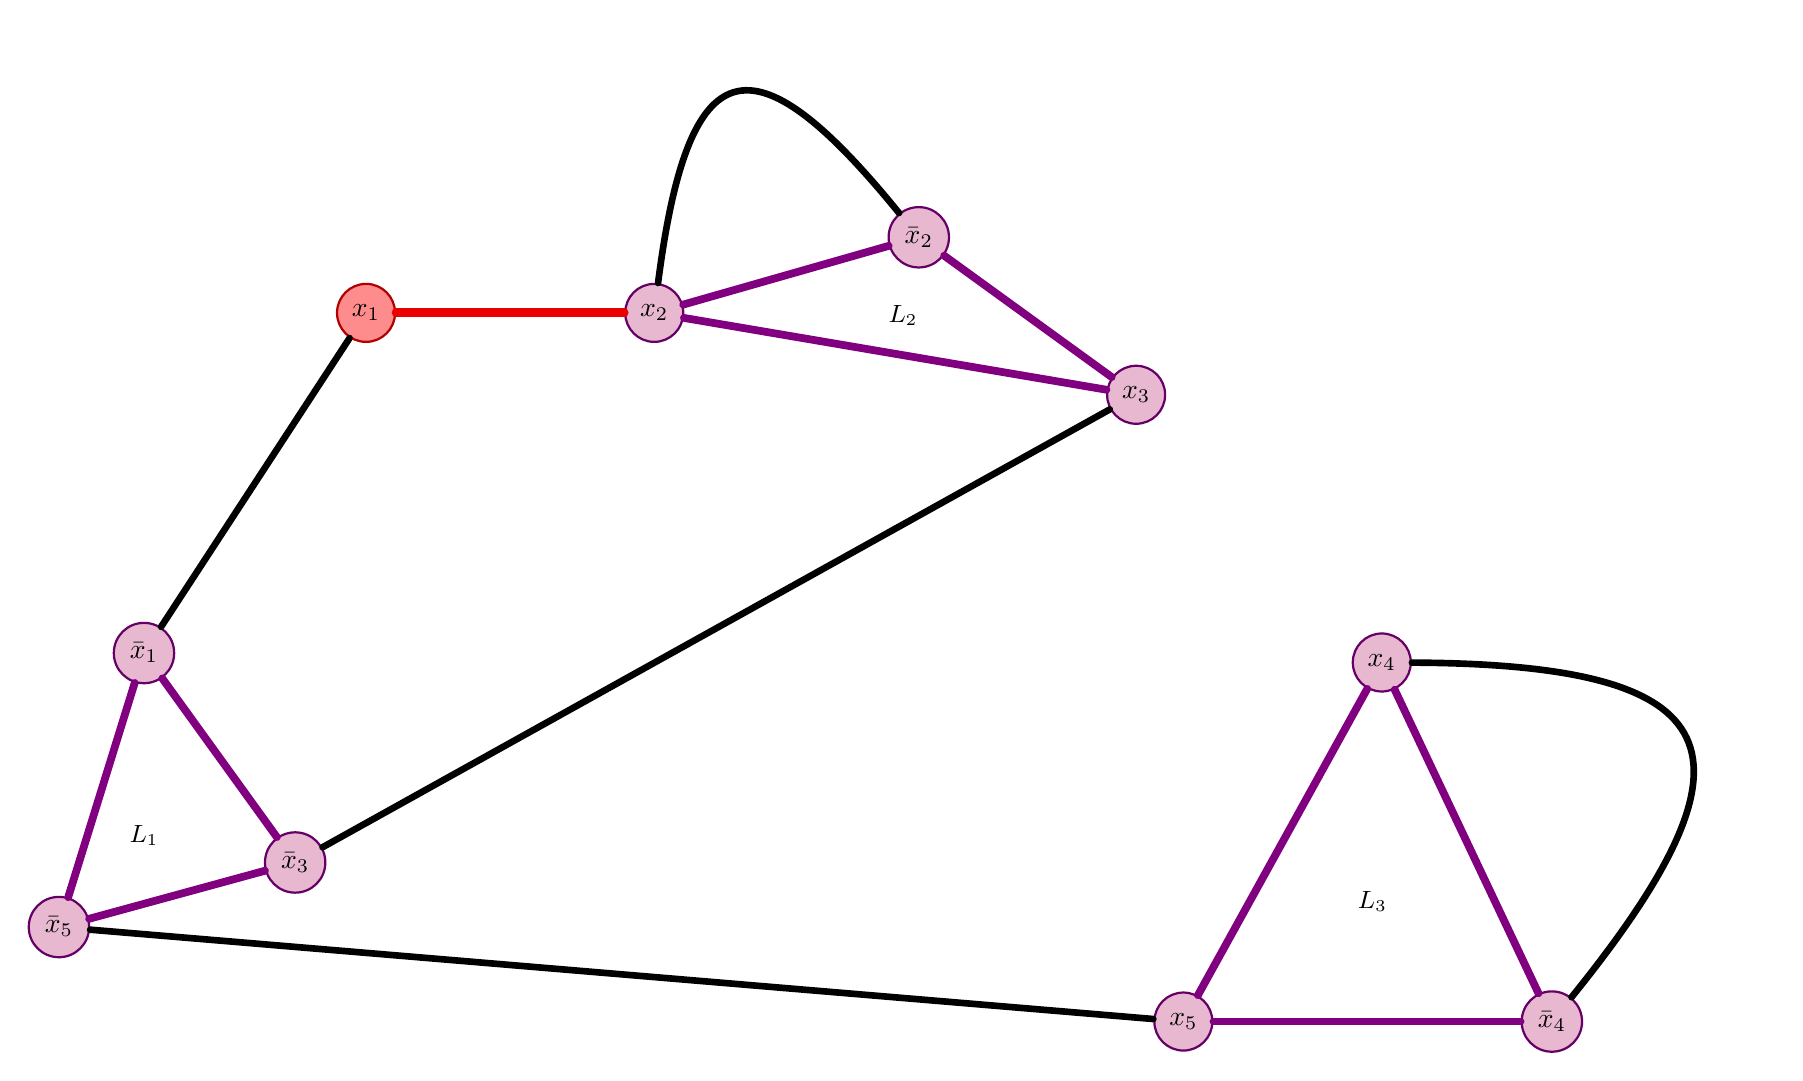
\begin{tikzpicture}[
  lbl/.style={font=\small, inner sep=1pt},
  redv/.style={circle, draw=red!70!black, line width=0.8pt, fill=red!45, minimum size=7mm},
  purpv/.style={circle, draw=violet!80!black, line width=0.8pt, fill=blue!12!purple!28, minimum size=7mm},
  purpleedge/.style={draw=violet, line width=2.8pt, line cap=round, line join=round},
  blackedge/.style={draw=black, line width=2.4pt, line cap=round},
  rededge/.style={draw=red!92!black, line width=3.2pt, line cap=round}
]

\node[redv] (nx1) at (-3.84, 6.18) {$x_{1}$};
\node[purpv] (nb1) at (-6.66, 1.86) {$\bar{x}_{1}$};
\node[purpv] (nx2) at (-0.18, 6.18) {$x_{2}$};
\node[purpv] (nb2) at (3.18, 7.14) {$\bar{x}_{2}$};
\node[purpv] (nx3) at (5.94, 5.14) {$x_{3}$};
\node[purpv] (nb3) at (-4.74, -0.80) {$\bar{x}_{3}$};
\node[purpv] (nx4) at (9.06, 1.74) {$x_{4}$};
\node[purpv] (nb4) at (11.22, -2.82) {$\bar{x}_{4}$};
\node[purpv] (nx5) at (6.54, -2.82) {$x_{5}$};
\node[purpv] (nb5) at (-7.74, -1.62) {$\bar{x}_{5}$};
\draw[purpleedge] (nb1) -- (nb3);
\draw[purpleedge] (nb1) -- (nb5);
\draw[purpleedge] (nb3) -- (nb5);
\draw[purpleedge] (nx2) -- (nb2);
\draw[purpleedge] (nx2) -- (nx3);
\draw[purpleedge] (nb2) -- (nx3);
\draw[purpleedge] (nx4) -- (nb4);
\draw[purpleedge] (nx4) -- (nx5);
\draw[purpleedge] (nb4) -- (nx5);
\draw[blackedge] (nx1) -- (nb1);
\draw[blackedge] (nx2) .. controls (0.25,9.53) and (1.05,9.76) .. (nb2);
\draw[blackedge] (nx3) -- (nb3);
\draw[blackedge] (nx4) .. controls (13.50,1.72) and (14.01,0.63) .. (nb4);
\draw[blackedge] (nx5) -- (nb5);
\draw[rededge] (nx1) -- (nx2);
\node[lbl] at (-6.66, -0.46) {$L_1$};
\node[lbl] at (2.98, 6.15) {$L_2$};
\node[lbl] at (8.94, -1.30) {$L_3$};

\end{tikzpicture}%
}%

\end{center}
\medskip
\subsection*{Class 11 (XIII)}
\noindent Representative of this ep-isomorphism class.\\
\noindent Distinguished indices: $\{36, 38, 95, 98, 145, 149, 213, 217, 223, 228, 236, 238\}$, $12$ total.
\begin{center}
\resizebox{\linewidth}{!}{%
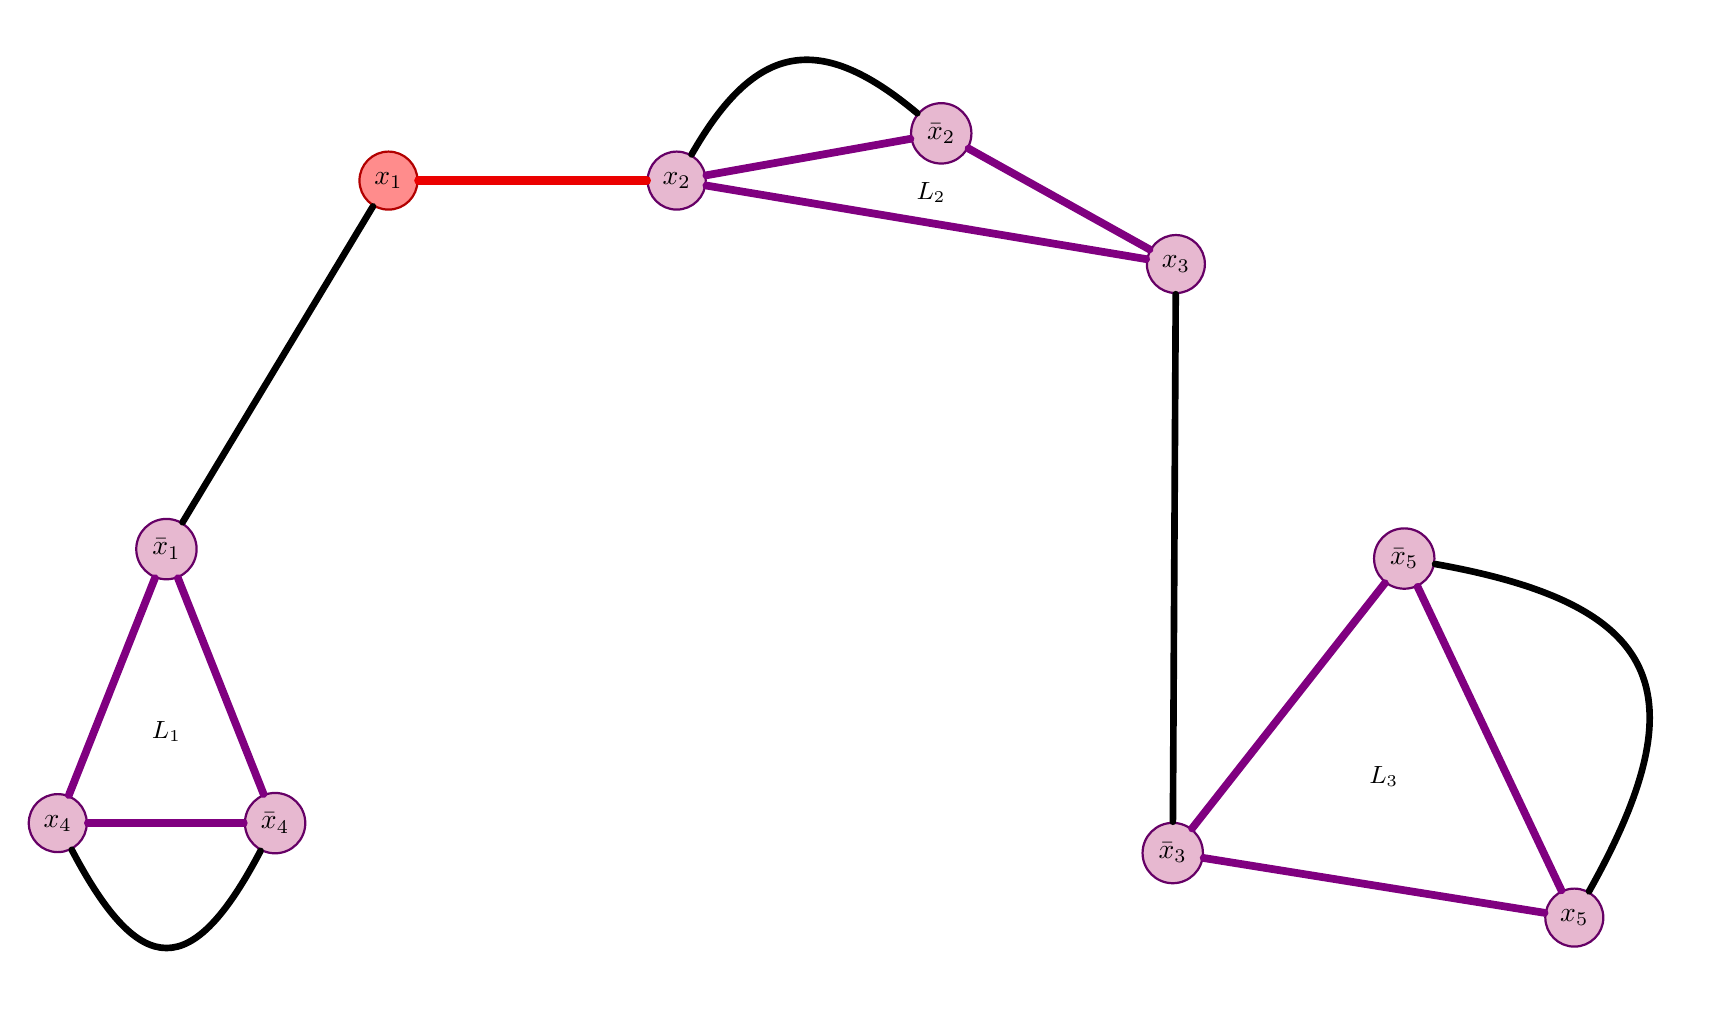
\begin{tikzpicture}[
  lbl/.style={font=\small, inner sep=1pt},
  redv/.style={circle, draw=red!70!black, line width=0.8pt, fill=red!45, minimum size=7mm},
  purpv/.style={circle, draw=violet!80!black, line width=0.8pt, fill=blue!12!purple!28, minimum size=7mm},
  purpleedge/.style={draw=violet, line width=2.8pt, line cap=round, line join=round},
  blackedge/.style={draw=black, line width=2.4pt, line cap=round},
  rededge/.style={draw=red!92!black, line width=3.2pt, line cap=round}
]

\node[redv] (nx1) at (-3.84, 6.54) {$x_{1}$};
\node[purpv] (nb1) at (-6.66, 1.86) {$\bar{x}_{1}$};
\node[purpv] (nx2) at (-0.18, 6.54) {$x_{2}$};
\node[purpv] (nb2) at (3.18, 7.14) {$\bar{x}_{2}$};
\node[purpv] (nx3) at (6.16, 5.48) {$x_{3}$};
\node[purpv] (nb3) at (6.12, -2.00) {$\bar{x}_{3}$};
\node[purpv] (nx4) at (-8.04, -1.62) {$x_{4}$};
\node[purpv] (nb4) at (-5.28, -1.62) {$\bar{x}_{4}$};
\node[purpv] (nx5) at (11.22, -2.82) {$x_{5}$};
\node[purpv] (nb5) at (9.06, 1.74) {$\bar{x}_{5}$};
\draw[purpleedge] (nb1) -- (nx4);
\draw[purpleedge] (nb1) -- (nb4);
\draw[purpleedge] (nx4) -- (nb4);
\draw[purpleedge] (nx2) -- (nb2);
\draw[purpleedge] (nx2) -- (nx3);
\draw[purpleedge] (nb2) -- (nx3);
\draw[purpleedge] (nb3) -- (nx5);
\draw[purpleedge] (nb3) -- (nb5);
\draw[purpleedge] (nx5) -- (nb5);
\draw[blackedge] (nx1) -- (nb1);
\draw[blackedge] (nx2) .. controls (0.82,8.29) and (1.63,8.44) .. (nb2);
\draw[blackedge] (nx3) -- (nb3);
\draw[blackedge] (nx4) .. controls (-6.99,-3.62) and (-6.33,-3.62) .. (nb4);
\draw[blackedge] (nx5) .. controls (12.84,0.07) and (12.32,1.16) .. (nb5);
\draw[rededge] (nx1) -- (nx2);
\node[lbl] at (-6.66, -0.46) {$L_1$};
\node[lbl] at (3.05, 6.39) {$L_2$};
\node[lbl] at (8.80, -1.03) {$L_3$};

\end{tikzpicture}%
}%

\end{center}
\medskip
\subsection*{Class 12 (V)}
\noindent Representative of this ep-isomorphism class.\\
\noindent Distinguished indices: $\{41, 42, 47, 49, 111, 112, 117, 119, 171, 172, 177, 179\}$, $12$ total.
\begin{center}
\resizebox{\linewidth}{!}{%
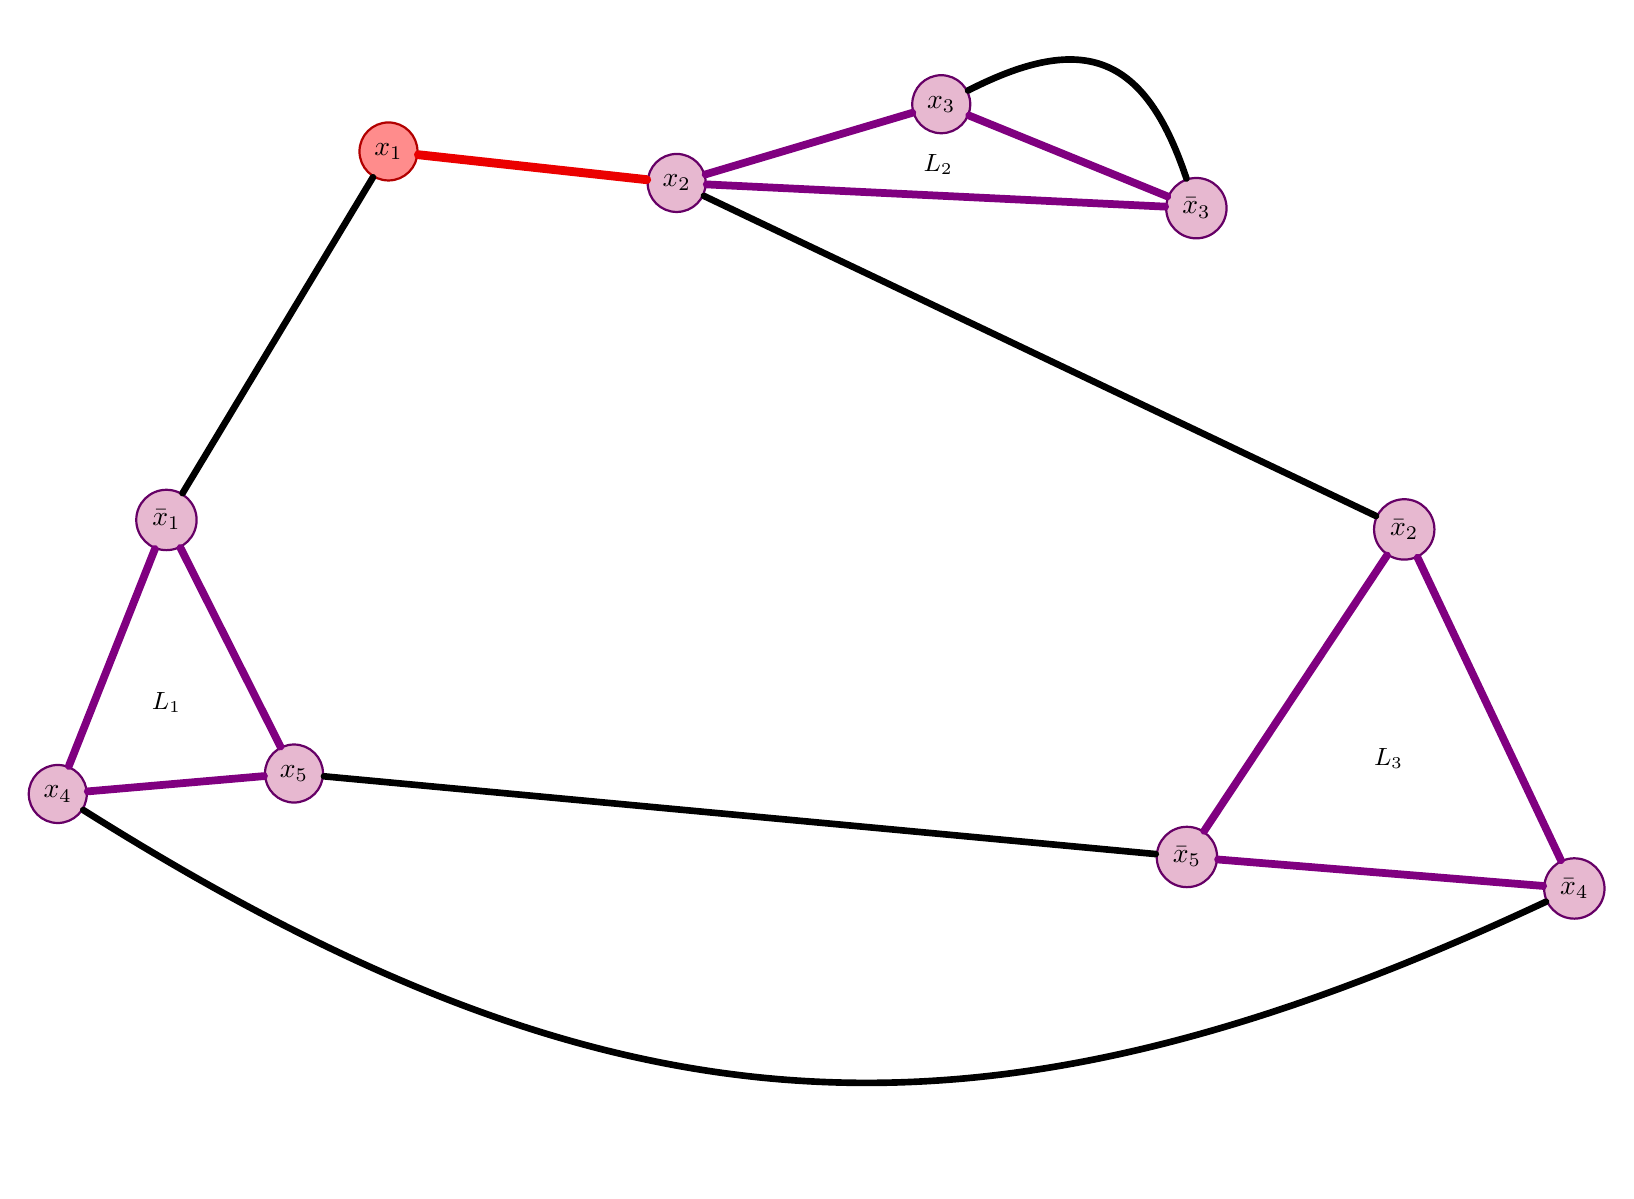
\begin{tikzpicture}[
  lbl/.style={font=\small, inner sep=1pt},
  redv/.style={circle, draw=red!70!black, line width=0.8pt, fill=red!45, minimum size=7mm},
  purpv/.style={circle, draw=violet!80!black, line width=0.8pt, fill=blue!12!purple!28, minimum size=7mm},
  purpleedge/.style={draw=violet, line width=2.8pt, line cap=round, line join=round},
  blackedge/.style={draw=black, line width=2.4pt, line cap=round},
  rededge/.style={draw=red!92!black, line width=3.2pt, line cap=round}
]

\node[redv] (nx1) at (-3.84, 6.54) {$x_{1}$};
\node[purpv] (nb1) at (-6.66, 1.86) {$\bar{x}_{1}$};
\node[purpv] (nx2) at (-0.18, 6.14) {$x_{2}$};
\node[purpv] (nb2) at (9.06, 1.74) {$\bar{x}_{2}$};
\node[purpv] (nx3) at (3.18, 7.14) {$x_{3}$};
\node[purpv] (nb3) at (6.42, 5.82) {$\bar{x}_{3}$};
\node[purpv] (nx4) at (-8.04, -1.62) {$x_{4}$};
\node[purpv] (nb4) at (11.22, -2.82) {$\bar{x}_{4}$};
\node[purpv] (nx5) at (-5.04, -1.36) {$x_{5}$};
\node[purpv] (nb5) at (6.30, -2.42) {$\bar{x}_{5}$};
\draw[purpleedge] (nb1) -- (nx4);
\draw[purpleedge] (nb1) -- (nx5);
\draw[purpleedge] (nx4) -- (nx5);
\draw[purpleedge] (nx2) -- (nx3);
\draw[purpleedge] (nx2) -- (nb3);
\draw[purpleedge] (nx3) -- (nb3);
\draw[purpleedge] (nb2) -- (nb4);
\draw[purpleedge] (nb2) -- (nb5);
\draw[purpleedge] (nb4) -- (nb5);
\draw[blackedge] (nx1) -- (nb1);
\draw[blackedge] (nx2) -- (nb2);
\draw[blackedge] (nx3) .. controls (5.00,8.07) and (5.77,7.76) .. (nb3);
\draw[blackedge] (nx4) .. controls (-0.97,-6.07) and (3.65,-6.36) .. (nb4);
\draw[blackedge] (nx5) -- (nb5);
\draw[rededge] (nx1) -- (nx2);
\node[lbl] at (-6.66, -0.46) {$L_1$};
\node[lbl] at (3.14, 6.37) {$L_2$};
\node[lbl] at (8.86, -1.17) {$L_3$};

\end{tikzpicture}%
}%

\end{center}
\medskip
\subsection*{Class 13 (XI)}
\noindent Representative of this ep-isomorphism class.\\
\noindent Distinguished indices: $\{43, 44, 45, 50, 113, 114, 115, 120, 173, 174, 175, 180\}$, $12$ total.
\begin{center}
\resizebox{\linewidth}{!}{%
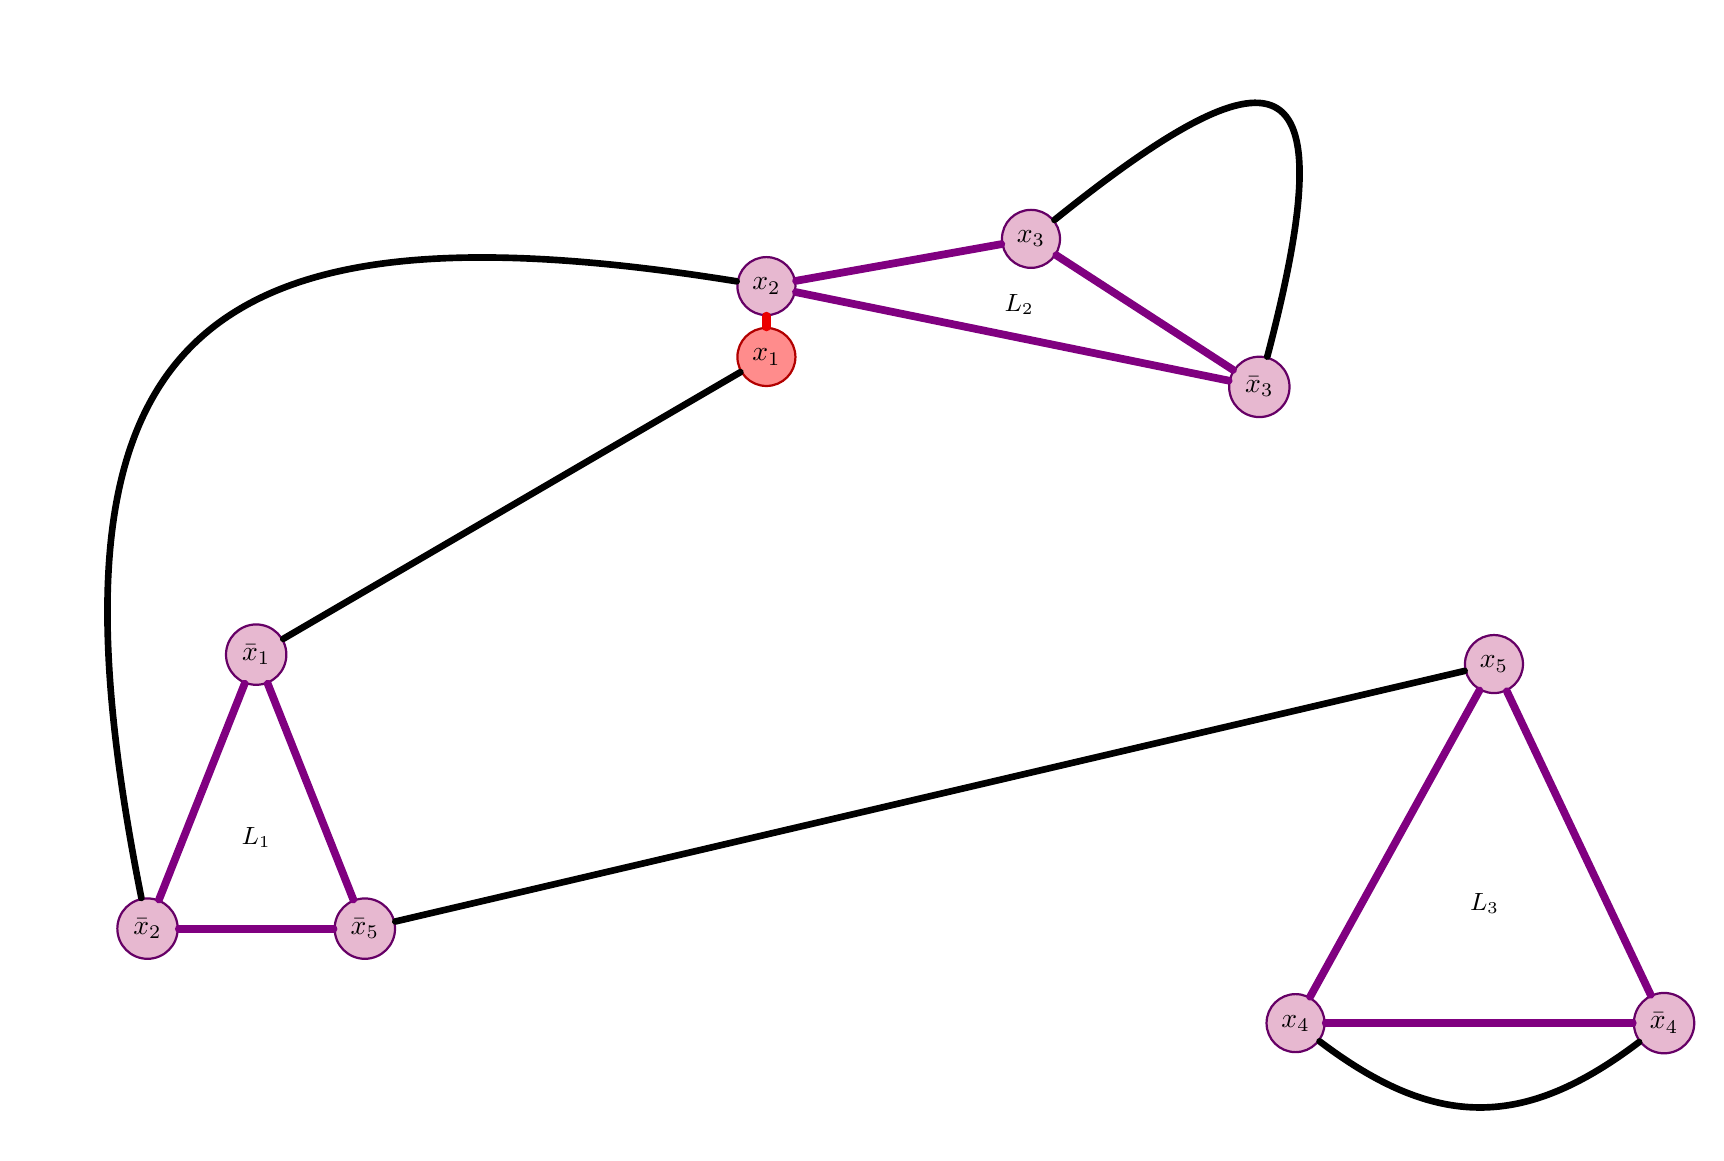
\begin{tikzpicture}[
  lbl/.style={font=\small, inner sep=1pt},
  redv/.style={circle, draw=red!70!black, line width=0.8pt, fill=red!45, minimum size=7mm},
  purpv/.style={circle, draw=violet!80!black, line width=0.8pt, fill=blue!12!purple!28, minimum size=7mm},
  purpleedge/.style={draw=violet, line width=2.8pt, line cap=round, line join=round},
  blackedge/.style={draw=black, line width=2.4pt, line cap=round},
  rededge/.style={draw=red!92!black, line width=3.2pt, line cap=round}
]

\node[redv] (nx1) at (-0.18, 5.64) {$x_{1}$};
\node[purpv] (nb1) at (-6.66, 1.86) {$\bar{x}_{1}$};
\node[purpv] (nx2) at (-0.18, 6.54) {$x_{2}$};
\node[purpv] (nb2) at (-8.04, -1.62) {$\bar{x}_{2}$};
\node[purpv] (nx3) at (3.18, 7.14) {$x_{3}$};
\node[purpv] (nb3) at (6.08, 5.26) {$\bar{x}_{3}$};
\node[purpv] (nx4) at (6.54, -2.82) {$x_{4}$};
\node[purpv] (nb4) at (11.22, -2.82) {$\bar{x}_{4}$};
\node[purpv] (nx5) at (9.06, 1.74) {$x_{5}$};
\node[purpv] (nb5) at (-5.28, -1.62) {$\bar{x}_{5}$};
\draw[purpleedge] (nb1) -- (nb2);
\draw[purpleedge] (nb1) -- (nb5);
\draw[purpleedge] (nb2) -- (nb5);
\draw[purpleedge] (nx2) -- (nx3);
\draw[purpleedge] (nx2) -- (nb3);
\draw[purpleedge] (nx3) -- (nb3);
\draw[purpleedge] (nx4) -- (nb4);
\draw[purpleedge] (nx4) -- (nx5);
\draw[purpleedge] (nb4) -- (nx5);
\draw[blackedge] (nx1) -- (nb1);
\draw[blackedge] (nx2) .. controls (-7.63,7.74) and (-9.52,5.78) .. (nb2);
\draw[blackedge] (nx3) .. controls (6.46,9.78) and (7.15,9.33) .. (nb3);
\draw[blackedge] (nx4) .. controls (8.32,-4.17) and (9.44,-4.17) .. (nb4);
\draw[blackedge] (nx5) -- (nb5);
\draw[rededge] (nx1) -- (nx2);
\node[lbl] at (-6.66, -0.46) {$L_1$};
\node[lbl] at (3.03, 6.31) {$L_2$};
\node[lbl] at (8.94, -1.30) {$L_3$};

\end{tikzpicture}%
}%

\end{center}
\medskip
\subsection*{Class 14 (XIV)}
\noindent Representative of this ep-isomorphism class.\\
\noindent Distinguished indices: $\{46, 48, 116, 118, 176, 178\}$, $6$ total.
\begin{center}
\resizebox{\linewidth}{!}{%
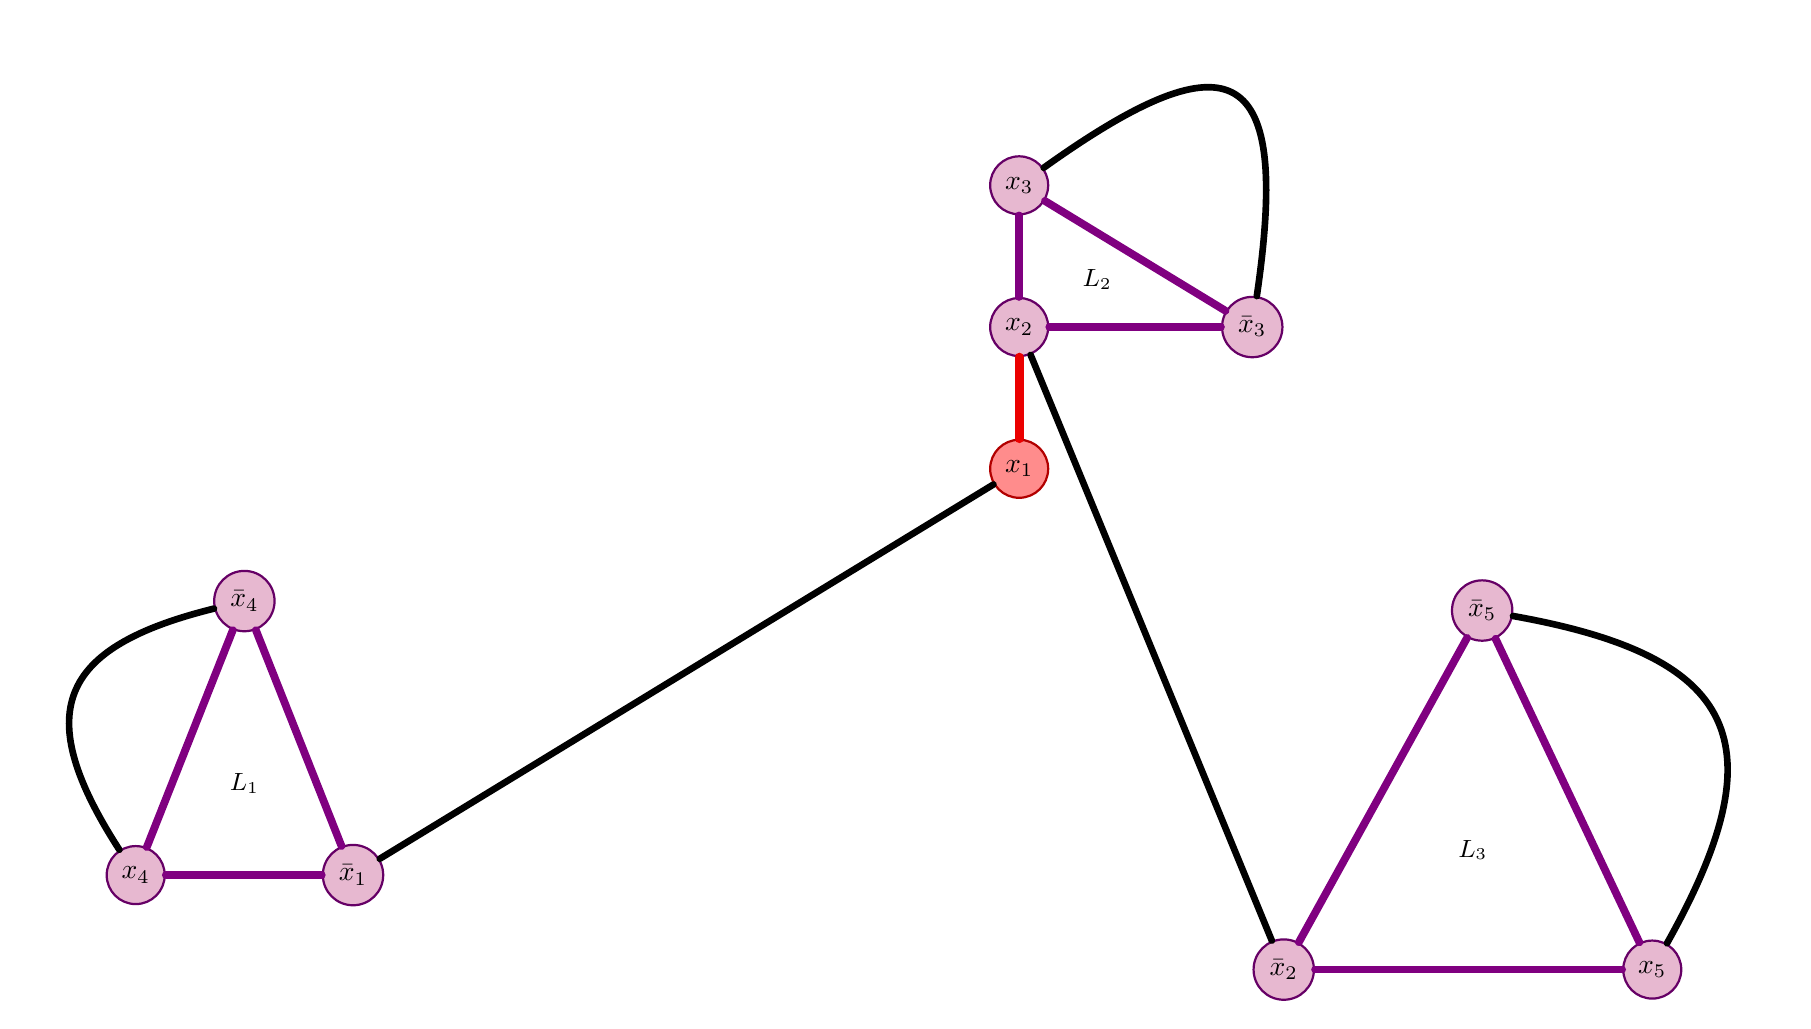
\begin{tikzpicture}[
  lbl/.style={font=\small, inner sep=1pt},
  redv/.style={circle, draw=red!70!black, line width=0.8pt, fill=red!45, minimum size=7mm},
  purpv/.style={circle, draw=violet!80!black, line width=0.8pt, fill=blue!12!purple!28, minimum size=7mm},
  purpleedge/.style={draw=violet, line width=2.8pt, line cap=round, line join=round},
  blackedge/.style={draw=black, line width=2.4pt, line cap=round},
  rededge/.style={draw=red!92!black, line width=3.2pt, line cap=round}
]

\node[redv] (nx1) at (3.18, 3.54) {$x_{1}$};
\node[purpv] (nb1) at (-5.28, -1.62) {$\bar{x}_{1}$};
\node[purpv] (nx2) at (3.18, 5.34) {$x_{2}$};
\node[purpv] (nb2) at (6.54, -2.82) {$\bar{x}_{2}$};
\node[purpv] (nx3) at (3.18, 7.14) {$x_{3}$};
\node[purpv] (nb3) at (6.14, 5.34) {$\bar{x}_{3}$};
\node[purpv] (nx4) at (-8.04, -1.62) {$x_{4}$};
\node[purpv] (nb4) at (-6.66, 1.86) {$\bar{x}_{4}$};
\node[purpv] (nx5) at (11.22, -2.82) {$x_{5}$};
\node[purpv] (nb5) at (9.06, 1.74) {$\bar{x}_{5}$};
\draw[purpleedge] (nb1) -- (nx4);
\draw[purpleedge] (nb1) -- (nb4);
\draw[purpleedge] (nx4) -- (nb4);
\draw[purpleedge] (nx2) -- (nx3);
\draw[purpleedge] (nx2) -- (nb3);
\draw[purpleedge] (nx3) -- (nb3);
\draw[purpleedge] (nb2) -- (nx5);
\draw[purpleedge] (nb2) -- (nb5);
\draw[purpleedge] (nx5) -- (nb5);
\draw[blackedge] (nx1) -- (nb1);
\draw[blackedge] (nx2) -- (nb2);
\draw[blackedge] (nx3) .. controls (5.92,9.10) and (6.63,8.67) .. (nb3);
\draw[blackedge] (nx4) .. controls (-9.37,0.44) and (-9.04,1.27) .. (nb4);
\draw[blackedge] (nx5) .. controls (12.84,0.07) and (12.32,1.16) .. (nb5);
\draw[rededge] (nx1) -- (nx2);
\node[lbl] at (-6.66, -0.46) {$L_1$};
\node[lbl] at (4.17, 5.94) {$L_2$};
\node[lbl] at (8.94, -1.30) {$L_3$};

\end{tikzpicture}%
}%

\end{center}
\medskip

\section[Output of Step 2 and Step 3 for the seed ltt structure]{Output of Step 2 and Step 3 for the seed ltt structure (Tasks~\ref{t:Step2} and~\ref{t:Step3})}

\noindent\textit{Regenerating this appendix.} Run \texttt{python generate\_step2\_appendix\_tex.py} and \texttt{python generate\_step3\_appendix\_tex.py} from the repository root; they fill \texttt{step2\_seed\_appendix\_generated.tex} and \texttt{step3\_seed\_appendix\_generated.tex} with formatted \LaTeX{} (matching \texttt{run\_step2\_seed.py} and \texttt{run\_step3\_seed.py}).

\subsection*{Seed \emph{ltt} structure $G$}
\begin{description}[style=nextline, font=\normalfont\bfseries]
\item[Red vertex] $\displaystyle x_{1}$.
\item[Red edge] $\displaystyle \{x_{1},\,\bar{x}_{5}\}$.
\item[Purple edges ($9$)]\mbox{}\\
$P_{1}: \{x_{2},\,x_{4}\},\; \{x_{2},\,x_{5}\},\; \{x_{4},\,x_{5}\}$\\
$P_{2}: \{x_{3},\,\bar{x}_{1}\},\; \{x_{3},\,\bar{x}_{2}\},\; \{\bar{x}_{1},\,\bar{x}_{2}\}$\\
$P_{3}: \{\bar{x}_{3},\,\bar{x}_{4}\},\; \{\bar{x}_{3},\,\bar{x}_{5}\},\; \{\bar{x}_{4},\,\bar{x}_{5}\}$
\item[Black edges ($5$)] $\displaystyle \{x_{1},\,\bar{x}_{1}\},\; \{x_{2},\,\bar{x}_{2}\},\; \{x_{3},\,\bar{x}_{3}\},\; \{x_{4},\,\bar{x}_{4}\},\; \{x_{5},\,\bar{x}_{5}\}$.
\end{description}

\subsection*{Step $2$ parameters}
$d_r = x_{1}$, $d_p = \bar{x}_{5}$ (purple endpoint of the red edge).\par\smallskip
\noindent\textit{Prompt alignment:} rule~(j;a) specifies red vertex $d_r$, red edge $\{d_r,\bar{d}_j\}$, and purple edges exactly as in $G$; rule~(j;b) adds purple edges from colored neighbors of $d_j$ and inherits only purple edges not incident to $d_j$ (see \texttt{ltt\_structures.terminal\_ga\_step2} and \texttt{ltt\_structures.terminal\_gb\_step2}). Directed-edge labels use $(d_r,d_j)$.

Membership in $\mathrm{PLTT}$ uses ep-isomorphism to one of the $270$ distinguished graphs (same enumeration as \texttt{list\_admissible\_ltt\_classes.py}).\par\smallskip

\subsection*{Terminal graphs $\mathrm{terminal}(G)=\{G_{1a},G_{1b},G_{2a},G_{2b}\}$}
\begin{enumerate}[label=\textbf{\arabic*.}, leftmargin=*]
\item $G_{1a}$: directed edge label $x_{1} \to \bar{x}_{3}\,x_{1}$, (rule 2a: $d_r \to d_j\, d_r$). \textbf{retained} (in $\mathrm{PLTT}$).
\begin{description}[style=nextline, font=\normalfont\bfseries]
\item[Red vertex] $\displaystyle x_{1}$.
\item[Red edge] $\displaystyle \{x_{1},\,x_{3}\}$.
\item[Purple edges ($9$)]\mbox{}\\
$P_{1}: \{x_{2},\,x_{4}\},\; \{x_{2},\,x_{5}\},\; \{x_{4},\,x_{5}\}$\\
$P_{2}: \{x_{3},\,\bar{x}_{1}\},\; \{x_{3},\,\bar{x}_{2}\},\; \{\bar{x}_{1},\,\bar{x}_{2}\}$\\
$P_{3}: \{\bar{x}_{3},\,\bar{x}_{4}\},\; \{\bar{x}_{3},\,\bar{x}_{5}\},\; \{\bar{x}_{4},\,\bar{x}_{5}\}$
\item[Black edges ($5$)] $\displaystyle \{x_{1},\,\bar{x}_{1}\},\; \{x_{2},\,\bar{x}_{2}\},\; \{x_{3},\,\bar{x}_{3}\},\; \{x_{4},\,\bar{x}_{4}\},\; \{x_{5},\,\bar{x}_{5}\}$.
\end{description}
\item $G_{1b}$: directed edge label $\bar{x}_{3} \to x_{1}\,\bar{x}_{3}$, (rule 2b: $d_j \to d_r\, d_j$). \textbf{retained} (in $\mathrm{PLTT}$).
\begin{description}[style=nextline, font=\normalfont\bfseries]
\item[Red vertex] $\displaystyle \bar{x}_{3}$.
\item[Red edge] $\displaystyle \{\bar{x}_{1},\,\bar{x}_{3}\}$.
\item[Purple edges ($9$)]\mbox{}\\
$P_{1}: \{x_{1},\,\bar{x}_{4}\},\; \{x_{1},\,\bar{x}_{5}\},\; \{\bar{x}_{4},\,\bar{x}_{5}\}$\\
$P_{2}: \{x_{2},\,x_{4}\},\; \{x_{2},\,x_{5}\},\; \{x_{4},\,x_{5}\}$\\
$P_{3}: \{x_{3},\,\bar{x}_{1}\},\; \{x_{3},\,\bar{x}_{2}\},\; \{\bar{x}_{1},\,\bar{x}_{2}\}$
\item[Black edges ($5$)] $\displaystyle \{x_{1},\,\bar{x}_{1}\},\; \{x_{2},\,\bar{x}_{2}\},\; \{x_{3},\,\bar{x}_{3}\},\; \{x_{4},\,\bar{x}_{4}\},\; \{x_{5},\,\bar{x}_{5}\}$.
\end{description}
\item $G_{2a}$: directed edge label $x_{1} \to \bar{x}_{4}\,x_{1}$, (rule 2a: $d_r \to d_j\, d_r$). \textbf{retained} (in $\mathrm{PLTT}$).
\begin{description}[style=nextline, font=\normalfont\bfseries]
\item[Red vertex] $\displaystyle x_{1}$.
\item[Red edge] $\displaystyle \{x_{1},\,x_{4}\}$.
\item[Purple edges ($9$)]\mbox{}\\
$P_{1}: \{x_{2},\,x_{4}\},\; \{x_{2},\,x_{5}\},\; \{x_{4},\,x_{5}\}$\\
$P_{2}: \{x_{3},\,\bar{x}_{1}\},\; \{x_{3},\,\bar{x}_{2}\},\; \{\bar{x}_{1},\,\bar{x}_{2}\}$\\
$P_{3}: \{\bar{x}_{3},\,\bar{x}_{4}\},\; \{\bar{x}_{3},\,\bar{x}_{5}\},\; \{\bar{x}_{4},\,\bar{x}_{5}\}$
\item[Black edges ($5$)] $\displaystyle \{x_{1},\,\bar{x}_{1}\},\; \{x_{2},\,\bar{x}_{2}\},\; \{x_{3},\,\bar{x}_{3}\},\; \{x_{4},\,\bar{x}_{4}\},\; \{x_{5},\,\bar{x}_{5}\}$.
\end{description}
\item $G_{2b}$: directed edge label $\bar{x}_{4} \to x_{1}\,\bar{x}_{4}$, (rule 2b: $d_j \to d_r\, d_j$). \textbf{retained} (in $\mathrm{PLTT}$).
\begin{description}[style=nextline, font=\normalfont\bfseries]
\item[Red vertex] $\displaystyle \bar{x}_{4}$.
\item[Red edge] $\displaystyle \{\bar{x}_{1},\,\bar{x}_{4}\}$.
\item[Purple edges ($9$)]\mbox{}\\
$P_{1}: \{x_{1},\,\bar{x}_{3}\},\; \{x_{1},\,\bar{x}_{5}\},\; \{\bar{x}_{3},\,\bar{x}_{5}\}$\\
$P_{2}: \{x_{2},\,x_{4}\},\; \{x_{2},\,x_{5}\},\; \{x_{4},\,x_{5}\}$\\
$P_{3}: \{x_{3},\,\bar{x}_{1}\},\; \{x_{3},\,\bar{x}_{2}\},\; \{\bar{x}_{1},\,\bar{x}_{2}\}$
\item[Black edges ($5$)] $\displaystyle \{x_{1},\,\bar{x}_{1}\},\; \{x_{2},\,\bar{x}_{2}\},\; \{x_{3},\,\bar{x}_{3}\},\; \{x_{4},\,\bar{x}_{4}\},\; \{x_{5},\,\bar{x}_{5}\}$.
\end{description}
\end{enumerate}

\subsection*{Step $3$ on seed output (Task~\ref{t:Step3})}
\noindent Starting from Step~1 initialization $\mathrm{GRAPHS}=\{G\}$, $\mathrm{graphs}_{1}=\{G\}$, $\mathrm{boxes}=\{\mathrm{graphs}_{1}\}$, $\mathrm{GRAPHS}_{1}=\{G\}$, apply Step~$3$ in the Step~$2$ order $\{G_{1a},G_{1b},G_{2a},G_{2b}\}$.

\begin{enumerate}[label=\textbf{\arabic*.}, leftmargin=*]
\item $G_{1a}$: new ep-isomorphism class; add $G_{1a}$ to $\mathrm{GRAPHS}$ and preAUT, create $\mathrm{graphs}_{2}=\{G_{1a}\}$, add $G_{1a}$ to $\mathrm{GRAPHS}_{2}$, and add edge $G \to G_{1a}$ with label $x_{1} \to \bar{x}_{3}\,x_{1}$.
\begin{description}[style=nextline, font=\normalfont\bfseries]
\item[Red vertex] $\displaystyle x_{1}$.
\item[Red edge] $\displaystyle \{x_{1},\,x_{3}\}$.
\item[Purple edges ($9$)]\mbox{}\\
$P_{1}: \{x_{2},\,x_{4}\},\; \{x_{2},\,x_{5}\},\; \{x_{4},\,x_{5}\}$\\
$P_{2}: \{x_{3},\,\bar{x}_{1}\},\; \{x_{3},\,\bar{x}_{2}\},\; \{\bar{x}_{1},\,\bar{x}_{2}\}$\\
$P_{3}: \{\bar{x}_{3},\,\bar{x}_{4}\},\; \{\bar{x}_{3},\,\bar{x}_{5}\},\; \{\bar{x}_{4},\,\bar{x}_{5}\}$
\item[Black edges ($5$)] $\displaystyle \{x_{1},\,\bar{x}_{1}\},\; \{x_{2},\,\bar{x}_{2}\},\; \{x_{3},\,\bar{x}_{3}\},\; \{x_{4},\,\bar{x}_{4}\},\; \{x_{5},\,\bar{x}_{5}\}$.
\end{description}
\item $G_{1b}$: ep-isomorphic to $G_{1a}$ (box $\mathrm{graphs}_{2}$), not equal; add $G_{1b}$ to $\mathrm{GRAPHS}$ and $\mathrm{graphs}_{2}$, and add permutation edge $G_{1b} \xrightarrow{\varphi} G_{1a}$ with $\varphi=x_{1} \mapsto \bar{x}_{3},\; x_{2} \mapsto x_{2},\; x_{3} \mapsto \bar{x}_{1},\; x_{4} \mapsto x_{4},\; x_{5} \mapsto x_{5}$.
\begin{description}[style=nextline, font=\normalfont\bfseries]
\item[Red vertex] $\displaystyle \bar{x}_{3}$.
\item[Red edge] $\displaystyle \{\bar{x}_{1},\,\bar{x}_{3}\}$.
\item[Purple edges ($9$)]\mbox{}\\
$P_{1}: \{x_{1},\,\bar{x}_{4}\},\; \{x_{1},\,\bar{x}_{5}\},\; \{\bar{x}_{4},\,\bar{x}_{5}\}$\\
$P_{2}: \{x_{2},\,x_{4}\},\; \{x_{2},\,x_{5}\},\; \{x_{4},\,x_{5}\}$\\
$P_{3}: \{x_{3},\,\bar{x}_{1}\},\; \{x_{3},\,\bar{x}_{2}\},\; \{\bar{x}_{1},\,\bar{x}_{2}\}$
\item[Black edges ($5$)] $\displaystyle \{x_{1},\,\bar{x}_{1}\},\; \{x_{2},\,\bar{x}_{2}\},\; \{x_{3},\,\bar{x}_{3}\},\; \{x_{4},\,\bar{x}_{4}\},\; \{x_{5},\,\bar{x}_{5}\}$.
\end{description}
\item $G_{2a}$: ep-isomorphic to $G$ (box $\mathrm{graphs}_{1}$), not equal; add $G_{2a}$ to $\mathrm{GRAPHS}$ and $\mathrm{graphs}_{1}$, and add permutation edge $G_{2a} \xrightarrow{\varphi} G$ with $\varphi=x_{1} \mapsto x_{1},\; x_{2} \mapsto \bar{x}_{3},\; x_{3} \mapsto \bar{x}_{2},\; x_{4} \mapsto \bar{x}_{5},\; x_{5} \mapsto \bar{x}_{4}$.
\begin{description}[style=nextline, font=\normalfont\bfseries]
\item[Red vertex] $\displaystyle x_{1}$.
\item[Red edge] $\displaystyle \{x_{1},\,x_{4}\}$.
\item[Purple edges ($9$)]\mbox{}\\
$P_{1}: \{x_{2},\,x_{4}\},\; \{x_{2},\,x_{5}\},\; \{x_{4},\,x_{5}\}$\\
$P_{2}: \{x_{3},\,\bar{x}_{1}\},\; \{x_{3},\,\bar{x}_{2}\},\; \{\bar{x}_{1},\,\bar{x}_{2}\}$\\
$P_{3}: \{\bar{x}_{3},\,\bar{x}_{4}\},\; \{\bar{x}_{3},\,\bar{x}_{5}\},\; \{\bar{x}_{4},\,\bar{x}_{5}\}$
\item[Black edges ($5$)] $\displaystyle \{x_{1},\,\bar{x}_{1}\},\; \{x_{2},\,\bar{x}_{2}\},\; \{x_{3},\,\bar{x}_{3}\},\; \{x_{4},\,\bar{x}_{4}\},\; \{x_{5},\,\bar{x}_{5}\}$.
\end{description}
\item $G_{2b}$: ep-isomorphic to $G$ (box $\mathrm{graphs}_{1}$), not equal; add $G_{2b}$ to $\mathrm{GRAPHS}$ and $\mathrm{graphs}_{1}$, and add permutation edge $G_{2b} \xrightarrow{\varphi} G$ with $\varphi=x_{1} \mapsto x_{5},\; x_{2} \mapsto x_{3},\; x_{3} \mapsto \bar{x}_{4},\; x_{4} \mapsto \bar{x}_{1},\; x_{5} \mapsto \bar{x}_{2}$.
\begin{description}[style=nextline, font=\normalfont\bfseries]
\item[Red vertex] $\displaystyle \bar{x}_{4}$.
\item[Red edge] $\displaystyle \{\bar{x}_{1},\,\bar{x}_{4}\}$.
\item[Purple edges ($9$)]\mbox{}\\
$P_{1}: \{x_{1},\,\bar{x}_{3}\},\; \{x_{1},\,\bar{x}_{5}\},\; \{\bar{x}_{3},\,\bar{x}_{5}\}$\\
$P_{2}: \{x_{2},\,x_{4}\},\; \{x_{2},\,x_{5}\},\; \{x_{4},\,x_{5}\}$\\
$P_{3}: \{x_{3},\,\bar{x}_{1}\},\; \{x_{3},\,\bar{x}_{2}\},\; \{\bar{x}_{1},\,\bar{x}_{2}\}$
\item[Black edges ($5$)] $\displaystyle \{x_{1},\,\bar{x}_{1}\},\; \{x_{2},\,\bar{x}_{2}\},\; \{x_{3},\,\bar{x}_{3}\},\; \{x_{4},\,\bar{x}_{4}\},\; \{x_{5},\,\bar{x}_{5}\}$.
\end{description}
\end{enumerate}

\paragraph{Outcome after Step $3$ for the seed.}
$\mathrm{GRAPHS}=\{G, G_{1a}, G_{1b}, G_{2a}, G_{2b}\}$.\\
$|\mathrm{boxes}|=2$, with:
\begin{itemize}[leftmargin=*]
\item $\mathrm{graphs}_{1}=\{G, G_{2a}, G_{2b}\}$.
\item $\mathrm{graphs}_{2}=\{G_{1a}, G_{1b}\}$.
\end{itemize}
$\mathrm{GRAPHS}_{2}=\{G_{1a}\}$.

\paragraph{preAUT edges added in this Step~$3$ pass.}
\begin{itemize}[leftmargin=*]
\item $G \xrightarrow{x_{1} \to \bar{x}_{3}\,x_{1}} G_{1a}$.
\item $G_{1b} \xrightarrow{\varphi} G_{1a}$ with $\varphi=x_{1} \mapsto \bar{x}_{3},\; x_{2} \mapsto x_{2},\; x_{3} \mapsto \bar{x}_{1},\; x_{4} \mapsto x_{4},\; x_{5} \mapsto x_{5}$.
\item $G_{2a} \xrightarrow{\varphi} G$ with $\varphi=x_{1} \mapsto x_{1},\; x_{2} \mapsto \bar{x}_{3},\; x_{3} \mapsto \bar{x}_{2},\; x_{4} \mapsto \bar{x}_{5},\; x_{5} \mapsto \bar{x}_{4}$.
\item $G_{2b} \xrightarrow{\varphi} G$ with $\varphi=x_{1} \mapsto x_{5},\; x_{2} \mapsto x_{3},\; x_{3} \mapsto \bar{x}_{4},\; x_{4} \mapsto \bar{x}_{1},\; x_{5} \mapsto \bar{x}_{2}$.
\end{itemize}


\section[Output of preAUT and AUT (Section 1)]{Output of preAUT and AUT (Section~1 algorithm)}

\noindent\textit{Regenerating this appendix.} Run \texttt{python generate\_preaut\_appendix\_tex.py} from the repository root. This executes Steps~1--5 recursively from the seed until termination, checks Step~6 (ep-isomorphism-class coverage), and then computes Step~7 (AUT as the disjoint union of maximal strongly connected components).

\subsection*{Global outcome}
Total nodes in preAUT (after omitting components with no edges): $42$. Total directed edges in preAUT: $78$. Total boxes (ep-isomorphism classes used by Step~3): $14$. Maximal strongly connected components kept in AUT (box-collapsed): $1$. Nodes in AUT (box-collapsed): $14$. Directed edges in AUT (box-collapsed): $39$.

\subsection*{Levels $\mathrm{GRAPHS}_{k}$}
\begin{itemize}[leftmargin=*]
\item $\mathrm{GRAPHS}_{1}=\{G\}$.
\item $\mathrm{GRAPHS}_{2}=\{G_{1}\}$.
\item $\mathrm{GRAPHS}_{3}=\{G_{5}, G_{6}\}$.
\item $\mathrm{GRAPHS}_{4}=\{G_{10}\}$.
\item $\mathrm{GRAPHS}_{5}=\{G_{12}\}$.
\item $\mathrm{GRAPHS}_{6}=\{G_{16}, G_{17}\}$.
\item $\mathrm{GRAPHS}_{7}=\{G_{18}, G_{19}, G_{20}\}$.
\item $\mathrm{GRAPHS}_{8}=\{G_{30}, G_{31}\}$.
\item $\mathrm{GRAPHS}_{9}=\{G_{32}\}$.
\end{itemize}

\subsection*{Boxes}\label{app:preaut-boxes}
\begin{itemize}[leftmargin=*]
\item $\mathrm{graphs}_{1}$ (Class $1$, Box $\mathrm{II}$)$=\{G_{5}, G_{26}, G_{29}\}$.
\item $\mathrm{graphs}_{2}$ (Class $2$, Box $\mathrm{I}$)$=\{G, G_{2}, G_{4}, G_{7}, G_{8}, G_{9}\}$.
\item $\mathrm{graphs}_{3}$ (Class $3$, Box $\mathrm{VII}$)$=\{G_{18}, G_{22}, G_{23}\}$.
\item $\mathrm{graphs}_{4}$ (Class $4$, Box $\mathrm{VIII}$)$=\{G_{10}, G_{11}\}$.
\item $\mathrm{graphs}_{5}$ (Class $5$, Box $\mathrm{VI}$)$=\{G_{16}, G_{34}, G_{35}\}$.
\item $\mathrm{graphs}_{6}$ (Class $6$, Box $\mathrm{III}$)$=\{G_{1}, G_{3}\}$.
\item $\mathrm{graphs}_{7}$ (Class $7$, Box $\mathrm{X}$)$=\{G_{12}, G_{13}, G_{14}, G_{15}\}$.
\item $\mathrm{graphs}_{8}$ (Class $8$, Box $\mathrm{XII}$)$=\{G_{20}, G_{21}\}$.
\item $\mathrm{graphs}_{9}$ (Class $9$, Box $\mathrm{IV}$)$=\{G_{6}, G_{27}, G_{28}\}$.
\item $\mathrm{graphs}_{10}$ (Class $10$, Box $\mathrm{IX}$)$=\{G_{17}, G_{36}, G_{37}\}$.
\item $\mathrm{graphs}_{11}$ (Class $11$, Box $\mathrm{XIII}$)$=\{G_{30}, G_{38}, G_{39}\}$.
\item $\mathrm{graphs}_{12}$ (Class $12$, Box $\mathrm{V}$)$=\{G_{19}, G_{24}, G_{25}\}$.
\item $\mathrm{graphs}_{13}$ (Class $13$, Box $\mathrm{XI}$)$=\{G_{31}, G_{40}, G_{41}\}$.
\item $\mathrm{graphs}_{14}$ (Class $14$, Box $\mathrm{XIV}$)$=\{G_{32}, G_{33}\}$.
\end{itemize}

\subsection*{Directed edges of preAUT}
\begin{enumerate}[leftmargin=*]
\item $G \xrightarrow{x_{1} \to \bar{x}_{3}\,x_{1}} G_{1}$.
\item $G \xrightarrow{x_{1} \to \bar{x}_{4}\,x_{1}} G_{2}$.
\item $G_{2} \xrightarrow{\varphi} G$, where $\varphi=x_{1} \mapsto x_{1},\; x_{2} \mapsto \bar{x}_{3},\; x_{3} \mapsto \bar{x}_{2},\; x_{4} \mapsto \bar{x}_{5},\; x_{5} \mapsto \bar{x}_{4}$.
\item $G \xrightarrow{\bar{x}_{3} \to x_{1}\,\bar{x}_{3}} G_{3}$.
\item $G_{3} \xrightarrow{\varphi} G_{1}$, where $\varphi=x_{1} \mapsto \bar{x}_{3},\; x_{2} \mapsto x_{2},\; x_{3} \mapsto \bar{x}_{1},\; x_{4} \mapsto x_{4},\; x_{5} \mapsto x_{5}$.
\item $G \xrightarrow{\bar{x}_{4} \to x_{1}\,\bar{x}_{4}} G_{4}$.
\item $G_{4} \xrightarrow{\varphi} G$, where $\varphi=x_{1} \mapsto x_{5},\; x_{2} \mapsto x_{3},\; x_{3} \mapsto \bar{x}_{4},\; x_{4} \mapsto \bar{x}_{1},\; x_{5} \mapsto \bar{x}_{2}$.
\item $G_{1} \xrightarrow{x_{1} \to \bar{x}_{2}\,x_{1}} G_{5}$.
\item $G_{1} \xrightarrow{\bar{x}_{2} \to x_{1}\,\bar{x}_{2}} G_{6}$.
\item $G_{5} \xrightarrow{x_{1} \to x_{4}\,x_{1}} G_{7}$.
\item $G_{7} \xrightarrow{\varphi} G$, where $\varphi=x_{1} \mapsto x_{1},\; x_{2} \mapsto x_{2},\; x_{3} \mapsto x_{3},\; x_{4} \mapsto x_{5},\; x_{5} \mapsto x_{4}$.
\item $G_{5} \xrightarrow{x_{1} \to x_{5}\,x_{1}} G$.
\item $G_{5} \xrightarrow{x_{4} \to x_{1}\,x_{4}} G_{8}$.
\item $G_{8} \xrightarrow{\varphi} G$, where $\varphi=x_{1} \mapsto x_{5},\; x_{2} \mapsto x_{4},\; x_{3} \mapsto \bar{x}_{3},\; x_{4} \mapsto x_{1},\; x_{5} \mapsto x_{2}$.
\item $G_{5} \xrightarrow{x_{5} \to x_{1}\,x_{5}} G_{9}$.
\item $G_{9} \xrightarrow{\varphi} G$, where $\varphi=x_{1} \mapsto x_{5},\; x_{2} \mapsto x_{4},\; x_{3} \mapsto \bar{x}_{3},\; x_{4} \mapsto x_{2},\; x_{5} \mapsto x_{1}$.
\item $G_{6} \xrightarrow{x_{1} \to \bar{x}_{2}\,x_{1}} G_{5}$.
\item $G_{6} \xrightarrow{x_{3} \to \bar{x}_{2}\,x_{3}} G_{10}$.
\item $G_{6} \xrightarrow{\bar{x}_{2} \to x_{1}\,\bar{x}_{2}} G_{6}$.
\item $G_{6} \xrightarrow{\bar{x}_{2} \to x_{3}\,\bar{x}_{2}} G_{11}$.
\item $G_{11} \xrightarrow{\varphi} G_{10}$, where $\varphi=x_{1} \mapsto x_{1},\; x_{2} \mapsto \bar{x}_{3},\; x_{3} \mapsto \bar{x}_{2},\; x_{4} \mapsto \bar{x}_{4},\; x_{5} \mapsto \bar{x}_{5}$.
\item $G_{10} \xrightarrow{x_{3} \to x_{4}\,x_{3}} G_{12}$.
\item $G_{10} \xrightarrow{x_{3} \to x_{5}\,x_{3}} G_{13}$.
\item $G_{13} \xrightarrow{\varphi} G_{12}$, where $\varphi=x_{1} \mapsto x_{1},\; x_{2} \mapsto x_{2},\; x_{3} \mapsto x_{3},\; x_{4} \mapsto x_{5},\; x_{5} \mapsto x_{4}$.
\item $G_{10} \xrightarrow{x_{4} \to x_{3}\,x_{4}} G_{14}$.
\item $G_{14} \xrightarrow{\varphi} G_{12}$, where $\varphi=x_{1} \mapsto x_{1},\; x_{2} \mapsto x_{2},\; x_{3} \mapsto x_{4},\; x_{4} \mapsto x_{3},\; x_{5} \mapsto x_{5}$.
\item $G_{10} \xrightarrow{x_{5} \to x_{3}\,x_{5}} G_{15}$.
\item $G_{15} \xrightarrow{\varphi} G_{12}$, where $\varphi=x_{1} \mapsto x_{1},\; x_{2} \mapsto x_{2},\; x_{3} \mapsto x_{4},\; x_{4} \mapsto x_{5},\; x_{5} \mapsto x_{3}$.
\item $G_{12} \xrightarrow{x_{3} \to \bar{x}_{5}\,x_{3}} G_{16}$.
\item $G_{12} \xrightarrow{\bar{x}_{5} \to x_{3}\,\bar{x}_{5}} G_{17}$.
\item $G_{16} \xrightarrow{x_{2} \to x_{3}\,x_{2}} G_{18}$.
\item $G_{16} \xrightarrow{x_{3} \to x_{2}\,x_{3}} G_{19}$.
\item $G_{16} \xrightarrow{x_{3} \to x_{4}\,x_{3}} G_{12}$.
\item $G_{16} \xrightarrow{x_{4} \to x_{3}\,x_{4}} G_{14}$.
\item $G_{17} \xrightarrow{x_{3} \to \bar{x}_{5}\,x_{3}} G_{16}$.
\item $G_{17} \xrightarrow{\bar{x}_{4} \to \bar{x}_{5}\,\bar{x}_{4}} G_{20}$.
\item $G_{17} \xrightarrow{\bar{x}_{5} \to \bar{x}_{4}\,\bar{x}_{5}} G_{21}$.
\item $G_{21} \xrightarrow{\varphi} G_{20}$, where $\varphi=x_{1} \mapsto x_{1},\; x_{2} \mapsto x_{2},\; x_{3} \mapsto x_{3},\; x_{4} \mapsto x_{5},\; x_{5} \mapsto x_{4}$.
\item $G_{17} \xrightarrow{\bar{x}_{5} \to x_{3}\,\bar{x}_{5}} G_{17}$.
\item $G_{18} \xrightarrow{x_{2} \to \bar{x}_{4}\,x_{2}} G_{22}$.
\item $G_{22} \xrightarrow{\varphi} G_{18}$, where $\varphi=x_{1} \mapsto x_{1},\; x_{2} \mapsto x_{2},\; x_{3} \mapsto \bar{x}_{4},\; x_{4} \mapsto \bar{x}_{3},\; x_{5} \mapsto \bar{x}_{5}$.
\item $G_{18} \xrightarrow{x_{2} \to \bar{x}_{5}\,x_{2}} G_{23}$.
\item $G_{23} \xrightarrow{\varphi} G_{18}$, where $\varphi=x_{1} \mapsto x_{1},\; x_{2} \mapsto x_{2},\; x_{3} \mapsto \bar{x}_{4},\; x_{4} \mapsto \bar{x}_{5},\; x_{5} \mapsto \bar{x}_{3}$.
\item $G_{18} \xrightarrow{\bar{x}_{4} \to x_{2}\,\bar{x}_{4}} G_{24}$.
\item $G_{24} \xrightarrow{\varphi} G_{19}$, where $\varphi=x_{1} \mapsto x_{1},\; x_{2} \mapsto x_{2},\; x_{3} \mapsto \bar{x}_{4},\; x_{4} \mapsto \bar{x}_{3},\; x_{5} \mapsto \bar{x}_{5}$.
\item $G_{18} \xrightarrow{\bar{x}_{5} \to x_{2}\,\bar{x}_{5}} G_{25}$.
\item $G_{25} \xrightarrow{\varphi} G_{19}$, where $\varphi=x_{1} \mapsto x_{1},\; x_{2} \mapsto x_{2},\; x_{3} \mapsto \bar{x}_{4},\; x_{4} \mapsto \bar{x}_{5},\; x_{5} \mapsto \bar{x}_{3}$.
\item $G_{19} \xrightarrow{x_{1} \to x_{3}\,x_{1}} G_{26}$.
\item $G_{26} \xrightarrow{\varphi} G_{5}$, where $\varphi=x_{1} \mapsto x_{1},\; x_{2} \mapsto \bar{x}_{3},\; x_{3} \mapsto \bar{x}_{2},\; x_{4} \mapsto \bar{x}_{4},\; x_{5} \mapsto \bar{x}_{5}$.
\item $G_{19} \xrightarrow{x_{3} \to \bar{x}_{1}\,x_{3}} G_{27}$.
\item $G_{27} \xrightarrow{\varphi} G_{6}$, where $\varphi=x_{1} \mapsto \bar{x}_{1},\; x_{2} \mapsto \bar{x}_{3},\; x_{3} \mapsto \bar{x}_{2},\; x_{4} \mapsto \bar{x}_{4},\; x_{5} \mapsto \bar{x}_{5}$.
\item $G_{19} \xrightarrow{x_{3} \to x_{1}\,x_{3}} G_{28}$.
\item $G_{28} \xrightarrow{\varphi} G_{6}$, where $\varphi=x_{1} \mapsto x_{1},\; x_{2} \mapsto \bar{x}_{3},\; x_{3} \mapsto \bar{x}_{2},\; x_{4} \mapsto \bar{x}_{4},\; x_{5} \mapsto \bar{x}_{5}$.
\item $G_{19} \xrightarrow{\bar{x}_{1} \to x_{3}\,\bar{x}_{1}} G_{29}$.
\item $G_{29} \xrightarrow{\varphi} G_{5}$, where $\varphi=x_{1} \mapsto \bar{x}_{1},\; x_{2} \mapsto \bar{x}_{3},\; x_{3} \mapsto \bar{x}_{2},\; x_{4} \mapsto \bar{x}_{4},\; x_{5} \mapsto \bar{x}_{5}$.
\item $G_{20} \xrightarrow{x_{2} \to \bar{x}_{4}\,x_{2}} G_{30}$.
\item $G_{20} \xrightarrow{\bar{x}_{4} \to x_{2}\,\bar{x}_{4}} G_{31}$.
\item $G_{30} \xrightarrow{x_{2} \to \bar{x}_{4}\,x_{2}} G_{30}$.
\item $G_{30} \xrightarrow{x_{2} \to x_{5}\,x_{2}} G_{32}$.
\item $G_{30} \xrightarrow{x_{5} \to x_{2}\,x_{5}} G_{33}$.
\item $G_{33} \xrightarrow{\varphi} G_{32}$, where $\varphi=x_{1} \mapsto x_{3},\; x_{2} \mapsto x_{5},\; x_{3} \mapsto x_{1},\; x_{4} \mapsto x_{4},\; x_{5} \mapsto x_{2}$.
\item $G_{30} \xrightarrow{\bar{x}_{4} \to x_{2}\,\bar{x}_{4}} G_{31}$.
\item $G_{31} \xrightarrow{x_{1} \to \bar{x}_{4}\,x_{1}} G_{34}$.
\item $G_{34} \xrightarrow{\varphi} G_{16}$, where $\varphi=x_{1} \mapsto x_{3},\; x_{2} \mapsto x_{4},\; x_{3} \mapsto x_{1},\; x_{4} \mapsto x_{5},\; x_{5} \mapsto x_{2}$.
\item $G_{31} \xrightarrow{\bar{x}_{1} \to \bar{x}_{4}\,\bar{x}_{1}} G_{35}$.
\item $G_{35} \xrightarrow{\varphi} G_{16}$, where $\varphi=x_{1} \mapsto \bar{x}_{3},\; x_{2} \mapsto x_{4},\; x_{3} \mapsto x_{1},\; x_{4} \mapsto x_{5},\; x_{5} \mapsto x_{2}$.
\item $G_{31} \xrightarrow{\bar{x}_{4} \to \bar{x}_{1}\,\bar{x}_{4}} G_{36}$.
\item $G_{36} \xrightarrow{\varphi} G_{17}$, where $\varphi=x_{1} \mapsto \bar{x}_{3},\; x_{2} \mapsto x_{4},\; x_{3} \mapsto x_{1},\; x_{4} \mapsto x_{5},\; x_{5} \mapsto x_{2}$.
\item $G_{31} \xrightarrow{\bar{x}_{4} \to x_{1}\,\bar{x}_{4}} G_{37}$.
\item $G_{37} \xrightarrow{\varphi} G_{17}$, where $\varphi=x_{1} \mapsto x_{3},\; x_{2} \mapsto x_{4},\; x_{3} \mapsto x_{1},\; x_{4} \mapsto x_{5},\; x_{5} \mapsto x_{2}$.
\item $G_{32} \xrightarrow{x_{2} \to \bar{x}_{3}\,x_{2}} G_{38}$.
\item $G_{38} \xrightarrow{\varphi} G_{30}$, where $\varphi=x_{1} \mapsto x_{1},\; x_{2} \mapsto x_{2},\; x_{3} \mapsto x_{4},\; x_{4} \mapsto x_{3},\; x_{5} \mapsto \bar{x}_{5}$.
\item $G_{32} \xrightarrow{x_{2} \to x_{3}\,x_{2}} G_{39}$.
\item $G_{39} \xrightarrow{\varphi} G_{30}$, where $\varphi=x_{1} \mapsto x_{1},\; x_{2} \mapsto x_{2},\; x_{3} \mapsto \bar{x}_{4},\; x_{4} \mapsto x_{3},\; x_{5} \mapsto \bar{x}_{5}$.
\item $G_{32} \xrightarrow{x_{3} \to x_{2}\,x_{3}} G_{40}$.
\item $G_{40} \xrightarrow{\varphi} G_{31}$, where $\varphi=x_{1} \mapsto x_{1},\; x_{2} \mapsto x_{2},\; x_{3} \mapsto \bar{x}_{4},\; x_{4} \mapsto x_{3},\; x_{5} \mapsto \bar{x}_{5}$.
\item $G_{32} \xrightarrow{\bar{x}_{3} \to x_{2}\,\bar{x}_{3}} G_{41}$.
\item $G_{41} \xrightarrow{\varphi} G_{31}$, where $\varphi=x_{1} \mapsto x_{1},\; x_{2} \mapsto x_{2},\; x_{3} \mapsto x_{4},\; x_{4} \mapsto x_{3},\; x_{5} \mapsto \bar{x}_{5}$.
\end{enumerate}

\subsection*{Underlying graph isomorphism classes (unlabeled)}
Collapsing each colored component (purple cliques and red edge attachment) yields an underlying multigraph. Up to standard graph isomorphism, the preAUT/AUT dictionary graphs realize the following classes.

\begin{enumerate}[leftmargin=*]
\item $U_1$.
\begin{center}
\resizebox{0.52\linewidth}{!}{%
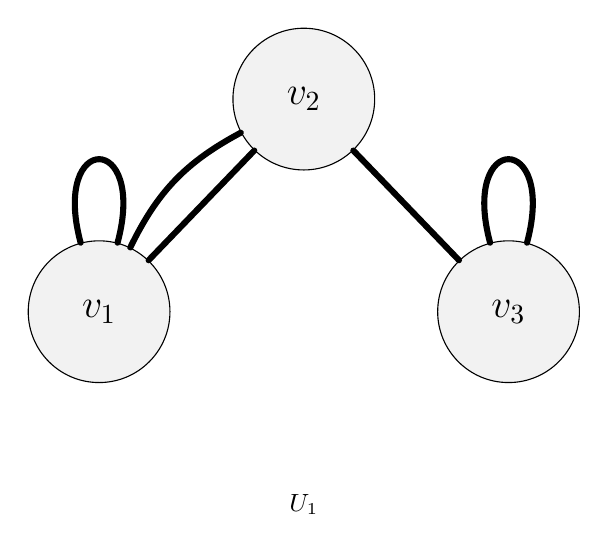
\begin{tikzpicture}[
  ugv/.style={circle, draw=black, fill=gray!10, minimum size=18.0mm, inner sep=2.0pt, font={\Large}},
  ugedge/.style={line width=2.20pt, line cap=round}
]
\node[ugv] (u0) at (-2.60,0.00) {$v_{1}$};
\node[ugv] (u1) at (0.00,2.70) {$v_{2}$};
\node[ugv] (u2) at (2.60,0.00) {$v_{3}$};
\draw[ugedge] (u0) to[loop above] (u0);
\draw[ugedge] (u0) -- (u1);
\draw[ugedge] (u0) to[bend left=18] (u1);
\draw[ugedge] (u1) -- (u2);
\draw[ugedge] (u2) to[loop above] (u2);
\node[font={\small}] at (0,-2.45) {$U_1$};
\end{tikzpicture}%
}
\end{center}
\item $U_2$.
\begin{center}
\resizebox{0.52\linewidth}{!}{%
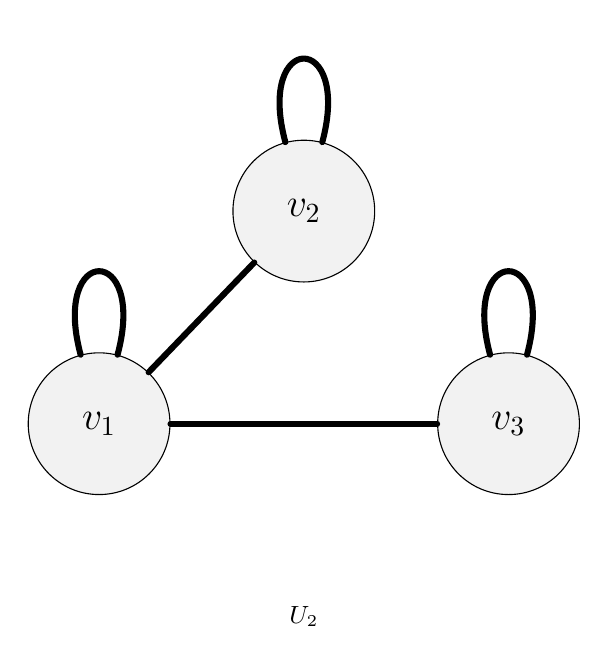
\begin{tikzpicture}[
  ugv/.style={circle, draw=black, fill=gray!10, minimum size=18.0mm, inner sep=2.0pt, font={\Large}},
  ugedge/.style={line width=2.20pt, line cap=round}
]
\node[ugv] (u0) at (-2.60,0.00) {$v_{1}$};
\node[ugv] (u1) at (0.00,2.70) {$v_{2}$};
\node[ugv] (u2) at (2.60,0.00) {$v_{3}$};
\draw[ugedge] (u0) to[loop above] (u0);
\draw[ugedge] (u0) -- (u1);
\draw[ugedge] (u0) -- (u2);
\draw[ugedge] (u1) to[loop above] (u1);
\draw[ugedge] (u2) to[loop above] (u2);
\node[font={\small}] at (0,-2.45) {$U_2$};
\end{tikzpicture}%
}
\end{center}
\item $U_3$.
\begin{center}
\resizebox{0.52\linewidth}{!}{%
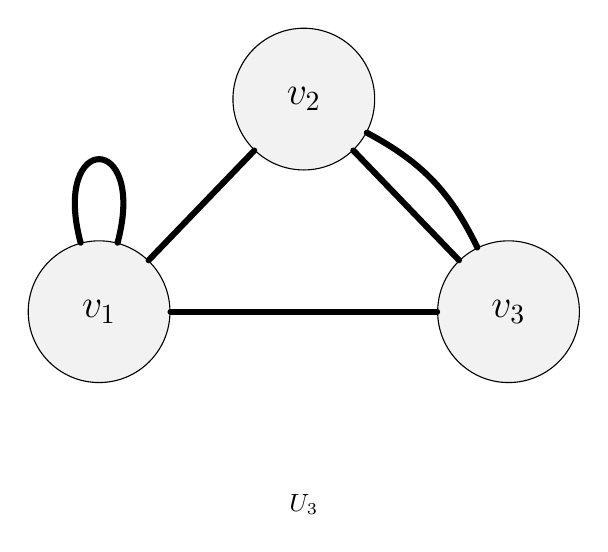
\begin{tikzpicture}[
  ugv/.style={circle, draw=black, fill=gray!10, minimum size=18.0mm, inner sep=2.0pt, font={\Large}},
  ugedge/.style={line width=2.20pt, line cap=round}
]
\node[ugv] (u0) at (-2.60,0.00) {$v_{1}$};
\node[ugv] (u1) at (0.00,2.70) {$v_{2}$};
\node[ugv] (u2) at (2.60,0.00) {$v_{3}$};
\draw[ugedge] (u0) to[loop above] (u0);
\draw[ugedge] (u0) -- (u1);
\draw[ugedge] (u0) -- (u2);
\draw[ugedge] (u1) -- (u2);
\draw[ugedge] (u1) to[bend left=18] (u2);
\node[font={\small}] at (0,-2.45) {$U_3$};
\end{tikzpicture}%
}
\end{center}
\item $U_4$.
\begin{center}
\resizebox{0.52\linewidth}{!}{%
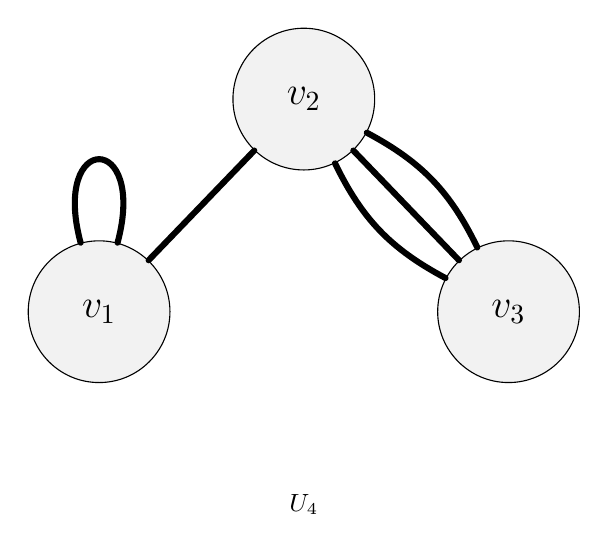
\begin{tikzpicture}[
  ugv/.style={circle, draw=black, fill=gray!10, minimum size=18.0mm, inner sep=2.0pt, font={\Large}},
  ugedge/.style={line width=2.20pt, line cap=round}
]
\node[ugv] (u0) at (-2.60,0.00) {$v_{1}$};
\node[ugv] (u1) at (0.00,2.70) {$v_{2}$};
\node[ugv] (u2) at (2.60,0.00) {$v_{3}$};
\draw[ugedge] (u0) to[loop above] (u0);
\draw[ugedge] (u0) -- (u1);
\draw[ugedge] (u1) -- (u2);
\draw[ugedge] (u1) to[bend left=18] (u2);
\draw[ugedge] (u1) to[bend right=18] (u2);
\node[font={\small}] at (0,-2.45) {$U_4$};
\end{tikzpicture}%
}
\end{center}
\item $U_5$.
\begin{center}
\resizebox{0.52\linewidth}{!}{%
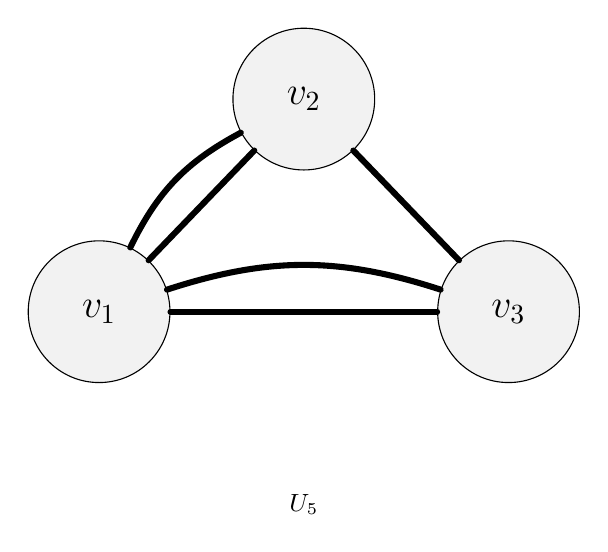
\begin{tikzpicture}[
  ugv/.style={circle, draw=black, fill=gray!10, minimum size=18.0mm, inner sep=2.0pt, font={\Large}},
  ugedge/.style={line width=2.20pt, line cap=round}
]
\node[ugv] (u0) at (-2.60,0.00) {$v_{1}$};
\node[ugv] (u1) at (0.00,2.70) {$v_{2}$};
\node[ugv] (u2) at (2.60,0.00) {$v_{3}$};
\draw[ugedge] (u0) -- (u1);
\draw[ugedge] (u0) to[bend left=18] (u1);
\draw[ugedge] (u0) -- (u2);
\draw[ugedge] (u0) to[bend left=18] (u2);
\draw[ugedge] (u1) -- (u2);
\node[font={\small}] at (0,-2.45) {$U_5$};
\end{tikzpicture}%
}
\end{center}
\end{enumerate}

\subsection*{Dictionary of graph labels used in preAUT/AUT}
For each graph label used above, this table records the corresponding ltt structure data.

\begin{enumerate}[leftmargin=*]
\item $G$:
\begin{itemize}[leftmargin=*]
\item underlying graph class $= U_5$.
\item red vertex $= x_{1}$.
\item red edge $= \{x_{1},\,\bar{x}_{5}\}$.
\item purple edges ($|\mathcal{P}|=9$):\mbox{}\\
$P_{1}: \{x_{2},\,x_{4}\},\; \{x_{2},\,x_{5}\},\; \{x_{4},\,x_{5}\}$\\
$P_{2}: \{x_{3},\,\bar{x}_{1}\},\; \{x_{3},\,\bar{x}_{2}\},\; \{\bar{x}_{1},\,\bar{x}_{2}\}$\\
$P_{3}: \{\bar{x}_{3},\,\bar{x}_{4}\},\; \{\bar{x}_{3},\,\bar{x}_{5}\},\; \{\bar{x}_{4},\,\bar{x}_{5}\}$.
\item black edges ($|\mathcal{B}|=5$): $\{x_{1},\,\bar{x}_{1}\},\; \{x_{2},\,\bar{x}_{2}\},\; \{x_{3},\,\bar{x}_{3}\},\; \{x_{4},\,\bar{x}_{4}\},\; \{x_{5},\,\bar{x}_{5}\}$.
\end{itemize}
\item $G_{1}$:
\begin{itemize}[leftmargin=*]
\item underlying graph class $= U_3$.
\item red vertex $= x_{1}$.
\item red edge $= \{x_{1},\,x_{3}\}$.
\item purple edges ($|\mathcal{P}|=9$):\mbox{}\\
$P_{1}: \{x_{2},\,x_{4}\},\; \{x_{2},\,x_{5}\},\; \{x_{4},\,x_{5}\}$\\
$P_{2}: \{x_{3},\,\bar{x}_{1}\},\; \{x_{3},\,\bar{x}_{2}\},\; \{\bar{x}_{1},\,\bar{x}_{2}\}$\\
$P_{3}: \{\bar{x}_{3},\,\bar{x}_{4}\},\; \{\bar{x}_{3},\,\bar{x}_{5}\},\; \{\bar{x}_{4},\,\bar{x}_{5}\}$.
\item black edges ($|\mathcal{B}|=5$): $\{x_{1},\,\bar{x}_{1}\},\; \{x_{2},\,\bar{x}_{2}\},\; \{x_{3},\,\bar{x}_{3}\},\; \{x_{4},\,\bar{x}_{4}\},\; \{x_{5},\,\bar{x}_{5}\}$.
\end{itemize}
\item $G_{2}$:
\begin{itemize}[leftmargin=*]
\item underlying graph class $= U_5$.
\item red vertex $= x_{1}$.
\item red edge $= \{x_{1},\,x_{4}\}$.
\item purple edges ($|\mathcal{P}|=9$):\mbox{}\\
$P_{1}: \{x_{2},\,x_{4}\},\; \{x_{2},\,x_{5}\},\; \{x_{4},\,x_{5}\}$\\
$P_{2}: \{x_{3},\,\bar{x}_{1}\},\; \{x_{3},\,\bar{x}_{2}\},\; \{\bar{x}_{1},\,\bar{x}_{2}\}$\\
$P_{3}: \{\bar{x}_{3},\,\bar{x}_{4}\},\; \{\bar{x}_{3},\,\bar{x}_{5}\},\; \{\bar{x}_{4},\,\bar{x}_{5}\}$.
\item black edges ($|\mathcal{B}|=5$): $\{x_{1},\,\bar{x}_{1}\},\; \{x_{2},\,\bar{x}_{2}\},\; \{x_{3},\,\bar{x}_{3}\},\; \{x_{4},\,\bar{x}_{4}\},\; \{x_{5},\,\bar{x}_{5}\}$.
\end{itemize}
\item $G_{3}$:
\begin{itemize}[leftmargin=*]
\item underlying graph class $= U_3$.
\item red vertex $= \bar{x}_{3}$.
\item red edge $= \{\bar{x}_{1},\,\bar{x}_{3}\}$.
\item purple edges ($|\mathcal{P}|=9$):\mbox{}\\
$P_{1}: \{x_{1},\,\bar{x}_{4}\},\; \{x_{1},\,\bar{x}_{5}\},\; \{\bar{x}_{4},\,\bar{x}_{5}\}$\\
$P_{2}: \{x_{2},\,x_{4}\},\; \{x_{2},\,x_{5}\},\; \{x_{4},\,x_{5}\}$\\
$P_{3}: \{x_{3},\,\bar{x}_{1}\},\; \{x_{3},\,\bar{x}_{2}\},\; \{\bar{x}_{1},\,\bar{x}_{2}\}$.
\item black edges ($|\mathcal{B}|=5$): $\{x_{1},\,\bar{x}_{1}\},\; \{x_{2},\,\bar{x}_{2}\},\; \{x_{3},\,\bar{x}_{3}\},\; \{x_{4},\,\bar{x}_{4}\},\; \{x_{5},\,\bar{x}_{5}\}$.
\end{itemize}
\item $G_{4}$:
\begin{itemize}[leftmargin=*]
\item underlying graph class $= U_5$.
\item red vertex $= \bar{x}_{4}$.
\item red edge $= \{\bar{x}_{1},\,\bar{x}_{4}\}$.
\item purple edges ($|\mathcal{P}|=9$):\mbox{}\\
$P_{1}: \{x_{1},\,\bar{x}_{3}\},\; \{x_{1},\,\bar{x}_{5}\},\; \{\bar{x}_{3},\,\bar{x}_{5}\}$\\
$P_{2}: \{x_{2},\,x_{4}\},\; \{x_{2},\,x_{5}\},\; \{x_{4},\,x_{5}\}$\\
$P_{3}: \{x_{3},\,\bar{x}_{1}\},\; \{x_{3},\,\bar{x}_{2}\},\; \{\bar{x}_{1},\,\bar{x}_{2}\}$.
\item black edges ($|\mathcal{B}|=5$): $\{x_{1},\,\bar{x}_{1}\},\; \{x_{2},\,\bar{x}_{2}\},\; \{x_{3},\,\bar{x}_{3}\},\; \{x_{4},\,\bar{x}_{4}\},\; \{x_{5},\,\bar{x}_{5}\}$.
\end{itemize}
\item $G_{5}$:
\begin{itemize}[leftmargin=*]
\item underlying graph class $= U_5$.
\item red vertex $= x_{1}$.
\item red edge $= \{x_{1},\,x_{2}\}$.
\item purple edges ($|\mathcal{P}|=9$):\mbox{}\\
$P_{1}: \{x_{2},\,x_{4}\},\; \{x_{2},\,x_{5}\},\; \{x_{4},\,x_{5}\}$\\
$P_{2}: \{x_{3},\,\bar{x}_{1}\},\; \{x_{3},\,\bar{x}_{2}\},\; \{\bar{x}_{1},\,\bar{x}_{2}\}$\\
$P_{3}: \{\bar{x}_{3},\,\bar{x}_{4}\},\; \{\bar{x}_{3},\,\bar{x}_{5}\},\; \{\bar{x}_{4},\,\bar{x}_{5}\}$.
\item black edges ($|\mathcal{B}|=5$): $\{x_{1},\,\bar{x}_{1}\},\; \{x_{2},\,\bar{x}_{2}\},\; \{x_{3},\,\bar{x}_{3}\},\; \{x_{4},\,\bar{x}_{4}\},\; \{x_{5},\,\bar{x}_{5}\}$.
\end{itemize}
\item $G_{6}$:
\begin{itemize}[leftmargin=*]
\item underlying graph class $= U_3$.
\item red vertex $= \bar{x}_{2}$.
\item red edge $= \{\bar{x}_{1},\,\bar{x}_{2}\}$.
\item purple edges ($|\mathcal{P}|=9$):\mbox{}\\
$P_{1}: \{x_{1},\,x_{3}\},\; \{x_{1},\,\bar{x}_{1}\},\; \{x_{3},\,\bar{x}_{1}\}$\\
$P_{2}: \{x_{2},\,x_{4}\},\; \{x_{2},\,x_{5}\},\; \{x_{4},\,x_{5}\}$\\
$P_{3}: \{\bar{x}_{3},\,\bar{x}_{4}\},\; \{\bar{x}_{3},\,\bar{x}_{5}\},\; \{\bar{x}_{4},\,\bar{x}_{5}\}$.
\item black edges ($|\mathcal{B}|=5$): $\{x_{1},\,\bar{x}_{1}\},\; \{x_{2},\,\bar{x}_{2}\},\; \{x_{3},\,\bar{x}_{3}\},\; \{x_{4},\,\bar{x}_{4}\},\; \{x_{5},\,\bar{x}_{5}\}$.
\end{itemize}
\item $G_{7}$:
\begin{itemize}[leftmargin=*]
\item underlying graph class $= U_5$.
\item red vertex $= x_{1}$.
\item red edge $= \{x_{1},\,\bar{x}_{4}\}$.
\item purple edges ($|\mathcal{P}|=9$):\mbox{}\\
$P_{1}: \{x_{2},\,x_{4}\},\; \{x_{2},\,x_{5}\},\; \{x_{4},\,x_{5}\}$\\
$P_{2}: \{x_{3},\,\bar{x}_{1}\},\; \{x_{3},\,\bar{x}_{2}\},\; \{\bar{x}_{1},\,\bar{x}_{2}\}$\\
$P_{3}: \{\bar{x}_{3},\,\bar{x}_{4}\},\; \{\bar{x}_{3},\,\bar{x}_{5}\},\; \{\bar{x}_{4},\,\bar{x}_{5}\}$.
\item black edges ($|\mathcal{B}|=5$): $\{x_{1},\,\bar{x}_{1}\},\; \{x_{2},\,\bar{x}_{2}\},\; \{x_{3},\,\bar{x}_{3}\},\; \{x_{4},\,\bar{x}_{4}\},\; \{x_{5},\,\bar{x}_{5}\}$.
\end{itemize}
\item $G_{8}$:
\begin{itemize}[leftmargin=*]
\item underlying graph class $= U_5$.
\item red vertex $= x_{4}$.
\item red edge $= \{x_{4},\,\bar{x}_{1}\}$.
\item purple edges ($|\mathcal{P}|=9$):\mbox{}\\
$P_{1}: \{x_{1},\,x_{2}\},\; \{x_{1},\,x_{5}\},\; \{x_{2},\,x_{5}\}$\\
$P_{2}: \{x_{3},\,\bar{x}_{1}\},\; \{x_{3},\,\bar{x}_{2}\},\; \{\bar{x}_{1},\,\bar{x}_{2}\}$\\
$P_{3}: \{\bar{x}_{3},\,\bar{x}_{4}\},\; \{\bar{x}_{3},\,\bar{x}_{5}\},\; \{\bar{x}_{4},\,\bar{x}_{5}\}$.
\item black edges ($|\mathcal{B}|=5$): $\{x_{1},\,\bar{x}_{1}\},\; \{x_{2},\,\bar{x}_{2}\},\; \{x_{3},\,\bar{x}_{3}\},\; \{x_{4},\,\bar{x}_{4}\},\; \{x_{5},\,\bar{x}_{5}\}$.
\end{itemize}
\item $G_{9}$:
\begin{itemize}[leftmargin=*]
\item underlying graph class $= U_5$.
\item red vertex $= x_{5}$.
\item red edge $= \{x_{5},\,\bar{x}_{1}\}$.
\item purple edges ($|\mathcal{P}|=9$):\mbox{}\\
$P_{1}: \{x_{1},\,x_{2}\},\; \{x_{1},\,x_{4}\},\; \{x_{2},\,x_{4}\}$\\
$P_{2}: \{x_{3},\,\bar{x}_{1}\},\; \{x_{3},\,\bar{x}_{2}\},\; \{\bar{x}_{1},\,\bar{x}_{2}\}$\\
$P_{3}: \{\bar{x}_{3},\,\bar{x}_{4}\},\; \{\bar{x}_{3},\,\bar{x}_{5}\},\; \{\bar{x}_{4},\,\bar{x}_{5}\}$.
\item black edges ($|\mathcal{B}|=5$): $\{x_{1},\,\bar{x}_{1}\},\; \{x_{2},\,\bar{x}_{2}\},\; \{x_{3},\,\bar{x}_{3}\},\; \{x_{4},\,\bar{x}_{4}\},\; \{x_{5},\,\bar{x}_{5}\}$.
\end{itemize}
\item $G_{10}$:
\begin{itemize}[leftmargin=*]
\item underlying graph class $= U_4$.
\item red vertex $= x_{3}$.
\item red edge $= \{x_{2},\,x_{3}\}$.
\item purple edges ($|\mathcal{P}|=9$):\mbox{}\\
$P_{1}: \{x_{1},\,\bar{x}_{1}\},\; \{x_{1},\,\bar{x}_{2}\},\; \{\bar{x}_{1},\,\bar{x}_{2}\}$\\
$P_{2}: \{x_{2},\,x_{4}\},\; \{x_{2},\,x_{5}\},\; \{x_{4},\,x_{5}\}$\\
$P_{3}: \{\bar{x}_{3},\,\bar{x}_{4}\},\; \{\bar{x}_{3},\,\bar{x}_{5}\},\; \{\bar{x}_{4},\,\bar{x}_{5}\}$.
\item black edges ($|\mathcal{B}|=5$): $\{x_{1},\,\bar{x}_{1}\},\; \{x_{2},\,\bar{x}_{2}\},\; \{x_{3},\,\bar{x}_{3}\},\; \{x_{4},\,\bar{x}_{4}\},\; \{x_{5},\,\bar{x}_{5}\}$.
\end{itemize}
\item $G_{11}$:
\begin{itemize}[leftmargin=*]
\item underlying graph class $= U_4$.
\item red vertex $= \bar{x}_{2}$.
\item red edge $= \{\bar{x}_{2},\,\bar{x}_{3}\}$.
\item purple edges ($|\mathcal{P}|=9$):\mbox{}\\
$P_{1}: \{x_{1},\,x_{3}\},\; \{x_{1},\,\bar{x}_{1}\},\; \{x_{3},\,\bar{x}_{1}\}$\\
$P_{2}: \{x_{2},\,x_{4}\},\; \{x_{2},\,x_{5}\},\; \{x_{4},\,x_{5}\}$\\
$P_{3}: \{\bar{x}_{3},\,\bar{x}_{4}\},\; \{\bar{x}_{3},\,\bar{x}_{5}\},\; \{\bar{x}_{4},\,\bar{x}_{5}\}$.
\item black edges ($|\mathcal{B}|=5$): $\{x_{1},\,\bar{x}_{1}\},\; \{x_{2},\,\bar{x}_{2}\},\; \{x_{3},\,\bar{x}_{3}\},\; \{x_{4},\,\bar{x}_{4}\},\; \{x_{5},\,\bar{x}_{5}\}$.
\end{itemize}
\item $G_{12}$:
\begin{itemize}[leftmargin=*]
\item underlying graph class $= U_1$.
\item red vertex $= x_{3}$.
\item red edge $= \{x_{3},\,\bar{x}_{4}\}$.
\item purple edges ($|\mathcal{P}|=9$):\mbox{}\\
$P_{1}: \{x_{1},\,\bar{x}_{1}\},\; \{x_{1},\,\bar{x}_{2}\},\; \{\bar{x}_{1},\,\bar{x}_{2}\}$\\
$P_{2}: \{x_{2},\,x_{4}\},\; \{x_{2},\,x_{5}\},\; \{x_{4},\,x_{5}\}$\\
$P_{3}: \{\bar{x}_{3},\,\bar{x}_{4}\},\; \{\bar{x}_{3},\,\bar{x}_{5}\},\; \{\bar{x}_{4},\,\bar{x}_{5}\}$.
\item black edges ($|\mathcal{B}|=5$): $\{x_{1},\,\bar{x}_{1}\},\; \{x_{2},\,\bar{x}_{2}\},\; \{x_{3},\,\bar{x}_{3}\},\; \{x_{4},\,\bar{x}_{4}\},\; \{x_{5},\,\bar{x}_{5}\}$.
\end{itemize}
\item $G_{13}$:
\begin{itemize}[leftmargin=*]
\item underlying graph class $= U_1$.
\item red vertex $= x_{3}$.
\item red edge $= \{x_{3},\,\bar{x}_{5}\}$.
\item purple edges ($|\mathcal{P}|=9$):\mbox{}\\
$P_{1}: \{x_{1},\,\bar{x}_{1}\},\; \{x_{1},\,\bar{x}_{2}\},\; \{\bar{x}_{1},\,\bar{x}_{2}\}$\\
$P_{2}: \{x_{2},\,x_{4}\},\; \{x_{2},\,x_{5}\},\; \{x_{4},\,x_{5}\}$\\
$P_{3}: \{\bar{x}_{3},\,\bar{x}_{4}\},\; \{\bar{x}_{3},\,\bar{x}_{5}\},\; \{\bar{x}_{4},\,\bar{x}_{5}\}$.
\item black edges ($|\mathcal{B}|=5$): $\{x_{1},\,\bar{x}_{1}\},\; \{x_{2},\,\bar{x}_{2}\},\; \{x_{3},\,\bar{x}_{3}\},\; \{x_{4},\,\bar{x}_{4}\},\; \{x_{5},\,\bar{x}_{5}\}$.
\end{itemize}
\item $G_{14}$:
\begin{itemize}[leftmargin=*]
\item underlying graph class $= U_1$.
\item red vertex $= x_{4}$.
\item red edge $= \{x_{4},\,\bar{x}_{3}\}$.
\item purple edges ($|\mathcal{P}|=9$):\mbox{}\\
$P_{1}: \{x_{1},\,\bar{x}_{1}\},\; \{x_{1},\,\bar{x}_{2}\},\; \{\bar{x}_{1},\,\bar{x}_{2}\}$\\
$P_{2}: \{x_{2},\,x_{3}\},\; \{x_{2},\,x_{5}\},\; \{x_{3},\,x_{5}\}$\\
$P_{3}: \{\bar{x}_{3},\,\bar{x}_{4}\},\; \{\bar{x}_{3},\,\bar{x}_{5}\},\; \{\bar{x}_{4},\,\bar{x}_{5}\}$.
\item black edges ($|\mathcal{B}|=5$): $\{x_{1},\,\bar{x}_{1}\},\; \{x_{2},\,\bar{x}_{2}\},\; \{x_{3},\,\bar{x}_{3}\},\; \{x_{4},\,\bar{x}_{4}\},\; \{x_{5},\,\bar{x}_{5}\}$.
\end{itemize}
\item $G_{15}$:
\begin{itemize}[leftmargin=*]
\item underlying graph class $= U_1$.
\item red vertex $= x_{5}$.
\item red edge $= \{x_{5},\,\bar{x}_{3}\}$.
\item purple edges ($|\mathcal{P}|=9$):\mbox{}\\
$P_{1}: \{x_{1},\,\bar{x}_{1}\},\; \{x_{1},\,\bar{x}_{2}\},\; \{\bar{x}_{1},\,\bar{x}_{2}\}$\\
$P_{2}: \{x_{2},\,x_{3}\},\; \{x_{2},\,x_{4}\},\; \{x_{3},\,x_{4}\}$\\
$P_{3}: \{\bar{x}_{3},\,\bar{x}_{4}\},\; \{\bar{x}_{3},\,\bar{x}_{5}\},\; \{\bar{x}_{4},\,\bar{x}_{5}\}$.
\item black edges ($|\mathcal{B}|=5$): $\{x_{1},\,\bar{x}_{1}\},\; \{x_{2},\,\bar{x}_{2}\},\; \{x_{3},\,\bar{x}_{3}\},\; \{x_{4},\,\bar{x}_{4}\},\; \{x_{5},\,\bar{x}_{5}\}$.
\end{itemize}
\item $G_{16}$:
\begin{itemize}[leftmargin=*]
\item underlying graph class $= U_4$.
\item red vertex $= x_{3}$.
\item red edge $= \{x_{3},\,x_{5}\}$.
\item purple edges ($|\mathcal{P}|=9$):\mbox{}\\
$P_{1}: \{x_{1},\,\bar{x}_{1}\},\; \{x_{1},\,\bar{x}_{2}\},\; \{\bar{x}_{1},\,\bar{x}_{2}\}$\\
$P_{2}: \{x_{2},\,x_{4}\},\; \{x_{2},\,x_{5}\},\; \{x_{4},\,x_{5}\}$\\
$P_{3}: \{\bar{x}_{3},\,\bar{x}_{4}\},\; \{\bar{x}_{3},\,\bar{x}_{5}\},\; \{\bar{x}_{4},\,\bar{x}_{5}\}$.
\item black edges ($|\mathcal{B}|=5$): $\{x_{1},\,\bar{x}_{1}\},\; \{x_{2},\,\bar{x}_{2}\},\; \{x_{3},\,\bar{x}_{3}\},\; \{x_{4},\,\bar{x}_{4}\},\; \{x_{5},\,\bar{x}_{5}\}$.
\end{itemize}
\item $G_{17}$:
\begin{itemize}[leftmargin=*]
\item underlying graph class $= U_1$.
\item red vertex $= \bar{x}_{5}$.
\item red edge $= \{\bar{x}_{3},\,\bar{x}_{5}\}$.
\item purple edges ($|\mathcal{P}|=9$):\mbox{}\\
$P_{1}: \{x_{1},\,\bar{x}_{1}\},\; \{x_{1},\,\bar{x}_{2}\},\; \{\bar{x}_{1},\,\bar{x}_{2}\}$\\
$P_{2}: \{x_{2},\,x_{4}\},\; \{x_{2},\,x_{5}\},\; \{x_{4},\,x_{5}\}$\\
$P_{3}: \{x_{3},\,\bar{x}_{3}\},\; \{x_{3},\,\bar{x}_{4}\},\; \{\bar{x}_{3},\,\bar{x}_{4}\}$.
\item black edges ($|\mathcal{B}|=5$): $\{x_{1},\,\bar{x}_{1}\},\; \{x_{2},\,\bar{x}_{2}\},\; \{x_{3},\,\bar{x}_{3}\},\; \{x_{4},\,\bar{x}_{4}\},\; \{x_{5},\,\bar{x}_{5}\}$.
\end{itemize}
\item $G_{18}$:
\begin{itemize}[leftmargin=*]
\item underlying graph class $= U_4$.
\item red vertex $= x_{2}$.
\item red edge $= \{x_{2},\,\bar{x}_{3}\}$.
\item purple edges ($|\mathcal{P}|=9$):\mbox{}\\
$P_{1}: \{x_{1},\,\bar{x}_{1}\},\; \{x_{1},\,\bar{x}_{2}\},\; \{\bar{x}_{1},\,\bar{x}_{2}\}$\\
$P_{2}: \{x_{3},\,x_{4}\},\; \{x_{3},\,x_{5}\},\; \{x_{4},\,x_{5}\}$\\
$P_{3}: \{\bar{x}_{3},\,\bar{x}_{4}\},\; \{\bar{x}_{3},\,\bar{x}_{5}\},\; \{\bar{x}_{4},\,\bar{x}_{5}\}$.
\item black edges ($|\mathcal{B}|=5$): $\{x_{1},\,\bar{x}_{1}\},\; \{x_{2},\,\bar{x}_{2}\},\; \{x_{3},\,\bar{x}_{3}\},\; \{x_{4},\,\bar{x}_{4}\},\; \{x_{5},\,\bar{x}_{5}\}$.
\end{itemize}
\item $G_{19}$:
\begin{itemize}[leftmargin=*]
\item underlying graph class $= U_3$.
\item red vertex $= x_{3}$.
\item red edge $= \{x_{3},\,\bar{x}_{2}\}$.
\item purple edges ($|\mathcal{P}|=9$):\mbox{}\\
$P_{1}: \{x_{1},\,\bar{x}_{1}\},\; \{x_{1},\,\bar{x}_{2}\},\; \{\bar{x}_{1},\,\bar{x}_{2}\}$\\
$P_{2}: \{x_{2},\,x_{4}\},\; \{x_{2},\,x_{5}\},\; \{x_{4},\,x_{5}\}$\\
$P_{3}: \{\bar{x}_{3},\,\bar{x}_{4}\},\; \{\bar{x}_{3},\,\bar{x}_{5}\},\; \{\bar{x}_{4},\,\bar{x}_{5}\}$.
\item black edges ($|\mathcal{B}|=5$): $\{x_{1},\,\bar{x}_{1}\},\; \{x_{2},\,\bar{x}_{2}\},\; \{x_{3},\,\bar{x}_{3}\},\; \{x_{4},\,\bar{x}_{4}\},\; \{x_{5},\,\bar{x}_{5}\}$.
\end{itemize}
\item $G_{20}$:
\begin{itemize}[leftmargin=*]
\item underlying graph class $= U_2$.
\item red vertex $= \bar{x}_{4}$.
\item red edge $= \{x_{5},\,\bar{x}_{4}\}$.
\item purple edges ($|\mathcal{P}|=9$):\mbox{}\\
$P_{1}: \{x_{1},\,\bar{x}_{1}\},\; \{x_{1},\,\bar{x}_{2}\},\; \{\bar{x}_{1},\,\bar{x}_{2}\}$\\
$P_{2}: \{x_{2},\,x_{4}\},\; \{x_{2},\,x_{5}\},\; \{x_{4},\,x_{5}\}$\\
$P_{3}: \{x_{3},\,\bar{x}_{3}\},\; \{x_{3},\,\bar{x}_{5}\},\; \{\bar{x}_{3},\,\bar{x}_{5}\}$.
\item black edges ($|\mathcal{B}|=5$): $\{x_{1},\,\bar{x}_{1}\},\; \{x_{2},\,\bar{x}_{2}\},\; \{x_{3},\,\bar{x}_{3}\},\; \{x_{4},\,\bar{x}_{4}\},\; \{x_{5},\,\bar{x}_{5}\}$.
\end{itemize}
\item $G_{21}$:
\begin{itemize}[leftmargin=*]
\item underlying graph class $= U_2$.
\item red vertex $= \bar{x}_{5}$.
\item red edge $= \{x_{4},\,\bar{x}_{5}\}$.
\item purple edges ($|\mathcal{P}|=9$):\mbox{}\\
$P_{1}: \{x_{1},\,\bar{x}_{1}\},\; \{x_{1},\,\bar{x}_{2}\},\; \{\bar{x}_{1},\,\bar{x}_{2}\}$\\
$P_{2}: \{x_{2},\,x_{4}\},\; \{x_{2},\,x_{5}\},\; \{x_{4},\,x_{5}\}$\\
$P_{3}: \{x_{3},\,\bar{x}_{3}\},\; \{x_{3},\,\bar{x}_{4}\},\; \{\bar{x}_{3},\,\bar{x}_{4}\}$.
\item black edges ($|\mathcal{B}|=5$): $\{x_{1},\,\bar{x}_{1}\},\; \{x_{2},\,\bar{x}_{2}\},\; \{x_{3},\,\bar{x}_{3}\},\; \{x_{4},\,\bar{x}_{4}\},\; \{x_{5},\,\bar{x}_{5}\}$.
\end{itemize}
\item $G_{22}$:
\begin{itemize}[leftmargin=*]
\item underlying graph class $= U_4$.
\item red vertex $= x_{2}$.
\item red edge $= \{x_{2},\,x_{4}\}$.
\item purple edges ($|\mathcal{P}|=9$):\mbox{}\\
$P_{1}: \{x_{1},\,\bar{x}_{1}\},\; \{x_{1},\,\bar{x}_{2}\},\; \{\bar{x}_{1},\,\bar{x}_{2}\}$\\
$P_{2}: \{x_{3},\,x_{4}\},\; \{x_{3},\,x_{5}\},\; \{x_{4},\,x_{5}\}$\\
$P_{3}: \{\bar{x}_{3},\,\bar{x}_{4}\},\; \{\bar{x}_{3},\,\bar{x}_{5}\},\; \{\bar{x}_{4},\,\bar{x}_{5}\}$.
\item black edges ($|\mathcal{B}|=5$): $\{x_{1},\,\bar{x}_{1}\},\; \{x_{2},\,\bar{x}_{2}\},\; \{x_{3},\,\bar{x}_{3}\},\; \{x_{4},\,\bar{x}_{4}\},\; \{x_{5},\,\bar{x}_{5}\}$.
\end{itemize}
\item $G_{23}$:
\begin{itemize}[leftmargin=*]
\item underlying graph class $= U_4$.
\item red vertex $= x_{2}$.
\item red edge $= \{x_{2},\,x_{5}\}$.
\item purple edges ($|\mathcal{P}|=9$):\mbox{}\\
$P_{1}: \{x_{1},\,\bar{x}_{1}\},\; \{x_{1},\,\bar{x}_{2}\},\; \{\bar{x}_{1},\,\bar{x}_{2}\}$\\
$P_{2}: \{x_{3},\,x_{4}\},\; \{x_{3},\,x_{5}\},\; \{x_{4},\,x_{5}\}$\\
$P_{3}: \{\bar{x}_{3},\,\bar{x}_{4}\},\; \{\bar{x}_{3},\,\bar{x}_{5}\},\; \{\bar{x}_{4},\,\bar{x}_{5}\}$.
\item black edges ($|\mathcal{B}|=5$): $\{x_{1},\,\bar{x}_{1}\},\; \{x_{2},\,\bar{x}_{2}\},\; \{x_{3},\,\bar{x}_{3}\},\; \{x_{4},\,\bar{x}_{4}\},\; \{x_{5},\,\bar{x}_{5}\}$.
\end{itemize}
\item $G_{24}$:
\begin{itemize}[leftmargin=*]
\item underlying graph class $= U_3$.
\item red vertex $= \bar{x}_{4}$.
\item red edge $= \{\bar{x}_{2},\,\bar{x}_{4}\}$.
\item purple edges ($|\mathcal{P}|=9$):\mbox{}\\
$P_{1}: \{x_{1},\,\bar{x}_{1}\},\; \{x_{1},\,\bar{x}_{2}\},\; \{\bar{x}_{1},\,\bar{x}_{2}\}$\\
$P_{2}: \{x_{2},\,\bar{x}_{3}\},\; \{x_{2},\,\bar{x}_{5}\},\; \{\bar{x}_{3},\,\bar{x}_{5}\}$\\
$P_{3}: \{x_{3},\,x_{4}\},\; \{x_{3},\,x_{5}\},\; \{x_{4},\,x_{5}\}$.
\item black edges ($|\mathcal{B}|=5$): $\{x_{1},\,\bar{x}_{1}\},\; \{x_{2},\,\bar{x}_{2}\},\; \{x_{3},\,\bar{x}_{3}\},\; \{x_{4},\,\bar{x}_{4}\},\; \{x_{5},\,\bar{x}_{5}\}$.
\end{itemize}
\item $G_{25}$:
\begin{itemize}[leftmargin=*]
\item underlying graph class $= U_3$.
\item red vertex $= \bar{x}_{5}$.
\item red edge $= \{\bar{x}_{2},\,\bar{x}_{5}\}$.
\item purple edges ($|\mathcal{P}|=9$):\mbox{}\\
$P_{1}: \{x_{1},\,\bar{x}_{1}\},\; \{x_{1},\,\bar{x}_{2}\},\; \{\bar{x}_{1},\,\bar{x}_{2}\}$\\
$P_{2}: \{x_{2},\,\bar{x}_{3}\},\; \{x_{2},\,\bar{x}_{4}\},\; \{\bar{x}_{3},\,\bar{x}_{4}\}$\\
$P_{3}: \{x_{3},\,x_{4}\},\; \{x_{3},\,x_{5}\},\; \{x_{4},\,x_{5}\}$.
\item black edges ($|\mathcal{B}|=5$): $\{x_{1},\,\bar{x}_{1}\},\; \{x_{2},\,\bar{x}_{2}\},\; \{x_{3},\,\bar{x}_{3}\},\; \{x_{4},\,\bar{x}_{4}\},\; \{x_{5},\,\bar{x}_{5}\}$.
\end{itemize}
\item $G_{26}$:
\begin{itemize}[leftmargin=*]
\item underlying graph class $= U_5$.
\item red vertex $= x_{1}$.
\item red edge $= \{x_{1},\,\bar{x}_{3}\}$.
\item purple edges ($|\mathcal{P}|=9$):\mbox{}\\
$P_{1}: \{x_{2},\,x_{4}\},\; \{x_{2},\,x_{5}\},\; \{x_{4},\,x_{5}\}$\\
$P_{2}: \{x_{3},\,\bar{x}_{1}\},\; \{x_{3},\,\bar{x}_{2}\},\; \{\bar{x}_{1},\,\bar{x}_{2}\}$\\
$P_{3}: \{\bar{x}_{3},\,\bar{x}_{4}\},\; \{\bar{x}_{3},\,\bar{x}_{5}\},\; \{\bar{x}_{4},\,\bar{x}_{5}\}$.
\item black edges ($|\mathcal{B}|=5$): $\{x_{1},\,\bar{x}_{1}\},\; \{x_{2},\,\bar{x}_{2}\},\; \{x_{3},\,\bar{x}_{3}\},\; \{x_{4},\,\bar{x}_{4}\},\; \{x_{5},\,\bar{x}_{5}\}$.
\end{itemize}
\item $G_{27}$:
\begin{itemize}[leftmargin=*]
\item underlying graph class $= U_3$.
\item red vertex $= x_{3}$.
\item red edge $= \{x_{1},\,x_{3}\}$.
\item purple edges ($|\mathcal{P}|=9$):\mbox{}\\
$P_{1}: \{x_{1},\,\bar{x}_{1}\},\; \{x_{1},\,\bar{x}_{2}\},\; \{\bar{x}_{1},\,\bar{x}_{2}\}$\\
$P_{2}: \{x_{2},\,x_{4}\},\; \{x_{2},\,x_{5}\},\; \{x_{4},\,x_{5}\}$\\
$P_{3}: \{\bar{x}_{3},\,\bar{x}_{4}\},\; \{\bar{x}_{3},\,\bar{x}_{5}\},\; \{\bar{x}_{4},\,\bar{x}_{5}\}$.
\item black edges ($|\mathcal{B}|=5$): $\{x_{1},\,\bar{x}_{1}\},\; \{x_{2},\,\bar{x}_{2}\},\; \{x_{3},\,\bar{x}_{3}\},\; \{x_{4},\,\bar{x}_{4}\},\; \{x_{5},\,\bar{x}_{5}\}$.
\end{itemize}
\item $G_{28}$:
\begin{itemize}[leftmargin=*]
\item underlying graph class $= U_3$.
\item red vertex $= x_{3}$.
\item red edge $= \{x_{3},\,\bar{x}_{1}\}$.
\item purple edges ($|\mathcal{P}|=9$):\mbox{}\\
$P_{1}: \{x_{1},\,\bar{x}_{1}\},\; \{x_{1},\,\bar{x}_{2}\},\; \{\bar{x}_{1},\,\bar{x}_{2}\}$\\
$P_{2}: \{x_{2},\,x_{4}\},\; \{x_{2},\,x_{5}\},\; \{x_{4},\,x_{5}\}$\\
$P_{3}: \{\bar{x}_{3},\,\bar{x}_{4}\},\; \{\bar{x}_{3},\,\bar{x}_{5}\},\; \{\bar{x}_{4},\,\bar{x}_{5}\}$.
\item black edges ($|\mathcal{B}|=5$): $\{x_{1},\,\bar{x}_{1}\},\; \{x_{2},\,\bar{x}_{2}\},\; \{x_{3},\,\bar{x}_{3}\},\; \{x_{4},\,\bar{x}_{4}\},\; \{x_{5},\,\bar{x}_{5}\}$.
\end{itemize}
\item $G_{29}$:
\begin{itemize}[leftmargin=*]
\item underlying graph class $= U_5$.
\item red vertex $= \bar{x}_{1}$.
\item red edge $= \{\bar{x}_{1},\,\bar{x}_{3}\}$.
\item purple edges ($|\mathcal{P}|=9$):\mbox{}\\
$P_{1}: \{x_{1},\,x_{3}\},\; \{x_{1},\,\bar{x}_{2}\},\; \{x_{3},\,\bar{x}_{2}\}$\\
$P_{2}: \{x_{2},\,x_{4}\},\; \{x_{2},\,x_{5}\},\; \{x_{4},\,x_{5}\}$\\
$P_{3}: \{\bar{x}_{3},\,\bar{x}_{4}\},\; \{\bar{x}_{3},\,\bar{x}_{5}\},\; \{\bar{x}_{4},\,\bar{x}_{5}\}$.
\item black edges ($|\mathcal{B}|=5$): $\{x_{1},\,\bar{x}_{1}\},\; \{x_{2},\,\bar{x}_{2}\},\; \{x_{3},\,\bar{x}_{3}\},\; \{x_{4},\,\bar{x}_{4}\},\; \{x_{5},\,\bar{x}_{5}\}$.
\end{itemize}
\item $G_{30}$:
\begin{itemize}[leftmargin=*]
\item underlying graph class $= U_2$.
\item red vertex $= x_{2}$.
\item red edge $= \{x_{2},\,x_{4}\}$.
\item purple edges ($|\mathcal{P}|=9$):\mbox{}\\
$P_{1}: \{x_{1},\,\bar{x}_{1}\},\; \{x_{1},\,\bar{x}_{2}\},\; \{\bar{x}_{1},\,\bar{x}_{2}\}$\\
$P_{2}: \{x_{3},\,\bar{x}_{3}\},\; \{x_{3},\,\bar{x}_{5}\},\; \{\bar{x}_{3},\,\bar{x}_{5}\}$\\
$P_{3}: \{x_{4},\,x_{5}\},\; \{x_{4},\,\bar{x}_{4}\},\; \{x_{5},\,\bar{x}_{4}\}$.
\item black edges ($|\mathcal{B}|=5$): $\{x_{1},\,\bar{x}_{1}\},\; \{x_{2},\,\bar{x}_{2}\},\; \{x_{3},\,\bar{x}_{3}\},\; \{x_{4},\,\bar{x}_{4}\},\; \{x_{5},\,\bar{x}_{5}\}$.
\end{itemize}
\item $G_{31}$:
\begin{itemize}[leftmargin=*]
\item underlying graph class $= U_1$.
\item red vertex $= \bar{x}_{4}$.
\item red edge $= \{\bar{x}_{2},\,\bar{x}_{4}\}$.
\item purple edges ($|\mathcal{P}|=9$):\mbox{}\\
$P_{1}: \{x_{1},\,\bar{x}_{1}\},\; \{x_{1},\,\bar{x}_{2}\},\; \{\bar{x}_{1},\,\bar{x}_{2}\}$\\
$P_{2}: \{x_{2},\,x_{4}\},\; \{x_{2},\,x_{5}\},\; \{x_{4},\,x_{5}\}$\\
$P_{3}: \{x_{3},\,\bar{x}_{3}\},\; \{x_{3},\,\bar{x}_{5}\},\; \{\bar{x}_{3},\,\bar{x}_{5}\}$.
\item black edges ($|\mathcal{B}|=5$): $\{x_{1},\,\bar{x}_{1}\},\; \{x_{2},\,\bar{x}_{2}\},\; \{x_{3},\,\bar{x}_{3}\},\; \{x_{4},\,\bar{x}_{4}\},\; \{x_{5},\,\bar{x}_{5}\}$.
\end{itemize}
\item $G_{32}$:
\begin{itemize}[leftmargin=*]
\item underlying graph class $= U_2$.
\item red vertex $= x_{2}$.
\item red edge $= \{x_{2},\,\bar{x}_{5}\}$.
\item purple edges ($|\mathcal{P}|=9$):\mbox{}\\
$P_{1}: \{x_{1},\,\bar{x}_{1}\},\; \{x_{1},\,\bar{x}_{2}\},\; \{\bar{x}_{1},\,\bar{x}_{2}\}$\\
$P_{2}: \{x_{3},\,\bar{x}_{3}\},\; \{x_{3},\,\bar{x}_{5}\},\; \{\bar{x}_{3},\,\bar{x}_{5}\}$\\
$P_{3}: \{x_{4},\,x_{5}\},\; \{x_{4},\,\bar{x}_{4}\},\; \{x_{5},\,\bar{x}_{4}\}$.
\item black edges ($|\mathcal{B}|=5$): $\{x_{1},\,\bar{x}_{1}\},\; \{x_{2},\,\bar{x}_{2}\},\; \{x_{3},\,\bar{x}_{3}\},\; \{x_{4},\,\bar{x}_{4}\},\; \{x_{5},\,\bar{x}_{5}\}$.
\end{itemize}
\item $G_{33}$:
\begin{itemize}[leftmargin=*]
\item underlying graph class $= U_2$.
\item red vertex $= x_{5}$.
\item red edge $= \{x_{5},\,\bar{x}_{2}\}$.
\item purple edges ($|\mathcal{P}|=9$):\mbox{}\\
$P_{1}: \{x_{1},\,\bar{x}_{1}\},\; \{x_{1},\,\bar{x}_{2}\},\; \{\bar{x}_{1},\,\bar{x}_{2}\}$\\
$P_{2}: \{x_{2},\,x_{4}\},\; \{x_{2},\,\bar{x}_{4}\},\; \{x_{4},\,\bar{x}_{4}\}$\\
$P_{3}: \{x_{3},\,\bar{x}_{3}\},\; \{x_{3},\,\bar{x}_{5}\},\; \{\bar{x}_{3},\,\bar{x}_{5}\}$.
\item black edges ($|\mathcal{B}|=5$): $\{x_{1},\,\bar{x}_{1}\},\; \{x_{2},\,\bar{x}_{2}\},\; \{x_{3},\,\bar{x}_{3}\},\; \{x_{4},\,\bar{x}_{4}\},\; \{x_{5},\,\bar{x}_{5}\}$.
\end{itemize}
\item $G_{34}$:
\begin{itemize}[leftmargin=*]
\item underlying graph class $= U_4$.
\item red vertex $= x_{1}$.
\item red edge $= \{x_{1},\,x_{4}\}$.
\item purple edges ($|\mathcal{P}|=9$):\mbox{}\\
$P_{1}: \{x_{2},\,x_{4}\},\; \{x_{2},\,x_{5}\},\; \{x_{4},\,x_{5}\}$\\
$P_{2}: \{x_{3},\,\bar{x}_{3}\},\; \{x_{3},\,\bar{x}_{5}\},\; \{\bar{x}_{3},\,\bar{x}_{5}\}$\\
$P_{3}: \{\bar{x}_{1},\,\bar{x}_{2}\},\; \{\bar{x}_{1},\,\bar{x}_{4}\},\; \{\bar{x}_{2},\,\bar{x}_{4}\}$.
\item black edges ($|\mathcal{B}|=5$): $\{x_{1},\,\bar{x}_{1}\},\; \{x_{2},\,\bar{x}_{2}\},\; \{x_{3},\,\bar{x}_{3}\},\; \{x_{4},\,\bar{x}_{4}\},\; \{x_{5},\,\bar{x}_{5}\}$.
\end{itemize}
\item $G_{35}$:
\begin{itemize}[leftmargin=*]
\item underlying graph class $= U_4$.
\item red vertex $= \bar{x}_{1}$.
\item red edge $= \{x_{4},\,\bar{x}_{1}\}$.
\item purple edges ($|\mathcal{P}|=9$):\mbox{}\\
$P_{1}: \{x_{1},\,\bar{x}_{2}\},\; \{x_{1},\,\bar{x}_{4}\},\; \{\bar{x}_{2},\,\bar{x}_{4}\}$\\
$P_{2}: \{x_{2},\,x_{4}\},\; \{x_{2},\,x_{5}\},\; \{x_{4},\,x_{5}\}$\\
$P_{3}: \{x_{3},\,\bar{x}_{3}\},\; \{x_{3},\,\bar{x}_{5}\},\; \{\bar{x}_{3},\,\bar{x}_{5}\}$.
\item black edges ($|\mathcal{B}|=5$): $\{x_{1},\,\bar{x}_{1}\},\; \{x_{2},\,\bar{x}_{2}\},\; \{x_{3},\,\bar{x}_{3}\},\; \{x_{4},\,\bar{x}_{4}\},\; \{x_{5},\,\bar{x}_{5}\}$.
\end{itemize}
\item $G_{36}$:
\begin{itemize}[leftmargin=*]
\item underlying graph class $= U_1$.
\item red vertex $= \bar{x}_{4}$.
\item red edge $= \{x_{1},\,\bar{x}_{4}\}$.
\item purple edges ($|\mathcal{P}|=9$):\mbox{}\\
$P_{1}: \{x_{1},\,\bar{x}_{1}\},\; \{x_{1},\,\bar{x}_{2}\},\; \{\bar{x}_{1},\,\bar{x}_{2}\}$\\
$P_{2}: \{x_{2},\,x_{4}\},\; \{x_{2},\,x_{5}\},\; \{x_{4},\,x_{5}\}$\\
$P_{3}: \{x_{3},\,\bar{x}_{3}\},\; \{x_{3},\,\bar{x}_{5}\},\; \{\bar{x}_{3},\,\bar{x}_{5}\}$.
\item black edges ($|\mathcal{B}|=5$): $\{x_{1},\,\bar{x}_{1}\},\; \{x_{2},\,\bar{x}_{2}\},\; \{x_{3},\,\bar{x}_{3}\},\; \{x_{4},\,\bar{x}_{4}\},\; \{x_{5},\,\bar{x}_{5}\}$.
\end{itemize}
\item $G_{37}$:
\begin{itemize}[leftmargin=*]
\item underlying graph class $= U_1$.
\item red vertex $= \bar{x}_{4}$.
\item red edge $= \{\bar{x}_{1},\,\bar{x}_{4}\}$.
\item purple edges ($|\mathcal{P}|=9$):\mbox{}\\
$P_{1}: \{x_{1},\,\bar{x}_{1}\},\; \{x_{1},\,\bar{x}_{2}\},\; \{\bar{x}_{1},\,\bar{x}_{2}\}$\\
$P_{2}: \{x_{2},\,x_{4}\},\; \{x_{2},\,x_{5}\},\; \{x_{4},\,x_{5}\}$\\
$P_{3}: \{x_{3},\,\bar{x}_{3}\},\; \{x_{3},\,\bar{x}_{5}\},\; \{\bar{x}_{3},\,\bar{x}_{5}\}$.
\item black edges ($|\mathcal{B}|=5$): $\{x_{1},\,\bar{x}_{1}\},\; \{x_{2},\,\bar{x}_{2}\},\; \{x_{3},\,\bar{x}_{3}\},\; \{x_{4},\,\bar{x}_{4}\},\; \{x_{5},\,\bar{x}_{5}\}$.
\end{itemize}
\item $G_{38}$:
\begin{itemize}[leftmargin=*]
\item underlying graph class $= U_2$.
\item red vertex $= x_{2}$.
\item red edge $= \{x_{2},\,x_{3}\}$.
\item purple edges ($|\mathcal{P}|=9$):\mbox{}\\
$P_{1}: \{x_{1},\,\bar{x}_{1}\},\; \{x_{1},\,\bar{x}_{2}\},\; \{\bar{x}_{1},\,\bar{x}_{2}\}$\\
$P_{2}: \{x_{3},\,\bar{x}_{3}\},\; \{x_{3},\,\bar{x}_{5}\},\; \{\bar{x}_{3},\,\bar{x}_{5}\}$\\
$P_{3}: \{x_{4},\,x_{5}\},\; \{x_{4},\,\bar{x}_{4}\},\; \{x_{5},\,\bar{x}_{4}\}$.
\item black edges ($|\mathcal{B}|=5$): $\{x_{1},\,\bar{x}_{1}\},\; \{x_{2},\,\bar{x}_{2}\},\; \{x_{3},\,\bar{x}_{3}\},\; \{x_{4},\,\bar{x}_{4}\},\; \{x_{5},\,\bar{x}_{5}\}$.
\end{itemize}
\item $G_{39}$:
\begin{itemize}[leftmargin=*]
\item underlying graph class $= U_2$.
\item red vertex $= x_{2}$.
\item red edge $= \{x_{2},\,\bar{x}_{3}\}$.
\item purple edges ($|\mathcal{P}|=9$):\mbox{}\\
$P_{1}: \{x_{1},\,\bar{x}_{1}\},\; \{x_{1},\,\bar{x}_{2}\},\; \{\bar{x}_{1},\,\bar{x}_{2}\}$\\
$P_{2}: \{x_{3},\,\bar{x}_{3}\},\; \{x_{3},\,\bar{x}_{5}\},\; \{\bar{x}_{3},\,\bar{x}_{5}\}$\\
$P_{3}: \{x_{4},\,x_{5}\},\; \{x_{4},\,\bar{x}_{4}\},\; \{x_{5},\,\bar{x}_{4}\}$.
\item black edges ($|\mathcal{B}|=5$): $\{x_{1},\,\bar{x}_{1}\},\; \{x_{2},\,\bar{x}_{2}\},\; \{x_{3},\,\bar{x}_{3}\},\; \{x_{4},\,\bar{x}_{4}\},\; \{x_{5},\,\bar{x}_{5}\}$.
\end{itemize}
\item $G_{40}$:
\begin{itemize}[leftmargin=*]
\item underlying graph class $= U_1$.
\item red vertex $= x_{3}$.
\item red edge $= \{x_{3},\,\bar{x}_{2}\}$.
\item purple edges ($|\mathcal{P}|=9$):\mbox{}\\
$P_{1}: \{x_{1},\,\bar{x}_{1}\},\; \{x_{1},\,\bar{x}_{2}\},\; \{\bar{x}_{1},\,\bar{x}_{2}\}$\\
$P_{2}: \{x_{2},\,\bar{x}_{3}\},\; \{x_{2},\,\bar{x}_{5}\},\; \{\bar{x}_{3},\,\bar{x}_{5}\}$\\
$P_{3}: \{x_{4},\,x_{5}\},\; \{x_{4},\,\bar{x}_{4}\},\; \{x_{5},\,\bar{x}_{4}\}$.
\item black edges ($|\mathcal{B}|=5$): $\{x_{1},\,\bar{x}_{1}\},\; \{x_{2},\,\bar{x}_{2}\},\; \{x_{3},\,\bar{x}_{3}\},\; \{x_{4},\,\bar{x}_{4}\},\; \{x_{5},\,\bar{x}_{5}\}$.
\end{itemize}
\item $G_{41}$:
\begin{itemize}[leftmargin=*]
\item underlying graph class $= U_1$.
\item red vertex $= \bar{x}_{3}$.
\item red edge $= \{\bar{x}_{2},\,\bar{x}_{3}\}$.
\item purple edges ($|\mathcal{P}|=9$):\mbox{}\\
$P_{1}: \{x_{1},\,\bar{x}_{1}\},\; \{x_{1},\,\bar{x}_{2}\},\; \{\bar{x}_{1},\,\bar{x}_{2}\}$\\
$P_{2}: \{x_{2},\,x_{3}\},\; \{x_{2},\,\bar{x}_{5}\},\; \{x_{3},\,\bar{x}_{5}\}$\\
$P_{3}: \{x_{4},\,x_{5}\},\; \{x_{4},\,\bar{x}_{4}\},\; \{x_{5},\,\bar{x}_{4}\}$.
\item black edges ($|\mathcal{B}|=5$): $\{x_{1},\,\bar{x}_{1}\},\; \{x_{2},\,\bar{x}_{2}\},\; \{x_{3},\,\bar{x}_{3}\},\; \{x_{4},\,\bar{x}_{4}\},\; \{x_{5},\,\bar{x}_{5}\}$.
\end{itemize}
\end{enumerate}

\subsection*{Visual depiction of AUT by component (box-collapsed)}
AUT is computed from the box-collapsed preAUT (one node per box). Retained AUT components are listed sequentially. Nodes are labeled by Roman box IDs (I--XIV). Blue (Step~2) edge labels count only non-permutation arrows along that directed box pair; green labels count permutation ($\varphi$) edges, so blue and green labels sum to the total parallel preAUT arrows between those boxes.

\clearpage
\paragraph{AUT component $\mathrm{SCC}_{1}$.}
\vfill
\begin{center}
\setbox0=\hbox{%
\resizebox{!}{0.96\textheight}{%
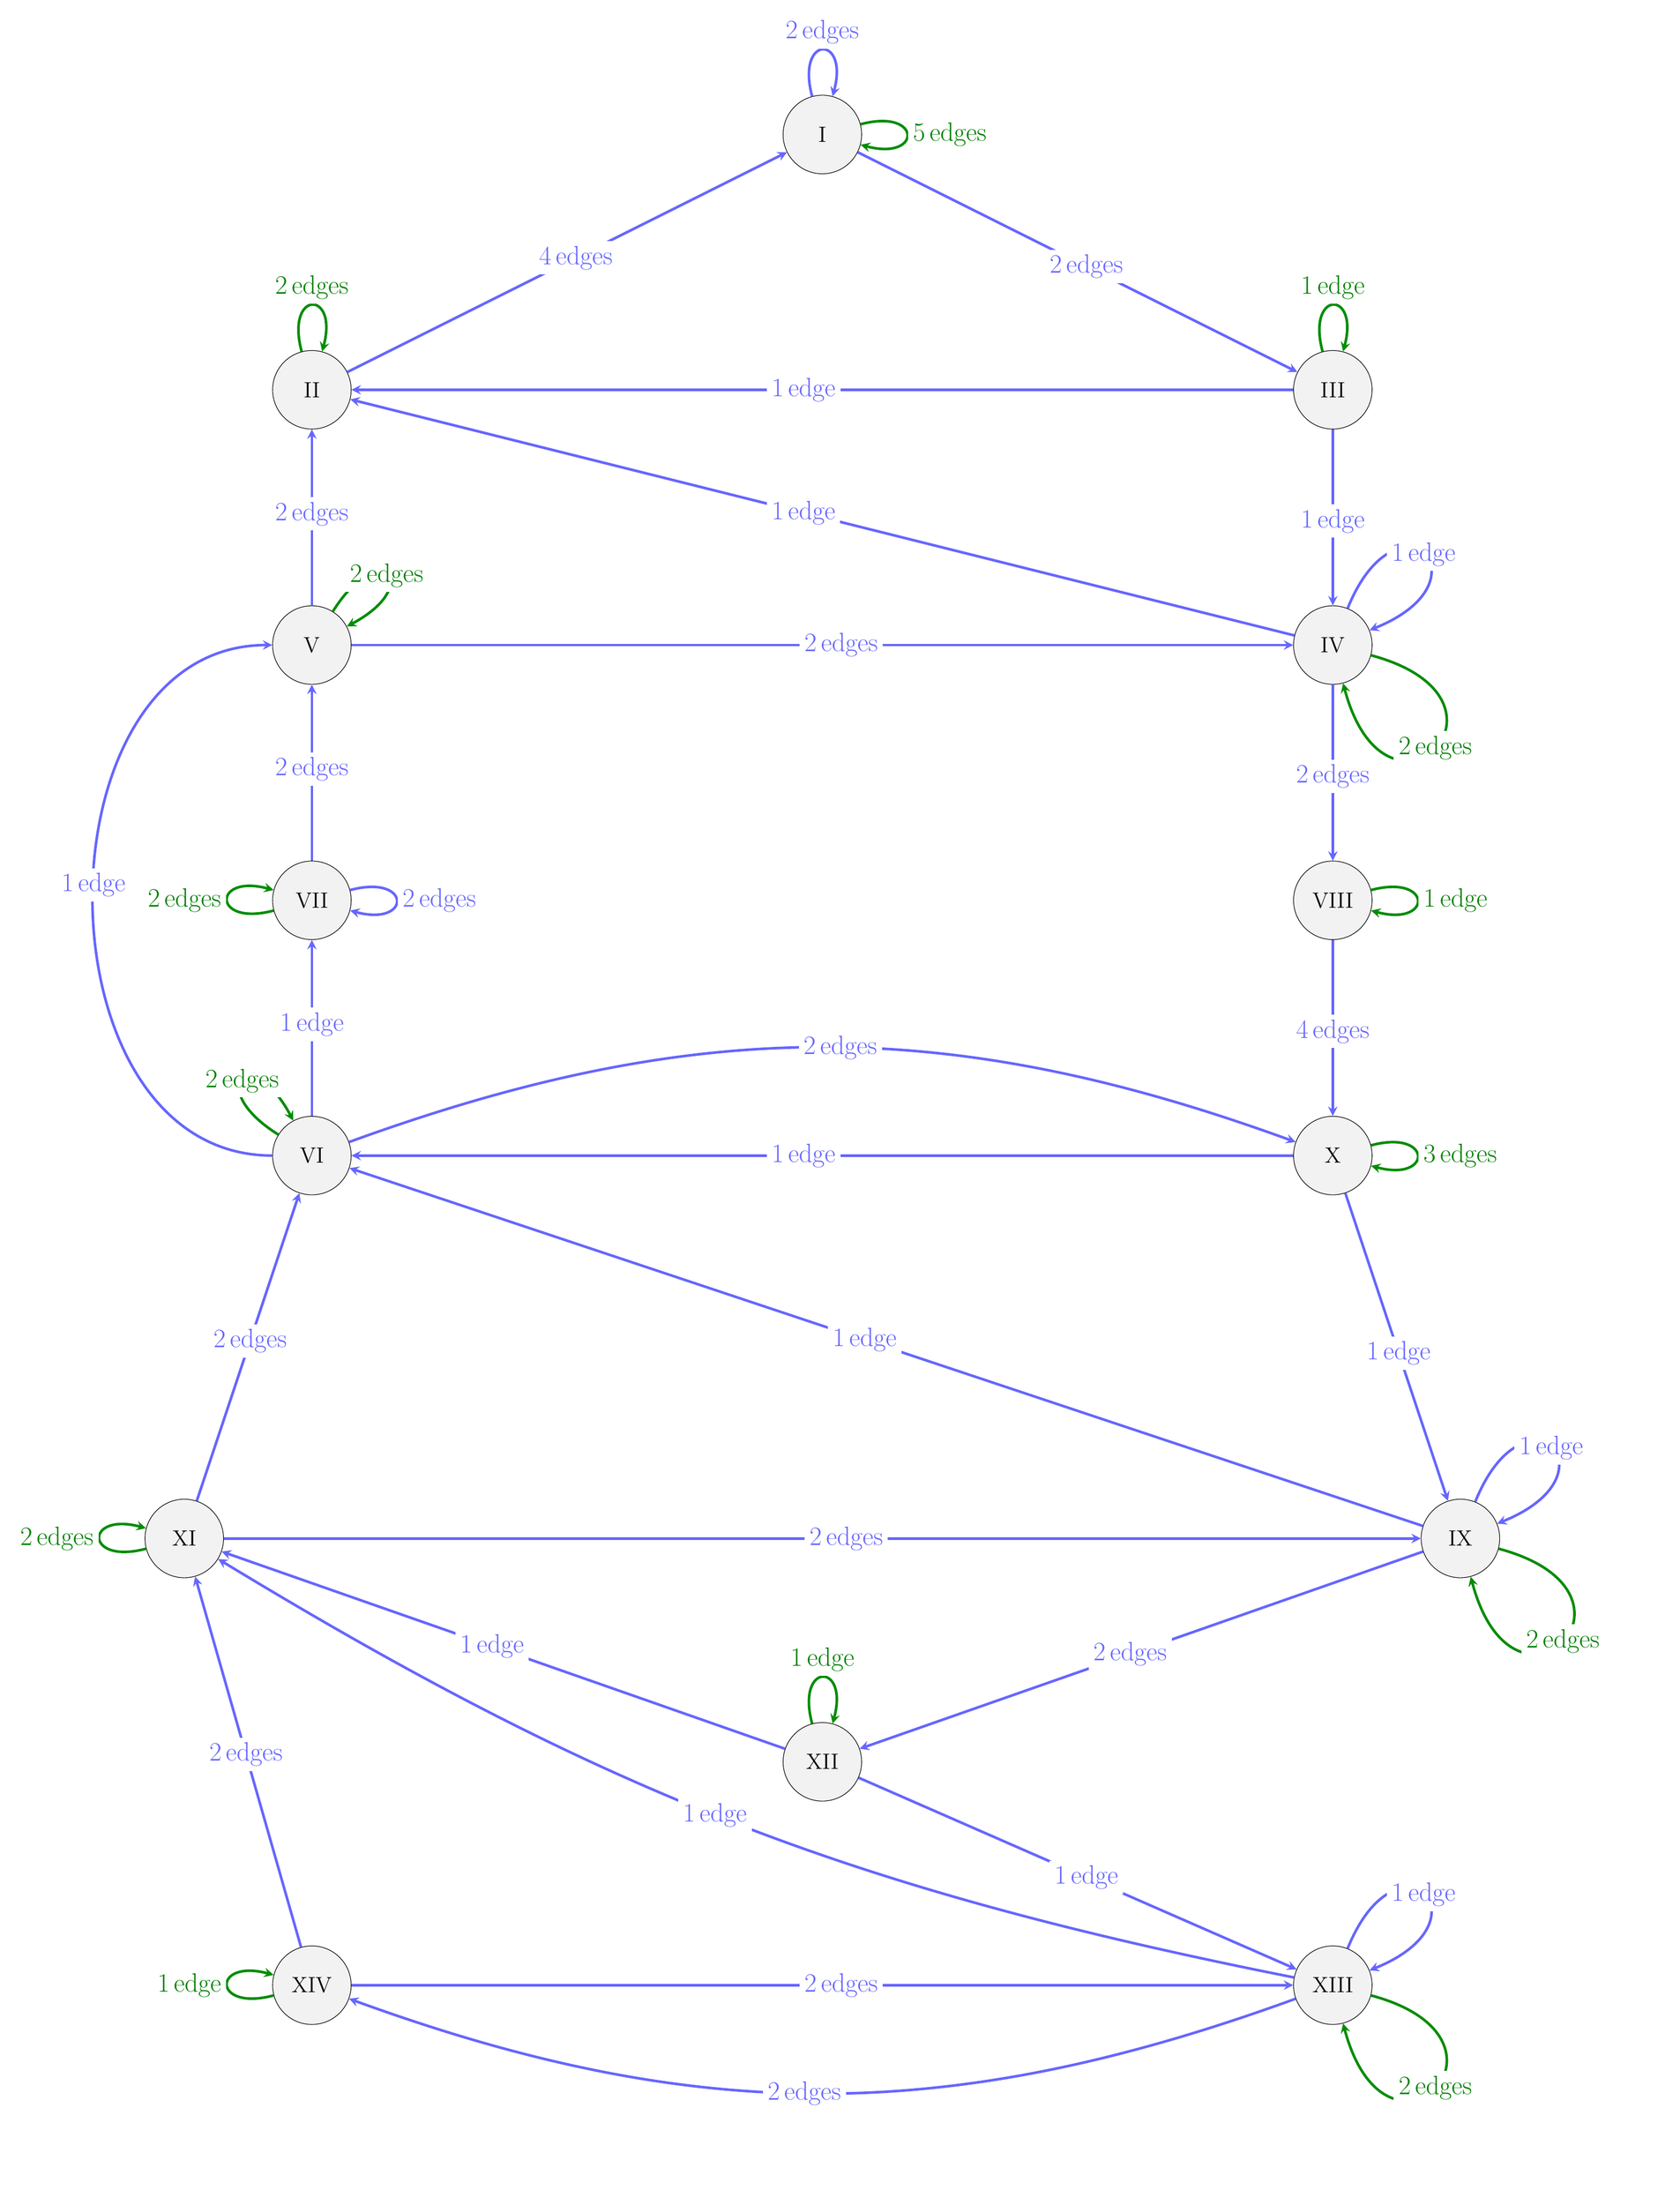
\begin{tikzpicture}[
  >=stealth,
  autnode/.style={circle, draw=black, fill=gray!10, minimum size=18.0mm, inner sep=2.8pt, font={\Large}},
  autedge/.style={->, draw=blue!60, line width=1.70pt},
  autlbl/.style={font={\LARGE}, transform shape, text=blue!60, fill=white, inner sep=3.2pt},
  autedgeperm/.style={->, draw=green!55!black, line width=1.70pt},
  autlblperm/.style={font={\LARGE}, transform shape, text=green!50!black, fill=white, inner sep=3.2pt}
]
\node[autnode] (n1) at (-11.7000,29.2500) {$\mathrm{II}$};
\node[autnode] (n2) at (0.0000,35.1000) {$\mathrm{I}$};
\node[autnode] (n3) at (-11.7000,17.5500) {$\mathrm{VII}$};
\node[autnode] (n4) at (11.7000,17.5500) {$\mathrm{VIII}$};
\node[autnode] (n5) at (-11.7000,11.7000) {$\mathrm{VI}$};
\node[autnode] (n6) at (11.7000,29.2500) {$\mathrm{III}$};
\node[autnode] (n7) at (11.7000,11.7000) {$\mathrm{X}$};
\node[autnode] (n8) at (0.0000,-2.1938) {$\mathrm{XII}$};
\node[autnode] (n9) at (11.7000,23.4000) {$\mathrm{IV}$};
\node[autnode] (n10) at (14.6250,2.9250) {$\mathrm{IX}$};
\node[autnode] (n11) at (11.7000,-7.3125) {$\mathrm{XIII}$};
\node[autnode] (n12) at (-11.7000,23.4000) {$\mathrm{V}$};
\node[autnode] (n13) at (-14.6250,2.9250) {$\mathrm{XI}$};
\node[autnode] (n14) at (-11.7000,-7.3125) {$\mathrm{XIV}$};
\draw[autedgeperm] (n1) to[loop above] node[autlblperm] {$ 2\,\mathrm{edges} $} (n1);
\draw[autedge] (n1) -- node[autlbl, pos=0.52] {$ 4\,\mathrm{edges} $} (n2);
\draw[autedge] (n2) to[loop above] node[autlbl] {$ 2\,\mathrm{edges} $} (n2);
\draw[autedgeperm] (n2) to[loop right] node[autlblperm] {$ 5\,\mathrm{edges} $} (n2);
\draw[autedge] (n2) -- node[autlbl, pos=0.52] {$ 2\,\mathrm{edges} $} (n6);
\draw[autedge] (n3) to[loop right] node[autlbl] {$ 2\,\mathrm{edges} $} (n3);
\draw[autedgeperm] (n3) to[loop left] node[autlblperm] {$ 2\,\mathrm{edges} $} (n3);
\draw[autedge] (n3) -- node[autlbl, pos=0.52] {$ 2\,\mathrm{edges} $} (n12);
\draw[autedgeperm] (n4) to[loop right] node[autlblperm] {$ 1\,\mathrm{edge} $} (n4);
\draw[autedge] (n4) -- node[autlbl, pos=0.52] {$ 4\,\mathrm{edges} $} (n7);
\draw[autedge] (n5) -- node[autlbl, pos=0.52] {$ 1\,\mathrm{edge} $} (n3);
\draw[autedgeperm] (n5) to[out=148,in=118,min distance=18mm,looseness=11] node[autlblperm] {$ 2\,\mathrm{edges} $} (n5);
\draw[autedge] (n5) to[bend left=20] node[autlbl, pos=0.52] {$ 2\,\mathrm{edges} $} (n7);
\draw[autedge] (n7) -- node[autlbl, pos=0.52] {$ 1\,\mathrm{edge} $} (n5);
\draw[autedge] (n5) to[out=180,in=180,looseness=1.2] node[autlbl, pos=0.52] {$ 1\,\mathrm{edge} $} (n12);
\draw[autedge] (n6) -- node[autlbl, pos=0.52] {$ 1\,\mathrm{edge} $} (n1);
\draw[autedgeperm] (n6) to[loop above] node[autlblperm] {$ 1\,\mathrm{edge} $} (n6);
\draw[autedge] (n6) -- node[autlbl, pos=0.52] {$ 1\,\mathrm{edge} $} (n9);
\draw[autedgeperm] (n7) to[loop right] node[autlblperm] {$ 3\,\mathrm{edges} $} (n7);
\draw[autedge] (n7) -- node[autlbl, pos=0.52] {$ 1\,\mathrm{edge} $} (n10);
\draw[autedgeperm] (n8) to[loop above] node[autlblperm] {$ 1\,\mathrm{edge} $} (n8);
\draw[autedge] (n8) -- node[autlbl, pos=0.52] {$ 1\,\mathrm{edge} $} (n11);
\draw[autedge] (n8) -- node[autlbl, pos=0.52] {$ 1\,\mathrm{edge} $} (n13);
\draw[autedge] (n9) -- node[autlbl, pos=0.52] {$ 1\,\mathrm{edge} $} (n1);
\draw[autedge] (n9) -- node[autlbl, pos=0.52] {$ 2\,\mathrm{edges} $} (n4);
\draw[autedge] (n9) to[out=68,in=22,min distance=18mm,looseness=11] node[autlbl] {$ 1\,\mathrm{edge} $} (n9);
\draw[autedgeperm] (n9) to[out=345,in=285,min distance=21.5mm,looseness=11] node[autlblperm] {$ 2\,\mathrm{edges} $} (n9);
\draw[autedge] (n10) -- node[autlbl, pos=0.52] {$ 1\,\mathrm{edge} $} (n5);
\draw[autedge] (n10) -- node[autlbl, pos=0.52] {$ 2\,\mathrm{edges} $} (n8);
\draw[autedge] (n10) to[out=68,in=22,min distance=18mm,looseness=11] node[autlbl] {$ 1\,\mathrm{edge} $} (n10);
\draw[autedgeperm] (n10) to[out=345,in=285,min distance=21.5mm,looseness=11] node[autlblperm] {$ 2\,\mathrm{edges} $} (n10);
\draw[autedge] (n11) to[out=68,in=22,min distance=18mm,looseness=11] node[autlbl] {$ 1\,\mathrm{edge} $} (n11);
\draw[autedgeperm] (n11) to[out=345,in=285,min distance=21.5mm,looseness=11] node[autlblperm] {$ 2\,\mathrm{edges} $} (n11);
\draw[autedge] (n11) to[bend left=10] node[autlbl, pos=0.52] {$ 1\,\mathrm{edge} $} (n13);
\draw[autedge] (n11) to[bend left=20] node[autlbl, pos=0.52] {$ 2\,\mathrm{edges} $} (n14);
\draw[autedge] (n14) -- node[autlbl, pos=0.52] {$ 2\,\mathrm{edges} $} (n11);
\draw[autedge] (n12) -- node[autlbl, pos=0.52] {$ 2\,\mathrm{edges} $} (n1);
\draw[autedge] (n12) -- node[autlbl, pos=0.52] {$ 2\,\mathrm{edges} $} (n9);
\draw[autedgeperm] (n12) to[out=58,in=28,min distance=18mm,looseness=11] node[autlblperm] {$ 2\,\mathrm{edges} $} (n12);
\draw[autedge] (n13) -- node[autlbl, pos=0.52] {$ 2\,\mathrm{edges} $} (n5);
\draw[autedge] (n13) -- node[autlbl, pos=0.52] {$ 2\,\mathrm{edges} $} (n10);
\draw[autedgeperm] (n13) to[loop left] node[autlblperm] {$ 2\,\mathrm{edges} $} (n13);
\draw[autedge] (n14) -- node[autlbl, pos=0.52] {$ 2\,\mathrm{edges} $} (n13);
\draw[autedgeperm] (n14) to[loop left] node[autlblperm] {$ 1\,\mathrm{edge} $} (n14);
\end{tikzpicture}%
}
}%
\ifdim\wd0>\dimexpr 1.0\linewidth\relax
  \resizebox{1.0\linewidth}{!}{\box0}%
\else
  \box0%
\fi
\end{center}

\vfill
\clearpage
\noindent\textit{Node index list for this component.}
\begin{itemize}[leftmargin=*]
\item Box $\mathrm{II}$ $= \mathrm{Class}_{1}\,(\mathrm{II})$.
\item Box $\mathrm{I}$ $= \mathrm{Class}_{2}\,(\mathrm{I})$.
\item Box $\mathrm{VII}$ $= \mathrm{Class}_{3}\,(\mathrm{VII})$.
\item Box $\mathrm{VIII}$ $= \mathrm{Class}_{4}\,(\mathrm{VIII})$.
\item Box $\mathrm{VI}$ $= \mathrm{Class}_{5}\,(\mathrm{VI})$.
\item Box $\mathrm{III}$ $= \mathrm{Class}_{6}\,(\mathrm{III})$.
\item Box $\mathrm{X}$ $= \mathrm{Class}_{7}\,(\mathrm{X})$.
\item Box $\mathrm{XII}$ $= \mathrm{Class}_{8}\,(\mathrm{XII})$.
\item Box $\mathrm{IV}$ $= \mathrm{Class}_{9}\,(\mathrm{IV})$.
\item Box $\mathrm{IX}$ $= \mathrm{Class}_{10}\,(\mathrm{IX})$.
\item Box $\mathrm{XIII}$ $= \mathrm{Class}_{11}\,(\mathrm{XIII})$.
\item Box $\mathrm{V}$ $= \mathrm{Class}_{12}\,(\mathrm{V})$.
\item Box $\mathrm{XI}$ $= \mathrm{Class}_{13}\,(\mathrm{XI})$.
\item Box $\mathrm{XIV}$ $= \mathrm{Class}_{14}\,(\mathrm{XIV})$.
\end{itemize}

\clearpage

\subsection*{Visual depiction of full preAUT (one node per box)}
This is the box-collapsed preAUT: each node is one Roman box (I--XIV). A directed edge is drawn from one box to another whenever preAUT has at least one edge between their corresponding classes. As in the AUT diagrams, blue counts Step~2 transitions only and green counts permutation ($\varphi$) edges along each directed box pair.

\paragraph{Box-collapsed preAUT component 1.}
\begin{center}
\resizebox{1.0000\linewidth}{!}{%
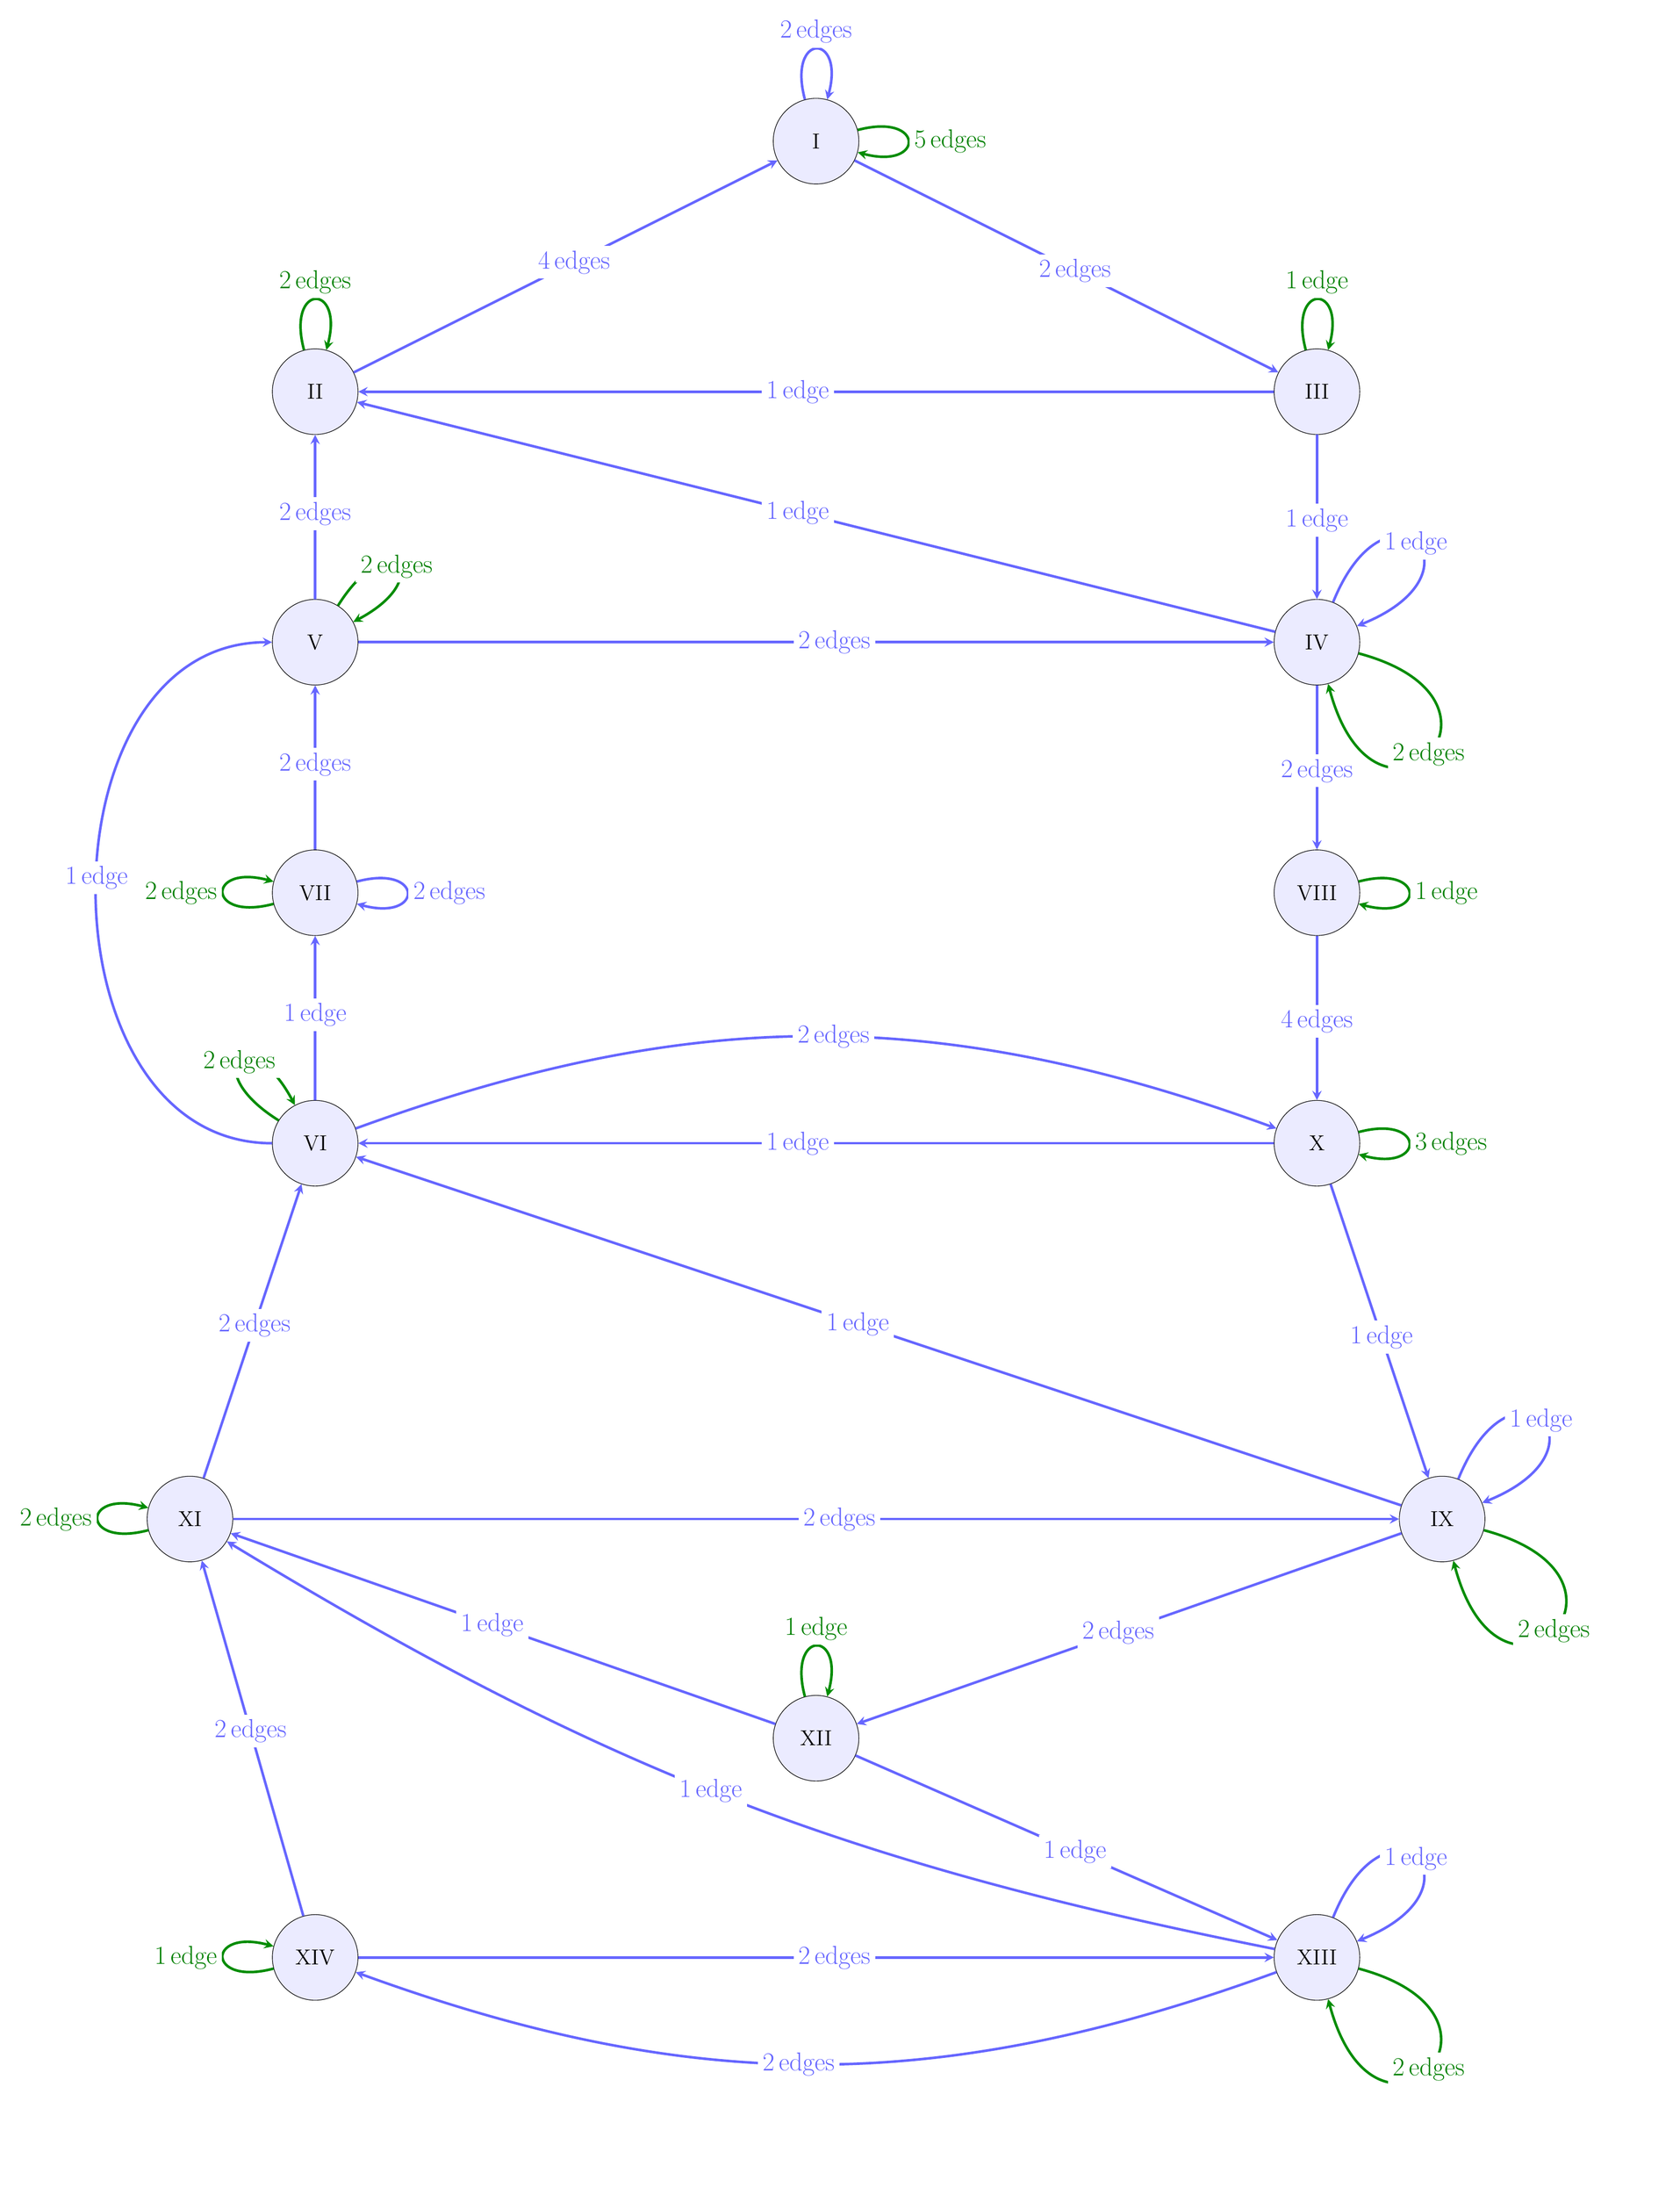
\begin{tikzpicture}[
  >=stealth,
  autnode/.style={circle, draw=black, fill=blue!8, minimum size=20.0mm, inner sep=3.2pt, font={\Large}},
  autedge/.style={->, draw=blue!60, line width=1.70pt},
  autlbl/.style={font={\LARGE}, transform shape, text=blue!60, fill=white, inner sep=3.2pt},
  autedgeperm/.style={->, draw=green!55!black, line width=1.70pt},
  autlblperm/.style={font={\LARGE}, transform shape, text=green!50!black, fill=white, inner sep=3.2pt}
]
\node[autnode] (n1) at (-11.7000,29.2500) {$\mathrm{II}$};
\node[autnode] (n2) at (0.0000,35.1000) {$\mathrm{I}$};
\node[autnode] (n3) at (-11.7000,17.5500) {$\mathrm{VII}$};
\node[autnode] (n4) at (11.7000,17.5500) {$\mathrm{VIII}$};
\node[autnode] (n5) at (-11.7000,11.7000) {$\mathrm{VI}$};
\node[autnode] (n6) at (11.7000,29.2500) {$\mathrm{III}$};
\node[autnode] (n7) at (11.7000,11.7000) {$\mathrm{X}$};
\node[autnode] (n8) at (0.0000,-2.1938) {$\mathrm{XII}$};
\node[autnode] (n9) at (11.7000,23.4000) {$\mathrm{IV}$};
\node[autnode] (n10) at (14.6250,2.9250) {$\mathrm{IX}$};
\node[autnode] (n11) at (11.7000,-7.3125) {$\mathrm{XIII}$};
\node[autnode] (n12) at (-11.7000,23.4000) {$\mathrm{V}$};
\node[autnode] (n13) at (-14.6250,2.9250) {$\mathrm{XI}$};
\node[autnode] (n14) at (-11.7000,-7.3125) {$\mathrm{XIV}$};
\draw[autedgeperm] (n1) to[loop above] node[autlblperm] {$ 2\,\mathrm{edges} $} (n1);
\draw[autedge] (n1) -- node[autlbl, pos=0.52] {$ 4\,\mathrm{edges} $} (n2);
\draw[autedge] (n2) to[loop above] node[autlbl] {$ 2\,\mathrm{edges} $} (n2);
\draw[autedgeperm] (n2) to[loop right] node[autlblperm] {$ 5\,\mathrm{edges} $} (n2);
\draw[autedge] (n2) -- node[autlbl, pos=0.52] {$ 2\,\mathrm{edges} $} (n6);
\draw[autedge] (n3) to[loop right] node[autlbl] {$ 2\,\mathrm{edges} $} (n3);
\draw[autedgeperm] (n3) to[loop left] node[autlblperm] {$ 2\,\mathrm{edges} $} (n3);
\draw[autedge] (n3) -- node[autlbl, pos=0.52] {$ 2\,\mathrm{edges} $} (n12);
\draw[autedgeperm] (n4) to[loop right] node[autlblperm] {$ 1\,\mathrm{edge} $} (n4);
\draw[autedge] (n4) -- node[autlbl, pos=0.52] {$ 4\,\mathrm{edges} $} (n7);
\draw[autedge] (n5) -- node[autlbl, pos=0.52] {$ 1\,\mathrm{edge} $} (n3);
\draw[autedgeperm] (n5) to[out=148,in=118,min distance=18mm,looseness=11] node[autlblperm] {$ 2\,\mathrm{edges} $} (n5);
\draw[autedge] (n5) to[bend left=20] node[autlbl, pos=0.52] {$ 2\,\mathrm{edges} $} (n7);
\draw[autedge] (n7) -- node[autlbl, pos=0.52] {$ 1\,\mathrm{edge} $} (n5);
\draw[autedge] (n5) to[out=180,in=180,looseness=1.2] node[autlbl, pos=0.52] {$ 1\,\mathrm{edge} $} (n12);
\draw[autedge] (n6) -- node[autlbl, pos=0.52] {$ 1\,\mathrm{edge} $} (n1);
\draw[autedgeperm] (n6) to[loop above] node[autlblperm] {$ 1\,\mathrm{edge} $} (n6);
\draw[autedge] (n6) -- node[autlbl, pos=0.52] {$ 1\,\mathrm{edge} $} (n9);
\draw[autedgeperm] (n7) to[loop right] node[autlblperm] {$ 3\,\mathrm{edges} $} (n7);
\draw[autedge] (n7) -- node[autlbl, pos=0.52] {$ 1\,\mathrm{edge} $} (n10);
\draw[autedgeperm] (n8) to[loop above] node[autlblperm] {$ 1\,\mathrm{edge} $} (n8);
\draw[autedge] (n8) -- node[autlbl, pos=0.52] {$ 1\,\mathrm{edge} $} (n11);
\draw[autedge] (n8) -- node[autlbl, pos=0.52] {$ 1\,\mathrm{edge} $} (n13);
\draw[autedge] (n9) -- node[autlbl, pos=0.52] {$ 1\,\mathrm{edge} $} (n1);
\draw[autedge] (n9) -- node[autlbl, pos=0.52] {$ 2\,\mathrm{edges} $} (n4);
\draw[autedge] (n9) to[out=68,in=22,min distance=18mm,looseness=11] node[autlbl] {$ 1\,\mathrm{edge} $} (n9);
\draw[autedgeperm] (n9) to[out=345,in=285,min distance=21.5mm,looseness=11] node[autlblperm] {$ 2\,\mathrm{edges} $} (n9);
\draw[autedge] (n10) -- node[autlbl, pos=0.52] {$ 1\,\mathrm{edge} $} (n5);
\draw[autedge] (n10) -- node[autlbl, pos=0.52] {$ 2\,\mathrm{edges} $} (n8);
\draw[autedge] (n10) to[out=68,in=22,min distance=18mm,looseness=11] node[autlbl] {$ 1\,\mathrm{edge} $} (n10);
\draw[autedgeperm] (n10) to[out=345,in=285,min distance=21.5mm,looseness=11] node[autlblperm] {$ 2\,\mathrm{edges} $} (n10);
\draw[autedge] (n11) to[out=68,in=22,min distance=18mm,looseness=11] node[autlbl] {$ 1\,\mathrm{edge} $} (n11);
\draw[autedgeperm] (n11) to[out=345,in=285,min distance=21.5mm,looseness=11] node[autlblperm] {$ 2\,\mathrm{edges} $} (n11);
\draw[autedge] (n11) to[bend left=10] node[autlbl, pos=0.52] {$ 1\,\mathrm{edge} $} (n13);
\draw[autedge] (n11) to[bend left=20] node[autlbl, pos=0.52] {$ 2\,\mathrm{edges} $} (n14);
\draw[autedge] (n14) -- node[autlbl, pos=0.52] {$ 2\,\mathrm{edges} $} (n11);
\draw[autedge] (n12) -- node[autlbl, pos=0.52] {$ 2\,\mathrm{edges} $} (n1);
\draw[autedge] (n12) -- node[autlbl, pos=0.52] {$ 2\,\mathrm{edges} $} (n9);
\draw[autedgeperm] (n12) to[out=58,in=28,min distance=18mm,looseness=11] node[autlblperm] {$ 2\,\mathrm{edges} $} (n12);
\draw[autedge] (n13) -- node[autlbl, pos=0.52] {$ 2\,\mathrm{edges} $} (n5);
\draw[autedge] (n13) -- node[autlbl, pos=0.52] {$ 2\,\mathrm{edges} $} (n10);
\draw[autedgeperm] (n13) to[loop left] node[autlblperm] {$ 2\,\mathrm{edges} $} (n13);
\draw[autedge] (n14) -- node[autlbl, pos=0.52] {$ 2\,\mathrm{edges} $} (n13);
\draw[autedgeperm] (n14) to[loop left] node[autlblperm] {$ 1\,\mathrm{edge} $} (n14);
\end{tikzpicture}%
}
\end{center}

\noindent\textit{Box index list for this preAUT diagram.}
\begin{itemize}[leftmargin=*]
\item Box $\mathrm{II}$ $= \mathrm{graphs}_{1}=\{G_{26}, G_{29}, G_{5}\}$.
\item Box $\mathrm{I}$ $= \mathrm{graphs}_{2}=\{G, G_{2}, G_{4}, G_{7}, G_{8}, G_{9}\}$.
\item Box $\mathrm{VII}$ $= \mathrm{graphs}_{3}=\{G_{18}, G_{22}, G_{23}\}$.
\item Box $\mathrm{VIII}$ $= \mathrm{graphs}_{4}=\{G_{10}, G_{11}\}$.
\item Box $\mathrm{VI}$ $= \mathrm{graphs}_{5}=\{G_{16}, G_{34}, G_{35}\}$.
\item Box $\mathrm{III}$ $= \mathrm{graphs}_{6}=\{G_{1}, G_{3}\}$.
\item Box $\mathrm{X}$ $= \mathrm{graphs}_{7}=\{G_{12}, G_{13}, G_{14}, G_{15}\}$.
\item Box $\mathrm{XII}$ $= \mathrm{graphs}_{8}=\{G_{20}, G_{21}\}$.
\item Box $\mathrm{IV}$ $= \mathrm{graphs}_{9}=\{G_{27}, G_{28}, G_{6}\}$.
\item Box $\mathrm{IX}$ $= \mathrm{graphs}_{10}=\{G_{17}, G_{36}, G_{37}\}$.
\item Box $\mathrm{XIII}$ $= \mathrm{graphs}_{11}=\{G_{30}, G_{38}, G_{39}\}$.
\item Box $\mathrm{V}$ $= \mathrm{graphs}_{12}=\{G_{19}, G_{24}, G_{25}\}$.
\item Box $\mathrm{XI}$ $= \mathrm{graphs}_{13}=\{G_{31}, G_{40}, G_{41}\}$.
\item Box $\mathrm{XIV}$ $= \mathrm{graphs}_{14}=\{G_{32}, G_{33}\}$.
\end{itemize}


\subsection*{preAUT edges omitted in AUT (cross-SCC/exiting edges)}
The AUT figures keep only edges whose source and target are in the same maximal SCC. The following preAUT edges leave those SCCs and are therefore omitted from AUT.

\begin{enumerate}[leftmargin=*]
\item From $\mathrm{SCC}_{1}$:
none.
\end{enumerate}

\subsection*{Visual depiction of omitted preAUT edges by SCC}
For each AUT component $\mathrm{SCC}_i$, we draw the edges that start in $\mathrm{SCC}_i$ and leave it in preAUT. Internal AUT edges are omitted in these diagrams.

\paragraph{Omitted preAUT edges from $\mathrm{SCC}_{1}$.}
\noindent None.


\subsection*{Step 6: coverage check across ep-isomorphism classes}
Covered ep-isomorphism classes: $14$ out of $14$. All classes are represented by the constructed preAUT, so no additional seed run is required.

\subsection*{Step 7: maximal SCCs and AUT (box-collapsed)}
Each maximal strongly connected component (SCC) of the box-collapsed preAUT is listed below; AUT is their disjoint union.

\paragraph{SCC decomposition of preAUT.}
\begin{enumerate}[leftmargin=*]
\item $\mathrm{SCC}_{1}=\{\mathrm{Class}_{1}\,(\mathrm{II}), \mathrm{Class}_{10}\,(\mathrm{IX}), \mathrm{Class}_{11}\,(\mathrm{XIII}), \mathrm{Class}_{12}\,(\mathrm{V}), \mathrm{Class}_{13}\,(\mathrm{XI}), \mathrm{Class}_{14}\,(\mathrm{XIV}), \mathrm{Class}_{2}\,(\mathrm{I}), \mathrm{Class}_{3}\,(\mathrm{VII}), \mathrm{Class}_{4}\,(\mathrm{VIII}), \mathrm{Class}_{5}\,(\mathrm{VI}), \mathrm{Class}_{6}\,(\mathrm{III}), \mathrm{Class}_{7}\,(\mathrm{X}), \mathrm{Class}_{8}\,(\mathrm{XII}), \mathrm{Class}_{9}\,(\mathrm{IV})\}$.
\end{enumerate}

\paragraph{Directed edges of AUT.}
These are exactly the box-collapsed preAUT edges whose endpoints lie in the same maximal SCC.
\begin{enumerate}[leftmargin=*]
\item $\mathrm{Class}_{1}\,(\mathrm{II}) \xrightarrow{2\,\mathrm{edges}} \mathrm{Class}_{1}\,(\mathrm{II})$ (inside $\mathrm{SCC}_{1}$).
\item $\mathrm{Class}_{1}\,(\mathrm{II}) \xrightarrow{4\,\mathrm{edges}} \mathrm{Class}_{2}\,(\mathrm{I})$ (inside $\mathrm{SCC}_{1}$).
\item $\mathrm{Class}_{2}\,(\mathrm{I}) \xrightarrow{7\,\mathrm{edges}} \mathrm{Class}_{2}\,(\mathrm{I})$ (inside $\mathrm{SCC}_{1}$).
\item $\mathrm{Class}_{2}\,(\mathrm{I}) \xrightarrow{2\,\mathrm{edges}} \mathrm{Class}_{6}\,(\mathrm{III})$ (inside $\mathrm{SCC}_{1}$).
\item $\mathrm{Class}_{3}\,(\mathrm{VII}) \xrightarrow{4\,\mathrm{edges}} \mathrm{Class}_{3}\,(\mathrm{VII})$ (inside $\mathrm{SCC}_{1}$).
\item $\mathrm{Class}_{3}\,(\mathrm{VII}) \xrightarrow{2\,\mathrm{edges}} \mathrm{Class}_{12}\,(\mathrm{V})$ (inside $\mathrm{SCC}_{1}$).
\item $\mathrm{Class}_{4}\,(\mathrm{VIII}) \xrightarrow{1\,\mathrm{edge}} \mathrm{Class}_{4}\,(\mathrm{VIII})$ (inside $\mathrm{SCC}_{1}$).
\item $\mathrm{Class}_{4}\,(\mathrm{VIII}) \xrightarrow{4\,\mathrm{edges}} \mathrm{Class}_{7}\,(\mathrm{X})$ (inside $\mathrm{SCC}_{1}$).
\item $\mathrm{Class}_{5}\,(\mathrm{VI}) \xrightarrow{1\,\mathrm{edge}} \mathrm{Class}_{3}\,(\mathrm{VII})$ (inside $\mathrm{SCC}_{1}$).
\item $\mathrm{Class}_{5}\,(\mathrm{VI}) \xrightarrow{2\,\mathrm{edges}} \mathrm{Class}_{5}\,(\mathrm{VI})$ (inside $\mathrm{SCC}_{1}$).
\item $\mathrm{Class}_{5}\,(\mathrm{VI}) \xrightarrow{2\,\mathrm{edges}} \mathrm{Class}_{7}\,(\mathrm{X})$ (inside $\mathrm{SCC}_{1}$).
\item $\mathrm{Class}_{5}\,(\mathrm{VI}) \xrightarrow{1\,\mathrm{edge}} \mathrm{Class}_{12}\,(\mathrm{V})$ (inside $\mathrm{SCC}_{1}$).
\item $\mathrm{Class}_{6}\,(\mathrm{III}) \xrightarrow{1\,\mathrm{edge}} \mathrm{Class}_{1}\,(\mathrm{II})$ (inside $\mathrm{SCC}_{1}$).
\item $\mathrm{Class}_{6}\,(\mathrm{III}) \xrightarrow{1\,\mathrm{edge}} \mathrm{Class}_{6}\,(\mathrm{III})$ (inside $\mathrm{SCC}_{1}$).
\item $\mathrm{Class}_{6}\,(\mathrm{III}) \xrightarrow{1\,\mathrm{edge}} \mathrm{Class}_{9}\,(\mathrm{IV})$ (inside $\mathrm{SCC}_{1}$).
\item $\mathrm{Class}_{7}\,(\mathrm{X}) \xrightarrow{1\,\mathrm{edge}} \mathrm{Class}_{5}\,(\mathrm{VI})$ (inside $\mathrm{SCC}_{1}$).
\item $\mathrm{Class}_{7}\,(\mathrm{X}) \xrightarrow{3\,\mathrm{edges}} \mathrm{Class}_{7}\,(\mathrm{X})$ (inside $\mathrm{SCC}_{1}$).
\item $\mathrm{Class}_{7}\,(\mathrm{X}) \xrightarrow{1\,\mathrm{edge}} \mathrm{Class}_{10}\,(\mathrm{IX})$ (inside $\mathrm{SCC}_{1}$).
\item $\mathrm{Class}_{8}\,(\mathrm{XII}) \xrightarrow{1\,\mathrm{edge}} \mathrm{Class}_{8}\,(\mathrm{XII})$ (inside $\mathrm{SCC}_{1}$).
\item $\mathrm{Class}_{8}\,(\mathrm{XII}) \xrightarrow{1\,\mathrm{edge}} \mathrm{Class}_{11}\,(\mathrm{XIII})$ (inside $\mathrm{SCC}_{1}$).
\item $\mathrm{Class}_{8}\,(\mathrm{XII}) \xrightarrow{1\,\mathrm{edge}} \mathrm{Class}_{13}\,(\mathrm{XI})$ (inside $\mathrm{SCC}_{1}$).
\item $\mathrm{Class}_{9}\,(\mathrm{IV}) \xrightarrow{1\,\mathrm{edge}} \mathrm{Class}_{1}\,(\mathrm{II})$ (inside $\mathrm{SCC}_{1}$).
\item $\mathrm{Class}_{9}\,(\mathrm{IV}) \xrightarrow{2\,\mathrm{edges}} \mathrm{Class}_{4}\,(\mathrm{VIII})$ (inside $\mathrm{SCC}_{1}$).
\item $\mathrm{Class}_{9}\,(\mathrm{IV}) \xrightarrow{3\,\mathrm{edges}} \mathrm{Class}_{9}\,(\mathrm{IV})$ (inside $\mathrm{SCC}_{1}$).
\item $\mathrm{Class}_{10}\,(\mathrm{IX}) \xrightarrow{1\,\mathrm{edge}} \mathrm{Class}_{5}\,(\mathrm{VI})$ (inside $\mathrm{SCC}_{1}$).
\item $\mathrm{Class}_{10}\,(\mathrm{IX}) \xrightarrow{2\,\mathrm{edges}} \mathrm{Class}_{8}\,(\mathrm{XII})$ (inside $\mathrm{SCC}_{1}$).
\item $\mathrm{Class}_{10}\,(\mathrm{IX}) \xrightarrow{3\,\mathrm{edges}} \mathrm{Class}_{10}\,(\mathrm{IX})$ (inside $\mathrm{SCC}_{1}$).
\item $\mathrm{Class}_{11}\,(\mathrm{XIII}) \xrightarrow{3\,\mathrm{edges}} \mathrm{Class}_{11}\,(\mathrm{XIII})$ (inside $\mathrm{SCC}_{1}$).
\item $\mathrm{Class}_{11}\,(\mathrm{XIII}) \xrightarrow{1\,\mathrm{edge}} \mathrm{Class}_{13}\,(\mathrm{XI})$ (inside $\mathrm{SCC}_{1}$).
\item $\mathrm{Class}_{11}\,(\mathrm{XIII}) \xrightarrow{2\,\mathrm{edges}} \mathrm{Class}_{14}\,(\mathrm{XIV})$ (inside $\mathrm{SCC}_{1}$).
\item $\mathrm{Class}_{12}\,(\mathrm{V}) \xrightarrow{2\,\mathrm{edges}} \mathrm{Class}_{1}\,(\mathrm{II})$ (inside $\mathrm{SCC}_{1}$).
\item $\mathrm{Class}_{12}\,(\mathrm{V}) \xrightarrow{2\,\mathrm{edges}} \mathrm{Class}_{9}\,(\mathrm{IV})$ (inside $\mathrm{SCC}_{1}$).
\item $\mathrm{Class}_{12}\,(\mathrm{V}) \xrightarrow{2\,\mathrm{edges}} \mathrm{Class}_{12}\,(\mathrm{V})$ (inside $\mathrm{SCC}_{1}$).
\item $\mathrm{Class}_{13}\,(\mathrm{XI}) \xrightarrow{2\,\mathrm{edges}} \mathrm{Class}_{5}\,(\mathrm{VI})$ (inside $\mathrm{SCC}_{1}$).
\item $\mathrm{Class}_{13}\,(\mathrm{XI}) \xrightarrow{2\,\mathrm{edges}} \mathrm{Class}_{10}\,(\mathrm{IX})$ (inside $\mathrm{SCC}_{1}$).
\item $\mathrm{Class}_{13}\,(\mathrm{XI}) \xrightarrow{2\,\mathrm{edges}} \mathrm{Class}_{13}\,(\mathrm{XI})$ (inside $\mathrm{SCC}_{1}$).
\item $\mathrm{Class}_{14}\,(\mathrm{XIV}) \xrightarrow{2\,\mathrm{edges}} \mathrm{Class}_{11}\,(\mathrm{XIII})$ (inside $\mathrm{SCC}_{1}$).
\item $\mathrm{Class}_{14}\,(\mathrm{XIV}) \xrightarrow{2\,\mathrm{edges}} \mathrm{Class}_{13}\,(\mathrm{XI})$ (inside $\mathrm{SCC}_{1}$).
\item $\mathrm{Class}_{14}\,(\mathrm{XIV}) \xrightarrow{1\,\mathrm{edge}} \mathrm{Class}_{14}\,(\mathrm{XIV})$ (inside $\mathrm{SCC}_{1}$).
\end{enumerate}


% Auto-generated by generate_box_internal_maps_appendix_tex.py — do not edit by hand.
\section[Box internal preAUT maps]{Internal preAUT maps within each ep-isomorphism class}

The Roman numeral for each class matches the translation table in the next section. Each diagram shows only edges whose source and target lie in the same class (edges induced inside one $\mathrm{graphs}_k$ box). \par\smallskip\noindent\textit{Regeneration.} Run \texttt{python generate\_box\_internal\_maps\_appendix\_tex.py} from the repository root.

\subsection*{Class $2$ (Box $\mathrm{I}$): internal preAUT maps}

\begin{center}
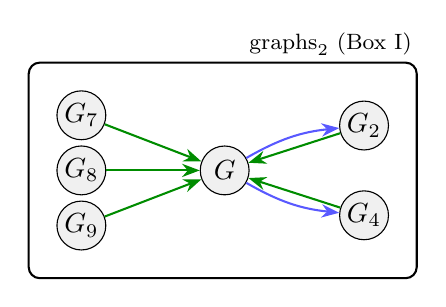
\begin{tikzpicture}[
  font=\normalsize,
  >=Stealth,
  grnode/.style={circle, draw=black, fill=gray!12, minimum size=6.2mm, inner sep=1pt},
  stepmap/.style={->, draw=blue!65, line width=0.75pt},
  permmap/.style={->, draw=green!55!black, line width=0.75pt}
]
  \node[grnode] (vG) at (0.00,0.00) {$G$};
  \node[grnode] (v2) at (1.77,0.57) {$G_{2}$};
  \node[grnode] (v4) at (1.77,-0.57) {$G_{4}$};
  \node[grnode] (v7) at (-1.82,0.70) {$G_{7}$};
  \node[grnode] (v8) at (-1.82,0.00) {$G_{8}$};
  \node[grnode] (v9) at (-1.82,-0.70) {$G_{9}$};
  \draw[stepmap] (vG) to[bend left=12] (v2);
  \draw[permmap] (v2) -- (vG);
  \draw[stepmap] (vG) to[bend right=12] (v4);
  \draw[permmap] (v4) -- (vG);
  \draw[permmap] (v7) -- (vG);
  \draw[permmap] (v8) -- (vG);
  \draw[permmap] (v9) -- (vG);
  \node[draw=black, line width=0.75pt, rounded corners=4pt, inner sep=10pt, fit=(vG)(v2)(v4)(v7)(v8)(v9)] (boxframe) {};
  \node[anchor=south east, inner sep=2pt, font=\footnotesize] at (boxframe.north east) {$\mathrm{graphs}_{2}$ (Box $\mathrm{I}$)};
\end{tikzpicture}
\end{center}
\begingroup\sloppy\normalsize\noindent
\raggedright
\textbf{Graph data (ltt structures in this box).}\par\smallskip\begin{enumerate}[leftmargin=*, itemsep=2pt]
\item $G$:
\begin{itemize}[leftmargin=*, itemsep=0pt]
\item underlying graph class $= U_5$.
\item red vertex $= x_{1}$.
\item red edge $= \{x_{1},\,\bar{x}_{5}\}$.
\item purple edges ($|\mathcal{P}|=9$):\mbox{}\\$P_{1}: \{x_{2},\,x_{4}\},\; \{x_{2},\,x_{5}\},\; \{x_{4},\,x_{5}\}$\\
$P_{2}: \{x_{3},\,\bar{x}_{1}\},\; \{x_{3},\,\bar{x}_{2}\},\; \{\bar{x}_{1},\,\bar{x}_{2}\}$\\
$P_{3}: \{\bar{x}_{3},\,\bar{x}_{4}\},\; \{\bar{x}_{3},\,\bar{x}_{5}\},\; \{\bar{x}_{4},\,\bar{x}_{5}\}$.
\item black edges ($|\mathcal{B}|=5$): $\{x_{1},\,\bar{x}_{1}\},\; \{x_{2},\,\bar{x}_{2}\},\; \{x_{3},\,\bar{x}_{3}\},\; \{x_{4},\,\bar{x}_{4}\},\; \{x_{5},\,\bar{x}_{5}\}$.
\end{itemize}
\item $G_{2}$:
\begin{itemize}[leftmargin=*, itemsep=0pt]
\item underlying graph class $= U_5$.
\item red vertex $= x_{1}$.
\item red edge $= \{x_{1},\,x_{4}\}$.
\item purple edges ($|\mathcal{P}|=9$):\mbox{}\\$P_{1}: \{x_{2},\,x_{4}\},\; \{x_{2},\,x_{5}\},\; \{x_{4},\,x_{5}\}$\\
$P_{2}: \{x_{3},\,\bar{x}_{1}\},\; \{x_{3},\,\bar{x}_{2}\},\; \{\bar{x}_{1},\,\bar{x}_{2}\}$\\
$P_{3}: \{\bar{x}_{3},\,\bar{x}_{4}\},\; \{\bar{x}_{3},\,\bar{x}_{5}\},\; \{\bar{x}_{4},\,\bar{x}_{5}\}$.
\item black edges ($|\mathcal{B}|=5$): $\{x_{1},\,\bar{x}_{1}\},\; \{x_{2},\,\bar{x}_{2}\},\; \{x_{3},\,\bar{x}_{3}\},\; \{x_{4},\,\bar{x}_{4}\},\; \{x_{5},\,\bar{x}_{5}\}$.
\end{itemize}
\item $G_{4}$:
\begin{itemize}[leftmargin=*, itemsep=0pt]
\item underlying graph class $= U_5$.
\item red vertex $= \bar{x}_{4}$.
\item red edge $= \{\bar{x}_{1},\,\bar{x}_{4}\}$.
\item purple edges ($|\mathcal{P}|=9$):\mbox{}\\$P_{1}: \{x_{1},\,\bar{x}_{3}\},\; \{x_{1},\,\bar{x}_{5}\},\; \{\bar{x}_{3},\,\bar{x}_{5}\}$\\
$P_{2}: \{x_{2},\,x_{4}\},\; \{x_{2},\,x_{5}\},\; \{x_{4},\,x_{5}\}$\\
$P_{3}: \{x_{3},\,\bar{x}_{1}\},\; \{x_{3},\,\bar{x}_{2}\},\; \{\bar{x}_{1},\,\bar{x}_{2}\}$.
\item black edges ($|\mathcal{B}|=5$): $\{x_{1},\,\bar{x}_{1}\},\; \{x_{2},\,\bar{x}_{2}\},\; \{x_{3},\,\bar{x}_{3}\},\; \{x_{4},\,\bar{x}_{4}\},\; \{x_{5},\,\bar{x}_{5}\}$.
\end{itemize}
\item $G_{7}$:
\begin{itemize}[leftmargin=*, itemsep=0pt]
\item underlying graph class $= U_5$.
\item red vertex $= x_{1}$.
\item red edge $= \{x_{1},\,\bar{x}_{4}\}$.
\item purple edges ($|\mathcal{P}|=9$):\mbox{}\\$P_{1}: \{x_{2},\,x_{4}\},\; \{x_{2},\,x_{5}\},\; \{x_{4},\,x_{5}\}$\\
$P_{2}: \{x_{3},\,\bar{x}_{1}\},\; \{x_{3},\,\bar{x}_{2}\},\; \{\bar{x}_{1},\,\bar{x}_{2}\}$\\
$P_{3}: \{\bar{x}_{3},\,\bar{x}_{4}\},\; \{\bar{x}_{3},\,\bar{x}_{5}\},\; \{\bar{x}_{4},\,\bar{x}_{5}\}$.
\item black edges ($|\mathcal{B}|=5$): $\{x_{1},\,\bar{x}_{1}\},\; \{x_{2},\,\bar{x}_{2}\},\; \{x_{3},\,\bar{x}_{3}\},\; \{x_{4},\,\bar{x}_{4}\},\; \{x_{5},\,\bar{x}_{5}\}$.
\end{itemize}
\item $G_{8}$:
\begin{itemize}[leftmargin=*, itemsep=0pt]
\item underlying graph class $= U_5$.
\item red vertex $= x_{4}$.
\item red edge $= \{x_{4},\,\bar{x}_{1}\}$.
\item purple edges ($|\mathcal{P}|=9$):\mbox{}\\$P_{1}: \{x_{1},\,x_{2}\},\; \{x_{1},\,x_{5}\},\; \{x_{2},\,x_{5}\}$\\
$P_{2}: \{x_{3},\,\bar{x}_{1}\},\; \{x_{3},\,\bar{x}_{2}\},\; \{\bar{x}_{1},\,\bar{x}_{2}\}$\\
$P_{3}: \{\bar{x}_{3},\,\bar{x}_{4}\},\; \{\bar{x}_{3},\,\bar{x}_{5}\},\; \{\bar{x}_{4},\,\bar{x}_{5}\}$.
\item black edges ($|\mathcal{B}|=5$): $\{x_{1},\,\bar{x}_{1}\},\; \{x_{2},\,\bar{x}_{2}\},\; \{x_{3},\,\bar{x}_{3}\},\; \{x_{4},\,\bar{x}_{4}\},\; \{x_{5},\,\bar{x}_{5}\}$.
\end{itemize}
\item $G_{9}$:
\begin{itemize}[leftmargin=*, itemsep=0pt]
\item underlying graph class $= U_5$.
\item red vertex $= x_{5}$.
\item red edge $= \{x_{5},\,\bar{x}_{1}\}$.
\item purple edges ($|\mathcal{P}|=9$):\mbox{}\\$P_{1}: \{x_{1},\,x_{2}\},\; \{x_{1},\,x_{4}\},\; \{x_{2},\,x_{4}\}$\\
$P_{2}: \{x_{3},\,\bar{x}_{1}\},\; \{x_{3},\,\bar{x}_{2}\},\; \{\bar{x}_{1},\,\bar{x}_{2}\}$\\
$P_{3}: \{\bar{x}_{3},\,\bar{x}_{4}\},\; \{\bar{x}_{3},\,\bar{x}_{5}\},\; \{\bar{x}_{4},\,\bar{x}_{5}\}$.
\item black edges ($|\mathcal{B}|=5$): $\{x_{1},\,\bar{x}_{1}\},\; \{x_{2},\,\bar{x}_{2}\},\; \{x_{3},\,\bar{x}_{3}\},\; \{x_{4},\,\bar{x}_{4}\},\; \{x_{5},\,\bar{x}_{5}\}$.
\end{itemize}
\end{enumerate}
\par\medskip
\textbf{Arrows.}\; Blue: Step~$2$ edge label. Green: permutation $\varphi$ from ep-isomorphism (Step~$3$). \par\smallskip\textbf{Maps represented (internal to Box~$\mathrm{I}$).}
\begin{enumerate}[leftmargin=*, itemsep=2pt]
\item $G \xrightarrow{x_{1} \to \bar{x}_{4}\,x_{1}} G_{2}$ \textit{(Step~2)}.
\item $G \xrightarrow{\bar{x}_{4} \to x_{1}\,\bar{x}_{4}} G_{4}$ \textit{(Step~2)}.
\item $G_{2} \xrightarrow{\varphi} G$, where $\varphi=x_{1} \mapsto x_{1},\; x_{2} \mapsto \bar{x}_{3},\; x_{3} \mapsto \bar{x}_{2},\; x_{4} \mapsto \bar{x}_{5},\; x_{5} \mapsto \bar{x}_{4}$ \textit{(permutation / ep-isomorphism).}
\item $G_{4} \xrightarrow{\varphi} G$, where $\varphi=x_{1} \mapsto x_{5},\; x_{2} \mapsto x_{3},\; x_{3} \mapsto \bar{x}_{4},\; x_{4} \mapsto \bar{x}_{1},\; x_{5} \mapsto \bar{x}_{2}$ \textit{(permutation / ep-isomorphism).}
\item $G_{7} \xrightarrow{\varphi} G$, where $\varphi=x_{1} \mapsto x_{1},\; x_{2} \mapsto x_{2},\; x_{3} \mapsto x_{3},\; x_{4} \mapsto x_{5},\; x_{5} \mapsto x_{4}$ \textit{(permutation / ep-isomorphism).}
\item $G_{8} \xrightarrow{\varphi} G$, where $\varphi=x_{1} \mapsto x_{5},\; x_{2} \mapsto x_{4},\; x_{3} \mapsto \bar{x}_{3},\; x_{4} \mapsto x_{1},\; x_{5} \mapsto x_{2}$ \textit{(permutation / ep-isomorphism).}
\item $G_{9} \xrightarrow{\varphi} G$, where $\varphi=x_{1} \mapsto x_{5},\; x_{2} \mapsto x_{4},\; x_{3} \mapsto \bar{x}_{3},\; x_{4} \mapsto x_{2},\; x_{5} \mapsto x_{1}$ \textit{(permutation / ep-isomorphism).}
\end{enumerate}
\par\medskip
\textbf{Incoming preAUT edges (into this box).}\par\smallskip
\begin{enumerate}[leftmargin=*, itemsep=2pt]
\item $G_{5} \xrightarrow{x_{1} \to x_{5}\,x_{1}} G$ {\footnotesize ($\mathrm{graphs}_{1}$, Box $\mathrm{II}$)} \textit{(Step~2)}.
\item $G_{5} \xrightarrow{x_{1} \to x_{4}\,x_{1}} G_{7}$ {\footnotesize ($\mathrm{graphs}_{1}$, Box $\mathrm{II}$)} \textit{(Step~2)}.
\item $G_{5} \xrightarrow{x_{4} \to x_{1}\,x_{4}} G_{8}$ {\footnotesize ($\mathrm{graphs}_{1}$, Box $\mathrm{II}$)} \textit{(Step~2)}.
\item $G_{5} \xrightarrow{x_{5} \to x_{1}\,x_{5}} G_{9}$ {\footnotesize ($\mathrm{graphs}_{1}$, Box $\mathrm{II}$)} \textit{(Step~2)}.
\end{enumerate}
\par\medskip
\textbf{Outgoing preAUT edges (from this box).}\par\smallskip
\begin{enumerate}[leftmargin=*, itemsep=2pt]
\item $G \xrightarrow{x_{1} \to \bar{x}_{3}\,x_{1}} G_{1}$ {\footnotesize ($\mathrm{graphs}_{6}$, Box $\mathrm{III}$)} \textit{(Step~2)}.
\item $G \xrightarrow{\bar{x}_{3} \to x_{1}\,\bar{x}_{3}} G_{3}$ {\footnotesize ($\mathrm{graphs}_{6}$, Box $\mathrm{III}$)} \textit{(Step~2)}.
\end{enumerate}
\par\endgroup

\subsection*{Class $1$ (Box $\mathrm{II}$): internal preAUT maps}

\begin{center}
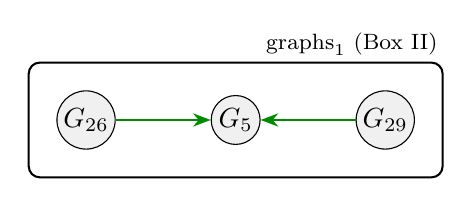
\begin{tikzpicture}[
  font=\normalsize,
  >=Stealth,
  grnode/.style={circle, draw=black, fill=gray!12, minimum size=6.2mm, inner sep=1pt},
  stepmap/.style={->, draw=blue!65, line width=0.75pt},
  permmap/.style={->, draw=green!55!black, line width=0.75pt}
]
  \node[grnode] (v5) at (0.00,0.00) {$G_{5}$};
  \node[grnode] (v26) at (-1.90,0.00) {$G_{26}$};
  \node[grnode] (v29) at (1.90,0.00) {$G_{29}$};
  \draw[permmap] (v26) -- (v5);
  \draw[permmap] (v29) -- (v5);
  \node[draw=black, line width=0.75pt, rounded corners=4pt, inner sep=10pt, fit=(v5)(v26)(v29)] (boxframe) {};
  \node[anchor=south east, inner sep=2pt, font=\footnotesize] at (boxframe.north east) {$\mathrm{graphs}_{1}$ (Box $\mathrm{II}$)};
\end{tikzpicture}
\end{center}
\begingroup\sloppy\normalsize\noindent
\raggedright
\textbf{Graph data (ltt structures in this box).}\par\smallskip\begin{enumerate}[leftmargin=*, itemsep=2pt]
\item $G_{5}$:
\begin{itemize}[leftmargin=*, itemsep=0pt]
\item underlying graph class $= U_5$.
\item red vertex $= x_{1}$.
\item red edge $= \{x_{1},\,x_{2}\}$.
\item purple edges ($|\mathcal{P}|=9$):\mbox{}\\$P_{1}: \{x_{2},\,x_{4}\},\; \{x_{2},\,x_{5}\},\; \{x_{4},\,x_{5}\}$\\
$P_{2}: \{x_{3},\,\bar{x}_{1}\},\; \{x_{3},\,\bar{x}_{2}\},\; \{\bar{x}_{1},\,\bar{x}_{2}\}$\\
$P_{3}: \{\bar{x}_{3},\,\bar{x}_{4}\},\; \{\bar{x}_{3},\,\bar{x}_{5}\},\; \{\bar{x}_{4},\,\bar{x}_{5}\}$.
\item black edges ($|\mathcal{B}|=5$): $\{x_{1},\,\bar{x}_{1}\},\; \{x_{2},\,\bar{x}_{2}\},\; \{x_{3},\,\bar{x}_{3}\},\; \{x_{4},\,\bar{x}_{4}\},\; \{x_{5},\,\bar{x}_{5}\}$.
\end{itemize}
\item $G_{26}$:
\begin{itemize}[leftmargin=*, itemsep=0pt]
\item underlying graph class $= U_5$.
\item red vertex $= x_{1}$.
\item red edge $= \{x_{1},\,\bar{x}_{3}\}$.
\item purple edges ($|\mathcal{P}|=9$):\mbox{}\\$P_{1}: \{x_{2},\,x_{4}\},\; \{x_{2},\,x_{5}\},\; \{x_{4},\,x_{5}\}$\\
$P_{2}: \{x_{3},\,\bar{x}_{1}\},\; \{x_{3},\,\bar{x}_{2}\},\; \{\bar{x}_{1},\,\bar{x}_{2}\}$\\
$P_{3}: \{\bar{x}_{3},\,\bar{x}_{4}\},\; \{\bar{x}_{3},\,\bar{x}_{5}\},\; \{\bar{x}_{4},\,\bar{x}_{5}\}$.
\item black edges ($|\mathcal{B}|=5$): $\{x_{1},\,\bar{x}_{1}\},\; \{x_{2},\,\bar{x}_{2}\},\; \{x_{3},\,\bar{x}_{3}\},\; \{x_{4},\,\bar{x}_{4}\},\; \{x_{5},\,\bar{x}_{5}\}$.
\end{itemize}
\item $G_{29}$:
\begin{itemize}[leftmargin=*, itemsep=0pt]
\item underlying graph class $= U_5$.
\item red vertex $= \bar{x}_{1}$.
\item red edge $= \{\bar{x}_{1},\,\bar{x}_{3}\}$.
\item purple edges ($|\mathcal{P}|=9$):\mbox{}\\$P_{1}: \{x_{1},\,x_{3}\},\; \{x_{1},\,\bar{x}_{2}\},\; \{x_{3},\,\bar{x}_{2}\}$\\
$P_{2}: \{x_{2},\,x_{4}\},\; \{x_{2},\,x_{5}\},\; \{x_{4},\,x_{5}\}$\\
$P_{3}: \{\bar{x}_{3},\,\bar{x}_{4}\},\; \{\bar{x}_{3},\,\bar{x}_{5}\},\; \{\bar{x}_{4},\,\bar{x}_{5}\}$.
\item black edges ($|\mathcal{B}|=5$): $\{x_{1},\,\bar{x}_{1}\},\; \{x_{2},\,\bar{x}_{2}\},\; \{x_{3},\,\bar{x}_{3}\},\; \{x_{4},\,\bar{x}_{4}\},\; \{x_{5},\,\bar{x}_{5}\}$.
\end{itemize}
\end{enumerate}
\par\medskip
\textbf{Arrows.}\; Blue: Step~$2$ edge label. Green: permutation $\varphi$ from ep-isomorphism (Step~$3$). \par\smallskip\textbf{Maps represented (internal to Box~$\mathrm{II}$).}
\begin{enumerate}[leftmargin=*, itemsep=2pt]
\item $G_{26} \xrightarrow{\varphi} G_{5}$, where $\varphi=x_{1} \mapsto x_{1},\; x_{2} \mapsto \bar{x}_{3},\; x_{3} \mapsto \bar{x}_{2},\; x_{4} \mapsto \bar{x}_{4},\; x_{5} \mapsto \bar{x}_{5}$ \textit{(permutation / ep-isomorphism).}
\item $G_{29} \xrightarrow{\varphi} G_{5}$, where $\varphi=x_{1} \mapsto \bar{x}_{1},\; x_{2} \mapsto \bar{x}_{3},\; x_{3} \mapsto \bar{x}_{2},\; x_{4} \mapsto \bar{x}_{4},\; x_{5} \mapsto \bar{x}_{5}$ \textit{(permutation / ep-isomorphism).}
\end{enumerate}
\par\medskip
\textbf{Incoming preAUT edges (into this box).}\par\smallskip
\begin{enumerate}[leftmargin=*, itemsep=2pt]
\item $G_{1} \xrightarrow{x_{1} \to \bar{x}_{2}\,x_{1}} G_{5}$ {\footnotesize ($\mathrm{graphs}_{6}$, Box $\mathrm{III}$)} \textit{(Step~2)}.
\item $G_{19} \xrightarrow{x_{1} \to x_{3}\,x_{1}} G_{26}$ {\footnotesize ($\mathrm{graphs}_{12}$, Box $\mathrm{V}$)} \textit{(Step~2)}.
\item $G_{19} \xrightarrow{\bar{x}_{1} \to x_{3}\,\bar{x}_{1}} G_{29}$ {\footnotesize ($\mathrm{graphs}_{12}$, Box $\mathrm{V}$)} \textit{(Step~2)}.
\item $G_{6} \xrightarrow{x_{1} \to \bar{x}_{2}\,x_{1}} G_{5}$ {\footnotesize ($\mathrm{graphs}_{9}$, Box $\mathrm{IV}$)} \textit{(Step~2)}.
\end{enumerate}
\par\medskip
\textbf{Outgoing preAUT edges (from this box).}\par\smallskip
\begin{enumerate}[leftmargin=*, itemsep=2pt]
\item $G_{5} \xrightarrow{x_{1} \to x_{5}\,x_{1}} G$ {\footnotesize ($\mathrm{graphs}_{2}$, Box $\mathrm{I}$)} \textit{(Step~2)}.
\item $G_{5} \xrightarrow{x_{1} \to x_{4}\,x_{1}} G_{7}$ {\footnotesize ($\mathrm{graphs}_{2}$, Box $\mathrm{I}$)} \textit{(Step~2)}.
\item $G_{5} \xrightarrow{x_{4} \to x_{1}\,x_{4}} G_{8}$ {\footnotesize ($\mathrm{graphs}_{2}$, Box $\mathrm{I}$)} \textit{(Step~2)}.
\item $G_{5} \xrightarrow{x_{5} \to x_{1}\,x_{5}} G_{9}$ {\footnotesize ($\mathrm{graphs}_{2}$, Box $\mathrm{I}$)} \textit{(Step~2)}.
\end{enumerate}
\par\endgroup

\subsection*{Class $6$ (Box $\mathrm{III}$): internal preAUT maps}

\begin{center}
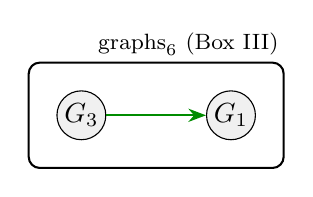
\begin{tikzpicture}[
  font=\normalsize,
  >=Stealth,
  grnode/.style={circle, draw=black, fill=gray!12, minimum size=6.2mm, inner sep=1pt},
  stepmap/.style={->, draw=blue!65, line width=0.75pt},
  permmap/.style={->, draw=green!55!black, line width=0.75pt}
]
  \node[grnode] (v1) at (0.95,0.00) {$G_{1}$};
  \node[grnode] (v3) at (-0.95,0.00) {$G_{3}$};
  \draw[permmap] (v3) -- (v1);
  \node[draw=black, line width=0.75pt, rounded corners=4pt, inner sep=10pt, fit=(v1)(v3)] (boxframe) {};
  \node[anchor=south east, inner sep=2pt, font=\footnotesize] at (boxframe.north east) {$\mathrm{graphs}_{6}$ (Box $\mathrm{III}$)};
\end{tikzpicture}
\end{center}
\begingroup\sloppy\normalsize\noindent
\raggedright
\textbf{Graph data (ltt structures in this box).}\par\smallskip\begin{enumerate}[leftmargin=*, itemsep=2pt]
\item $G_{1}$:
\begin{itemize}[leftmargin=*, itemsep=0pt]
\item underlying graph class $= U_3$.
\item red vertex $= x_{1}$.
\item red edge $= \{x_{1},\,x_{3}\}$.
\item purple edges ($|\mathcal{P}|=9$):\mbox{}\\$P_{1}: \{x_{2},\,x_{4}\},\; \{x_{2},\,x_{5}\},\; \{x_{4},\,x_{5}\}$\\
$P_{2}: \{x_{3},\,\bar{x}_{1}\},\; \{x_{3},\,\bar{x}_{2}\},\; \{\bar{x}_{1},\,\bar{x}_{2}\}$\\
$P_{3}: \{\bar{x}_{3},\,\bar{x}_{4}\},\; \{\bar{x}_{3},\,\bar{x}_{5}\},\; \{\bar{x}_{4},\,\bar{x}_{5}\}$.
\item black edges ($|\mathcal{B}|=5$): $\{x_{1},\,\bar{x}_{1}\},\; \{x_{2},\,\bar{x}_{2}\},\; \{x_{3},\,\bar{x}_{3}\},\; \{x_{4},\,\bar{x}_{4}\},\; \{x_{5},\,\bar{x}_{5}\}$.
\end{itemize}
\item $G_{3}$:
\begin{itemize}[leftmargin=*, itemsep=0pt]
\item underlying graph class $= U_3$.
\item red vertex $= \bar{x}_{3}$.
\item red edge $= \{\bar{x}_{1},\,\bar{x}_{3}\}$.
\item purple edges ($|\mathcal{P}|=9$):\mbox{}\\$P_{1}: \{x_{1},\,\bar{x}_{4}\},\; \{x_{1},\,\bar{x}_{5}\},\; \{\bar{x}_{4},\,\bar{x}_{5}\}$\\
$P_{2}: \{x_{2},\,x_{4}\},\; \{x_{2},\,x_{5}\},\; \{x_{4},\,x_{5}\}$\\
$P_{3}: \{x_{3},\,\bar{x}_{1}\},\; \{x_{3},\,\bar{x}_{2}\},\; \{\bar{x}_{1},\,\bar{x}_{2}\}$.
\item black edges ($|\mathcal{B}|=5$): $\{x_{1},\,\bar{x}_{1}\},\; \{x_{2},\,\bar{x}_{2}\},\; \{x_{3},\,\bar{x}_{3}\},\; \{x_{4},\,\bar{x}_{4}\},\; \{x_{5},\,\bar{x}_{5}\}$.
\end{itemize}
\end{enumerate}
\par\medskip
\textbf{Arrows.}\; Blue: Step~$2$ edge label. Green: permutation $\varphi$ from ep-isomorphism (Step~$3$). \par\smallskip\textbf{Maps represented (internal to Box~$\mathrm{III}$).}
\begin{enumerate}[leftmargin=*, itemsep=2pt]
\item $G_{3} \xrightarrow{\varphi} G_{1}$, where $\varphi=x_{1} \mapsto \bar{x}_{3},\; x_{2} \mapsto x_{2},\; x_{3} \mapsto \bar{x}_{1},\; x_{4} \mapsto x_{4},\; x_{5} \mapsto x_{5}$ \textit{(permutation / ep-isomorphism).}
\end{enumerate}
\par\medskip
\textbf{Incoming preAUT edges (into this box).}\par\smallskip
\begin{enumerate}[leftmargin=*, itemsep=2pt]
\item $G \xrightarrow{x_{1} \to \bar{x}_{3}\,x_{1}} G_{1}$ {\footnotesize ($\mathrm{graphs}_{2}$, Box $\mathrm{I}$)} \textit{(Step~2)}.
\item $G \xrightarrow{\bar{x}_{3} \to x_{1}\,\bar{x}_{3}} G_{3}$ {\footnotesize ($\mathrm{graphs}_{2}$, Box $\mathrm{I}$)} \textit{(Step~2)}.
\end{enumerate}
\par\medskip
\textbf{Outgoing preAUT edges (from this box).}\par\smallskip
\begin{enumerate}[leftmargin=*, itemsep=2pt]
\item $G_{1} \xrightarrow{x_{1} \to \bar{x}_{2}\,x_{1}} G_{5}$ {\footnotesize ($\mathrm{graphs}_{1}$, Box $\mathrm{II}$)} \textit{(Step~2)}.
\item $G_{1} \xrightarrow{\bar{x}_{2} \to x_{1}\,\bar{x}_{2}} G_{6}$ {\footnotesize ($\mathrm{graphs}_{9}$, Box $\mathrm{IV}$)} \textit{(Step~2)}.
\end{enumerate}
\par\endgroup

\subsection*{Class $9$ (Box $\mathrm{IV}$): internal preAUT maps}

\begin{center}
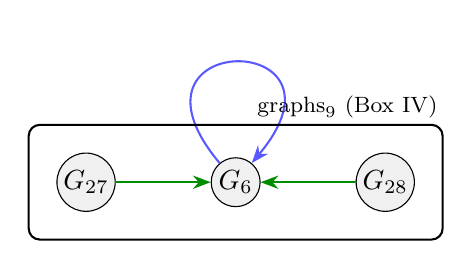
\begin{tikzpicture}[
  font=\normalsize,
  >=Stealth,
  grnode/.style={circle, draw=black, fill=gray!12, minimum size=6.2mm, inner sep=1pt},
  stepmap/.style={->, draw=blue!65, line width=0.75pt},
  permmap/.style={->, draw=green!55!black, line width=0.75pt}
]
  \node[grnode] (v6) at (0.00,0.00) {$G_{6}$};
  \node[grnode] (v27) at (-1.90,0.00) {$G_{27}$};
  \node[grnode] (v28) at (1.90,0.00) {$G_{28}$};
  \draw[stepmap] (v6) to[out=130,in=50,looseness=14] (v6);
  \draw[permmap] (v27) -- (v6);
  \draw[permmap] (v28) -- (v6);
  \node[draw=black, line width=0.75pt, rounded corners=4pt, inner sep=10pt, fit=(v6)(v27)(v28)] (boxframe) {};
  \node[anchor=south east, inner sep=2pt, font=\footnotesize] at (boxframe.north east) {$\mathrm{graphs}_{9}$ (Box $\mathrm{IV}$)};
\end{tikzpicture}
\end{center}
\begingroup\sloppy\normalsize\noindent
\raggedright
\textbf{Graph data (ltt structures in this box).}\par\smallskip\begin{enumerate}[leftmargin=*, itemsep=2pt]
\item $G_{6}$:
\begin{itemize}[leftmargin=*, itemsep=0pt]
\item underlying graph class $= U_3$.
\item red vertex $= \bar{x}_{2}$.
\item red edge $= \{\bar{x}_{1},\,\bar{x}_{2}\}$.
\item purple edges ($|\mathcal{P}|=9$):\mbox{}\\$P_{1}: \{x_{1},\,x_{3}\},\; \{x_{1},\,\bar{x}_{1}\},\; \{x_{3},\,\bar{x}_{1}\}$\\
$P_{2}: \{x_{2},\,x_{4}\},\; \{x_{2},\,x_{5}\},\; \{x_{4},\,x_{5}\}$\\
$P_{3}: \{\bar{x}_{3},\,\bar{x}_{4}\},\; \{\bar{x}_{3},\,\bar{x}_{5}\},\; \{\bar{x}_{4},\,\bar{x}_{5}\}$.
\item black edges ($|\mathcal{B}|=5$): $\{x_{1},\,\bar{x}_{1}\},\; \{x_{2},\,\bar{x}_{2}\},\; \{x_{3},\,\bar{x}_{3}\},\; \{x_{4},\,\bar{x}_{4}\},\; \{x_{5},\,\bar{x}_{5}\}$.
\end{itemize}
\item $G_{27}$:
\begin{itemize}[leftmargin=*, itemsep=0pt]
\item underlying graph class $= U_3$.
\item red vertex $= x_{3}$.
\item red edge $= \{x_{1},\,x_{3}\}$.
\item purple edges ($|\mathcal{P}|=9$):\mbox{}\\$P_{1}: \{x_{1},\,\bar{x}_{1}\},\; \{x_{1},\,\bar{x}_{2}\},\; \{\bar{x}_{1},\,\bar{x}_{2}\}$\\
$P_{2}: \{x_{2},\,x_{4}\},\; \{x_{2},\,x_{5}\},\; \{x_{4},\,x_{5}\}$\\
$P_{3}: \{\bar{x}_{3},\,\bar{x}_{4}\},\; \{\bar{x}_{3},\,\bar{x}_{5}\},\; \{\bar{x}_{4},\,\bar{x}_{5}\}$.
\item black edges ($|\mathcal{B}|=5$): $\{x_{1},\,\bar{x}_{1}\},\; \{x_{2},\,\bar{x}_{2}\},\; \{x_{3},\,\bar{x}_{3}\},\; \{x_{4},\,\bar{x}_{4}\},\; \{x_{5},\,\bar{x}_{5}\}$.
\end{itemize}
\item $G_{28}$:
\begin{itemize}[leftmargin=*, itemsep=0pt]
\item underlying graph class $= U_3$.
\item red vertex $= x_{3}$.
\item red edge $= \{x_{3},\,\bar{x}_{1}\}$.
\item purple edges ($|\mathcal{P}|=9$):\mbox{}\\$P_{1}: \{x_{1},\,\bar{x}_{1}\},\; \{x_{1},\,\bar{x}_{2}\},\; \{\bar{x}_{1},\,\bar{x}_{2}\}$\\
$P_{2}: \{x_{2},\,x_{4}\},\; \{x_{2},\,x_{5}\},\; \{x_{4},\,x_{5}\}$\\
$P_{3}: \{\bar{x}_{3},\,\bar{x}_{4}\},\; \{\bar{x}_{3},\,\bar{x}_{5}\},\; \{\bar{x}_{4},\,\bar{x}_{5}\}$.
\item black edges ($|\mathcal{B}|=5$): $\{x_{1},\,\bar{x}_{1}\},\; \{x_{2},\,\bar{x}_{2}\},\; \{x_{3},\,\bar{x}_{3}\},\; \{x_{4},\,\bar{x}_{4}\},\; \{x_{5},\,\bar{x}_{5}\}$.
\end{itemize}
\end{enumerate}
\par\medskip
\textbf{Arrows.}\; Blue: Step~$2$ edge label. Green: permutation $\varphi$ from ep-isomorphism (Step~$3$). \par\smallskip\textbf{Maps represented (internal to Box~$\mathrm{IV}$).}
\begin{enumerate}[leftmargin=*, itemsep=2pt]
\item $G_{27} \xrightarrow{\varphi} G_{6}$, where $\varphi=x_{1} \mapsto \bar{x}_{1},\; x_{2} \mapsto \bar{x}_{3},\; x_{3} \mapsto \bar{x}_{2},\; x_{4} \mapsto \bar{x}_{4},\; x_{5} \mapsto \bar{x}_{5}$ \textit{(permutation / ep-isomorphism).}
\item $G_{28} \xrightarrow{\varphi} G_{6}$, where $\varphi=x_{1} \mapsto x_{1},\; x_{2} \mapsto \bar{x}_{3},\; x_{3} \mapsto \bar{x}_{2},\; x_{4} \mapsto \bar{x}_{4},\; x_{5} \mapsto \bar{x}_{5}$ \textit{(permutation / ep-isomorphism).}
\item $G_{6} \xrightarrow{\bar{x}_{2} \to x_{1}\,\bar{x}_{2}} G_{6}$ \textit{(Step~2)}.
\end{enumerate}
\par\medskip
\textbf{Incoming preAUT edges (into this box).}\par\smallskip
\begin{enumerate}[leftmargin=*, itemsep=2pt]
\item $G_{1} \xrightarrow{\bar{x}_{2} \to x_{1}\,\bar{x}_{2}} G_{6}$ {\footnotesize ($\mathrm{graphs}_{6}$, Box $\mathrm{III}$)} \textit{(Step~2)}.
\item $G_{19} \xrightarrow{x_{3} \to \bar{x}_{1}\,x_{3}} G_{27}$ {\footnotesize ($\mathrm{graphs}_{12}$, Box $\mathrm{V}$)} \textit{(Step~2)}.
\item $G_{19} \xrightarrow{x_{3} \to x_{1}\,x_{3}} G_{28}$ {\footnotesize ($\mathrm{graphs}_{12}$, Box $\mathrm{V}$)} \textit{(Step~2)}.
\end{enumerate}
\par\medskip
\textbf{Outgoing preAUT edges (from this box).}\par\smallskip
\begin{enumerate}[leftmargin=*, itemsep=2pt]
\item $G_{6} \xrightarrow{x_{3} \to \bar{x}_{2}\,x_{3}} G_{10}$ {\footnotesize ($\mathrm{graphs}_{4}$, Box $\mathrm{VIII}$)} \textit{(Step~2)}.
\item $G_{6} \xrightarrow{\bar{x}_{2} \to x_{3}\,\bar{x}_{2}} G_{11}$ {\footnotesize ($\mathrm{graphs}_{4}$, Box $\mathrm{VIII}$)} \textit{(Step~2)}.
\item $G_{6} \xrightarrow{x_{1} \to \bar{x}_{2}\,x_{1}} G_{5}$ {\footnotesize ($\mathrm{graphs}_{1}$, Box $\mathrm{II}$)} \textit{(Step~2)}.
\end{enumerate}
\par\endgroup

\subsection*{Class $12$ (Box $\mathrm{V}$): internal preAUT maps}

\begin{center}
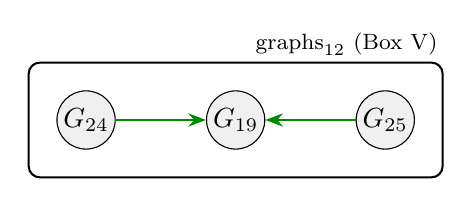
\begin{tikzpicture}[
  font=\normalsize,
  >=Stealth,
  grnode/.style={circle, draw=black, fill=gray!12, minimum size=6.2mm, inner sep=1pt},
  stepmap/.style={->, draw=blue!65, line width=0.75pt},
  permmap/.style={->, draw=green!55!black, line width=0.75pt}
]
  \node[grnode] (v19) at (0.00,0.00) {$G_{19}$};
  \node[grnode] (v24) at (-1.90,0.00) {$G_{24}$};
  \node[grnode] (v25) at (1.90,0.00) {$G_{25}$};
  \draw[permmap] (v24) -- (v19);
  \draw[permmap] (v25) -- (v19);
  \node[draw=black, line width=0.75pt, rounded corners=4pt, inner sep=10pt, fit=(v19)(v24)(v25)] (boxframe) {};
  \node[anchor=south east, inner sep=2pt, font=\footnotesize] at (boxframe.north east) {$\mathrm{graphs}_{12}$ (Box $\mathrm{V}$)};
\end{tikzpicture}
\end{center}
\begingroup\sloppy\normalsize\noindent
\raggedright
\textbf{Graph data (ltt structures in this box).}\par\smallskip\begin{enumerate}[leftmargin=*, itemsep=2pt]
\item $G_{19}$:
\begin{itemize}[leftmargin=*, itemsep=0pt]
\item underlying graph class $= U_3$.
\item red vertex $= x_{3}$.
\item red edge $= \{x_{3},\,\bar{x}_{2}\}$.
\item purple edges ($|\mathcal{P}|=9$):\mbox{}\\$P_{1}: \{x_{1},\,\bar{x}_{1}\},\; \{x_{1},\,\bar{x}_{2}\},\; \{\bar{x}_{1},\,\bar{x}_{2}\}$\\
$P_{2}: \{x_{2},\,x_{4}\},\; \{x_{2},\,x_{5}\},\; \{x_{4},\,x_{5}\}$\\
$P_{3}: \{\bar{x}_{3},\,\bar{x}_{4}\},\; \{\bar{x}_{3},\,\bar{x}_{5}\},\; \{\bar{x}_{4},\,\bar{x}_{5}\}$.
\item black edges ($|\mathcal{B}|=5$): $\{x_{1},\,\bar{x}_{1}\},\; \{x_{2},\,\bar{x}_{2}\},\; \{x_{3},\,\bar{x}_{3}\},\; \{x_{4},\,\bar{x}_{4}\},\; \{x_{5},\,\bar{x}_{5}\}$.
\end{itemize}
\item $G_{24}$:
\begin{itemize}[leftmargin=*, itemsep=0pt]
\item underlying graph class $= U_3$.
\item red vertex $= \bar{x}_{4}$.
\item red edge $= \{\bar{x}_{2},\,\bar{x}_{4}\}$.
\item purple edges ($|\mathcal{P}|=9$):\mbox{}\\$P_{1}: \{x_{1},\,\bar{x}_{1}\},\; \{x_{1},\,\bar{x}_{2}\},\; \{\bar{x}_{1},\,\bar{x}_{2}\}$\\
$P_{2}: \{x_{2},\,\bar{x}_{3}\},\; \{x_{2},\,\bar{x}_{5}\},\; \{\bar{x}_{3},\,\bar{x}_{5}\}$\\
$P_{3}: \{x_{3},\,x_{4}\},\; \{x_{3},\,x_{5}\},\; \{x_{4},\,x_{5}\}$.
\item black edges ($|\mathcal{B}|=5$): $\{x_{1},\,\bar{x}_{1}\},\; \{x_{2},\,\bar{x}_{2}\},\; \{x_{3},\,\bar{x}_{3}\},\; \{x_{4},\,\bar{x}_{4}\},\; \{x_{5},\,\bar{x}_{5}\}$.
\end{itemize}
\item $G_{25}$:
\begin{itemize}[leftmargin=*, itemsep=0pt]
\item underlying graph class $= U_3$.
\item red vertex $= \bar{x}_{5}$.
\item red edge $= \{\bar{x}_{2},\,\bar{x}_{5}\}$.
\item purple edges ($|\mathcal{P}|=9$):\mbox{}\\$P_{1}: \{x_{1},\,\bar{x}_{1}\},\; \{x_{1},\,\bar{x}_{2}\},\; \{\bar{x}_{1},\,\bar{x}_{2}\}$\\
$P_{2}: \{x_{2},\,\bar{x}_{3}\},\; \{x_{2},\,\bar{x}_{4}\},\; \{\bar{x}_{3},\,\bar{x}_{4}\}$\\
$P_{3}: \{x_{3},\,x_{4}\},\; \{x_{3},\,x_{5}\},\; \{x_{4},\,x_{5}\}$.
\item black edges ($|\mathcal{B}|=5$): $\{x_{1},\,\bar{x}_{1}\},\; \{x_{2},\,\bar{x}_{2}\},\; \{x_{3},\,\bar{x}_{3}\},\; \{x_{4},\,\bar{x}_{4}\},\; \{x_{5},\,\bar{x}_{5}\}$.
\end{itemize}
\end{enumerate}
\par\medskip
\textbf{Arrows.}\; Blue: Step~$2$ edge label. Green: permutation $\varphi$ from ep-isomorphism (Step~$3$). \par\smallskip\textbf{Maps represented (internal to Box~$\mathrm{V}$).}
\begin{enumerate}[leftmargin=*, itemsep=2pt]
\item $G_{24} \xrightarrow{\varphi} G_{19}$, where $\varphi=x_{1} \mapsto x_{1},\; x_{2} \mapsto x_{2},\; x_{3} \mapsto \bar{x}_{4},\; x_{4} \mapsto \bar{x}_{3},\; x_{5} \mapsto \bar{x}_{5}$ \textit{(permutation / ep-isomorphism).}
\item $G_{25} \xrightarrow{\varphi} G_{19}$, where $\varphi=x_{1} \mapsto x_{1},\; x_{2} \mapsto x_{2},\; x_{3} \mapsto \bar{x}_{4},\; x_{4} \mapsto \bar{x}_{5},\; x_{5} \mapsto \bar{x}_{3}$ \textit{(permutation / ep-isomorphism).}
\end{enumerate}
\par\medskip
\textbf{Incoming preAUT edges (into this box).}\par\smallskip
\begin{enumerate}[leftmargin=*, itemsep=2pt]
\item $G_{16} \xrightarrow{x_{3} \to x_{2}\,x_{3}} G_{19}$ {\footnotesize ($\mathrm{graphs}_{5}$, Box $\mathrm{VI}$)} \textit{(Step~2)}.
\item $G_{18} \xrightarrow{\bar{x}_{4} \to x_{2}\,\bar{x}_{4}} G_{24}$ {\footnotesize ($\mathrm{graphs}_{3}$, Box $\mathrm{VII}$)} \textit{(Step~2)}.
\item $G_{18} \xrightarrow{\bar{x}_{5} \to x_{2}\,\bar{x}_{5}} G_{25}$ {\footnotesize ($\mathrm{graphs}_{3}$, Box $\mathrm{VII}$)} \textit{(Step~2)}.
\end{enumerate}
\par\medskip
\textbf{Outgoing preAUT edges (from this box).}\par\smallskip
\begin{enumerate}[leftmargin=*, itemsep=2pt]
\item $G_{19} \xrightarrow{x_{1} \to x_{3}\,x_{1}} G_{26}$ {\footnotesize ($\mathrm{graphs}_{1}$, Box $\mathrm{II}$)} \textit{(Step~2)}.
\item $G_{19} \xrightarrow{x_{3} \to \bar{x}_{1}\,x_{3}} G_{27}$ {\footnotesize ($\mathrm{graphs}_{9}$, Box $\mathrm{IV}$)} \textit{(Step~2)}.
\item $G_{19} \xrightarrow{x_{3} \to x_{1}\,x_{3}} G_{28}$ {\footnotesize ($\mathrm{graphs}_{9}$, Box $\mathrm{IV}$)} \textit{(Step~2)}.
\item $G_{19} \xrightarrow{\bar{x}_{1} \to x_{3}\,\bar{x}_{1}} G_{29}$ {\footnotesize ($\mathrm{graphs}_{1}$, Box $\mathrm{II}$)} \textit{(Step~2)}.
\end{enumerate}
\par\endgroup

\subsection*{Class $5$ (Box $\mathrm{VI}$): internal preAUT maps}

\begin{center}
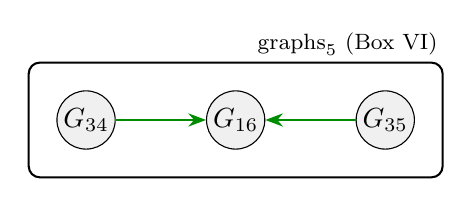
\begin{tikzpicture}[
  font=\normalsize,
  >=Stealth,
  grnode/.style={circle, draw=black, fill=gray!12, minimum size=6.2mm, inner sep=1pt},
  stepmap/.style={->, draw=blue!65, line width=0.75pt},
  permmap/.style={->, draw=green!55!black, line width=0.75pt}
]
  \node[grnode] (v16) at (0.00,0.00) {$G_{16}$};
  \node[grnode] (v34) at (-1.90,0.00) {$G_{34}$};
  \node[grnode] (v35) at (1.90,0.00) {$G_{35}$};
  \draw[permmap] (v34) -- (v16);
  \draw[permmap] (v35) -- (v16);
  \node[draw=black, line width=0.75pt, rounded corners=4pt, inner sep=10pt, fit=(v16)(v34)(v35)] (boxframe) {};
  \node[anchor=south east, inner sep=2pt, font=\footnotesize] at (boxframe.north east) {$\mathrm{graphs}_{5}$ (Box $\mathrm{VI}$)};
\end{tikzpicture}
\end{center}
\begingroup\sloppy\normalsize\noindent
\raggedright
\textbf{Graph data (ltt structures in this box).}\par\smallskip\begin{enumerate}[leftmargin=*, itemsep=2pt]
\item $G_{16}$:
\begin{itemize}[leftmargin=*, itemsep=0pt]
\item underlying graph class $= U_4$.
\item red vertex $= x_{3}$.
\item red edge $= \{x_{3},\,x_{5}\}$.
\item purple edges ($|\mathcal{P}|=9$):\mbox{}\\$P_{1}: \{x_{1},\,\bar{x}_{1}\},\; \{x_{1},\,\bar{x}_{2}\},\; \{\bar{x}_{1},\,\bar{x}_{2}\}$\\
$P_{2}: \{x_{2},\,x_{4}\},\; \{x_{2},\,x_{5}\},\; \{x_{4},\,x_{5}\}$\\
$P_{3}: \{\bar{x}_{3},\,\bar{x}_{4}\},\; \{\bar{x}_{3},\,\bar{x}_{5}\},\; \{\bar{x}_{4},\,\bar{x}_{5}\}$.
\item black edges ($|\mathcal{B}|=5$): $\{x_{1},\,\bar{x}_{1}\},\; \{x_{2},\,\bar{x}_{2}\},\; \{x_{3},\,\bar{x}_{3}\},\; \{x_{4},\,\bar{x}_{4}\},\; \{x_{5},\,\bar{x}_{5}\}$.
\end{itemize}
\item $G_{34}$:
\begin{itemize}[leftmargin=*, itemsep=0pt]
\item underlying graph class $= U_4$.
\item red vertex $= x_{1}$.
\item red edge $= \{x_{1},\,x_{4}\}$.
\item purple edges ($|\mathcal{P}|=9$):\mbox{}\\$P_{1}: \{x_{2},\,x_{4}\},\; \{x_{2},\,x_{5}\},\; \{x_{4},\,x_{5}\}$\\
$P_{2}: \{x_{3},\,\bar{x}_{3}\},\; \{x_{3},\,\bar{x}_{5}\},\; \{\bar{x}_{3},\,\bar{x}_{5}\}$\\
$P_{3}: \{\bar{x}_{1},\,\bar{x}_{2}\},\; \{\bar{x}_{1},\,\bar{x}_{4}\},\; \{\bar{x}_{2},\,\bar{x}_{4}\}$.
\item black edges ($|\mathcal{B}|=5$): $\{x_{1},\,\bar{x}_{1}\},\; \{x_{2},\,\bar{x}_{2}\},\; \{x_{3},\,\bar{x}_{3}\},\; \{x_{4},\,\bar{x}_{4}\},\; \{x_{5},\,\bar{x}_{5}\}$.
\end{itemize}
\item $G_{35}$:
\begin{itemize}[leftmargin=*, itemsep=0pt]
\item underlying graph class $= U_4$.
\item red vertex $= \bar{x}_{1}$.
\item red edge $= \{x_{4},\,\bar{x}_{1}\}$.
\item purple edges ($|\mathcal{P}|=9$):\mbox{}\\$P_{1}: \{x_{1},\,\bar{x}_{2}\},\; \{x_{1},\,\bar{x}_{4}\},\; \{\bar{x}_{2},\,\bar{x}_{4}\}$\\
$P_{2}: \{x_{2},\,x_{4}\},\; \{x_{2},\,x_{5}\},\; \{x_{4},\,x_{5}\}$\\
$P_{3}: \{x_{3},\,\bar{x}_{3}\},\; \{x_{3},\,\bar{x}_{5}\},\; \{\bar{x}_{3},\,\bar{x}_{5}\}$.
\item black edges ($|\mathcal{B}|=5$): $\{x_{1},\,\bar{x}_{1}\},\; \{x_{2},\,\bar{x}_{2}\},\; \{x_{3},\,\bar{x}_{3}\},\; \{x_{4},\,\bar{x}_{4}\},\; \{x_{5},\,\bar{x}_{5}\}$.
\end{itemize}
\end{enumerate}
\par\medskip
\textbf{Arrows.}\; Blue: Step~$2$ edge label. Green: permutation $\varphi$ from ep-isomorphism (Step~$3$). \par\smallskip\textbf{Maps represented (internal to Box~$\mathrm{VI}$).}
\begin{enumerate}[leftmargin=*, itemsep=2pt]
\item $G_{34} \xrightarrow{\varphi} G_{16}$, where $\varphi=x_{1} \mapsto x_{3},\; x_{2} \mapsto x_{4},\; x_{3} \mapsto x_{1},\; x_{4} \mapsto x_{5},\; x_{5} \mapsto x_{2}$ \textit{(permutation / ep-isomorphism).}
\item $G_{35} \xrightarrow{\varphi} G_{16}$, where $\varphi=x_{1} \mapsto \bar{x}_{3},\; x_{2} \mapsto x_{4},\; x_{3} \mapsto x_{1},\; x_{4} \mapsto x_{5},\; x_{5} \mapsto x_{2}$ \textit{(permutation / ep-isomorphism).}
\end{enumerate}
\par\medskip
\textbf{Incoming preAUT edges (into this box).}\par\smallskip
\begin{enumerate}[leftmargin=*, itemsep=2pt]
\item $G_{12} \xrightarrow{x_{3} \to \bar{x}_{5}\,x_{3}} G_{16}$ {\footnotesize ($\mathrm{graphs}_{7}$, Box $\mathrm{X}$)} \textit{(Step~2)}.
\item $G_{17} \xrightarrow{x_{3} \to \bar{x}_{5}\,x_{3}} G_{16}$ {\footnotesize ($\mathrm{graphs}_{10}$, Box $\mathrm{IX}$)} \textit{(Step~2)}.
\item $G_{31} \xrightarrow{x_{1} \to \bar{x}_{4}\,x_{1}} G_{34}$ {\footnotesize ($\mathrm{graphs}_{13}$, Box $\mathrm{XI}$)} \textit{(Step~2)}.
\item $G_{31} \xrightarrow{\bar{x}_{1} \to \bar{x}_{4}\,\bar{x}_{1}} G_{35}$ {\footnotesize ($\mathrm{graphs}_{13}$, Box $\mathrm{XI}$)} \textit{(Step~2)}.
\end{enumerate}
\par\medskip
\textbf{Outgoing preAUT edges (from this box).}\par\smallskip
\begin{enumerate}[leftmargin=*, itemsep=2pt]
\item $G_{16} \xrightarrow{x_{3} \to x_{4}\,x_{3}} G_{12}$ {\footnotesize ($\mathrm{graphs}_{7}$, Box $\mathrm{X}$)} \textit{(Step~2)}.
\item $G_{16} \xrightarrow{x_{4} \to x_{3}\,x_{4}} G_{14}$ {\footnotesize ($\mathrm{graphs}_{7}$, Box $\mathrm{X}$)} \textit{(Step~2)}.
\item $G_{16} \xrightarrow{x_{2} \to x_{3}\,x_{2}} G_{18}$ {\footnotesize ($\mathrm{graphs}_{3}$, Box $\mathrm{VII}$)} \textit{(Step~2)}.
\item $G_{16} \xrightarrow{x_{3} \to x_{2}\,x_{3}} G_{19}$ {\footnotesize ($\mathrm{graphs}_{12}$, Box $\mathrm{V}$)} \textit{(Step~2)}.
\end{enumerate}
\par\endgroup

\subsection*{Class $3$ (Box $\mathrm{VII}$): internal preAUT maps}

\begin{center}
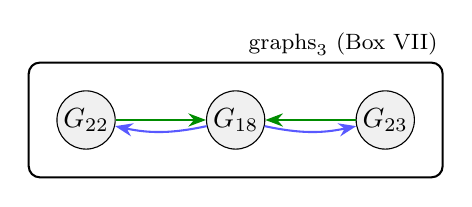
\begin{tikzpicture}[
  font=\normalsize,
  >=Stealth,
  grnode/.style={circle, draw=black, fill=gray!12, minimum size=6.2mm, inner sep=1pt},
  stepmap/.style={->, draw=blue!65, line width=0.75pt},
  permmap/.style={->, draw=green!55!black, line width=0.75pt}
]
  \node[grnode] (v18) at (0.00,0.00) {$G_{18}$};
  \node[grnode] (v22) at (-1.90,0.00) {$G_{22}$};
  \node[grnode] (v23) at (1.90,0.00) {$G_{23}$};
  \draw[stepmap] (v18) to[bend left=12] (v22);
  \draw[permmap] (v22) -- (v18);
  \draw[stepmap] (v18) to[bend right=12] (v23);
  \draw[permmap] (v23) -- (v18);
  \node[draw=black, line width=0.75pt, rounded corners=4pt, inner sep=10pt, fit=(v18)(v22)(v23)] (boxframe) {};
  \node[anchor=south east, inner sep=2pt, font=\footnotesize] at (boxframe.north east) {$\mathrm{graphs}_{3}$ (Box $\mathrm{VII}$)};
\end{tikzpicture}
\end{center}
\begingroup\sloppy\normalsize\noindent
\raggedright
\textbf{Graph data (ltt structures in this box).}\par\smallskip\begin{enumerate}[leftmargin=*, itemsep=2pt]
\item $G_{18}$:
\begin{itemize}[leftmargin=*, itemsep=0pt]
\item underlying graph class $= U_4$.
\item red vertex $= x_{2}$.
\item red edge $= \{x_{2},\,\bar{x}_{3}\}$.
\item purple edges ($|\mathcal{P}|=9$):\mbox{}\\$P_{1}: \{x_{1},\,\bar{x}_{1}\},\; \{x_{1},\,\bar{x}_{2}\},\; \{\bar{x}_{1},\,\bar{x}_{2}\}$\\
$P_{2}: \{x_{3},\,x_{4}\},\; \{x_{3},\,x_{5}\},\; \{x_{4},\,x_{5}\}$\\
$P_{3}: \{\bar{x}_{3},\,\bar{x}_{4}\},\; \{\bar{x}_{3},\,\bar{x}_{5}\},\; \{\bar{x}_{4},\,\bar{x}_{5}\}$.
\item black edges ($|\mathcal{B}|=5$): $\{x_{1},\,\bar{x}_{1}\},\; \{x_{2},\,\bar{x}_{2}\},\; \{x_{3},\,\bar{x}_{3}\},\; \{x_{4},\,\bar{x}_{4}\},\; \{x_{5},\,\bar{x}_{5}\}$.
\end{itemize}
\item $G_{22}$:
\begin{itemize}[leftmargin=*, itemsep=0pt]
\item underlying graph class $= U_4$.
\item red vertex $= x_{2}$.
\item red edge $= \{x_{2},\,x_{4}\}$.
\item purple edges ($|\mathcal{P}|=9$):\mbox{}\\$P_{1}: \{x_{1},\,\bar{x}_{1}\},\; \{x_{1},\,\bar{x}_{2}\},\; \{\bar{x}_{1},\,\bar{x}_{2}\}$\\
$P_{2}: \{x_{3},\,x_{4}\},\; \{x_{3},\,x_{5}\},\; \{x_{4},\,x_{5}\}$\\
$P_{3}: \{\bar{x}_{3},\,\bar{x}_{4}\},\; \{\bar{x}_{3},\,\bar{x}_{5}\},\; \{\bar{x}_{4},\,\bar{x}_{5}\}$.
\item black edges ($|\mathcal{B}|=5$): $\{x_{1},\,\bar{x}_{1}\},\; \{x_{2},\,\bar{x}_{2}\},\; \{x_{3},\,\bar{x}_{3}\},\; \{x_{4},\,\bar{x}_{4}\},\; \{x_{5},\,\bar{x}_{5}\}$.
\end{itemize}
\item $G_{23}$:
\begin{itemize}[leftmargin=*, itemsep=0pt]
\item underlying graph class $= U_4$.
\item red vertex $= x_{2}$.
\item red edge $= \{x_{2},\,x_{5}\}$.
\item purple edges ($|\mathcal{P}|=9$):\mbox{}\\$P_{1}: \{x_{1},\,\bar{x}_{1}\},\; \{x_{1},\,\bar{x}_{2}\},\; \{\bar{x}_{1},\,\bar{x}_{2}\}$\\
$P_{2}: \{x_{3},\,x_{4}\},\; \{x_{3},\,x_{5}\},\; \{x_{4},\,x_{5}\}$\\
$P_{3}: \{\bar{x}_{3},\,\bar{x}_{4}\},\; \{\bar{x}_{3},\,\bar{x}_{5}\},\; \{\bar{x}_{4},\,\bar{x}_{5}\}$.
\item black edges ($|\mathcal{B}|=5$): $\{x_{1},\,\bar{x}_{1}\},\; \{x_{2},\,\bar{x}_{2}\},\; \{x_{3},\,\bar{x}_{3}\},\; \{x_{4},\,\bar{x}_{4}\},\; \{x_{5},\,\bar{x}_{5}\}$.
\end{itemize}
\end{enumerate}
\par\medskip
\textbf{Arrows.}\; Blue: Step~$2$ edge label. Green: permutation $\varphi$ from ep-isomorphism (Step~$3$). \par\smallskip\textbf{Maps represented (internal to Box~$\mathrm{VII}$).}
\begin{enumerate}[leftmargin=*, itemsep=2pt]
\item $G_{18} \xrightarrow{x_{2} \to \bar{x}_{4}\,x_{2}} G_{22}$ \textit{(Step~2)}.
\item $G_{18} \xrightarrow{x_{2} \to \bar{x}_{5}\,x_{2}} G_{23}$ \textit{(Step~2)}.
\item $G_{22} \xrightarrow{\varphi} G_{18}$, where $\varphi=x_{1} \mapsto x_{1},\; x_{2} \mapsto x_{2},\; x_{3} \mapsto \bar{x}_{4},\; x_{4} \mapsto \bar{x}_{3},\; x_{5} \mapsto \bar{x}_{5}$ \textit{(permutation / ep-isomorphism).}
\item $G_{23} \xrightarrow{\varphi} G_{18}$, where $\varphi=x_{1} \mapsto x_{1},\; x_{2} \mapsto x_{2},\; x_{3} \mapsto \bar{x}_{4},\; x_{4} \mapsto \bar{x}_{5},\; x_{5} \mapsto \bar{x}_{3}$ \textit{(permutation / ep-isomorphism).}
\end{enumerate}
\par\medskip
\textbf{Incoming preAUT edges (into this box).}\par\smallskip
\begin{enumerate}[leftmargin=*, itemsep=2pt]
\item $G_{16} \xrightarrow{x_{2} \to x_{3}\,x_{2}} G_{18}$ {\footnotesize ($\mathrm{graphs}_{5}$, Box $\mathrm{VI}$)} \textit{(Step~2)}.
\end{enumerate}
\par\medskip
\textbf{Outgoing preAUT edges (from this box).}\par\smallskip
\begin{enumerate}[leftmargin=*, itemsep=2pt]
\item $G_{18} \xrightarrow{\bar{x}_{4} \to x_{2}\,\bar{x}_{4}} G_{24}$ {\footnotesize ($\mathrm{graphs}_{12}$, Box $\mathrm{V}$)} \textit{(Step~2)}.
\item $G_{18} \xrightarrow{\bar{x}_{5} \to x_{2}\,\bar{x}_{5}} G_{25}$ {\footnotesize ($\mathrm{graphs}_{12}$, Box $\mathrm{V}$)} \textit{(Step~2)}.
\end{enumerate}
\par\endgroup

\subsection*{Class $4$ (Box $\mathrm{VIII}$): internal preAUT maps}

\begin{center}
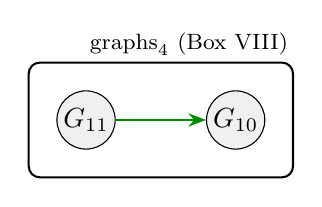
\begin{tikzpicture}[
  font=\normalsize,
  >=Stealth,
  grnode/.style={circle, draw=black, fill=gray!12, minimum size=6.2mm, inner sep=1pt},
  stepmap/.style={->, draw=blue!65, line width=0.75pt},
  permmap/.style={->, draw=green!55!black, line width=0.75pt}
]
  \node[grnode] (v10) at (0.95,0.00) {$G_{10}$};
  \node[grnode] (v11) at (-0.95,0.00) {$G_{11}$};
  \draw[permmap] (v11) -- (v10);
  \node[draw=black, line width=0.75pt, rounded corners=4pt, inner sep=10pt, fit=(v10)(v11)] (boxframe) {};
  \node[anchor=south east, inner sep=2pt, font=\footnotesize] at (boxframe.north east) {$\mathrm{graphs}_{4}$ (Box $\mathrm{VIII}$)};
\end{tikzpicture}
\end{center}
\begingroup\sloppy\normalsize\noindent
\raggedright
\textbf{Graph data (ltt structures in this box).}\par\smallskip\begin{enumerate}[leftmargin=*, itemsep=2pt]
\item $G_{10}$:
\begin{itemize}[leftmargin=*, itemsep=0pt]
\item underlying graph class $= U_4$.
\item red vertex $= x_{3}$.
\item red edge $= \{x_{2},\,x_{3}\}$.
\item purple edges ($|\mathcal{P}|=9$):\mbox{}\\$P_{1}: \{x_{1},\,\bar{x}_{1}\},\; \{x_{1},\,\bar{x}_{2}\},\; \{\bar{x}_{1},\,\bar{x}_{2}\}$\\
$P_{2}: \{x_{2},\,x_{4}\},\; \{x_{2},\,x_{5}\},\; \{x_{4},\,x_{5}\}$\\
$P_{3}: \{\bar{x}_{3},\,\bar{x}_{4}\},\; \{\bar{x}_{3},\,\bar{x}_{5}\},\; \{\bar{x}_{4},\,\bar{x}_{5}\}$.
\item black edges ($|\mathcal{B}|=5$): $\{x_{1},\,\bar{x}_{1}\},\; \{x_{2},\,\bar{x}_{2}\},\; \{x_{3},\,\bar{x}_{3}\},\; \{x_{4},\,\bar{x}_{4}\},\; \{x_{5},\,\bar{x}_{5}\}$.
\end{itemize}
\item $G_{11}$:
\begin{itemize}[leftmargin=*, itemsep=0pt]
\item underlying graph class $= U_4$.
\item red vertex $= \bar{x}_{2}$.
\item red edge $= \{\bar{x}_{2},\,\bar{x}_{3}\}$.
\item purple edges ($|\mathcal{P}|=9$):\mbox{}\\$P_{1}: \{x_{1},\,x_{3}\},\; \{x_{1},\,\bar{x}_{1}\},\; \{x_{3},\,\bar{x}_{1}\}$\\
$P_{2}: \{x_{2},\,x_{4}\},\; \{x_{2},\,x_{5}\},\; \{x_{4},\,x_{5}\}$\\
$P_{3}: \{\bar{x}_{3},\,\bar{x}_{4}\},\; \{\bar{x}_{3},\,\bar{x}_{5}\},\; \{\bar{x}_{4},\,\bar{x}_{5}\}$.
\item black edges ($|\mathcal{B}|=5$): $\{x_{1},\,\bar{x}_{1}\},\; \{x_{2},\,\bar{x}_{2}\},\; \{x_{3},\,\bar{x}_{3}\},\; \{x_{4},\,\bar{x}_{4}\},\; \{x_{5},\,\bar{x}_{5}\}$.
\end{itemize}
\end{enumerate}
\par\medskip
\textbf{Arrows.}\; Blue: Step~$2$ edge label. Green: permutation $\varphi$ from ep-isomorphism (Step~$3$). \par\smallskip\textbf{Maps represented (internal to Box~$\mathrm{VIII}$).}
\begin{enumerate}[leftmargin=*, itemsep=2pt]
\item $G_{11} \xrightarrow{\varphi} G_{10}$, where $\varphi=x_{1} \mapsto x_{1},\; x_{2} \mapsto \bar{x}_{3},\; x_{3} \mapsto \bar{x}_{2},\; x_{4} \mapsto \bar{x}_{4},\; x_{5} \mapsto \bar{x}_{5}$ \textit{(permutation / ep-isomorphism).}
\end{enumerate}
\par\medskip
\textbf{Incoming preAUT edges (into this box).}\par\smallskip
\begin{enumerate}[leftmargin=*, itemsep=2pt]
\item $G_{6} \xrightarrow{x_{3} \to \bar{x}_{2}\,x_{3}} G_{10}$ {\footnotesize ($\mathrm{graphs}_{9}$, Box $\mathrm{IV}$)} \textit{(Step~2)}.
\item $G_{6} \xrightarrow{\bar{x}_{2} \to x_{3}\,\bar{x}_{2}} G_{11}$ {\footnotesize ($\mathrm{graphs}_{9}$, Box $\mathrm{IV}$)} \textit{(Step~2)}.
\end{enumerate}
\par\medskip
\textbf{Outgoing preAUT edges (from this box).}\par\smallskip
\begin{enumerate}[leftmargin=*, itemsep=2pt]
\item $G_{10} \xrightarrow{x_{3} \to x_{4}\,x_{3}} G_{12}$ {\footnotesize ($\mathrm{graphs}_{7}$, Box $\mathrm{X}$)} \textit{(Step~2)}.
\item $G_{10} \xrightarrow{x_{3} \to x_{5}\,x_{3}} G_{13}$ {\footnotesize ($\mathrm{graphs}_{7}$, Box $\mathrm{X}$)} \textit{(Step~2)}.
\item $G_{10} \xrightarrow{x_{4} \to x_{3}\,x_{4}} G_{14}$ {\footnotesize ($\mathrm{graphs}_{7}$, Box $\mathrm{X}$)} \textit{(Step~2)}.
\item $G_{10} \xrightarrow{x_{5} \to x_{3}\,x_{5}} G_{15}$ {\footnotesize ($\mathrm{graphs}_{7}$, Box $\mathrm{X}$)} \textit{(Step~2)}.
\end{enumerate}
\par\endgroup

\subsection*{Class $10$ (Box $\mathrm{IX}$): internal preAUT maps}

\begin{center}
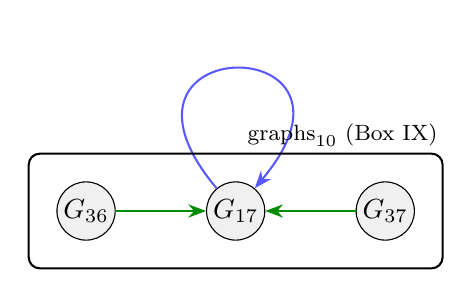
\begin{tikzpicture}[
  font=\normalsize,
  >=Stealth,
  grnode/.style={circle, draw=black, fill=gray!12, minimum size=6.2mm, inner sep=1pt},
  stepmap/.style={->, draw=blue!65, line width=0.75pt},
  permmap/.style={->, draw=green!55!black, line width=0.75pt}
]
  \node[grnode] (v17) at (0.00,0.00) {$G_{17}$};
  \node[grnode] (v36) at (-1.90,0.00) {$G_{36}$};
  \node[grnode] (v37) at (1.90,0.00) {$G_{37}$};
  \draw[stepmap] (v17) to[out=130,in=50,looseness=14] (v17);
  \draw[permmap] (v36) -- (v17);
  \draw[permmap] (v37) -- (v17);
  \node[draw=black, line width=0.75pt, rounded corners=4pt, inner sep=10pt, fit=(v17)(v36)(v37)] (boxframe) {};
  \node[anchor=south east, inner sep=2pt, font=\footnotesize] at (boxframe.north east) {$\mathrm{graphs}_{10}$ (Box $\mathrm{IX}$)};
\end{tikzpicture}
\end{center}
\begingroup\sloppy\normalsize\noindent
\raggedright
\textbf{Graph data (ltt structures in this box).}\par\smallskip\begin{enumerate}[leftmargin=*, itemsep=2pt]
\item $G_{17}$:
\begin{itemize}[leftmargin=*, itemsep=0pt]
\item underlying graph class $= U_1$.
\item red vertex $= \bar{x}_{5}$.
\item red edge $= \{\bar{x}_{3},\,\bar{x}_{5}\}$.
\item purple edges ($|\mathcal{P}|=9$):\mbox{}\\$P_{1}: \{x_{1},\,\bar{x}_{1}\},\; \{x_{1},\,\bar{x}_{2}\},\; \{\bar{x}_{1},\,\bar{x}_{2}\}$\\
$P_{2}: \{x_{2},\,x_{4}\},\; \{x_{2},\,x_{5}\},\; \{x_{4},\,x_{5}\}$\\
$P_{3}: \{x_{3},\,\bar{x}_{3}\},\; \{x_{3},\,\bar{x}_{4}\},\; \{\bar{x}_{3},\,\bar{x}_{4}\}$.
\item black edges ($|\mathcal{B}|=5$): $\{x_{1},\,\bar{x}_{1}\},\; \{x_{2},\,\bar{x}_{2}\},\; \{x_{3},\,\bar{x}_{3}\},\; \{x_{4},\,\bar{x}_{4}\},\; \{x_{5},\,\bar{x}_{5}\}$.
\end{itemize}
\item $G_{36}$:
\begin{itemize}[leftmargin=*, itemsep=0pt]
\item underlying graph class $= U_1$.
\item red vertex $= \bar{x}_{4}$.
\item red edge $= \{x_{1},\,\bar{x}_{4}\}$.
\item purple edges ($|\mathcal{P}|=9$):\mbox{}\\$P_{1}: \{x_{1},\,\bar{x}_{1}\},\; \{x_{1},\,\bar{x}_{2}\},\; \{\bar{x}_{1},\,\bar{x}_{2}\}$\\
$P_{2}: \{x_{2},\,x_{4}\},\; \{x_{2},\,x_{5}\},\; \{x_{4},\,x_{5}\}$\\
$P_{3}: \{x_{3},\,\bar{x}_{3}\},\; \{x_{3},\,\bar{x}_{5}\},\; \{\bar{x}_{3},\,\bar{x}_{5}\}$.
\item black edges ($|\mathcal{B}|=5$): $\{x_{1},\,\bar{x}_{1}\},\; \{x_{2},\,\bar{x}_{2}\},\; \{x_{3},\,\bar{x}_{3}\},\; \{x_{4},\,\bar{x}_{4}\},\; \{x_{5},\,\bar{x}_{5}\}$.
\end{itemize}
\item $G_{37}$:
\begin{itemize}[leftmargin=*, itemsep=0pt]
\item underlying graph class $= U_1$.
\item red vertex $= \bar{x}_{4}$.
\item red edge $= \{\bar{x}_{1},\,\bar{x}_{4}\}$.
\item purple edges ($|\mathcal{P}|=9$):\mbox{}\\$P_{1}: \{x_{1},\,\bar{x}_{1}\},\; \{x_{1},\,\bar{x}_{2}\},\; \{\bar{x}_{1},\,\bar{x}_{2}\}$\\
$P_{2}: \{x_{2},\,x_{4}\},\; \{x_{2},\,x_{5}\},\; \{x_{4},\,x_{5}\}$\\
$P_{3}: \{x_{3},\,\bar{x}_{3}\},\; \{x_{3},\,\bar{x}_{5}\},\; \{\bar{x}_{3},\,\bar{x}_{5}\}$.
\item black edges ($|\mathcal{B}|=5$): $\{x_{1},\,\bar{x}_{1}\},\; \{x_{2},\,\bar{x}_{2}\},\; \{x_{3},\,\bar{x}_{3}\},\; \{x_{4},\,\bar{x}_{4}\},\; \{x_{5},\,\bar{x}_{5}\}$.
\end{itemize}
\end{enumerate}
\par\medskip
\textbf{Arrows.}\; Blue: Step~$2$ edge label. Green: permutation $\varphi$ from ep-isomorphism (Step~$3$). \par\smallskip\textbf{Maps represented (internal to Box~$\mathrm{IX}$).}
\begin{enumerate}[leftmargin=*, itemsep=2pt]
\item $G_{17} \xrightarrow{\bar{x}_{5} \to x_{3}\,\bar{x}_{5}} G_{17}$ \textit{(Step~2)}.
\item $G_{36} \xrightarrow{\varphi} G_{17}$, where $\varphi=x_{1} \mapsto \bar{x}_{3},\; x_{2} \mapsto x_{4},\; x_{3} \mapsto x_{1},\; x_{4} \mapsto x_{5},\; x_{5} \mapsto x_{2}$ \textit{(permutation / ep-isomorphism).}
\item $G_{37} \xrightarrow{\varphi} G_{17}$, where $\varphi=x_{1} \mapsto x_{3},\; x_{2} \mapsto x_{4},\; x_{3} \mapsto x_{1},\; x_{4} \mapsto x_{5},\; x_{5} \mapsto x_{2}$ \textit{(permutation / ep-isomorphism).}
\end{enumerate}
\par\medskip
\textbf{Incoming preAUT edges (into this box).}\par\smallskip
\begin{enumerate}[leftmargin=*, itemsep=2pt]
\item $G_{12} \xrightarrow{\bar{x}_{5} \to x_{3}\,\bar{x}_{5}} G_{17}$ {\footnotesize ($\mathrm{graphs}_{7}$, Box $\mathrm{X}$)} \textit{(Step~2)}.
\item $G_{31} \xrightarrow{\bar{x}_{4} \to \bar{x}_{1}\,\bar{x}_{4}} G_{36}$ {\footnotesize ($\mathrm{graphs}_{13}$, Box $\mathrm{XI}$)} \textit{(Step~2)}.
\item $G_{31} \xrightarrow{\bar{x}_{4} \to x_{1}\,\bar{x}_{4}} G_{37}$ {\footnotesize ($\mathrm{graphs}_{13}$, Box $\mathrm{XI}$)} \textit{(Step~2)}.
\end{enumerate}
\par\medskip
\textbf{Outgoing preAUT edges (from this box).}\par\smallskip
\begin{enumerate}[leftmargin=*, itemsep=2pt]
\item $G_{17} \xrightarrow{x_{3} \to \bar{x}_{5}\,x_{3}} G_{16}$ {\footnotesize ($\mathrm{graphs}_{5}$, Box $\mathrm{VI}$)} \textit{(Step~2)}.
\item $G_{17} \xrightarrow{\bar{x}_{4} \to \bar{x}_{5}\,\bar{x}_{4}} G_{20}$ {\footnotesize ($\mathrm{graphs}_{8}$, Box $\mathrm{XII}$)} \textit{(Step~2)}.
\item $G_{17} \xrightarrow{\bar{x}_{5} \to \bar{x}_{4}\,\bar{x}_{5}} G_{21}$ {\footnotesize ($\mathrm{graphs}_{8}$, Box $\mathrm{XII}$)} \textit{(Step~2)}.
\end{enumerate}
\par\endgroup

\subsection*{Class $7$ (Box $\mathrm{X}$): internal preAUT maps}

\begin{center}
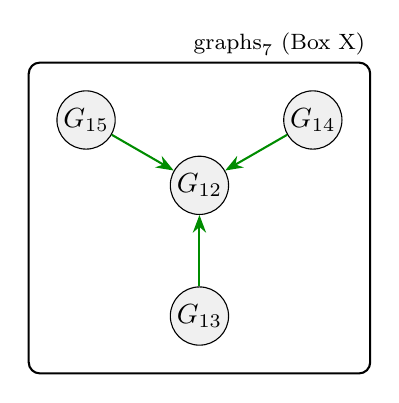
\begin{tikzpicture}[
  font=\normalsize,
  >=Stealth,
  grnode/.style={circle, draw=black, fill=gray!12, minimum size=6.2mm, inner sep=1pt},
  stepmap/.style={->, draw=blue!65, line width=0.75pt},
  permmap/.style={->, draw=green!55!black, line width=0.75pt}
]
  \node[grnode] (v12) at (0.00,0.00) {$G_{12}$};
  \node[grnode] (v13) at (0.00,-1.66) {$G_{13}$};
  \node[grnode] (v14) at (1.44,0.83) {$G_{14}$};
  \node[grnode] (v15) at (-1.44,0.83) {$G_{15}$};
  \draw[permmap] (v13) -- (v12);
  \draw[permmap] (v14) -- (v12);
  \draw[permmap] (v15) -- (v12);
  \node[draw=black, line width=0.75pt, rounded corners=4pt, inner sep=10pt, fit=(v12)(v13)(v14)(v15)] (boxframe) {};
  \node[anchor=south east, inner sep=2pt, font=\footnotesize] at (boxframe.north east) {$\mathrm{graphs}_{7}$ (Box $\mathrm{X}$)};
\end{tikzpicture}
\end{center}
\begingroup\sloppy\normalsize\noindent
\raggedright
\textbf{Graph data (ltt structures in this box).}\par\smallskip\begin{enumerate}[leftmargin=*, itemsep=2pt]
\item $G_{12}$:
\begin{itemize}[leftmargin=*, itemsep=0pt]
\item underlying graph class $= U_1$.
\item red vertex $= x_{3}$.
\item red edge $= \{x_{3},\,\bar{x}_{4}\}$.
\item purple edges ($|\mathcal{P}|=9$):\mbox{}\\$P_{1}: \{x_{1},\,\bar{x}_{1}\},\; \{x_{1},\,\bar{x}_{2}\},\; \{\bar{x}_{1},\,\bar{x}_{2}\}$\\
$P_{2}: \{x_{2},\,x_{4}\},\; \{x_{2},\,x_{5}\},\; \{x_{4},\,x_{5}\}$\\
$P_{3}: \{\bar{x}_{3},\,\bar{x}_{4}\},\; \{\bar{x}_{3},\,\bar{x}_{5}\},\; \{\bar{x}_{4},\,\bar{x}_{5}\}$.
\item black edges ($|\mathcal{B}|=5$): $\{x_{1},\,\bar{x}_{1}\},\; \{x_{2},\,\bar{x}_{2}\},\; \{x_{3},\,\bar{x}_{3}\},\; \{x_{4},\,\bar{x}_{4}\},\; \{x_{5},\,\bar{x}_{5}\}$.
\end{itemize}
\item $G_{13}$:
\begin{itemize}[leftmargin=*, itemsep=0pt]
\item underlying graph class $= U_1$.
\item red vertex $= x_{3}$.
\item red edge $= \{x_{3},\,\bar{x}_{5}\}$.
\item purple edges ($|\mathcal{P}|=9$):\mbox{}\\$P_{1}: \{x_{1},\,\bar{x}_{1}\},\; \{x_{1},\,\bar{x}_{2}\},\; \{\bar{x}_{1},\,\bar{x}_{2}\}$\\
$P_{2}: \{x_{2},\,x_{4}\},\; \{x_{2},\,x_{5}\},\; \{x_{4},\,x_{5}\}$\\
$P_{3}: \{\bar{x}_{3},\,\bar{x}_{4}\},\; \{\bar{x}_{3},\,\bar{x}_{5}\},\; \{\bar{x}_{4},\,\bar{x}_{5}\}$.
\item black edges ($|\mathcal{B}|=5$): $\{x_{1},\,\bar{x}_{1}\},\; \{x_{2},\,\bar{x}_{2}\},\; \{x_{3},\,\bar{x}_{3}\},\; \{x_{4},\,\bar{x}_{4}\},\; \{x_{5},\,\bar{x}_{5}\}$.
\end{itemize}
\item $G_{14}$:
\begin{itemize}[leftmargin=*, itemsep=0pt]
\item underlying graph class $= U_1$.
\item red vertex $= x_{4}$.
\item red edge $= \{x_{4},\,\bar{x}_{3}\}$.
\item purple edges ($|\mathcal{P}|=9$):\mbox{}\\$P_{1}: \{x_{1},\,\bar{x}_{1}\},\; \{x_{1},\,\bar{x}_{2}\},\; \{\bar{x}_{1},\,\bar{x}_{2}\}$\\
$P_{2}: \{x_{2},\,x_{3}\},\; \{x_{2},\,x_{5}\},\; \{x_{3},\,x_{5}\}$\\
$P_{3}: \{\bar{x}_{3},\,\bar{x}_{4}\},\; \{\bar{x}_{3},\,\bar{x}_{5}\},\; \{\bar{x}_{4},\,\bar{x}_{5}\}$.
\item black edges ($|\mathcal{B}|=5$): $\{x_{1},\,\bar{x}_{1}\},\; \{x_{2},\,\bar{x}_{2}\},\; \{x_{3},\,\bar{x}_{3}\},\; \{x_{4},\,\bar{x}_{4}\},\; \{x_{5},\,\bar{x}_{5}\}$.
\end{itemize}
\item $G_{15}$:
\begin{itemize}[leftmargin=*, itemsep=0pt]
\item underlying graph class $= U_1$.
\item red vertex $= x_{5}$.
\item red edge $= \{x_{5},\,\bar{x}_{3}\}$.
\item purple edges ($|\mathcal{P}|=9$):\mbox{}\\$P_{1}: \{x_{1},\,\bar{x}_{1}\},\; \{x_{1},\,\bar{x}_{2}\},\; \{\bar{x}_{1},\,\bar{x}_{2}\}$\\
$P_{2}: \{x_{2},\,x_{3}\},\; \{x_{2},\,x_{4}\},\; \{x_{3},\,x_{4}\}$\\
$P_{3}: \{\bar{x}_{3},\,\bar{x}_{4}\},\; \{\bar{x}_{3},\,\bar{x}_{5}\},\; \{\bar{x}_{4},\,\bar{x}_{5}\}$.
\item black edges ($|\mathcal{B}|=5$): $\{x_{1},\,\bar{x}_{1}\},\; \{x_{2},\,\bar{x}_{2}\},\; \{x_{3},\,\bar{x}_{3}\},\; \{x_{4},\,\bar{x}_{4}\},\; \{x_{5},\,\bar{x}_{5}\}$.
\end{itemize}
\end{enumerate}
\par\medskip
\textbf{Arrows.}\; Blue: Step~$2$ edge label. Green: permutation $\varphi$ from ep-isomorphism (Step~$3$). \par\smallskip\textbf{Maps represented (internal to Box~$\mathrm{X}$).}
\begin{enumerate}[leftmargin=*, itemsep=2pt]
\item $G_{13} \xrightarrow{\varphi} G_{12}$, where $\varphi=x_{1} \mapsto x_{1},\; x_{2} \mapsto x_{2},\; x_{3} \mapsto x_{3},\; x_{4} \mapsto x_{5},\; x_{5} \mapsto x_{4}$ \textit{(permutation / ep-isomorphism).}
\item $G_{14} \xrightarrow{\varphi} G_{12}$, where $\varphi=x_{1} \mapsto x_{1},\; x_{2} \mapsto x_{2},\; x_{3} \mapsto x_{4},\; x_{4} \mapsto x_{3},\; x_{5} \mapsto x_{5}$ \textit{(permutation / ep-isomorphism).}
\item $G_{15} \xrightarrow{\varphi} G_{12}$, where $\varphi=x_{1} \mapsto x_{1},\; x_{2} \mapsto x_{2},\; x_{3} \mapsto x_{4},\; x_{4} \mapsto x_{5},\; x_{5} \mapsto x_{3}$ \textit{(permutation / ep-isomorphism).}
\end{enumerate}
\par\medskip
\textbf{Incoming preAUT edges (into this box).}\par\smallskip
\begin{enumerate}[leftmargin=*, itemsep=2pt]
\item $G_{10} \xrightarrow{x_{3} \to x_{4}\,x_{3}} G_{12}$ {\footnotesize ($\mathrm{graphs}_{4}$, Box $\mathrm{VIII}$)} \textit{(Step~2)}.
\item $G_{10} \xrightarrow{x_{3} \to x_{5}\,x_{3}} G_{13}$ {\footnotesize ($\mathrm{graphs}_{4}$, Box $\mathrm{VIII}$)} \textit{(Step~2)}.
\item $G_{10} \xrightarrow{x_{4} \to x_{3}\,x_{4}} G_{14}$ {\footnotesize ($\mathrm{graphs}_{4}$, Box $\mathrm{VIII}$)} \textit{(Step~2)}.
\item $G_{10} \xrightarrow{x_{5} \to x_{3}\,x_{5}} G_{15}$ {\footnotesize ($\mathrm{graphs}_{4}$, Box $\mathrm{VIII}$)} \textit{(Step~2)}.
\item $G_{16} \xrightarrow{x_{3} \to x_{4}\,x_{3}} G_{12}$ {\footnotesize ($\mathrm{graphs}_{5}$, Box $\mathrm{VI}$)} \textit{(Step~2)}.
\item $G_{16} \xrightarrow{x_{4} \to x_{3}\,x_{4}} G_{14}$ {\footnotesize ($\mathrm{graphs}_{5}$, Box $\mathrm{VI}$)} \textit{(Step~2)}.
\end{enumerate}
\par\medskip
\textbf{Outgoing preAUT edges (from this box).}\par\smallskip
\begin{enumerate}[leftmargin=*, itemsep=2pt]
\item $G_{12} \xrightarrow{x_{3} \to \bar{x}_{5}\,x_{3}} G_{16}$ {\footnotesize ($\mathrm{graphs}_{5}$, Box $\mathrm{VI}$)} \textit{(Step~2)}.
\item $G_{12} \xrightarrow{\bar{x}_{5} \to x_{3}\,\bar{x}_{5}} G_{17}$ {\footnotesize ($\mathrm{graphs}_{10}$, Box $\mathrm{IX}$)} \textit{(Step~2)}.
\end{enumerate}
\par\endgroup

\subsection*{Class $13$ (Box $\mathrm{XI}$): internal preAUT maps}

\begin{center}
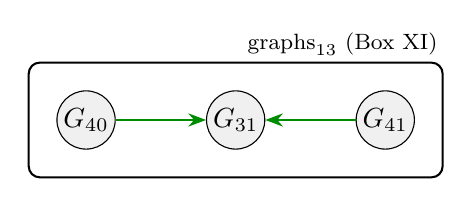
\begin{tikzpicture}[
  font=\normalsize,
  >=Stealth,
  grnode/.style={circle, draw=black, fill=gray!12, minimum size=6.2mm, inner sep=1pt},
  stepmap/.style={->, draw=blue!65, line width=0.75pt},
  permmap/.style={->, draw=green!55!black, line width=0.75pt}
]
  \node[grnode] (v31) at (0.00,0.00) {$G_{31}$};
  \node[grnode] (v40) at (-1.90,0.00) {$G_{40}$};
  \node[grnode] (v41) at (1.90,0.00) {$G_{41}$};
  \draw[permmap] (v40) -- (v31);
  \draw[permmap] (v41) -- (v31);
  \node[draw=black, line width=0.75pt, rounded corners=4pt, inner sep=10pt, fit=(v31)(v40)(v41)] (boxframe) {};
  \node[anchor=south east, inner sep=2pt, font=\footnotesize] at (boxframe.north east) {$\mathrm{graphs}_{13}$ (Box $\mathrm{XI}$)};
\end{tikzpicture}
\end{center}
\begingroup\sloppy\normalsize\noindent
\raggedright
\textbf{Graph data (ltt structures in this box).}\par\smallskip\begin{enumerate}[leftmargin=*, itemsep=2pt]
\item $G_{31}$:
\begin{itemize}[leftmargin=*, itemsep=0pt]
\item underlying graph class $= U_1$.
\item red vertex $= \bar{x}_{4}$.
\item red edge $= \{\bar{x}_{2},\,\bar{x}_{4}\}$.
\item purple edges ($|\mathcal{P}|=9$):\mbox{}\\$P_{1}: \{x_{1},\,\bar{x}_{1}\},\; \{x_{1},\,\bar{x}_{2}\},\; \{\bar{x}_{1},\,\bar{x}_{2}\}$\\
$P_{2}: \{x_{2},\,x_{4}\},\; \{x_{2},\,x_{5}\},\; \{x_{4},\,x_{5}\}$\\
$P_{3}: \{x_{3},\,\bar{x}_{3}\},\; \{x_{3},\,\bar{x}_{5}\},\; \{\bar{x}_{3},\,\bar{x}_{5}\}$.
\item black edges ($|\mathcal{B}|=5$): $\{x_{1},\,\bar{x}_{1}\},\; \{x_{2},\,\bar{x}_{2}\},\; \{x_{3},\,\bar{x}_{3}\},\; \{x_{4},\,\bar{x}_{4}\},\; \{x_{5},\,\bar{x}_{5}\}$.
\end{itemize}
\item $G_{40}$:
\begin{itemize}[leftmargin=*, itemsep=0pt]
\item underlying graph class $= U_1$.
\item red vertex $= x_{3}$.
\item red edge $= \{x_{3},\,\bar{x}_{2}\}$.
\item purple edges ($|\mathcal{P}|=9$):\mbox{}\\$P_{1}: \{x_{1},\,\bar{x}_{1}\},\; \{x_{1},\,\bar{x}_{2}\},\; \{\bar{x}_{1},\,\bar{x}_{2}\}$\\
$P_{2}: \{x_{2},\,\bar{x}_{3}\},\; \{x_{2},\,\bar{x}_{5}\},\; \{\bar{x}_{3},\,\bar{x}_{5}\}$\\
$P_{3}: \{x_{4},\,x_{5}\},\; \{x_{4},\,\bar{x}_{4}\},\; \{x_{5},\,\bar{x}_{4}\}$.
\item black edges ($|\mathcal{B}|=5$): $\{x_{1},\,\bar{x}_{1}\},\; \{x_{2},\,\bar{x}_{2}\},\; \{x_{3},\,\bar{x}_{3}\},\; \{x_{4},\,\bar{x}_{4}\},\; \{x_{5},\,\bar{x}_{5}\}$.
\end{itemize}
\item $G_{41}$:
\begin{itemize}[leftmargin=*, itemsep=0pt]
\item underlying graph class $= U_1$.
\item red vertex $= \bar{x}_{3}$.
\item red edge $= \{\bar{x}_{2},\,\bar{x}_{3}\}$.
\item purple edges ($|\mathcal{P}|=9$):\mbox{}\\$P_{1}: \{x_{1},\,\bar{x}_{1}\},\; \{x_{1},\,\bar{x}_{2}\},\; \{\bar{x}_{1},\,\bar{x}_{2}\}$\\
$P_{2}: \{x_{2},\,x_{3}\},\; \{x_{2},\,\bar{x}_{5}\},\; \{x_{3},\,\bar{x}_{5}\}$\\
$P_{3}: \{x_{4},\,x_{5}\},\; \{x_{4},\,\bar{x}_{4}\},\; \{x_{5},\,\bar{x}_{4}\}$.
\item black edges ($|\mathcal{B}|=5$): $\{x_{1},\,\bar{x}_{1}\},\; \{x_{2},\,\bar{x}_{2}\},\; \{x_{3},\,\bar{x}_{3}\},\; \{x_{4},\,\bar{x}_{4}\},\; \{x_{5},\,\bar{x}_{5}\}$.
\end{itemize}
\end{enumerate}
\par\medskip
\textbf{Arrows.}\; Blue: Step~$2$ edge label. Green: permutation $\varphi$ from ep-isomorphism (Step~$3$). \par\smallskip\textbf{Maps represented (internal to Box~$\mathrm{XI}$).}
\begin{enumerate}[leftmargin=*, itemsep=2pt]
\item $G_{40} \xrightarrow{\varphi} G_{31}$, where $\varphi=x_{1} \mapsto x_{1},\; x_{2} \mapsto x_{2},\; x_{3} \mapsto \bar{x}_{4},\; x_{4} \mapsto x_{3},\; x_{5} \mapsto \bar{x}_{5}$ \textit{(permutation / ep-isomorphism).}
\item $G_{41} \xrightarrow{\varphi} G_{31}$, where $\varphi=x_{1} \mapsto x_{1},\; x_{2} \mapsto x_{2},\; x_{3} \mapsto x_{4},\; x_{4} \mapsto x_{3},\; x_{5} \mapsto \bar{x}_{5}$ \textit{(permutation / ep-isomorphism).}
\end{enumerate}
\par\medskip
\textbf{Incoming preAUT edges (into this box).}\par\smallskip
\begin{enumerate}[leftmargin=*, itemsep=2pt]
\item $G_{20} \xrightarrow{\bar{x}_{4} \to x_{2}\,\bar{x}_{4}} G_{31}$ {\footnotesize ($\mathrm{graphs}_{8}$, Box $\mathrm{XII}$)} \textit{(Step~2)}.
\item $G_{30} \xrightarrow{\bar{x}_{4} \to x_{2}\,\bar{x}_{4}} G_{31}$ {\footnotesize ($\mathrm{graphs}_{11}$, Box $\mathrm{XIII}$)} \textit{(Step~2)}.
\item $G_{32} \xrightarrow{x_{3} \to x_{2}\,x_{3}} G_{40}$ {\footnotesize ($\mathrm{graphs}_{14}$, Box $\mathrm{XIV}$)} \textit{(Step~2)}.
\item $G_{32} \xrightarrow{\bar{x}_{3} \to x_{2}\,\bar{x}_{3}} G_{41}$ {\footnotesize ($\mathrm{graphs}_{14}$, Box $\mathrm{XIV}$)} \textit{(Step~2)}.
\end{enumerate}
\par\medskip
\textbf{Outgoing preAUT edges (from this box).}\par\smallskip
\begin{enumerate}[leftmargin=*, itemsep=2pt]
\item $G_{31} \xrightarrow{x_{1} \to \bar{x}_{4}\,x_{1}} G_{34}$ {\footnotesize ($\mathrm{graphs}_{5}$, Box $\mathrm{VI}$)} \textit{(Step~2)}.
\item $G_{31} \xrightarrow{\bar{x}_{1} \to \bar{x}_{4}\,\bar{x}_{1}} G_{35}$ {\footnotesize ($\mathrm{graphs}_{5}$, Box $\mathrm{VI}$)} \textit{(Step~2)}.
\item $G_{31} \xrightarrow{\bar{x}_{4} \to \bar{x}_{1}\,\bar{x}_{4}} G_{36}$ {\footnotesize ($\mathrm{graphs}_{10}$, Box $\mathrm{IX}$)} \textit{(Step~2)}.
\item $G_{31} \xrightarrow{\bar{x}_{4} \to x_{1}\,\bar{x}_{4}} G_{37}$ {\footnotesize ($\mathrm{graphs}_{10}$, Box $\mathrm{IX}$)} \textit{(Step~2)}.
\end{enumerate}
\par\endgroup

\subsection*{Class $8$ (Box $\mathrm{XII}$): internal preAUT maps}

\begin{center}
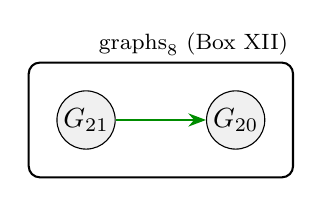
\begin{tikzpicture}[
  font=\normalsize,
  >=Stealth,
  grnode/.style={circle, draw=black, fill=gray!12, minimum size=6.2mm, inner sep=1pt},
  stepmap/.style={->, draw=blue!65, line width=0.75pt},
  permmap/.style={->, draw=green!55!black, line width=0.75pt}
]
  \node[grnode] (v20) at (0.95,0.00) {$G_{20}$};
  \node[grnode] (v21) at (-0.95,0.00) {$G_{21}$};
  \draw[permmap] (v21) -- (v20);
  \node[draw=black, line width=0.75pt, rounded corners=4pt, inner sep=10pt, fit=(v20)(v21)] (boxframe) {};
  \node[anchor=south east, inner sep=2pt, font=\footnotesize] at (boxframe.north east) {$\mathrm{graphs}_{8}$ (Box $\mathrm{XII}$)};
\end{tikzpicture}
\end{center}
\begingroup\sloppy\normalsize\noindent
\raggedright
\textbf{Graph data (ltt structures in this box).}\par\smallskip\begin{enumerate}[leftmargin=*, itemsep=2pt]
\item $G_{20}$:
\begin{itemize}[leftmargin=*, itemsep=0pt]
\item underlying graph class $= U_2$.
\item red vertex $= \bar{x}_{4}$.
\item red edge $= \{x_{5},\,\bar{x}_{4}\}$.
\item purple edges ($|\mathcal{P}|=9$):\mbox{}\\$P_{1}: \{x_{1},\,\bar{x}_{1}\},\; \{x_{1},\,\bar{x}_{2}\},\; \{\bar{x}_{1},\,\bar{x}_{2}\}$\\
$P_{2}: \{x_{2},\,x_{4}\},\; \{x_{2},\,x_{5}\},\; \{x_{4},\,x_{5}\}$\\
$P_{3}: \{x_{3},\,\bar{x}_{3}\},\; \{x_{3},\,\bar{x}_{5}\},\; \{\bar{x}_{3},\,\bar{x}_{5}\}$.
\item black edges ($|\mathcal{B}|=5$): $\{x_{1},\,\bar{x}_{1}\},\; \{x_{2},\,\bar{x}_{2}\},\; \{x_{3},\,\bar{x}_{3}\},\; \{x_{4},\,\bar{x}_{4}\},\; \{x_{5},\,\bar{x}_{5}\}$.
\end{itemize}
\item $G_{21}$:
\begin{itemize}[leftmargin=*, itemsep=0pt]
\item underlying graph class $= U_2$.
\item red vertex $= \bar{x}_{5}$.
\item red edge $= \{x_{4},\,\bar{x}_{5}\}$.
\item purple edges ($|\mathcal{P}|=9$):\mbox{}\\$P_{1}: \{x_{1},\,\bar{x}_{1}\},\; \{x_{1},\,\bar{x}_{2}\},\; \{\bar{x}_{1},\,\bar{x}_{2}\}$\\
$P_{2}: \{x_{2},\,x_{4}\},\; \{x_{2},\,x_{5}\},\; \{x_{4},\,x_{5}\}$\\
$P_{3}: \{x_{3},\,\bar{x}_{3}\},\; \{x_{3},\,\bar{x}_{4}\},\; \{\bar{x}_{3},\,\bar{x}_{4}\}$.
\item black edges ($|\mathcal{B}|=5$): $\{x_{1},\,\bar{x}_{1}\},\; \{x_{2},\,\bar{x}_{2}\},\; \{x_{3},\,\bar{x}_{3}\},\; \{x_{4},\,\bar{x}_{4}\},\; \{x_{5},\,\bar{x}_{5}\}$.
\end{itemize}
\end{enumerate}
\par\medskip
\textbf{Arrows.}\; Blue: Step~$2$ edge label. Green: permutation $\varphi$ from ep-isomorphism (Step~$3$). \par\smallskip\textbf{Maps represented (internal to Box~$\mathrm{XII}$).}
\begin{enumerate}[leftmargin=*, itemsep=2pt]
\item $G_{21} \xrightarrow{\varphi} G_{20}$, where $\varphi=x_{1} \mapsto x_{1},\; x_{2} \mapsto x_{2},\; x_{3} \mapsto x_{3},\; x_{4} \mapsto x_{5},\; x_{5} \mapsto x_{4}$ \textit{(permutation / ep-isomorphism).}
\end{enumerate}
\par\medskip
\textbf{Incoming preAUT edges (into this box).}\par\smallskip
\begin{enumerate}[leftmargin=*, itemsep=2pt]
\item $G_{17} \xrightarrow{\bar{x}_{4} \to \bar{x}_{5}\,\bar{x}_{4}} G_{20}$ {\footnotesize ($\mathrm{graphs}_{10}$, Box $\mathrm{IX}$)} \textit{(Step~2)}.
\item $G_{17} \xrightarrow{\bar{x}_{5} \to \bar{x}_{4}\,\bar{x}_{5}} G_{21}$ {\footnotesize ($\mathrm{graphs}_{10}$, Box $\mathrm{IX}$)} \textit{(Step~2)}.
\end{enumerate}
\par\medskip
\textbf{Outgoing preAUT edges (from this box).}\par\smallskip
\begin{enumerate}[leftmargin=*, itemsep=2pt]
\item $G_{20} \xrightarrow{x_{2} \to \bar{x}_{4}\,x_{2}} G_{30}$ {\footnotesize ($\mathrm{graphs}_{11}$, Box $\mathrm{XIII}$)} \textit{(Step~2)}.
\item $G_{20} \xrightarrow{\bar{x}_{4} \to x_{2}\,\bar{x}_{4}} G_{31}$ {\footnotesize ($\mathrm{graphs}_{13}$, Box $\mathrm{XI}$)} \textit{(Step~2)}.
\end{enumerate}
\par\endgroup

\subsection*{Class $11$ (Box $\mathrm{XIII}$): internal preAUT maps}

\begin{center}
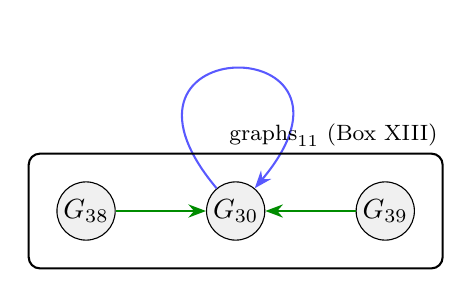
\begin{tikzpicture}[
  font=\normalsize,
  >=Stealth,
  grnode/.style={circle, draw=black, fill=gray!12, minimum size=6.2mm, inner sep=1pt},
  stepmap/.style={->, draw=blue!65, line width=0.75pt},
  permmap/.style={->, draw=green!55!black, line width=0.75pt}
]
  \node[grnode] (v30) at (0.00,0.00) {$G_{30}$};
  \node[grnode] (v38) at (-1.90,0.00) {$G_{38}$};
  \node[grnode] (v39) at (1.90,0.00) {$G_{39}$};
  \draw[stepmap] (v30) to[out=130,in=50,looseness=14] (v30);
  \draw[permmap] (v38) -- (v30);
  \draw[permmap] (v39) -- (v30);
  \node[draw=black, line width=0.75pt, rounded corners=4pt, inner sep=10pt, fit=(v30)(v38)(v39)] (boxframe) {};
  \node[anchor=south east, inner sep=2pt, font=\footnotesize] at (boxframe.north east) {$\mathrm{graphs}_{11}$ (Box $\mathrm{XIII}$)};
\end{tikzpicture}
\end{center}
\begingroup\sloppy\normalsize\noindent
\raggedright
\textbf{Graph data (ltt structures in this box).}\par\smallskip\begin{enumerate}[leftmargin=*, itemsep=2pt]
\item $G_{30}$:
\begin{itemize}[leftmargin=*, itemsep=0pt]
\item underlying graph class $= U_2$.
\item red vertex $= x_{2}$.
\item red edge $= \{x_{2},\,x_{4}\}$.
\item purple edges ($|\mathcal{P}|=9$):\mbox{}\\$P_{1}: \{x_{1},\,\bar{x}_{1}\},\; \{x_{1},\,\bar{x}_{2}\},\; \{\bar{x}_{1},\,\bar{x}_{2}\}$\\
$P_{2}: \{x_{3},\,\bar{x}_{3}\},\; \{x_{3},\,\bar{x}_{5}\},\; \{\bar{x}_{3},\,\bar{x}_{5}\}$\\
$P_{3}: \{x_{4},\,x_{5}\},\; \{x_{4},\,\bar{x}_{4}\},\; \{x_{5},\,\bar{x}_{4}\}$.
\item black edges ($|\mathcal{B}|=5$): $\{x_{1},\,\bar{x}_{1}\},\; \{x_{2},\,\bar{x}_{2}\},\; \{x_{3},\,\bar{x}_{3}\},\; \{x_{4},\,\bar{x}_{4}\},\; \{x_{5},\,\bar{x}_{5}\}$.
\end{itemize}
\item $G_{38}$:
\begin{itemize}[leftmargin=*, itemsep=0pt]
\item underlying graph class $= U_2$.
\item red vertex $= x_{2}$.
\item red edge $= \{x_{2},\,x_{3}\}$.
\item purple edges ($|\mathcal{P}|=9$):\mbox{}\\$P_{1}: \{x_{1},\,\bar{x}_{1}\},\; \{x_{1},\,\bar{x}_{2}\},\; \{\bar{x}_{1},\,\bar{x}_{2}\}$\\
$P_{2}: \{x_{3},\,\bar{x}_{3}\},\; \{x_{3},\,\bar{x}_{5}\},\; \{\bar{x}_{3},\,\bar{x}_{5}\}$\\
$P_{3}: \{x_{4},\,x_{5}\},\; \{x_{4},\,\bar{x}_{4}\},\; \{x_{5},\,\bar{x}_{4}\}$.
\item black edges ($|\mathcal{B}|=5$): $\{x_{1},\,\bar{x}_{1}\},\; \{x_{2},\,\bar{x}_{2}\},\; \{x_{3},\,\bar{x}_{3}\},\; \{x_{4},\,\bar{x}_{4}\},\; \{x_{5},\,\bar{x}_{5}\}$.
\end{itemize}
\item $G_{39}$:
\begin{itemize}[leftmargin=*, itemsep=0pt]
\item underlying graph class $= U_2$.
\item red vertex $= x_{2}$.
\item red edge $= \{x_{2},\,\bar{x}_{3}\}$.
\item purple edges ($|\mathcal{P}|=9$):\mbox{}\\$P_{1}: \{x_{1},\,\bar{x}_{1}\},\; \{x_{1},\,\bar{x}_{2}\},\; \{\bar{x}_{1},\,\bar{x}_{2}\}$\\
$P_{2}: \{x_{3},\,\bar{x}_{3}\},\; \{x_{3},\,\bar{x}_{5}\},\; \{\bar{x}_{3},\,\bar{x}_{5}\}$\\
$P_{3}: \{x_{4},\,x_{5}\},\; \{x_{4},\,\bar{x}_{4}\},\; \{x_{5},\,\bar{x}_{4}\}$.
\item black edges ($|\mathcal{B}|=5$): $\{x_{1},\,\bar{x}_{1}\},\; \{x_{2},\,\bar{x}_{2}\},\; \{x_{3},\,\bar{x}_{3}\},\; \{x_{4},\,\bar{x}_{4}\},\; \{x_{5},\,\bar{x}_{5}\}$.
\end{itemize}
\end{enumerate}
\par\medskip
\textbf{Arrows.}\; Blue: Step~$2$ edge label. Green: permutation $\varphi$ from ep-isomorphism (Step~$3$). \par\smallskip\textbf{Maps represented (internal to Box~$\mathrm{XIII}$).}
\begin{enumerate}[leftmargin=*, itemsep=2pt]
\item $G_{30} \xrightarrow{x_{2} \to \bar{x}_{4}\,x_{2}} G_{30}$ \textit{(Step~2)}.
\item $G_{38} \xrightarrow{\varphi} G_{30}$, where $\varphi=x_{1} \mapsto x_{1},\; x_{2} \mapsto x_{2},\; x_{3} \mapsto x_{4},\; x_{4} \mapsto x_{3},\; x_{5} \mapsto \bar{x}_{5}$ \textit{(permutation / ep-isomorphism).}
\item $G_{39} \xrightarrow{\varphi} G_{30}$, where $\varphi=x_{1} \mapsto x_{1},\; x_{2} \mapsto x_{2},\; x_{3} \mapsto \bar{x}_{4},\; x_{4} \mapsto x_{3},\; x_{5} \mapsto \bar{x}_{5}$ \textit{(permutation / ep-isomorphism).}
\end{enumerate}
\par\medskip
\textbf{Incoming preAUT edges (into this box).}\par\smallskip
\begin{enumerate}[leftmargin=*, itemsep=2pt]
\item $G_{20} \xrightarrow{x_{2} \to \bar{x}_{4}\,x_{2}} G_{30}$ {\footnotesize ($\mathrm{graphs}_{8}$, Box $\mathrm{XII}$)} \textit{(Step~2)}.
\item $G_{32} \xrightarrow{x_{2} \to \bar{x}_{3}\,x_{2}} G_{38}$ {\footnotesize ($\mathrm{graphs}_{14}$, Box $\mathrm{XIV}$)} \textit{(Step~2)}.
\item $G_{32} \xrightarrow{x_{2} \to x_{3}\,x_{2}} G_{39}$ {\footnotesize ($\mathrm{graphs}_{14}$, Box $\mathrm{XIV}$)} \textit{(Step~2)}.
\end{enumerate}
\par\medskip
\textbf{Outgoing preAUT edges (from this box).}\par\smallskip
\begin{enumerate}[leftmargin=*, itemsep=2pt]
\item $G_{30} \xrightarrow{\bar{x}_{4} \to x_{2}\,\bar{x}_{4}} G_{31}$ {\footnotesize ($\mathrm{graphs}_{13}$, Box $\mathrm{XI}$)} \textit{(Step~2)}.
\item $G_{30} \xrightarrow{x_{2} \to x_{5}\,x_{2}} G_{32}$ {\footnotesize ($\mathrm{graphs}_{14}$, Box $\mathrm{XIV}$)} \textit{(Step~2)}.
\item $G_{30} \xrightarrow{x_{5} \to x_{2}\,x_{5}} G_{33}$ {\footnotesize ($\mathrm{graphs}_{14}$, Box $\mathrm{XIV}$)} \textit{(Step~2)}.
\end{enumerate}
\par\endgroup

\subsection*{Class $14$ (Box $\mathrm{XIV}$): internal preAUT maps}

\begin{center}
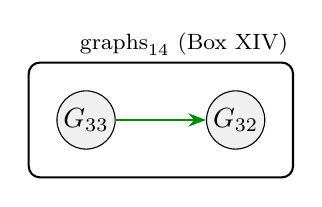
\begin{tikzpicture}[
  font=\normalsize,
  >=Stealth,
  grnode/.style={circle, draw=black, fill=gray!12, minimum size=6.2mm, inner sep=1pt},
  stepmap/.style={->, draw=blue!65, line width=0.75pt},
  permmap/.style={->, draw=green!55!black, line width=0.75pt}
]
  \node[grnode] (v32) at (0.95,0.00) {$G_{32}$};
  \node[grnode] (v33) at (-0.95,0.00) {$G_{33}$};
  \draw[permmap] (v33) -- (v32);
  \node[draw=black, line width=0.75pt, rounded corners=4pt, inner sep=10pt, fit=(v32)(v33)] (boxframe) {};
  \node[anchor=south east, inner sep=2pt, font=\footnotesize] at (boxframe.north east) {$\mathrm{graphs}_{14}$ (Box $\mathrm{XIV}$)};
\end{tikzpicture}
\end{center}
\begingroup\sloppy\normalsize\noindent
\raggedright
\textbf{Graph data (ltt structures in this box).}\par\smallskip\begin{enumerate}[leftmargin=*, itemsep=2pt]
\item $G_{32}$:
\begin{itemize}[leftmargin=*, itemsep=0pt]
\item underlying graph class $= U_2$.
\item red vertex $= x_{2}$.
\item red edge $= \{x_{2},\,\bar{x}_{5}\}$.
\item purple edges ($|\mathcal{P}|=9$):\mbox{}\\$P_{1}: \{x_{1},\,\bar{x}_{1}\},\; \{x_{1},\,\bar{x}_{2}\},\; \{\bar{x}_{1},\,\bar{x}_{2}\}$\\
$P_{2}: \{x_{3},\,\bar{x}_{3}\},\; \{x_{3},\,\bar{x}_{5}\},\; \{\bar{x}_{3},\,\bar{x}_{5}\}$\\
$P_{3}: \{x_{4},\,x_{5}\},\; \{x_{4},\,\bar{x}_{4}\},\; \{x_{5},\,\bar{x}_{4}\}$.
\item black edges ($|\mathcal{B}|=5$): $\{x_{1},\,\bar{x}_{1}\},\; \{x_{2},\,\bar{x}_{2}\},\; \{x_{3},\,\bar{x}_{3}\},\; \{x_{4},\,\bar{x}_{4}\},\; \{x_{5},\,\bar{x}_{5}\}$.
\end{itemize}
\item $G_{33}$:
\begin{itemize}[leftmargin=*, itemsep=0pt]
\item underlying graph class $= U_2$.
\item red vertex $= x_{5}$.
\item red edge $= \{x_{5},\,\bar{x}_{2}\}$.
\item purple edges ($|\mathcal{P}|=9$):\mbox{}\\$P_{1}: \{x_{1},\,\bar{x}_{1}\},\; \{x_{1},\,\bar{x}_{2}\},\; \{\bar{x}_{1},\,\bar{x}_{2}\}$\\
$P_{2}: \{x_{2},\,x_{4}\},\; \{x_{2},\,\bar{x}_{4}\},\; \{x_{4},\,\bar{x}_{4}\}$\\
$P_{3}: \{x_{3},\,\bar{x}_{3}\},\; \{x_{3},\,\bar{x}_{5}\},\; \{\bar{x}_{3},\,\bar{x}_{5}\}$.
\item black edges ($|\mathcal{B}|=5$): $\{x_{1},\,\bar{x}_{1}\},\; \{x_{2},\,\bar{x}_{2}\},\; \{x_{3},\,\bar{x}_{3}\},\; \{x_{4},\,\bar{x}_{4}\},\; \{x_{5},\,\bar{x}_{5}\}$.
\end{itemize}
\end{enumerate}
\par\medskip
\textbf{Arrows.}\; Blue: Step~$2$ edge label. Green: permutation $\varphi$ from ep-isomorphism (Step~$3$). \par\smallskip\textbf{Maps represented (internal to Box~$\mathrm{XIV}$).}
\begin{enumerate}[leftmargin=*, itemsep=2pt]
\item $G_{33} \xrightarrow{\varphi} G_{32}$, where $\varphi=x_{1} \mapsto x_{3},\; x_{2} \mapsto x_{5},\; x_{3} \mapsto x_{1},\; x_{4} \mapsto x_{4},\; x_{5} \mapsto x_{2}$ \textit{(permutation / ep-isomorphism).}
\end{enumerate}
\par\medskip
\textbf{Incoming preAUT edges (into this box).}\par\smallskip
\begin{enumerate}[leftmargin=*, itemsep=2pt]
\item $G_{30} \xrightarrow{x_{2} \to x_{5}\,x_{2}} G_{32}$ {\footnotesize ($\mathrm{graphs}_{11}$, Box $\mathrm{XIII}$)} \textit{(Step~2)}.
\item $G_{30} \xrightarrow{x_{5} \to x_{2}\,x_{5}} G_{33}$ {\footnotesize ($\mathrm{graphs}_{11}$, Box $\mathrm{XIII}$)} \textit{(Step~2)}.
\end{enumerate}
\par\medskip
\textbf{Outgoing preAUT edges (from this box).}\par\smallskip
\begin{enumerate}[leftmargin=*, itemsep=2pt]
\item $G_{32} \xrightarrow{x_{2} \to \bar{x}_{3}\,x_{2}} G_{38}$ {\footnotesize ($\mathrm{graphs}_{11}$, Box $\mathrm{XIII}$)} \textit{(Step~2)}.
\item $G_{32} \xrightarrow{x_{2} \to x_{3}\,x_{2}} G_{39}$ {\footnotesize ($\mathrm{graphs}_{11}$, Box $\mathrm{XIII}$)} \textit{(Step~2)}.
\item $G_{32} \xrightarrow{x_{3} \to x_{2}\,x_{3}} G_{40}$ {\footnotesize ($\mathrm{graphs}_{13}$, Box $\mathrm{XI}$)} \textit{(Step~2)}.
\item $G_{32} \xrightarrow{\bar{x}_{3} \to x_{2}\,\bar{x}_{3}} G_{41}$ {\footnotesize ($\mathrm{graphs}_{13}$, Box $\mathrm{XI}$)} \textit{(Step~2)}.
\end{enumerate}
\par\endgroup



\section{Working translation table: paper Roman boxes vs. code numbering}

\noindent This table gives a practical lookup between the Roman-numeral boxes in the paper image and the internal numbering used by this project (\texttt{Class \#} in the ltt-class appendix and \(\mathrm{graphs}_k\) in preAUT/AUT generation).

\begin{center}
\begin{tabular}{c|c|c}
\textbf{Paper box} & \textbf{Class \#} & \textbf{\(\mathrm{graphs}_k\)} \\
\hline
I & 2 & \(\mathrm{graphs}_2\) \\
II & 1 & \(\mathrm{graphs}_1\) \\
III & 6 & \(\mathrm{graphs}_6\) \\
IV & 9 & \(\mathrm{graphs}_9\) \\
V & 12 & \(\mathrm{graphs}_{12}\) \\
VI & 5 & \(\mathrm{graphs}_5\) \\
VII & 3 & \(\mathrm{graphs}_3\) \\
VIII & 4 & \(\mathrm{graphs}_4\) \\
IX & 10 & \(\mathrm{graphs}_{10}\) \\
X & 7 & \(\mathrm{graphs}_7\) \\
XI & 13 & \(\mathrm{graphs}_{13}\) \\
XII & 8 & \(\mathrm{graphs}_8\) \\
XIII & 11 & \(\mathrm{graphs}_{11}\) \\
XIV & 14 & \(\mathrm{graphs}_{14}\) \\
\end{tabular}
\end{center}

\end{document}
